\documentclass{book}

\title{Appunti di Misure elettroniche}
\author{Stefano Rossini}

\usepackage{bookmark}

\usepackage[italian]{babel}
\usepackage{geometry}
\geometry{a4paper, margin={2.54cm,1.9cm}}

\usepackage{hyperref}
\usepackage{tcolorbox} %for COLORED BOXES 

\usepackage{amsmath}
\usepackage{graphicx}
\graphicspath{{./immagini/}}

\usepackage{url}

\usepackage{physics}

\usepackage{amsfonts} 

\usepackage{gensymb}

\usepackage{textcomp}

\usepackage{tikz}

\usepackage{pgfplots}

\usepackage{imakeidx} 
\makeindex[columns=3, title=Alphabetical Index, intoc]

\hypersetup{
    colorlinks=true,
    linkcolor=blue,
    bookmarksnumbered=true,  % <-- numerazione nelle sezioni del PDF
    pdftitle={Appunti Misure elettroniche},
    pdfauthor={Autore},
    pdfstartview=FitH
}

\begin{document}

\maketitle

%\setcounter{chapter}{-1}
\section*{Introduzione}

 

Appunti ordinati, con approfondimenti passo-passo, del corso di Misure elettroniche per il corso di laurea in Ingegneria Elettronica 
presso l’Università Politecnica delle Marche. \newline
        



Le fonti degli appunti sono le seguenti: 

\begin{itemize}
    
    \item Slide del corso della prof.ssa Susanna Spinsante 
    "Strumentazione Digitale e Misure Elettroniche (SDME)" 
    A.A. 2024/2025 
    

\end{itemize}

La mitica Spinstante è una goat: prof stupenda, riesce a mantenere coinvolgente la materia rimanendo professionale e puntuale nella terminalogia. \newline 

Andate a lezione, se potete, perchè sono super-interessanti. \newline 

È consigliato studiare e superare prima l’esame di analisi matematica 2 e teoria dei segnali per gli indicatori statistici che saranno impiegati nel corso. \newline 

I concetti importanti dei corsi precedenti sono importanti ma non fondamentali: ci serviranno i concetti base. \newline 

Lascerò dei link a video e/o spiegazioni esterne per ulteriori approfondimenti. \newline 

Per qualsiasi domanda, scrivimi a \href{mailto:rossini.stefano.appunti@gmail.com}{rossini.stefano.appunti@gmail.com} \newline

Buono studio e buona lettura \newline

\newpage 







\tableofcontents

\section*{Tabella lettere greche utili per il corso}

\begin{center}
\begin{tabular}{ c c c }
    
Lettera maiuscola & Lettera minuscola & Nome lettera greca \\
\hline 
A & $\alpha$ & Alfa \\ \\
B & $\beta$ & Beta \\ \\
$\Gamma$ & $\gamma$ & Gamma \\ \\
$\Delta$ & $\delta$ & Delta \\ \\  
E & $\varepsilon$ & Epsilon \\ \\
H & $\eta$ & Eta  \\ \\ 
$\Theta$ & $\theta$ & Theta \\ \\  
K & $\kappa$ & Kappa \\ \\ 
$\Lambda$ & $\lambda$ & Lambda \\ \\ 
M & $\mu$ & Mu \\ \\ 
$\Pi$ & $\pi$ & Pi \\ \\ 
P & $\rho$ & Rho \\ \\
$\Sigma$ & $\sigma$ & Sigma \\ \\  
T & $\tau$ & Tau \\ \\ 
$\Phi$ & $\phi$ & Phi \\ \\
X & $\chi$ & Chi \\ \\ 
$\Psi$ & $\psi$ & Psi \\ \\ 
$\Omega$ & $\omega$ & Omega  




\end{tabular}
\end{center}

\newpage 

\chapter{Elementi di metrologia e fondamenti della misurazione}

\begin{figure}[h]
    \centering
    \includegraphics[scale = 0.45]{Misurare è conoscere.PNG}
\end{figure}  
    
\newpage 

\section{Misura e misurazione} 
\footnote{Slide della prof | SDME 1.2 Metrologia - Introduzione | pag 2-4 }

Essendo il corso chiamato "Strumentazione Digitale e Misure Elettroniche", 
è fondamentale capire cosa significa misura. \newline 

Per misura, o meglio definirla come procedimento di misura, è quel procedimento 
che porta ad assegnare un valore ad una grandezza fisica detta misurando. \newline 

Alcune osservazioni riguardo al procedimento di misura: 

\begin{itemize}
    \item Il valore assegnato al misurando è parte essenziale ma non unico del risultato di misura 
    \item La maggior parte dei procedimento di misura viene effettuata per confronto 
    \item Esistono grandezze estensive e intensive
\end{itemize}


Il risultato della misurazione è l'informazione espressa da un valore numerico, una incertezza di misura 
e dalla corrispondente unità di misura. \newline 

Si può graficare il procedimento di misura come: 

\begin{figure}[h]
    \centering
    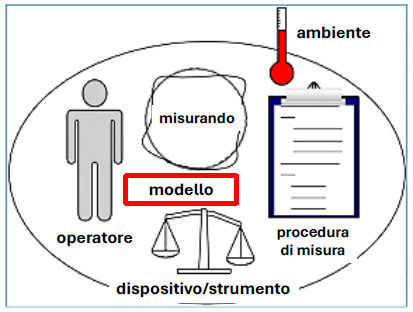
\includegraphics[scale = 0.6]{Procedimento di misura.PNG}
\end{figure}

Il metodo di misura per confronto con un riferimento o campione (unità) di misura indica 
che la quantità misurata Q si può esprimere: 

{
    \Large 
    \begin{equation}
        Q = VAL \cdot [U]
    \end{equation}
    
}

cioè un prodotto tra un valore numerico VAL e il campione o l'unità di misura [U]. \newline 

L'unità di misura è convenzionalmente una grandezza di valore unitario. \newline 

\newpage 

\section{La misurazione ideale e reale}
\footnote{Slide della prof | SDME 1.2 Metrologia - Introduzione | pag 5}


Secondo la norma UNI 4546, la misura è una informazione costituita da un valore, una incertezza ed una unità di misura, 
assegnata per rappresentare un parametro in un determinato stato del sistema. \newline 

La misurazione è un processo che mette in corrispondenza due insiemi: 
quello "reale" degli eventi fisici e quello "astratto" dei numeri. \newline 

Lo scopo della misurazione è fornire una descrizione rigorosa, quindi non soggettiva. \newline 

Utilizzando i grafici, la relazione tra il processo reale di misurazione e il mondo astratto è il seguente: 

\begin{figure}[h]
    \centering
    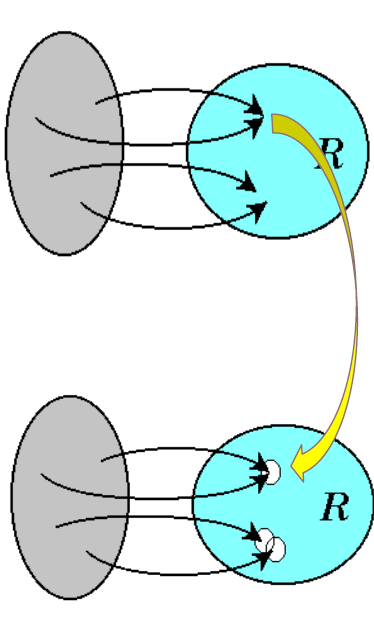
\includegraphics[scale = 0.5]{Misurazione ideale e reale.PNG}
\end{figure}

Come possiamo osservare, il processo reale di misurazione mette in corrispondenza ogni elemento 
dell'insieme degli eventi fisici con un sottoinsieme dell'insieme dei numeri. \newline 

Ciascun intervallo così determinato risulta centrato sul numero che rappresenta il "valore" del misurando. \newline 

La ampiezza dell'intervallo viene chiamata "incertezza" della misura. \newline 

\newpage 

\section{Definizione di grandezza}
\footnote{Slide della prof | SDME 1.2 Metrologia - Introduzione | pag 9}

Per grandezza si intende una quantità, proprietà, condizione usata per descrivere fenomeni e valutabile in termini di unità di misura. \newline 

Grandezza e misurando non sono la stessa cosa. \newline 

Per misurando si intende l'oggetto di una misurazione. \newline 

Le grandezze misurabili sono classificabili in 5 tipi: 

\begin{itemize}
    \item Numerale: numerazione di oggetti o singoli eventi singoli 
    \item Razionale: valori espressi da numeri razionali, cioè il rapporto tra grandezza misurata e u.d.m (unità di misura) 
    \item Strumentale: valori espressi come corrispondenza biunivoca con punti di scale convenzionali interpolabili 
    \item Complesso: valori espressi da un insieme ordinato di numeri relativi (con sistema di riferimento) 
    \item Selettivo: concerne il riconoscimento di appartenenza ad una certa classe (es: scala Mercalli)
\end{itemize}


\newpage 

\section{Conoscenza del mondo fisico e misure} 
\footnote{Slide della prof | SDME 1.2 Metrologia - Introduzione | pag 10 - 15 \\  
Appunti | 2025-02-26 | pag 2 - 6}

Grazie al VIM (Vocabolario Internazionale di Metrologia), CEI UNI 70099 (2010-04), per misurazione si intende il processo 
volto a ottenere sperimentalmente uno o più valori che possono essere ragionevolmente attribuiti a una grandezza. \newline 

Quindi la misura è una operazione di grandezza quantitativa. \newline 

Se una grandezza non si può misurare, si dice che si sta svolgendo una classificazione. \newline 

Dalle note del VIM, la misurazione non si applica a proprietà classificatorie. \newline 

Per proprietà classificatorie si intende una proprietà qualitativa di un fenomeno, corpo o sostanza, ma alla quale non è possibile associare un'espressione quantitativa. \newline 

Una misurazione si realizza mediante confronto tra grandezze o conteggio di entità. \newline 

La misurazione richiede una descrizione della grandezza o conteggio di entità. \newline 

La misurazione richiede una descrizione della grandezza adeguata all'utilizzo previsto del risultato di misura, 
una procedura di misura, un sistema di misura tarato e operante in conformità alla procedura di misura 
specificata, incluse le condizioni di misure. \newline 

Per risultato di misura si intende un insieme di valori attribuiti a un misurando congiuntamente a ogni altra informazione pertinente disponibili. \newline 

Per procedura di misura si intende una descrizione dettagliata di una misurazione eseguita in conformità a uno o più principi 
di misura e a un determinato metodo di misura, fondata su un modello di misura e comprendente tutti i calcoli necessari per ottenere un risultato di misura. \newline 

Quindi, oltre alla misura, è necessario scrivere dei procedimenti di misura, che generalmente sono dei documenti tecnici standard da compilare. \newline 

Più che strumento si parla di un sistema di misura, perché ogni oggetto influisce sul sistema (si pensa ad un cavo di bassa qualità in una misura come può danneggiare la misura stessa). \newline 

Per sistema di misura si intende un insieme di uno o più strumenti di misura e in molti casi altri dispositivi, 
ivi compresi eventuali reagenti e alimentazioni, appositamente connessi e adattati per fornire informazione 
usata, con lo scopo di stabilire, in intervalli specificanti, valori misurati di grandezze di specie specificate. \newline 

La fisica e la relazione con il mondo reale permettono di descrivere i modelli del mondo reale. \newline 

Utilizzando uno schema, possiamo visualizzarlo in questa maniera: 

\begin{figure}[h]
    \centering
    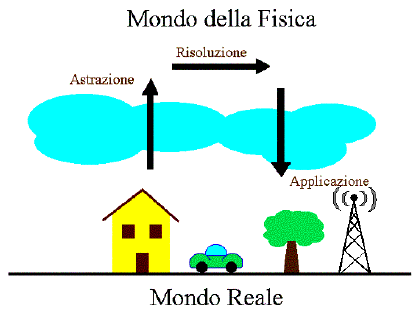
\includegraphics[scale = 0.5]{Relazione tra mondo fisico e mondo reale.PNG}
\end{figure} 


Dalla risoluzione all'applicazione, bisogna aggiungere le non idealità del mondo reale, che a sua volta, possono modificare anche l'astrazione matematica del mondo reale. \newline 

Le misure spesso si svolgono attraverso il confronto di grandezze omogenee (ad esempio nei tester si confronta la tensione da misurare con il riferimento di tensione all'interno di esso). \newline 

I riferimenti di misura sono costituiti dalle realizzazione delle definizioni di u.d.m. delle varie grandezze. \newline 

Prima di Maxwell, si prediligeva il riferimento usato dagli artefatti (ad esempio la il riferimento del chilogrammo di plato e lidio che si trova nel museo delle misure in Francia), 
mentre adesso si predilisce un riferimento assoluto, cioè basato su definizioni assolute, basate su fenomeni fisici o costanti di 
natura, che non dipendono dal tempo e dallo spazio, ritenuti "universali". \newline 

Se esiste la riferibilità, allora si può parlare di strumento di misura, sennò si parla di strumento di acquisizione. \newline 

Le relazioni tra grandezze e quindi tra u.d.m. sono esatte, poiché appartengono al mondo delle definizioni. \newline 

Le relazioni tra riferimenti di misura (realizzazioni pratiche delle u.d.m.), invece, 
non sono esatte perché i riferimenti sono affetti da imprecisioni e instabilità temporali. \newline 

L'imprecisione, vista come distanza tra realizzazione e definizione dell'u.d.m. (accuratezza) varia nel tempo. \newline 

Si impiega il termine errore nella teoria degli errori. \newline 

\newpage 

\section{Discussione qualitativa sull'incertezza di misura}
\footnote{Slide della prof | SDME 1.2 Metrologia - Introduzione | pag 16 - 25 \\  
Appunti | 2025-02-26 | pag 6 - 18}

Una grandezza fisica può essere determinata, e quindi conosciuta, soltanto ad un livello finito di incertezza. \newline 

Quanto più è bassa l'incertezza di misura, tanto più grande è il livello di conoscenza raggiunto. \newline 

Non esistono misure esatte perché l'incertezza di misura non potrà mai ridursi a zero. \newline 

Quindi si parla di incertezza di misura perché la misura comporta un intervallo di valori. \newline 

Si parla di errore solo durante la taratura di uno strumento di misura. \newline 

Quindi l'errore è diverso dall'accuratezza. \newline 

Possiamo esprimere le principali cause di incertezza: 

\begin{itemize}
    \item L'imprecisione intrinseca dei riferimenti rispetto ai quali si eseguono le misure 
    \item La conoscenza della relazione che esiste tra misurando e sistemi di misura è in genere incompleta 
    \item Le fluttuazioni naturali (rumore) limitano la risoluzione dei sistemi di rivelazione, cioè la capacità di distinguere stati vicini del misurando 
    \item La taratura per confronto o campioni di migliore qualità 
    \item Le misure avvengono in condizioni di non perfetta definizione, stabilità e controllo dei parametri ambientali, tra cui anche l'interazione dell'operatore 
    \item Gli strumenti possono presentare degli errori (ad esempio: errore di zero, errore di isteresi) 
\end{itemize}

Per essere uno strumento di misura, lo strumento deve essere riferibile rispetto alla grandezza primaria. \newline 

Quindi ci deve essere riferibilità e compatibilità. \newline 

Ci possono essere dei limiti tra strumento di misura e misurando. \newline 

Se ci sono dei valori empirici (e che quindi non si dimostrano), il valore di misura si porta dietro un'incertezza. \newline 

Il rumore comporta dei problemi nella misura perché il misurando varia nel tempo (si parla di processo stocastico). \newline 

Le fluttuazioni sono dei fenomeni generalmente distribuiti con una distribuzione gaussiana. \newline 

Inoltre, il rumore è ineliminabile. \newline 

Siccome il rumore è un processo stocastico, allora è necessario ripetere più volte la misura stessa. \newline 

In un qualunque sistema di misura, anche le u.d.m. fondamentali hanno una specifica realizzazione concreta (detta in francese mise en pratique) 
che presenta una incertezza quantificabile come lo scarto (accuratezza) rispetto alla definizione dell'u.d.m. stessa (riferimento ideale). \newline 

Tale scarto non si mantiene inalterato nel tempo (stabilità). \newline 

\newpage 

Le misure possono essere di due tipi: 

\begin{itemize}
    \item misure dirette, cioè il confronto di grandezze della stessa specie  
    \item misure indirette, cioè da un insieme di misure diverse si elabora il valore di una nuova grandezza
\end{itemize}

Non sempre è possibile una misura diretta e spesso si ricorre a una misura indiretta impiegando la relazione tra modello fisico e le varie grandezze: 
si pensi, ad esempio, alla misura della resistenza impiegando un voltmetro e un amperometro. \newline 

Avendoci a che fare con strumentazione digitale, uno dei problemi da affrontare è l'errore di quantizzazione. \newline 

Lo strumento digitale, in molti casi, è preferibile perché è più immune alle fluttuazioni dei rumori. \newline 

L'errore di quantizzazione è dovuto a strumentazione elettronica, acquisizione ed elaborazione dei segnali di tipo digitale, strumenti che includono l'ADC, e contatori elettronici. \newline 

In diversi casi è utile cambiare la risoluzione in base alla grandezza che si vuole misurare (c'è una differenza tra misurare $ \mu A$ in un circuito elettronico rispetto ai $M A$ di un impianto industriale). \newline 

La scelta della risoluzione ottimale alla misura è importante per capire se un segnale è informativo oppure se è rumore. \newline 

Utilizzando gli schemi a blocchi, possiamo rappresentare una misura come: 

\begin{figure}[h]
    \centering
    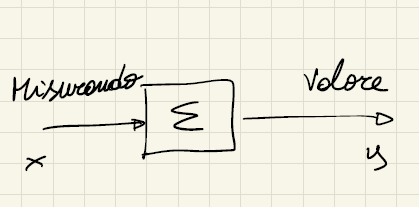
\includegraphics[scale = 0.5]{Schema a blocchi misura.PNG}
\end{figure} 

La relazione tra misurando e il valore della misura è di tipo lineare (almeno quelli che andiamo a considerare in questo corso), e quindi avremo una retta con una pendenza costante. \newline 

Possiamo scrivere: 

{
    \Large 
    \begin{equation}
        y = mx
    \end{equation}
    
}

La pendenza della retta misura la sensibilità dello strumento:

\begin{figure}[h]
    \centering
    \includegraphics[scale = 0.7]{Diverse sensibilità di uno strumento.PNG}
\end{figure} 

La maggiore sensibilità permette di misurare grandezze più piccole, più vicine al valore vero, 
allora l'uscita è facilmente leggibile. \newline 

Generalmente, un'elevata sensibilità deve essere accompagnata ad una elevata risoluzione. \newline 

In genere, in uno strumento di misura si richiede che l'uscita sia zero per segnali di ingresso nullo: 
l'errore di zero si ha quando questa condizione non è soddisfatta. \newline 

Inoltre, in uno strumento, può presentarsi un errore di isteresi, che è principalmente dovuto a sistemi di trasduzione che "immagazzinano" la carica precedente, dovuto ai componenti con memoria (come ad esempio un condensatore) presenti nello strumento stesso. \newline 

Dal punto di vista grafico, avremo un errore di isteresi in questo caso: 

\begin{figure}[h]
    \centering
    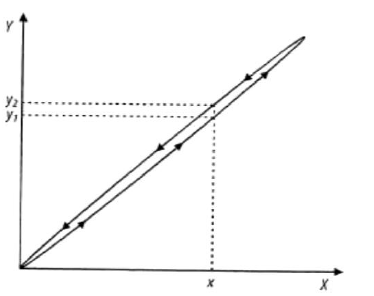
\includegraphics[scale = 0.5]{Errore di isteresi esempio.PNG}
\end{figure} 

\newpage 

\section{Un po' di terminologia} 
\footnote{Slide della prof | SDME 1.2 Metrologia - Introduzione | pag 26 - 29 \\  
Appunti | 2025-02-28 | pag 2}

Nella metrologia, il riferimento per la terminologia è il Dizionario di Metrologia, o Vocabolario Internazionale di Metrologia (VIM). \newline 

Per grandezza o quantità (misurabile) si intende un attribuito di un fenomeno o di una sostanza distinguibile qualitativamente e determinabile quantitativamente. \newline 

Dato un sistema di grandezze, si può costituire un sistema di grandezze se tra esse esistono relazione definite. \newline 

Per grandezze fondamentali (o di base) di un sistema si intende un insieme di grandezze convenzionalmente accettate come indipendenti. \newline 

Le grandezze derivate sono quelle grandezze che sono esprimibili attraverso le grandezze fondamentali. \newline 

Particolari grandezze possono adottate per convenzione come unità di misura. \newline 

Per misurando si intende una grandezza che si intende misurare. \newline 

Il risultato di una misura consiste nell'assegnare al misurando i seguenti valori: 

\begin{itemize}
    \item valore numerico 
    \item unità di misura 
    \item incertezza 
\end{itemize}

Per parametro si intende ogni caratteristica di un "sistema" alla quale è necessario assegnare valori 
per descrivere il sistema stesso, la sua evoluzione e/o le sue interazioni con altri sistemi e con l'ambiente. \newline 

Per segnale si intende la modificazione (o variazione) dello stato di un sistema usata per ottenere, elaborare e/o trasmettere un'informazione. \newline 

Per rumore, o disturbo, si intende la variazione della grandezza costituente il supporto di un segnale non correlata all'informazione da esso trasmessa. \newline 

Per incertezza si intende la stima quantitativa eseguita secondo procedimenti convenzionali, del nostro livello di non conoscenza del misurando. \newline 

Per accuratezza si intende il grado di concordanza tra un valore misurato e il valore "vero" di un misurando. \newline 

Generalmente, l'accuratezza viene data dal costruttore e/o dal laboratorio di taratura. \newline 

Si può definire l'accuratezza in base a cosa ci si riferisce: 

\begin{itemize}
    \item In riferimento ai campioni primari: è la stima dello scarto tra grandezza realizzata e definizione (esatta) dell'unità 
    \item In riferimento ad una misura: accordo che ci si attende tra il valore di misura e la migliore stima possibile per il misurando 
    \item In riferimento ad uno strumento specifico: valutazione delle differenze tra due misura di una stessa grandezza: la stima di un'incertezza dello strumento ottenuta mediante un'analisi precisa di tutte le cause di incertezza
\end{itemize}

Per ripetibilità o precisione si intende l'attitudine dello strumento o della misura a fornire, 
per uno stesso misurando, valori di lettura vicini tra loro, in letture consecutive eseguite in un breve intervallo di tempo, 
con lo stesso procedimento di misura, dallo stesso osservatore, nelle stesse condizioni per le grandezze di influenza e nello stesso luogo. \newline 

Per riproducibilità si intende la vicinanza di risultati ottenuti sullo stesso misurando in diverse specifici condizioni di misura, quindi possono cambiare principi e metodi di misura, osservatore, strumenti e riferimenti, luogo, tempo e condizioni.\newline

Per riferibilità si indica la proprietà di una misura di essere messa in relazione con quella fornita da un campione riconosciuto: si ottiene con una documentata catena ininterrotta di tarature. \newline 

Quindi, riferibilità è diversa da riproducibilità: la riferibilità è possibile, ad esempio, in un laboratorio dove si possono controllare tutti i parametri di misura, mentre la riproducibilità si ha quando si svolge la misura in campo, in un impianto di produzione. \newline 

Per sensibilità si intende il rapporto tra la variazione della grandezza (segnale) di uscita e la corrispondente variazione della grandezza (segnale) di ingresso. \newline 

Nel corso, andremo a studiare strumenti in cui la sensibilità è lineare e non dipende dal punto di lavoro (in quel caso si tratterebbe di strumenti non lineari). \newline 

Per risoluzione si intende la capacità dello strumento, o di una misura, di risolvere stati (livelli) diversi del misurando, senza alcuna particolare implicazione sulla capacità di valutare l'entità della variazione. \newline 

Per stabilità si intende l'attitudine di uno strumento o di una misura a fornire valori di lettura poco differenti tra loro in letture eseguite indipendente sullo stesso misurando in un intervallo di tempo definito e specificato. \newline 

In generale, prima di svolgere una misura, bisogna prima capire cosa si vuole misurare, studiare il fenomeno e, solo alla fine, si va a fare la misura con gli strumenti. \newline 

\newpage  

\section{Caratteristiche metrologiche di una misura o di uno strumento: definizioni} 
\footnote{Slide della prof | SDME 1.2 Metrologia - Introduzione | pag 30-32 \\  
Appunti | 2025-02-28 | pag 2 - 5}

Nel campo della misura, ci sono delle definizioni importanti (un po' da memorizzare come l'Ave Maria): 

\begin{itemize}
    \item Incertezza: stima quantitativa secondo procedimenti convenzionali, è il parametro che maggiormente caratterizza la qualità della misura stessa 
    \item Accuratezza: grado di accuratezza tra un valore misurato e il valore "vero" di un misurando 
    \item Ripetibilità o precisione: attitudine dello strumento o della misura a fornire per uno stesso misurando, valori di lettura vicini tra loro, in letture consecutive con lo stesso procedimento di misura 
    \item Riproducibilità: è la vicinanza di risultati ottenuti sullo stesso misurando in diverse condizioni di misura 
    \item Riferibilità: indica la proprietà di una misura di essere messa in relazione con quella fornita da un campione riconosciuto 
    \item Sensibilità: rapporto tra la variazione della grandezza (segnale) di uscita e la corrispondente varazione della grandezza (segnale) di ingresso 
    \item Risoluzione: capacità dello strumento, o di una misura, di risolvere strati (livelli) diversi del misurando 
    \item Stabilità: attitudine di uno strumento o di una misura a fornire valori di lettura poco differenti tra loro in letture eseguite indipendentemente sullo stesso misurando in un intervallo di tempo definito e specificato
\end{itemize}

\newpage
\include{2 - Il Sistema Internazionale e i campioni delle unità di misura}
\include{3 - Riferibilità, campioni secondari delle u.d.m., disseminazione del SI}
\chapter{Notazione SI, concetti introduttivi}

\begin{figure}[h]
    \centering
    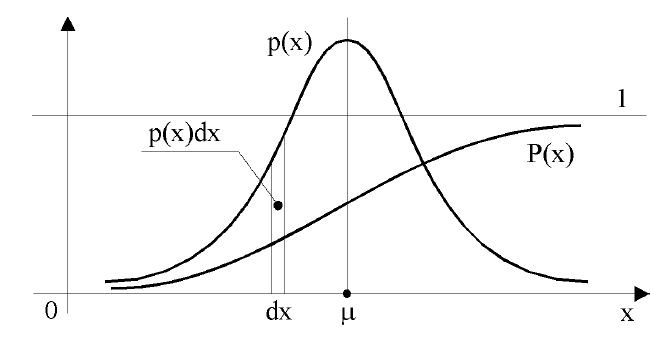
\includegraphics[scale = 0.8]{Curva di Gauss.png}
\end{figure}

\newpage 

\begin{tcolorbox}
    Argomento critico e importante nel corso. \newline

    La GUM, per quanto riguarda le misure, è la bibbia per chi fa misure, 
    quindi se non sai questo capitolo, meglio non svolgere l'esame in generale. \newline 
    
    La norma che andiamo a studiare è da 15 anni circa in vigore, 
    ma, adesso è in revisione. \newline 

    L'importante, anche durante l'esame scritto, sono i passaggi matematici che si svolgono. 
\end{tcolorbox}

\section{Regole di scrittura delle unità di misura}
\footnote{Slide della prof | SDME 2 Incertezza secondo GUM parte I | pag 2 - 4 \\  
Appunti | 2025-03-05 | pag 2 - 3}

Per questioni di praticità, sono stati introdotti i multipli ed i sottomultipli decimali delle unità di misura 
dell'SI, che si ottengono utilizzando i seguenti prefissi: 

\begin{figure}[h]
    \centering
    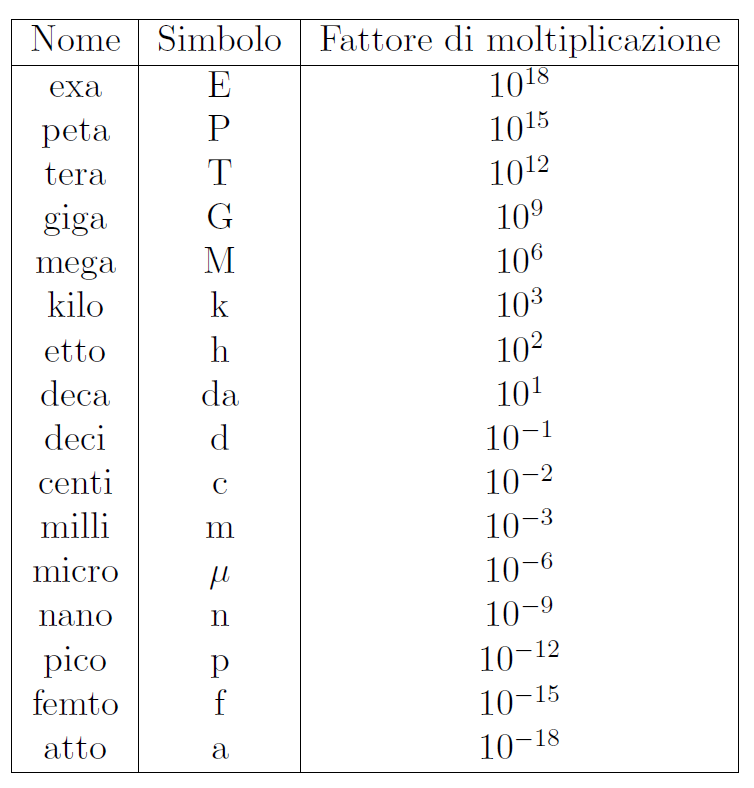
\includegraphics[scale = 0.5]{Tabella mutlipli e sottomultipli.png}
\end{figure}

Il simbolo di un multiplo o di un sottomultiplo di un'unità di misura 
si forma anteponendo il prefisso al simbolo dell'unità di misura. \newline 

Ad esempio: 

\begin{figure}[h]
    \centering
    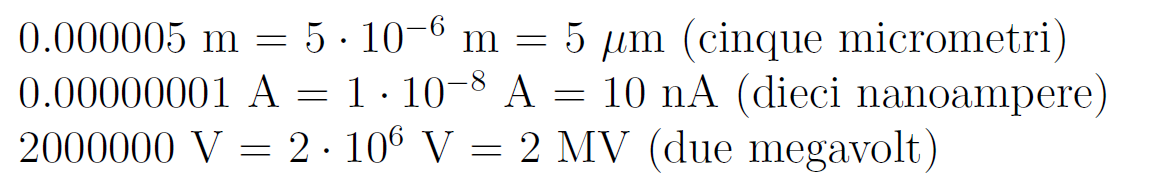
\includegraphics[scale = 0.3]{Esempi di conversione secondo GUM.png}
\end{figure}

Non è ammesso l'uso di prefissi composti, ad esempio: 

{
    \Large 
    \begin{equation}
        5 \text{ } pF \neq 5 \text{ } mnF
    \end{equation}
}

Prendendo come esempio l'u.d.m. del peso, cioè il grammo (g), 
i multipli ed i sottomultipli dell'unità fondamentale kilogrammo si formano a partire dal simbolo grammo. \newline 

Per esempio, si scrive: 

{
    \Large 
    \begin{equation}
        1 \text{ } mg \textbf{ NON } 1 \mu kg
    \end{equation}
}

Quando si fornisce il risultato di una misurazione, 
devono essere riportate soltanto le cifre significative, 
per cui è opportuno ricorrere ai multipli e sottomultipli delle unità SI per evitare ambiguità. \newline 

Nella seguente tabella, ci sono degli esempi: 

\begin{figure}[h]
    \centering
    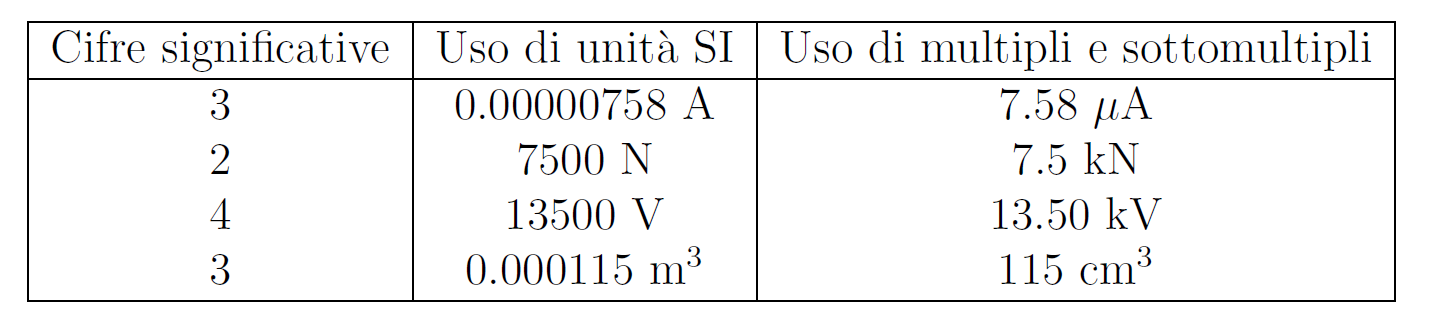
\includegraphics[scale = 0.3]{Esempio di cifre significative.png}
\end{figure}

I nomi delle unità SI, dei multipli e dei sottomultipli sono nomi comuni, 
per cui devono essere scritti con l'iniziale minuscola. \newline 

Si scriverà: 

\begin{itemize}
    \item ampere NON Ampere 
    \item kelvin NON Kelvin 
    \item gigahertz NON Gigahertz 
    \item gigahertz NON GigaHertz
\end{itemize}

Anche i simboli delle unità di misura sono scritti con l'iniziale minuscola, 
tranne quelli derivanti da nomi propri. \newline 

Quindi si scrivere: 

\begin{itemize}
    \item s per secondo 
    \item m per metro 
    \item C per coulomb 
    \item J per joule 
\end{itemize}

I nomi di tutte le unità SI e dei corrispondenti multipli e sottomultipli sono invariabili 
al plurale, eccetto per il metro, il kilogrammo, il secondo, la candela, la mola, il radiante e lo steradiante. \newline 

Il radiante e lo steradiante vengono utilizzati per esprimere i piani di una sfera. \newline 

Quindi è corretto scrivere: 

\begin{itemize}
    \item decine di metri 
    \item centinaia di volt, NON centinaia di volts 
    \item alcuni radianti 
    \item pochi kelvin, NON pochi kelvins
\end{itemize}

I simboli delle unità di misura devono essere scritti in carattere dritto normale, 
non devono essere seguiti da punti, tranne il caso in cui si trovano alla fine di un periodo, 
e devono seguire sulla stessa linea il valore numero che esprime la misura. \newline 

Quindi, è corretto $7.5$ V e NON V $7.5$. \newline 

Quando un'unità non accompagna la relativa misura, 
deve essere espressa con il suo nome e non con il suo simbolo. \newline 

Si scrive: 

\begin{itemize}
    \item il secondo è la durata NON il s è la durata 
    \item una lunghezza di alcuni metri e NON una lunghezza di alcuni m
\end{itemize}

I simboli di un'unità derivata ottenuta dal prodotto di due o più unità fondamentali
si indica interponendo il punto di moltiplicazione o uno spazio tra i simboli delle unità fondamentali. \newline 

Si scrive, ad esempio, 
N $\cdot$ m oppure N m .\newline 

Nel caso di unità derivate ottenute dal rapporto tra unità fondamentali, 
il simbolo dell'unità derivata si indica interponendo tra i simboli a numeratore e quelli a denominatore 
la barra obliqua o la riga di frazione. \newline 

In alternativa, possono essere usati gli esponenti negativi. \newline 

Si scrive, ad esempio J/s, m $\cdot$ $s^{-1}$. \newline 

\newpage 

\section{Unità non SI ammesse}
\footnote{Slide della prof | SDME 2 Incertezza secondo GUM parte I | pag 5 \\  
Appunti | 2025-03-05 | pag 3}

Alcune unità di misura non SI sono, per ragioni storiche, largamente utilizzate in campo scientifico, 
tecnico, commerciale e nella vita comune. \newline 

L'uso di queste unità è ammesso, MA non incoraggiato; 
inoltre, è sconsigliato associare unità SI e unità non SI. \newline 

La seguente tabella riporta alcune delle unità non SI ammesse: 

\begin{figure}[h]
    \centering
    \includegraphics[scale = 0.3]{Alcune unità non SI ammesse.png}
\end{figure}

\newpage 

\section{Il processo reale di misurazione e la definizione di "Misura"}
\footnote{Slide della prof | SDME 2 Incertezza secondo GUM parte I | pag 6 \\  
Appunti | 2025-03-05 | pag 3}

La definizione di misura data dalla norma UNI 4546 è una informazione costituita 
da un valore, una incertezza ed una unità di misura, segnata a rappresentare un parametro in un determinato stato del sistema. \newline 

Degli esempi di misure: 

\begin{figure}[h]
    \centering
    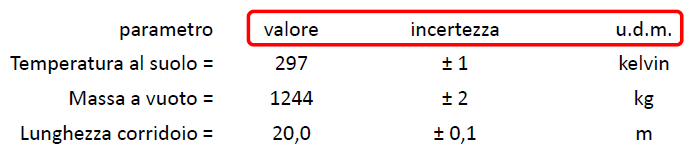
\includegraphics[scale = 0.5]{Esempi di misure.PNG}
\end{figure}

\newpage 

\section{La norma internazionale}
\footnote{Slide della prof | SDME 2 Incertezza secondo GUM parte I | pag 7 - 8 \\  
Appunti | 2025-03-05 | pag 4}

L'incertezza del risultato di una misurazione costituisce la mancanza di una conoscenza esatta del misurando. \newline 

Così, il risultato di una misurazione, quand'anche riuscissimo a correggere effetti sistematici identificati, 
costituisce sempre una stima del valore del misurando. \newline 

Il valore centrale è quello che noi scegliamo, indicando il suo intervallo perché 
il "valore vero" starà nell'intervallo. \newline 

L'incertezza sperimentale è dovuta a numerosi fattori, tra i quali: 

\begin{itemize}
    \item Definizione incompleta del misurando, imperfetta realizzazione del misurando 
    \item Distorsione personale dell'operatore nella lettura di strumenti analogici 
    \item Valori non esatti dei campioni e dei materiali di riferimento
\end{itemize}

Tutti questi fattori, inoltre, non sono sempre indipendenti, ma, 
in questo corso, li consideriamo indipendenti perché i calcoli sono molto più semplici. \newline 

Per questi fattori che possono "disturbare" la misura, anche se la GUM è breve, 
diventa molto più lunga a causa delle appendici con tutti i casi particolari. \newline 

\newpage 

\section{Approccio classico Vs GUM}
\footnote{Slide della prof | SDME 2 Incertezza secondo GUM parte I | pag 9 \\  
Appunti | 2025-03-05 | pag 5}

Analizzeremo la differenza tra errore, che è l'approccio classico, e l'incertezza, che è l'approccio della GUM. \newline 

Quando si parla di incertezza, ci si riferisce alla sola componente casuale. \newline 

Si dà per scontato che, se si mette in evidenza un effetto sistematico, 
questo vada corretto \textbf{PRIMA} di effettuare delle misure, e tale correzione sarà affetta anch'essa da una incertezza. \newline 

Nell'approccio classico, ci si riferisce all'origine dell'incertezza, 
mentre la divisione data nella GUM riguarda i metodi di valutazione dell'incertezza. \newline 

\newpage 

\section{Incertezza: altre considerazioni}
\footnote{Slide della prof | SDME 2 Incertezza secondo GUM parte I | pag 10 \\  
Appunti | 2025-03-05 | pag 5}

Alcune note riguardando l'incertezza. \newline 

Solo le definizioni hanno incertezza nulla. \newline 

C'è una incertezza intrinseca, la quale è la minima incertezza che può essere assegnata nella misura di un parametro, 
fissato un modello descrittivo della grandezza. \newline 

Spesso le prestazioni degli strumenti e dei campioni sono esuberanti rispetto ai requisiti necessari per la misura. \newline 

\newpage 

\subsection{Categorie di incertezza}
\footnote{Slide della prof | SDME 2 Incertezza secondo GUM parte I | pag 11 - 13 \\  
Appunti | 2025-03-05 | pag 5 - 6 | 2025-03-07 | pag 2}

La GUM classifica le componenti di incertezza in due categorie, 
in relazione al metodo di valutazione: 

\begin{itemize}
    \item Componenti valutate con metodi statistici (detti di tipo A), sono incertezze di misura che sono basati su metodi statistici, quindi oggettivi, perché la misura può essere ripetuta 
    \item Componenti valutate con altri metodi (detti di tipo B): si svolgerà una valutazione di tipo soggettivo perché la misura non può essere ripetuta
\end{itemize}

La regola di base è quella di fare, se possibile, almeno 3 misure. \newline 

La classificazione non indica alcuna differenza tra la natura delle componenti di incertezza. \newline 

I componenti di tipo B, generalmente, vengono basati sulla "bravura" dell'operatore. \newline 

È importante sottolineare che se il numero di ripetizioni della misura è relativamente ridotto, si fa più affidamento all'incertezza di tipo B. \newline 

Sia nelle categoria di tipo A e di tipo B, l'incertezza è valutata tramite una distribuzione di probabilità e la relativa deviazione standard. \newline 

Il principio base dell'approccio della GUM è che ogni componente di incertezza che contribuisce all'incertezza 
del risultato di misura è rappresentabile dalla stima del suo scarto tipo, 
chiamata incertezza tipo (che è indicata con la lettera u dall'inglese uncertainty) ed è uguale alla radice quadrata positiva della stima della varianza. 

\begin{tcolorbox}
    Tranquilli, nelle prossime sezioni sarà spiegato meglio con delle formule matematiche
\end{tcolorbox}

Se durante la misura tutte le grandezze d'influenza da cui essa dipende variano in modo casuale, 
si può utilizzare un approccio di tipo statistico, quindi di tipo A. \newline 

In diversi casi, ripetere le misure è una operazione lunga e costosa, non sempre fattibile. \newline 

Quindi, l'incertezza finale sulla misurazione è ottenuta sia dall'incertezza di tipo A e di tipo B. \newline 

\newpage 

\section{Alcuni richiami di statistica e probabilità}
\footnote{Slide della prof | SDME 2 Incertezza secondo GUM parte I | pag 14 - 16 \\  
Appunti | 2025-03-05 | pag 6 - 10 | 2025 -03-07 | pag 3}

\begin{tcolorbox}
    Sono gli stessi concetti di probabilità studiati a Teoria dei Segnali / Segnali Determinati Aleatori con il mitico Chiaraluce 
    ma applicati e adattati alla teoria delle misure
\end{tcolorbox}

Prendiamo in considerazione un indice quadratico, la varianza. \newline 

Definiamo varianza sperimentale dell'insieme di N misure il valore medio del quadrato delle deviazioni: 

{
    \Large 
    \begin{equation}
        \begin{split}
            s^{2} (x_k) 
            &= 
            \frac{1}{N - 1}
            \sum_{k = 1}^{N}
            \delta^{2}_k
            \\
            &= 
            \frac{1}{N - 1}
            \sum_{k = 1}^{N}
            (x_k - \overline{x})^{2}
        \end{split}
    \end{equation}
}

dove: 

\begin{itemize}
    \item $\overline{x}$ è la media dei valori 
    \item $x_k$ è il singolo valore della misura
\end{itemize}

Si pone $(x_k - \overline{x})^{2}$ elevato alla seconda perché $\delta_k$ può essere sia positivo che negativo. \newline

Da questa varianza, si deduce lo scarto tipico sperimentale come: 

{
    \Large 
    \begin{equation}
        \begin{split}
            s(x_k) 
            &=
            \sqrt
            { 
            \frac{1}{N - 1}
            \sum_{k = 1}^{N}
            \delta^{2}_k
            }
            \\
            &= 
            \sqrt
            {
            \frac{1}{N - 1}
            \sum_{k = 1}^{N}
            (x_k - \overline{x})^{2}
            }
        \end{split}
    \end{equation}
}

\newpage

\subsection{Scarto di tipo sperimentale}
\footnote{Slide della prof | SDME 2 Incertezza secondo GUM parte I | pag 17 \\  
Appunti | 2025-03-07 | pag 3 - 4}

Lo scarto tipo o deviazione standard rappresenta un indice appropriato della dispersione delle misure intorno al valore medio. \newline 

La sua definizione sarà, tuttavia, affinata, in seguito considerando che le N misure non rappresentano l'insieme (cioè la popolazione) di tutte 
le misure, 
ma solo un campione limitato dell'infinità di misure (teoricamente) eseguibili. \newline 

Utilizzando i diagrammi di Venn, possiamo rappresentare il caso della misura come:


%è la prima volta che provo a fare i disegni, sto seguendo questa guida: 
%https://latexdraw.com/how-to-draw-venn-diagrams-in-latex/

%E come al solito, Reddit salva la gente: 
%https://www.reddit.com/r/LaTeX/comments/o2367s/how_do_i_horizontally_centre_a_tikz_diagram/

% Circle with label
{
    \begin{center}
        \begin{tikzpicture}
    
            \node[draw,
                circle,
                minimum size =4cm,
                fill=red!50,
                label=$Popolazione$] (circle1) at (0,0){};
            
            \node[draw, 
                circle, 
                minimum size = 1cm, 
                fill =blue!50, 
                label = $Campione$] (circle2) at (0,0) {};    
             
            \end{tikzpicture}    
    \end{center}
    
}

dove: 

\begin{itemize}
    \item nell'insieme della popolazione ci dovrebbero essere infiniti elementi 
    \item nell'insieme campione ci sono N elementi, quelli della misura
\end{itemize}

Quindi dagli elementi statistici utilizzati, e che hai imparato a conoscere al corso di teoria dei segnali con il mitico Chiaraluce, come: 

\begin{itemize}
    \item media $\mu$ 
    \item scarto (deviazione standard) $\sigma$
\end{itemize}

in una misura di N elementi utilizzeremo: 

\begin{itemize}
    \item media sperimentale $\overline{x}$ al posto di $\mu$ 
    \item deviazione scarto sperimentale $s(x_k)$ al posto di $\sigma$
\end{itemize}

\newpage 

\section{Istogrammi delle osservazioni}
\footnote{Slide della prof | SDME 2 Incertezza secondo GUM parte I | pag 18 - 21 \\  
Appunti | 2025-03-07 | pag 5}

Il risultato di numerose misure ripetute N sulla stessa grandezza 
possono essere graficamente rappresentati in opportuni diagrammi, 
detti istogrammi delle osservazioni come il seguente grafico: 

\begin{figure}[h]
    \centering
    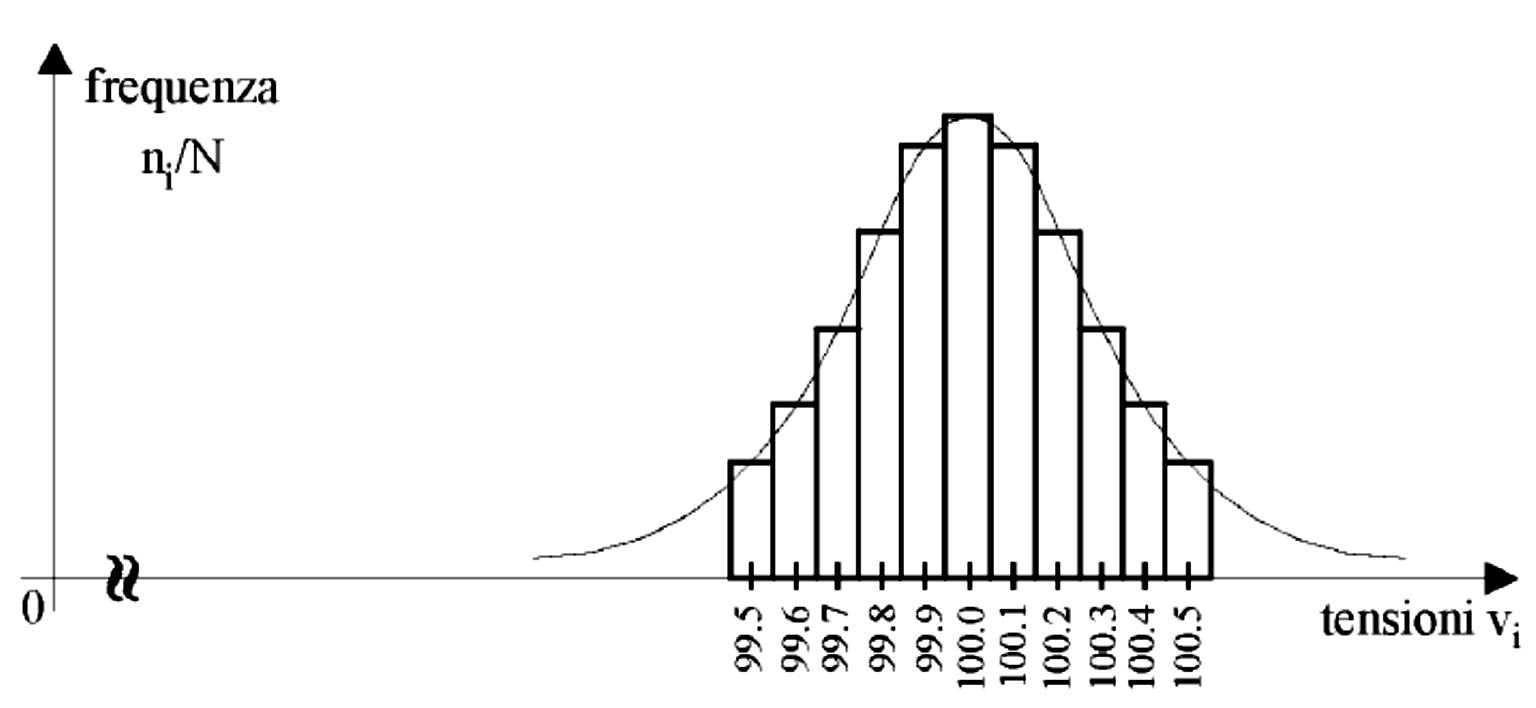
\includegraphics[scale = 0.2]{Esempio di istogramma delle osservazioni.png}
\end{figure}

Questi si costruiscono con alcune semplici operazioni: 

\begin{enumerate}
    \item Si individuano i valori massimo ($x_{max}$) e minimo ($x_{min}$) tra le N misure della grandezza X 
    \item Si divide l'intervallo ($x_{max} - x_{min}$) in un numero M di sotto-intervalli (chiamati in inglese bins) di uguale ampiezza, ciascuno dei quali può essere identificato col suo valore centrale \\ $x_i$ (i = 1, ..., M) 
    \item Si conta il numero $n_i$ delle misure che ricadono in ciascun sotto-intervallo 
    \item Si calcola la frequenza di osservazione dividendo questo numero per il numero totale delle osservazioni N: 
    {
        \Large 
        \begin{equation}
            f_i = \frac{n_i}{N} \text{ } (i = 1, 2, .., M)
        \end{equation}
    } 
    e, dalla teoria della probabilità: 

    {
        \Large 
        \begin{equation}
            \sum_{i=1}^{M}
            f_i 
            = 
            1
        \end{equation}
    }
\end{enumerate}

$f_i$ è la definizione frequentistica di probabilità. \newline 

Inoltre, la figura non è solo un istogramma, 
ma è un insieme tra istogramma, che è una funzione discreta, 
e una funzione normale continua, che è una astrazione matematica. \newline 
 
\newpage 

\section{Alcuni richiami di statistica e probabilità}
\footnote{Slide della prof | SDME 2 Incertezza secondo GUM parte I | pag 22 \\  
Appunti | 2025-03-07 | pag 6}

Con riferimento alle frequenze $f_i$, il valore medio è: 

{
    \Large 
    \begin{equation}
        \begin{split}
        \overline{x}
        &= 
        \frac{1}{N}
        \sum_{k = 1}^{N}
        x_k 
        \\
        &=
        \sum_{i = 1}^{M}
        x_i 
        \frac{n_i}{N} 
        \\ 
        &= 
        \sum_{i = 1}^{M}
        x_i f_i
        \end{split}
    \end{equation}
}

Invece la varianza si può scrivere come: 

{
    \Large 
    \begin{equation}
        \begin{split}
            s^{2} (x_i) 
            &= 
            \frac{1}{N - 1}
            \sum_{k = 1}^{N}
            \delta^{2}_k
            \\ 
            &= 
            \sum_{i = 1}^{M} 
            \delta^{2}_i 
            \frac{n_i}{N - 1}
            \\ 
            &= 
            \sum_{i = 1}^{M} 
            \delta^{2}_i 
            f^{\sim}_i
        \end{split}
    \end{equation}
}

in cui: 

{
    \Large 
    \begin{equation}
        \delta_i = x_i - \overline{x}
    \end{equation}
}

è lo scostamento della i-esima classe rispetto al valore medio. \newline 

M è il numero di valori distinti delle misure (cioè il numero di bins, dall'inglese "cestini"). \newline 

\newpage 

\section{Il concetto di probabilità ed i parametri statistici}
\footnote{Slide della prof | SDME 2 Incertezza secondo GUM parte I | pag 23 \\  
Appunti | 2025-03-07 | pag 6}

Se fosse possibile effettuare sulla stessa grandezza fisica X 
un numero N di misure infinitamente grande, 
le frequenze di occorrenza dei diversi valori rappresentano le probabilità dell'intera popolazione. \newline 

L'insieme delle misure può essere visto come una variabile aleatoria discreta X, 
dove ciascuno dei possibili valori $x_i$ è caratterizzato dalla sua probabilità di occorrenza: 

{
    \Large 
    \begin{equation}
        \begin{split}
            Prob(x_i)
            &= 
            P(x_i) 
            \\ 
            &=
            P_i 
            \\ 
            &= 
            \lim_{N \to \infty} 
            \frac{n_i}{N}
        \end{split}
    \end{equation}
}

Essendo un limite che tende ad infinito, nella realtà non si possono fare infinite misure: 
ecco perché viene utilizzata la statistica. \newline 

Molti fenomeni fisici, interessati solo da disturbi casuali, se osservati un numero di volte molto grande, 
obbediscono a una legge di occorrenza degli eventi detta Gaussiana o Normale. \newline 

\newpage 

\section{Curva normale o di Gauss}
\footnote{Slide della prof | SDME 2 Incertezza secondo GUM parte I | pag 24 \\  
Appunti | 2025-03-07 | pag 6}

Un esempio di curva normale o di Gauss: 

\begin{figure}[h]
    \centering
    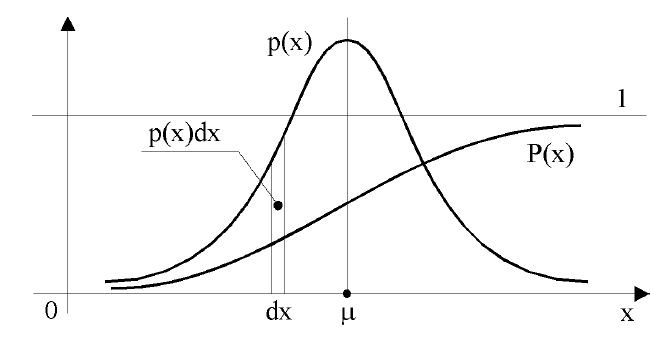
\includegraphics[scale = 0.4]{Curva di Gauss.png}
\end{figure}

Il diagramma della curva Normale o di Gauss per una variabile aleatoria continua X 
riporta in ascisse i possibili valori continui x della variabili aleatoria, 
mentre in ordinate si riporta la densità di probabilità p(x) con cui si osservano tali valori, 
e la probabilità cumulativa P(x). \newline 

\newpage

\section{Distribuzioni di probabilità}
\footnote{Slide della prof | SDME 2 Incertezza secondo GUM parte I | pag 25 - 27 \\  
Appunti | 2025-03-07 | pag 6 - 9}

La densità di probabilità p(x) è, in generale, quella funzione continua che, 
moltiplicata per una variazione infinitesima dx, fornisce la probabilità della variabile aleatoria X 
che cada dentro l'intervallo dx. \newline 

Quindi: 

{ 
    \Large 
    \begin{equation}
        Prob[x \leq X \leq (x + dx)]
        = 
        p(x) dx
    \end{equation}
}

La probabilità cumulativa P(x) è la probabilità che la variabile aleatoria X sia minore del valore corrente x: 

{
    \Large 
    \begin{equation}
        \begin{split}
            Prob [X < x]
            &= 
            P(x) 
            \\ 
            &= 
            \int_{- \infty}^{x}
            p(z) 
            dz 
        \end{split}
    \end{equation}
}

allora: 

{
    \Large 
    \begin{equation}
        \int_{- \infty}^{+ \infty} 
        p(x) dx 
        =
        1 
    \end{equation}
}

Invece si definisce valore medio come: 

{
    \Large 
    \begin{equation}
        \mu = \int_{- \infty}^{+ \infty} x \cdot p(x) dx
    \end{equation}
}

Si definisce varianza come: 

{
    \Large 
    \begin{equation}
        \sigma^{2}
        = 
        \int_{- \infty}^{+ \infty} 
        (x - \mu)^{2} \cdot p(x) dx
    \end{equation}
}

La radice quadrata della varianza è definita come scarto tipo o deviazione standard $\sigma$. \newline 

Talvolta, la densità di probabilità p(x) è riferita, anziché ai valori x delle misure, 
alle loro deviazioni $\delta = (x - \mu)$, tramite una semplice traslazione pari al valore medio. \newline 

Nella teoria della statistica, la gaussiana normale, quindi la gaussiana con area = 1, 
è molto utile per i calcoli, in particolare nelle misure può essere utilizzata per dimostrare la bontà della misura svolta. \newline 

Di seguito la densità di probabilità delle deviazioni standard normalizzata, la quale è diversa dalla densità di probabilità non normalizzata (perché l'area della funzione non è unitaria): 

\begin{figure}[h]
    \centering
    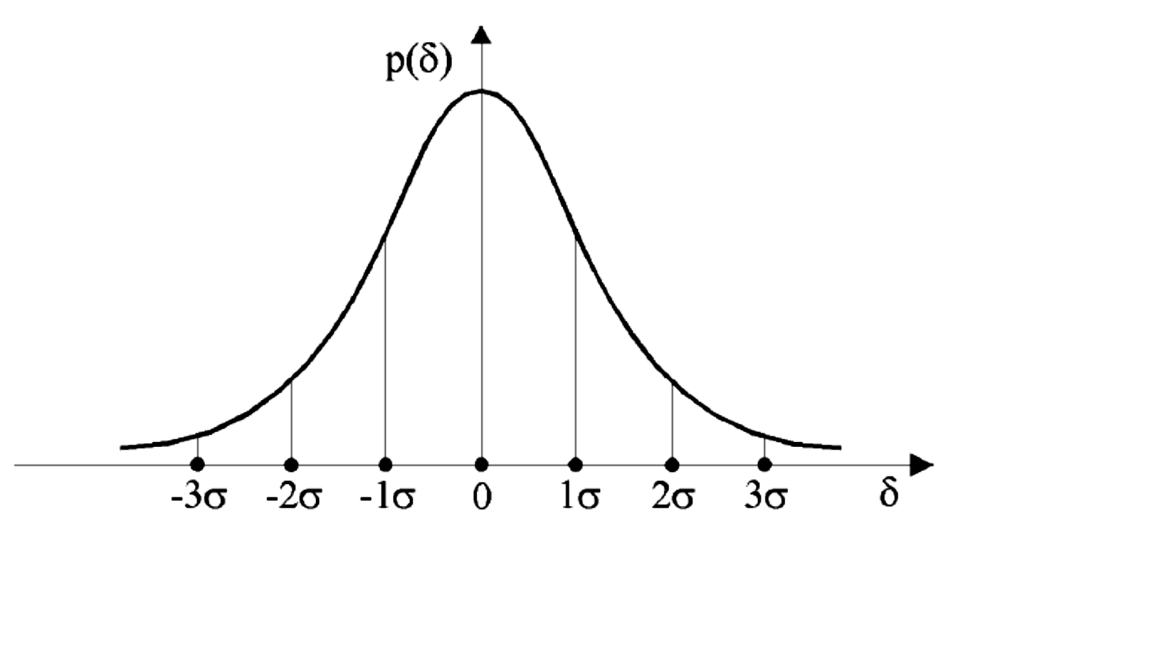
\includegraphics[scale = 0.4]{curva standard normalizzata di gaus.png}
\end{figure}

\newpage 

Si utilizza proprio una distribuzione di Gauss perché, da Segnali Determinati con Chiaraluce, 
il rumore ha questa distribuzione perché è un fenomeno stocastico. \newline 

Nella teoria delle misure e nella statistica, si divide la funzione gaussiana in $\sigma$ e suoi multipli. \newline 

Di seguito la relazione tra $\sigma$ e percentuale: 

{
    \Large 
    \begin{equation}
        Prob[- \sigma \leq \Delta \leq + \sigma] = 68.27 \%
    \end{equation}
}

{
    \Large 
    \begin{equation}
        Prob[- 2 \sigma \leq \Delta \leq + 2 \sigma] = 95.45 \%
    \end{equation}
}

{
    \Large 
    \begin{equation}
        Prob[- 3 \sigma \leq \Delta  \leq + 3 \sigma] = 99.73 \%
    \end{equation}
}


Assumendo l'intervallo $\pm 3 \sigma$ si avrà 99.73 \% che è circa 100 \% . \newline 

La bontà delle misure dipende dal suo scarto tipo: 
più è piccolo, meglio è perché la campana della gaussiana è più stretta. \newline 

Confrontando, ad esempio due misure di due laboratori: 

\begin{figure}[h]
    \centering
    \includegraphics[scale = 0.6]{Esempio bontà di misure.PNG}
\end{figure}

Le misure del laboratorio 1 sono di maggiori qualità rispetto al laboratorio 2 perché, 
riportando le densità di probabilità nelle distribuzioni normalizzate gaussiane, 
ci saranno più valori del laboratorio 1 rispetto alle misure del secondo laboratorio. \newline 

Per concludere, la densità di probabilità è un modello matematico, quindi non applicabile nella realtà perché N tende 
all'infinito, quindi useremo $s_k$ e i valori sperimentali. \newline 

\newpage 





\chapter{Valutazione dell'incertezza di tipo A e B}

\begin{figure}[h]
    \centering
    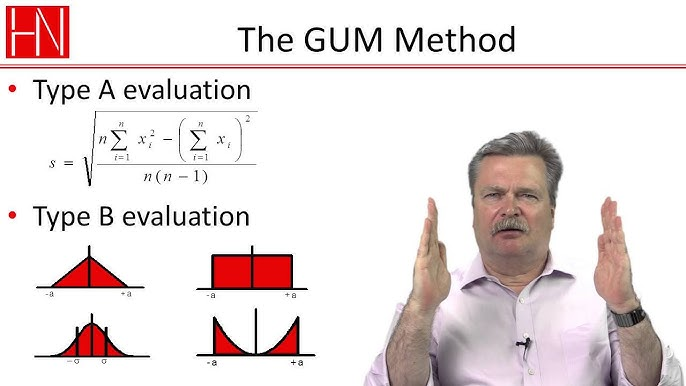
\includegraphics[scale = 0.5]{Video del bro.jpg}
\end{figure}

\newpage 

\section{Valutazione dell'incertezza}
\footnote{Slide della prof | SDME 2 Incertezza secondo GUM parte II | pag 2 - 5 \\  
Appunti | 2025-03-07 | pag 10 - 11}

Come scritto precedentemente, il problema che si pone nella misura è quello di "riportare" gli strumenti utilizzati in statistica 
in una popolazione con infiniti elementi all'insieme delle misure con elementi finiti. \newline 

Quindi dobbiamo discutere delle stime dei parametri da campioni e non dalla popolazione. \newline 

Si utilizza il valore medio sperimentale $\overline{x}$ perché è la stima migliore del valore atteso della media $\mu$ della popolazione: 
si dice che $\overline{x}$ è il miglior stimatore corretto e consistente di $\mu$. \newline 

\begin{tcolorbox}
    Il concetto di stimatore corretto e consistente non viene approfondito in questo corso, lo diamo per buono
\end{tcolorbox}


Per quanto riguarda lo scarto tipo $\sigma$ della popolazione, 
si parte dall'espressione dello scarto tipo sperimentale: 

{
    \Large 
    \begin{equation}
        s(x_k)
        = 
        \sqrt
        {
            \frac{1}{N-1} \sum_{k = 1}^{N} 
            (x_k - \overline{x})^{2}
        }
    \end{equation}
}

La deviazione standard sperimentale $s(x_k)$ rappresenta il grado di attendibilità della generica misura $x_k$ 
fra le N del campione o, in altri termini, quantifica la dispersione degli N valori misurato attorno al loro valore medio $\overline{x}$. \newline 

Graficando K serie di misura: 

\begin{figure}[h]
    \centering
    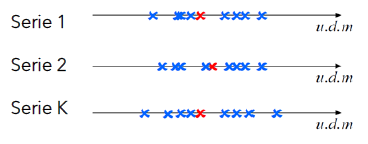
\includegraphics[scale = 0.8]{Esempi di serie di misure.PNG}
\end{figure}

si può notare che, in ogni singola serie di misura, quella indicata con la x blu è il risultato della singola misura, 
invece la x in rosso indica il valore medio della singola serie. \newline 

Mettendo le serie insieme, si può calcolare e determinare la dispersione dei valori medi sperimentali (cioè la dispersione delle x rosse). \newline 

Si dimostra (cioè non lo dimostriamo, prendiamolo per buono) che la varianza del valore medio sperimentale fra i vari gruppi di N misure, 
è esprimibile nel seguente modo: 

{
    \Large 
    \begin{equation}
        s^{2} (\overline{x}) 
        = 
        \frac{s^{2} (x_k)}{N}
    \end{equation}
}

allora, con dei semplici passaggi algebrici e sostituzioni: 

{
    \Large 
    \begin{equation}
        \begin{split}
            s(\overline{x})
            &= 
            \frac{s(x_k)}{\sqrt{N}} 
            \\ 
            &= 
            \sqrt
            {
                \frac{1}{N (N-1)}
                \sum_{k = 1}^{N}
                (x_k - \overline{x})^{2}
            }
        \end{split}
    \end{equation}
}

$s(x_k)$ NON è uno stimatore corretto di $\sigma$ e va diviso per $\sqrt{N}$ per diventarlo. \newline 

$s(\overline{x})$, cioè lo scarto tipo del valore medio sperimentale, costituisce una stima della deviazione standard $\sigma$ di tutta la popolazione. \newline 

Quindi useremo: 

\begin{itemize}
    \item $\overline{x}$ al posto di $\mu$ 
    \item $s(\overline{x})$ al posto di $\sigma$
\end{itemize}

\newpage 

\section{Valutazione dell'incertezza di tipo A}
\footnote{Slide della prof | SDME 2 Incertezza secondo GUM parte II | pag 6 \\  
Appunti | 2025-03-07 | pag 12}

La varianza sperimentale della media $s^{2}(\overline{x})$ e lo scarto tipo sperimentale della media $s (\overline{x})$, 
indicano quanto bene $\overline{x}$ stimi il valore medio $\mu$ della popolazione (che sarebbe il valore atteso) e, pertanto, verranno 
adottati come valutazioni quantitative dell'incertezza di $\overline{x}$. \newline 

Diremo quindi che una grandezza fisica X, che è la grandezza sotto misura, determinata con N osservazioni ripetute, 
avrà un'incertezza (uncertainty) sulla stima $\overline{x}$ pari a: 

{
    \Large 
    \begin{equation}
        u^{2} (x) = s^{2} (\overline{x})
    \end{equation}
}

in termini di varianza e 

{
    \Large 
    \begin{equation}
        u(x) = s(\overline{x})
    \end{equation}
}

in termini di scarto tipo. \newline 

Quindi, se avremo a che fare solo con misure di tipo A, 
la misura finale dobbiamo esprimerla come: 

{
    \Large 
    \begin{equation}
        \begin{split}
            X 
            &= 
            \overline{x} \pm u_a (\overline{x}) \text{ } [u.d.m.] 
            \\ 
            &= 
            \overline{x} \pm s (\overline{x}) \text{ } [u.d.m.]  
        \end{split}
    \end{equation}
}

dove: 
\begin{itemize}
    \item X è la grandezza sotto misura
\end{itemize}

\newpage

\section{Valutazione dell'incertezza di tipo B}
\footnote{Slide della prof | SDME 2 Incertezza secondo GUM parte II | pag 7 - 10 \\  
Appunti | 2025-03-07 | pag 12 - 13 | 2025-03-11 | pag 2 - 4}

Adesso passiamo dall'incertezza di tipo A, cioè da misure ripetute, 
all'incertezza di tipo B, cioè una misura da una ripetizione. \newline 

Quando una grandezza X non viene determinata da osservazioni ripetute, 
bensì con una misura singola, 
la varianza stimata $u^{2} (x)$ o lo scarto tipo u(x) sono valutati per mezzo 
di un giudizio scientifico basato su tutte le altre informazioni disponibili: 

\begin{itemize}
    \item dati di misurazioni precedenti 
    \item conoscenza del comportamento e delle proprietà dei materiali e degli strumenti 
    \item specifiche tecniche del costruttore (sono indicate nel manuale dello strumento)
    \item dati forniti in certificato di taratura (quindi dai LAT) 
    \item incertezze assegnate a valori di riferimento presi da manuali 
\end{itemize}

L'uso di tali informazioni, per una valutazione di incertezza di tipo B, 
richiede conoscenza, esperienza e perizia che possono acquisirsi solo con la pratica e col tempo. \newline 

L'analisi statistica sulle misure è un'indagine che viene fatta durante la taratura di uno strumento. \newline 

Il certificato di taratura accompagna il singolo strumento nel suo impiego e chi lo utilizza sa che le indicazioni fornite possono avere 
un'incertezza compresa entro l'intervallo dichiarato sul certificato di taratura, 
con un assegnato livello di confidenza. \newline 

Più spesso, i costruttori di strumentazione assegnano le specifiche di accuratezza con valori numerici valida per tutti gli 
esemplari di un dato modello, e per essi dichiarano semplicemente un intervallo di ampiezza (-a, +a), centrato sul valore letto, 
entro il quale si ritiene che cada il valore del misurando. \newline 

Quando compriamo uno strumento da un produttore, 
il costruttore tara alcuni strumenti del lotto, 
quindi, se vogliamo essere più precisi nella misura, 
dobbiamo tarare il nostro strumento in un LAT. \newline

In tal caso, per poter calcolare il valore dell'incertezza in termini di varianza o di deviazione standard, 
in modo da avere a disposizione un'informazione confrontabile con quella ottenuta con la valutazione di tipo A, 
è necessario ipotizzare la distribuzione di probabilità da considerare all'interno dell'intervallo (-a, +a). \newline 

La distribuzione di probabilità della misura è quella funzione che rappresenta 
la probabilità di ottenere un certo valore x come risultato di una misura, funzione del valore x stesso. \newline 

Nella maggior parte dei casi è prassi comune assumere all'interno dell'intervallo 
(-a, +a) una probabilità uniforme (pdf dall'inglese Probability Density Function) centrata in x, come i figura:

    \begin{center}
    \begin{tikzpicture}
        \begin{axis}[
            clip=false,
            axis lines = left,
            xlabel = \(x\),
            ylabel = {\(pdf(x)\)},
            xmin = -2, xmax = 2,
            ymin = 0, ymax = 1,
            xtick = {-1, 0, 1},
            xticklabels = {$-a$, $0$, $+a$},
            ytick = {0, 0.5},
            yticklabels = {$0$, $\frac{1}{2}$a},
            width=10cm,
            height=6cm,
            domain=-2:2
        ]
        
        % Area evidenziata (distribuzione uniforme)
        \addplot [
            gray!30,
            fill=gray!60,
            opacity=0.3
        ] coordinates {
            (-1,0)
            (-1,0.5)
            (1,0.5)
            (1,0)
        };
    
        % Linea superiore della pdf
        \addplot [
            thick,
            black
        ] coordinates {
            (-1,0.5)
            (1,0.5)
        };
    
        % Linee verticali
        \addplot[thick] coordinates {(-1,0) (-1,0.5)};
        \addplot[thick] coordinates {(1,0) (1,0.5)};
    
        \end{axis}
    \end{tikzpicture}
    \end{center}
    
Considerando z il generico scostante in tale intervallo, si ha:

{
    \Large
    \begin{equation}
        p(z) = \frac{1}{2a}
    \end{equation}
}

p(z) è uguale a $\frac{1}{2a}$ proprio perchè, dall'esame di Teoria dei Segnali, l'area, 
cioè l'integrale della pdf deve essere uguale a uno. \newline 

Sapendo p(z) si può calcolare la varianza della misura x come: 

{
    \Large 
    \begin{equation}
        \begin{split}
            u^{2} (x)
            &= 
            \int_{-a}^{+a} 
            z^{2} p(z) dz 
            \\
            &= 
            \int_{-a}^{+a}
            z^{2} \frac{1}{2a} dz 
            \\ 
            &= 
            \frac{1}{2a} \cdot 
            \left.
                \frac{z^{3}}{3}
            \right|^{+a}_{-a}
            \\
            &= 
            \frac{a^{2}}{3}
        \end{split}
    \end{equation}
} 

Sapendo la relazione tra varianza e incertezza di tipo B, 
l'incertezza assoluta di tipo B associata alla quantità x risulta quindi: 

{
    \Large 
    \begin{equation}
        u(x) = \frac{a}{\sqrt{3}}
    \end{equation}
}


L'ipotesi di distribuzione uniforme è piuttosto pessimistica, ma è anche quella suggerita dalla GUM in mancanza di ulteriori informazioni. \newline 

Se invece possiamo ipotizzare che i valori centrali dell'intervallo [-a, +a] sono più probabili di verificarsi, 
si può assumere una distribuzione di tipo gaussiano, come in figura: 


\begin{figure}[h]
    \centering
    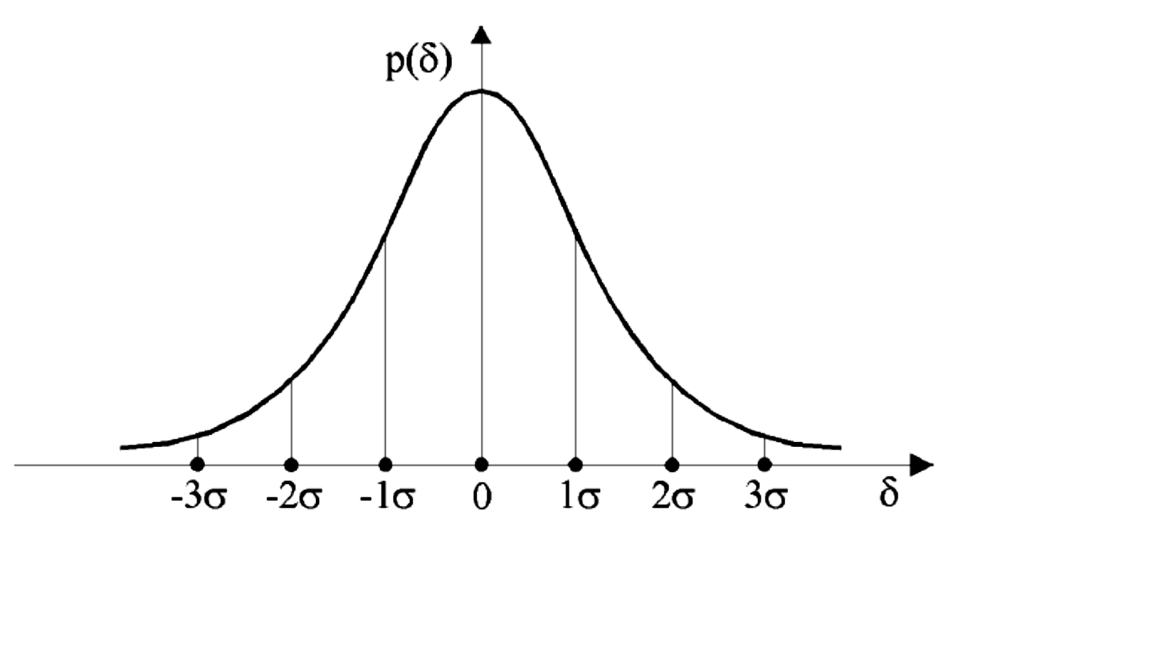
\includegraphics[scale = 0.4]{curva standard normalizzata di gaus.png}
\end{figure}

Se si considera: 

{
    \Large 
    \begin{equation}
        a = 3\sigma
    \end{equation}
}

si svolge il calcolo della varianza come abbiamo svolto per la distribuzione uniforme, 
ma, in questo caso, l'incertezza associata alla quantità x risulta in una distribuzione di tipo gaussiano come: 

{
    \Large
    \begin{equation}
        u(x) = \frac{a}{3}
    \end{equation}
}

Quindi, p(z) con distribuzione gaussiana è quella con l'incertezza più bassa possibile, 
invece p(z) con distribuzione costante è quella con l'incertezza più alta possibile. \newline 

\newpage 

\subsection{Distribuzione triangolare}
\footnote{Slide della prof | SDME 2 Incertezza secondo GUM parte II | pag 11 \\  
Appunti | 2025-03-11 | pag 4 - 5}

Un caso intermedio tra la distribuzione gaussiana e quella uniforme è quella triangolare: 

\begin{figure}[h]
    \centering
    \includegraphics[scale = 0.4]{Distribuzione di probabilità di tipo triangolare.png}
\end{figure}

in cui (tralascio i conti qui, ma il procedimento è lo stesso di prima):

{
    \Large 
    \begin{equation}
        u(x) = \frac{a}{\sqrt{6}}
    \end{equation}
}

\newpage 

\section{Incertezza combinata standard}
\footnote{Slide della prof | SDME 2 Incertezza secondo GUM parte II | pag 20 \\  
Appunti | 2025-03-11 | pag 5}

Quando si vuole svolgere una misura, 
si possono avere due situazioni limite: 

\begin{itemize}
    \item Singola misurazione, non è possibile stimare le incertezze di tipo A, si considerano unicamente quelle di tipo B 
    \item Infinite misurazioni, tutte le grandezze di influenza vengono fatte variare in modo casuale per stimare le cause di incertezza unicamente tramite metodo A
\end{itemize}

Essendo situazioni limite, sono situazioni che sono molto rare: allora, in tutte le misure, ci ritroveremo nel caso intermedio, 
quindi useremo i contributi di incertezza combinata standard. \newline

In genere, i contributi dell'incertezza combinata standard sono ottenuti tramite i metodi A e B contemporaneamente. \newline 



Stimati i contributi sia di tipo A che di tipo B, si passa al calcolo dell'incertezza combinata standard come: 

{
    \Large 
    \begin{equation}
        \begin{split}
        u_c (x)
        &= 
        \sqrt{\sum_{i = 1}^{N} u(x_i)^{2}}
        \\
        &= 
        \sqrt{(u_a (x))^{2} + (u_b (x))^{2} }
        \end{split}
    \end{equation}
}

Di seguito, si può calcolare il valore dell'incertezza estesa U(x) come: 

{ 
    \Large 
    \begin{equation}
        U (x) = k \cdot u_c (x)
    \end{equation}
}

dove k è il fattore di copertura che è un numero scelto intero, 
che tipicamente è compreso tra 1 e 3. \newline 

\newpage 

\section{Incertezza estesa}
\footnote{Slide della prof | SDME 2 Incertezza secondo GUM parte II | pag 18 - 19 \\  
Appunti | 2025-03-11 | pag 5 - 6}

L'incertezza composta $u_c (y)$ viene universalmente accettata per esprimere l'incertezza di una misurazione. \newline 

Normalmente, tuttavia, si richiede che la valutazione quantitativa dell'incertezza venga data come un intervallo U intorno al risultato della misurazione, 
che comprenda "ragionevoli" valori del misurando. \newline 

Da un punto di vista grafico, possiamo vedere il tutto come: 

\begin{figure}[h]
    \centering
    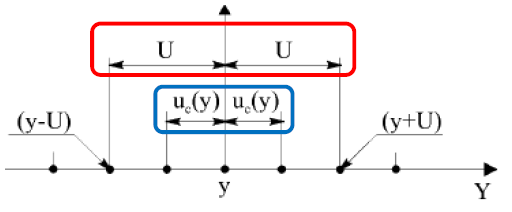
\includegraphics[scale = 0.6]{Incertezza estesa con note.PNG}
\end{figure}

Tale intervallo è denominato come incertezza estesa, 
e si ottiene moltiplicando l'incertezza composta $u_c (y)$ per un fattore di copertura. \newline 

In formule: 

{
    \Large 
    \begin{equation}
        U = k \cdot u_c (y)
    \end{equation}
}

Il fattore di copertura k viene scelto in base al livello di fiducia p che viene 
richiesto all'intervallo [(y - U) ÷ (y + U)]. \newline 

Il livello di fiducia p rappresenta la probabilità di copertura di questo intervallo, 
cioè la probabilità che il risultato dichiarato casa entro l'intervallo [(y - U) ÷ (y + U)]. \newline 

Il legame fra k e p può essere stabilito se sono note le distribuzioni di probabilità 
che caratterizzano i risultati della misurazioni. \newline 

In genere, quindi, non è facile determinare un legame rigoroso. \newline 

Nella pratica, si può ritenere che: 

\begin{itemize}
    \item k = 2, corrisponda a un livello di fiducia di circa il 95 \% 
    \item k = 3, corrisponda a un livello di fiducia di circa il 99 \%
\end{itemize}

\newpage 

\section{Combinazione delle incertezze}
\footnote{Slide della prof | SDME 2 Incertezza secondo GUM parte II | pag 12 - 17 \\  
Appunti | 2025-03-11 | pag 7 - 9}

La GUM si basa su principi lineari e distribuzioni gaussiane, ma, se il fenomeno non lo è, 
la GUM offre degli appendici riguardo al caso non lineare e/o con distribuzioni non gaussiane. \newline 

In questo corso, ci concentriamo solo su principi lineari e distribuzioni gaussiane. \newline 

La definizione dello scarto tipo o della varianza si rivela particolarmente utile nell'analisi 
della combinazione delle incertezze di più fenomeni aleatori, 
cioè nella valutazione dell'incertezza di quantità determinate in modo indiretto: 

{ 
    \Large 
    \begin{equation}
        y = f(x_1, x_2, ..., x_m)
    \end{equation}
}

dove $x_i \text{ } (i = 1, ..., m)$ viene considerata una variabile aleatoria di una grandezza indipendente. \newline 

Si dimostra (cioè non lo dimostriamo) che, se le variabili aleatorie sono tutte fra loro statisticamente indipendenti, 
l'incertezza stimata sulla determinazione indiretta della quantità y, risulta: 

{
    \Large 
    \begin{equation}
        u_c (y) = \sqrt{\sum_{i = 1}^{m} \left[ \left( \frac{\partial f}{\partial x_i} \right) ^{2} u^{2} (x_i)\right]}
    \end{equation}
}

dove 

\begin{itemize}
    \item $u_c (y)$ è l'incertezza tipo composta associata alla grandezza y 
    \item $\frac{\partial f}{\partial x_i}$ è chiamato coefficiente di sensibilità
\end{itemize}

\begin{tcolorbox}
    La frazione $\frac{\partial f}{\partial x_i}$ può, inizialmente, far paura; la si può vedere in questa maniera: \\
    essendo f una funzione di m variabili, fare la derivata parziale della grandezza $x_i$ è come esprimere quanto influisce la grandezza $x_i$ su tutte le altre m-1 grandezze 
    se le m-1 grandezze rimangono costanti
\end{tcolorbox}

Inoltre, in presenza di correlazione fra le variabili di ingresso, 
$u_c (y)$ si può esprimere come: 

{
    \Large 
    \begin{equation}
        u_c (y) = \sqrt{\sum_{i = 1}^{m} \left[ \left( \frac{\partial f}{\partial x_i} \right) ^{2} u^{2} (x_i)\right]
        2 \sum_{i=1}^{m-1} \sum_{j = i+1}^{m}
        \frac{\partial f}{\partial x_i}
        \frac{\partial f}{\partial x_j}
        cov (x_i, x_j)        
        }        
    \end{equation}
}

dove con $cov(x_i, x_j)$ rappresenta la covarianza tra le due variabili e quindi della loro mutua indipendenza. \newline 

La covarianza $cov(x_i, x_j)$ può essere sia positiva che negativa, quindi può comportare sia incrementi che riduzioni dell'incertezza composta $u_c (y)$. \newline 

\begin{tcolorbox}
    Questa ultima formula di $u_c (y)$ NON la useremo mai nel corso perchè, dalla Teoria dei segnali, confideremo le grandezze statisticamente indipendenti, 
    quindi la $cov (x_i, x_j)  = 0$. \newline 

    Perché ho scritto questa formula? Perché la prof ha detto a lezione che la dobbiamo sapere. Fine
\end{tcolorbox}

Di seguito, delle tabelle riassuntive per le leggi di propagazione per legami funzionali semplici: 

\begin{figure}[h]
    \centering
    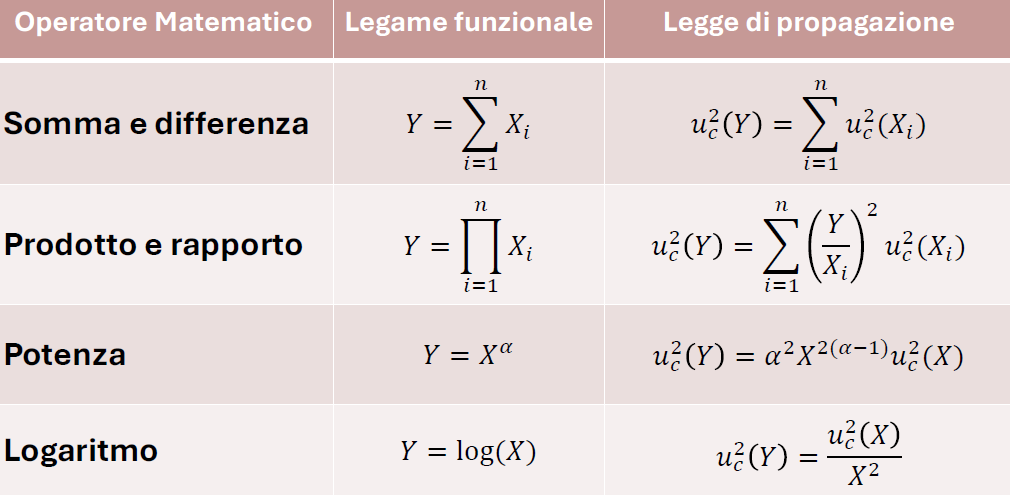
\includegraphics[scale = 0.3]{leggi di propagazione per legami funzionali semplici.PNG}
    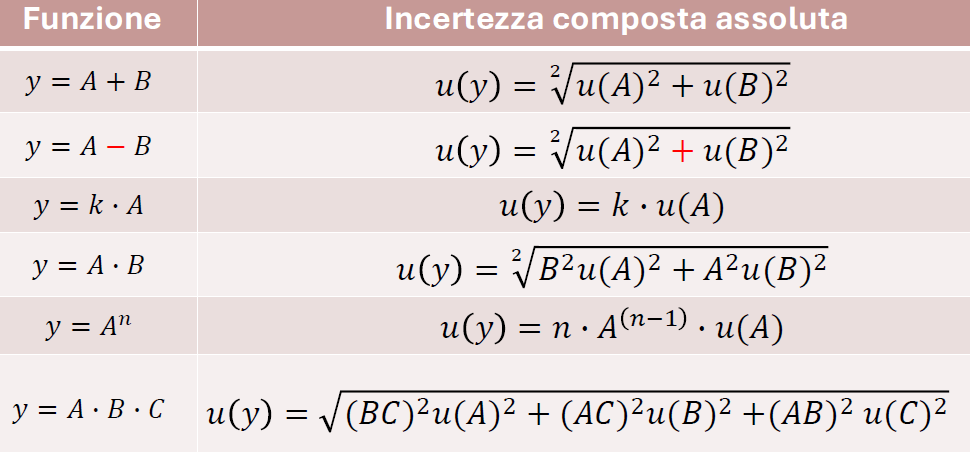
\includegraphics[scale = 0.3]{leggi di propagazione per legami funzionali semplici 2.PNG}
\end{figure}

\newpage

L'equazione per il calcolo di $u_c$ è spesso chiamata come legge di propagazione delle incertezze, 
ed è di grande utilità nella valutazione di incertezze per grandezze misurate per via indiretta. \newline 

La GUM consiglia, se possibile, di fare sempre misure dirette, ma, se ciò non è possibile, possiamo utilizzare queste relazioni. \newline 

Quando la funzione f non è definita e/o è difficile esplicitarla, si impiegano altri metodi alternativi, come ad esempio le simulazioni. \newline 

\newpage

\section{Supplemento GUM: simulazione Monte Carlo}
\footnote{Slide della prof | SDME 2 Incertezza secondo GUM parte II | pag 22 - 33 \\  
Appunti | 2025-03-05 | pag 9 - 10 | 2025-03-12 | pag 2 - 5}

\begin{tcolorbox}
    Questa sezione non la dobbiamo sapere bene e nel dettaglio come le altre: è un qualcosa in più
\end{tcolorbox}

Se la funzione tra le varie grandezze non è nota in maniera analitica e/o completa, il supplemento della GUM (il JCGM 101:2008) 
consiglia di implementare la simulazione Monte Carlo per il calcolo  delle propagazioni. \newline 

La simulazione Monte Carlo (in generale tutte le simulazioni perchè impiegano tempo e risorse) va utilizzata se: 

\begin{itemize}
    \item il modello funzionale devia fortemente dalla linearità 
    \item le derivate parziali sono difficilmente calcolabili 
    \item le distribuzioni di probabilità associate alle grandezze da misurare non sono gaussiane 
    \item la propagazione delle incertezze fornisce una sovrastima dell'incertezza associata alla misura finale 
    \item modello funzionale non completamente noto 
    \item modello funzionale complicato
\end{itemize}

Per la simulazione Monte Carlo si sceglie almeno un numero di $10^{6}$ simulazioni. \newline 

\newpage 

\section{Esprimere l'incertezza}
\footnote{Slide della prof | SDME 2 Incertezza secondo GUM parte II | pag 34 \\  
Appunti | 2025-03-12 | pag 5 - 6}

Possiamo riassumere tutto questo capitolo con i seguenti passaggi. \newline 

Di seguito, l'algoritmo step-by-step per esprimere l'incertezza di una misura: 

\begin{enumerate}
    \item Descrivere chiaramente il metodo usato per calcolare il risultato della misura e l'incertezza correlata 
    \item  Riportare una lista contenente tutte le componenti dell'incertezza e come esse sono state calcolate 
    \item Nel caso di incertezza estesa $U(x) = k \cdot u_c (x)$ occorre: 
    \begin{itemize}
        \item Fornire una descrizione esaustiva di come il parametro è definito 
        \item Riportare il risultato della misurazione come $X = x \pm U$ fornendo l'unità di misura 
        \item Fornire l'incertezza estesa relativa $U / \abs{x}$ 
        \item Riportare il valore di k 
        \item Fornire il livello di confidenza approssimato associato con l'intervallo $x \pm U$ e come è stato calcolato
    \end{itemize}
    \item Se si misurano due grandezze contemporaneamente, oltre alla misura e alle incertezze relative ad ogni parametro, bisogna fornire la covarianza ed il coefficiente di correlazione
\end{enumerate}

\begin{tcolorbox}
    L'ultimo punto riguardo la covarianza è vero in generale per tutte le misure, ma, come ho scritto precedentemente, in questo corso consideriamo grandezze indipendenti 
    in cui la covarianza è nulla. \newline 

    Si, in questo corso scriverò più e più volte le stesse cose, è un po' come andare a lezione: \\ 
    repetita iuvant , dicevano i romani
\end{tcolorbox}

\newpage 


\chapter{Incertezza strumentale e regole di scrittura}

\begin{figure}[h]
    \centering
    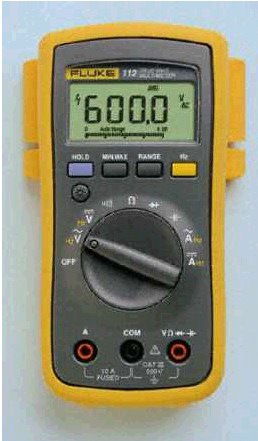
\includegraphics[scale = 1]{Fluke 112.png}
\end{figure}

\newpage 

\section{Il processo "reale" di misurazione}
\footnote{Slide della prof | SDME 2 Incertezza strumentale e regole di scrittura | pag 3 \\  
Appunti | 2025-03-12 | pag 6}

Di seguito la definizione di Misura data dalla norma UNI 4546: \newline

\textbf{Misura} : Informazione costituita da un valore, una incertezza ed una unità di misura, 
assegnata a presentare un parametro in un determinato stato del sistema. \newline 

Come si vede da un esempio di misura: 

\begin{figure}[h]
    \centering
    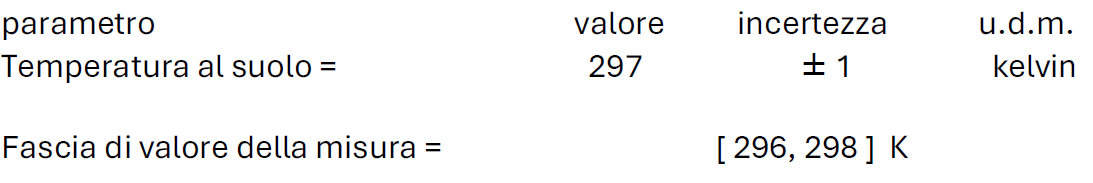
\includegraphics[scale = 0.5]{Esempio di misurazione.PNG}
\end{figure}

la misura è uno qualunque dei valori compresi nella fascia tra 297-1 kelvin e 297+1 kelvin. \newline 

\newpage 

\section{Incertezza degli strumenti di misura}
\footnote{Slide della prof | SDME 2 Incertezza strumentale e regole di scrittura | pag 4 \\  
Appunti | 2025-03-12 | pag 6 - 7}

Ciò che differisce il mondo ideale a quello reale è che 
gli strumenti di misura sono afflitti principalmente da tre effetti: 

\begin{itemize}
    \item Incertezza dei campioni negli strumenti 
    \item Deriva termica 
    \item Imprecisioni costruttive dello strumento 
\end{itemize}

Dalle specifiche degli strumenti, 
si ricava l'incertezza strumentale (in inglese accuracy). \newline 

Ad esempio, dalle specifiche del multimetro di questo multimetro Fluke 112: 

\begin{figure}[h]
    \centering
    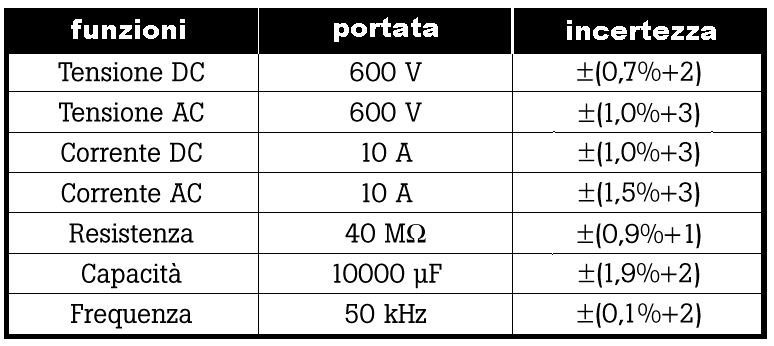
\includegraphics[scale = 0.5]{Specifiche Fluke 112.png}
\end{figure}

si nota nota che, nella colonna incertezza di questo strumento, l'incertezza è espressa in formula binomia. \newline 

Per formula binomia si intende una incertezza che è composta come: 

{
    \Large 
    \begin{equation}
        \pm (\text{ Percentuale del valore letto sul display} + \text{Numero digit})
    \end{equation}
}

La percentuale del valore letto sul display varia in base al valore che si legge sul display, 
invece il numero di digit è un contributo fisso. \newline 

Sempre dalla tabella delle specifiche tecniche del Fluke 112, possiamo notare che, 
per ogni tipologia di grandezza che lo strumento può misurare, il costruttore dichiara portata e accuracy con cui lo strumento opera. \newline 

\newpage 

\subsection{Incertezza dei campioni utilizzati}
\footnote{Slide della prof | SDME 2 Incertezza strumentale e regole di scrittura | pag 5 - 6 \\  
Appunti | 2025-03-12 | pag 7 - 8}

Gli strumenti utilizzano uno o più campioni di una grandezza all'interno del loro strumento per svolgere una misura. \newline 

Come riportato nel DataSheet dell'integrato AD587 dell'Analog Devices: 

\begin{figure}[h]
    \centering
    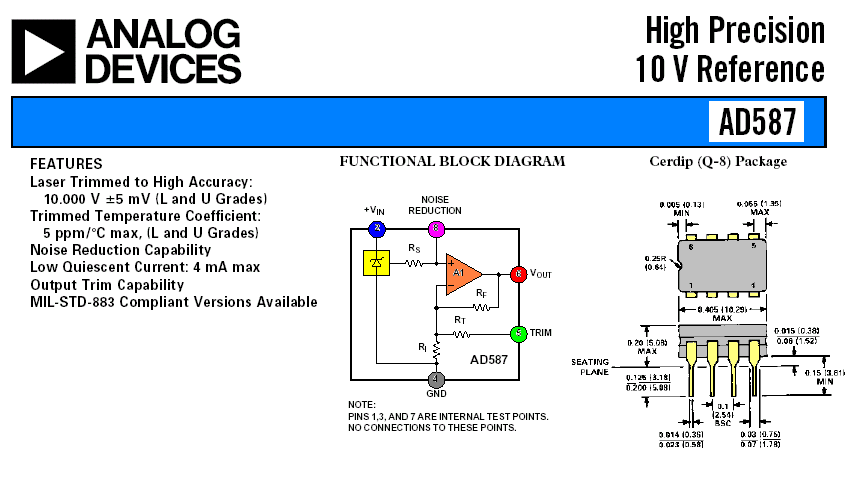
\includegraphics[scale = 0.5]{AD587 specs.png}
\end{figure}

l'integrato è un campione di riferimento di 10.000 V con incertezza di $\pm 5 \text{ } mV$. \newline 

Anche i campioni che materializzano le u.d.m. nei nostri strumenti sono affetti da incertezza (accuracy). \newline 

Tutte le misure che verranno fatte rapportando il valore della tensione incognita a questo valore campione saranno affette da alterazione ed essa sarà in parte proporzionale 
all'entità della tensione incognita stessa. \newline 

Si può corregge e minimizzare questa alterazione con la taratura. \newline 

O, in altri termini, l'incertezza proporzionale esiste perchè, generalmente, 
la misura viene fatta per confronto rispetto ad un riferimento, il quale ha a sua volta una sua incertezza. \newline 

\newpage 

\subsection{Deriva termica del campione}
\footnote{Slide della prof | SDME 2 Incertezza strumentale e regole di scrittura | pag 7 \\  
Appunti | 2025-03-12 | pag 8}

Come riportato nel DataSheet dell'integrato AD587 dell'Analog Devices, l'integrato di 10 V di riferimento è affetto da $5 \text{ } ppm/^{\circ} C $ max,
cioè il riferimento varierà massimo di 5 parti per milione per ogni grado centigrado. \newline 

A differenza dell'incertezza sul valore nominale, l'effetto della temperatura sul valore di tensione non può essere corretto con la taratura. \newline 

Si può eseguire la taratura per confronto con un campione di qualità superiore, a temperatura controllata, 
ma, a seguito della taratura, non si può garantire che la temperatura resti la stessa durante le operazioni di misura. \newline 

Basti banalmente capire la differenza e la stabilità della temperatura tra un laboratorio, dove la temperatura è controllata e stabile, 
e la temperatura "nel campo" di un tester. \newline 

\newpage 

\section{Imprecisioni costruttive dello strumento}
\footnote{Slide della prof | SDME 2 Incertezza strumentale e regole di scrittura | pag 8 - 9 \\  
Appunti | 2025-03-12 | pag 8}

Lo strumento è affetto anche esso dalla deriva termica, che, come sottolineato dalla deriva termica dei campioni, non si può modificare e/o 
calibrare con una taratura. \newline 

Ponendo ad esempio il tester Fluke 112, lo strumento contiene un campione di f.e.m. di 10 V, ma il costruttore dichiara una portata per le misure di tensione 
DC di 600 V. \newline

Ciò è possibile grazie a opportuni circuiti di confronto come, ad esempio, 
un partitore di tensione. \newline 

Come studiato dall'Elettrotecnica (mitico Stefano Squartini), 
un partitore di tensione è un circuito composto da due o più resistori in serie come in figura: 

\begin{figure}[h]
    \centering
    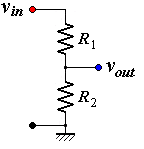
\includegraphics[scale = 1]{Partitore di tensione con due resistori.png}
\end{figure}

Sapendo i valori dei due resistori, cioè:

{
    \Large 
    \begin{equation} 
        \begin{cases}
            R_1 = R_{1 \text{nominale}} + \delta R_1
            \\ 
            R_2 = R_{2 \text{nominale}} + \delta R_2
        \end{cases}
    \end{equation}
}

dove $\delta R_1$ e $\delta R_2$ sono le tolleranze dei resistori reali rispetto ai valori nominali. \newline 

Sempre dall'Elettrotecnica, la tensione di uscita $v_{out} (t)$ sarà: 

{
    \Large 
    \begin{equation}
        v_{out} (t)
        = 
        \frac{R_2}{R_1 + R_2} v_{in} (t)
    \end{equation}
}

Essendo: 

{
    \Large 
    \begin{equation}
    \frac{R_2}{R_1 + R_2} < 1       
    \end{equation}
}

la tensione di ingresso $v_{in} (t)$ sarà diminuita: questo coefficiente prende il nome di rapporto di partizione 
e viene utilizzato dai costruttori di strumenti per confrontare la tensione di ingresso con la tensione di riferimento, i quali possono differire di diversi ordini di grandezza. \newline 

Aggiungendo anche le tolleranze dei due resistori, possiamo esprimere $v_{out} (t)$ come: 

{
    \Large 
    \begin{equation}
        v_{out} (t)
        = 
        \frac{R_{2 \text{nominale}} + \delta R_2}{ R_{1 \text{nominale}}+ R_{2 \text{nominale}} + \delta R_1 + \delta R_2} v_{in} (t) 
    \end{equation}
}

I valori di $\delta R_1$ e $\delta R_1$ sono presenti anche nell'espressione di $ v_{out} (t)$, 
quindi anche  $ v_{out} (t)$ varierà a causa della temperatura. \newline 

Sempre dall'espressione di  $ v_{out} (t)$, l'alterazione agisce in modo proporzionale. \newline 

Come scritto precedentemente, per ovviare alle imprecisioni costruttive dello strumento 
si possono tarare i campioni di riferimento delle grandezze, in genere il campione di f.e.m. . \newline 

La taratura e la certificazione dal LAT aggiungono un costo economico allo strumento di misura, 
come si vede da questo screenshot di un negozio online di strumenti di misura: 

\begin{figure}[h]
    \centering
    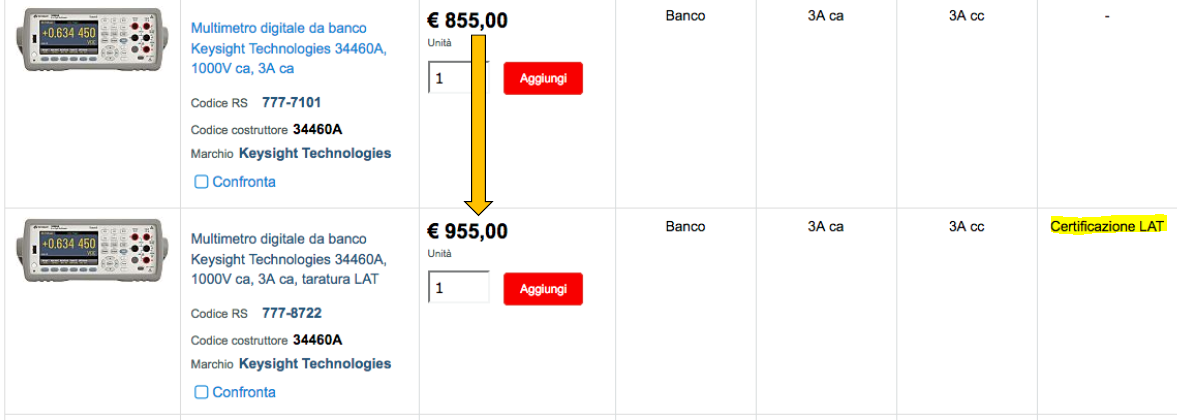
\includegraphics[scale = 0.5]{Confronto tra strumenti di misura con e senza certifiazione LAT.PNG}
\end{figure}


\newpage 

\subsection{Deriva termica dell'Offset degli OpAmp}
\footnote{Slide della prof | SDME 2 Incertezza strumentale e regole di scrittura | pag 10 \\  
Appunti | 2025-03-12 | pag 8}

All'interno degli strumenti di misura, sono inseriti gli amplificatori operazioni, 
strumenti non lineari inseriti per svolgere dei calcoli matematici (capirete meglio in futuro quando discuteremo delle architetture degli strumenti). \newline 

\begin{tcolorbox}

    Vi lascio dei video per rinfrescare la memoria su cosa sono gli amplificatori operazioni (detti e abbreviati in inglese OpAmp) dal corso di Elementi di Elettronica: 
    \begin{itemize}
        \item EEVblog \# 600 - OpAmps Tutorial - What is an Operational Amplifier?\\ \url{https://youtu.be/7FYHt5XviKc?si=4V3S8tFyC56y07hG} 
        \item What is an operational amplifier? - by Khan  Academy\\ \url{https://youtu.be/lJDjWZqhpVc?si=MouXEfN111w36XkM} 
    \end{itemize}

    Un fenomeno molto importante degli OpAmp è quello della massa virtuale (virtual ground in inglese), spiegati in questi video: 
    \begin{itemize}
        \item Virtual ground - by  by Khan  Academy\\ \url{https://youtu.be/pxKLeIjzxAk?si=qQZbF8nnEPm39s_I} 
        \item Guest Video: Bob DuHamel - How Opamp Virtual Grounds Work\\ \url{https://youtu.be/HbMnQdRzD8A?si=j4Np3j3G4TOOuCNx} 
    \end{itemize}

    L'ultimo video l'ho lasciato solo per il meme e perchè aveva una copertina alquanto bizzarra. \newline 
    Tutti i video sono disponibili con le traduzioni automatiche in Italiano di Youtube
\end{tcolorbox}

Il problema maggiore dei OpAmp nel mondo fisico reale (o come scrivono i Gen Z su internet, in IRL), è che sono affetti, anche loro, dalla deriva termica. \newline 

Le derive termiche, come scritto precedentemente, non possono essere corretti con la taratura. \newline 

Ad esempio dalla configurazione invertente di OpAmp come in figura: 

\begin{figure}[h]
    \centering
    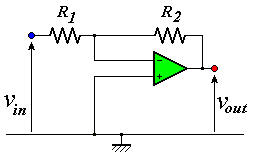
\includegraphics[scale = 1]{Configurazione invertente di un OpAmp.png}
\end{figure}

dove, si dimostra (cioè non lo dimostriamo) che la tensione $v_{out} (t)$ è: 

{
    \Large 
    \begin{equation}
        v_{out} (t) = - \frac{R_2}{R_1} v_{in} (t)
    \end{equation}
}

Nella realtà, dovremmo modellare il precedente in questa maniera: 

\begin{figure}[h]
    \centering
    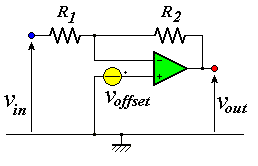
\includegraphics[scale = 1]{Configurazione invertente di un OpAmp reale.png}
\end{figure}

\newpage 

dove, rispetto al caso ideale, è presente una tensione di offset $V_{offset}$. \newline 

La tensione $V_{out}$ in uscita sarà: 

{
    \Large 
    \begin{equation}
        v_{out} (t) = - \frac{R_2}{R_1} 
        \left[ v_{in} (t) - v_{offset} (\theta) \right]
    \end{equation}
}

Nella realtà, le imperfezioni costruttive fanno nascere un contributo alla tensione di uscita dovuto alla temperatura (che abbiamo espresso nella funzione di $v_{out}$ con il simbolo $\theta$) 
che schematizzano con la nascita di una tensione di offset. \newline 

Per tensione di offset si intende che se $V_{in}$ è nulla, a $V_{out}$ sarà presente una tensione, che è uguale a $v_{offset}$. \newline 

\begin{tcolorbox}
    Se vuoi approfondire perchè si genera una tensione di offset all'ingresso di un OpAmp, ti lascio il seguente video: \newline 
    Offset voltage in op-amps (Amplifiers \# 8) - by Aaron Danner \\ \url{https://www.youtube.com/watch?v=biZ30H4bhks} \newline 

    In breve, la tensione di offset è dovuto alla rete circuitale dell'OpAmp
\end{tcolorbox}

\newpage 

\section{Perturbazione dello stato del sistema}
\footnote{Slide della prof | SDME 2 Incertezza strumentale e regole di scrittura | pag 11-12 \\  
Appunti | 2025-03-12 | pag 9 | 2025-04-14 | pag 2 - 3}

Nel caso ideale, se volessimo misurare la tensione ai capi di un generatore di tensione, 
lo schema circuitale sarebbe quello seguente: 

\begin{figure}[h]
    \centering
    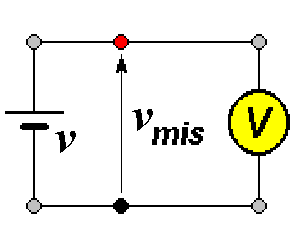
\includegraphics[scale = 0.6]{Tensione misurata caso ideale.png}
\end{figure}

Grazie all'elettrotecnica, nella realtà, una batteria stilo che "compriamo al supermercato" come quella in figura: 

\begin{figure}[h]
    \centering
    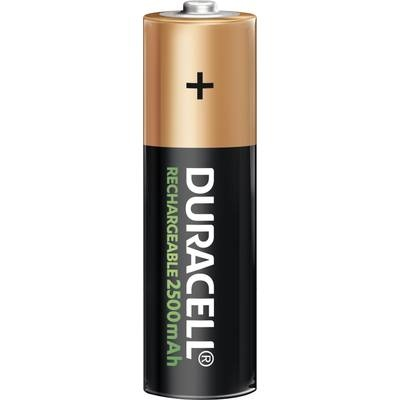
\includegraphics[scale = 0.2]{Batteria duracell.jpg}
\end{figure}

ha una sua rappresentazione che non sarà un generatore indipendente di tensione, 
bensì sarà un generatore indipendente di tensione con in serie una resistenza di Thevenin. \newline 

\begin{tcolorbox}
    Se serve un piccolo ripasso su cosa è la rappresentazione di Thevenin, 
    puoi vedere il seguente video: \newline 
    Elettrotecnica - Lezione 14 - Equivalente di Thevenin e Norton - di Elettronicamente\\ \url{https://youtu.be/cyw17JX1sd4?si=nsyMihd74wiDm8JG}
\end{tcolorbox}

Il nuovo circuito di misura sarà il seguente: 

\begin{figure}[h]
    \centering
    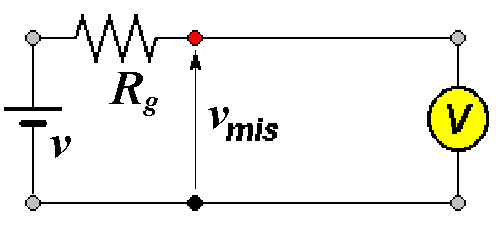
\includegraphics[scale = 0.6]{Circuito di misura con rappresentazione di Thevenin.png}
\end{figure}

Quindi, se la tensione misurata non sarà la tensione ai capi del generatore di tensione, bensì: 

{
    \Large 
    \begin{equation}
        \begin{cases}
            v_{mis} = v - v_{R_{g}} 
            \\ 
            v_{mis} \neq v
        \end{cases}
    \end{equation}
}

dove $v_{R_{g}}$ è la tensione ai capi del resistore $R_g$. \newline 

Per riassumere, la tensione che andremo realmente a misurare non sarà quella a vuoto del generatore, 
ma quella "sotto carico" ovvero la $v_{mis}$. \newline 

Per modellare un voltmetro reale, si pone la sua resistenza $R_v$ in parallelo ad esso.\newline 

Il nuovo circuito di misura sarà il seguente: 

\begin{figure}[h]
    \centering
    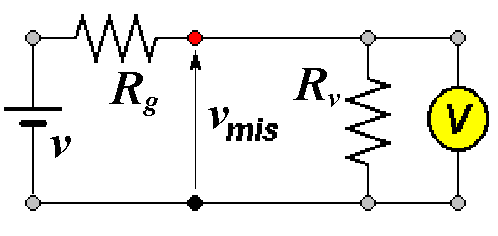
\includegraphics[scale = 0.6]{Circuito di misura con rappresentazione di Thevenin e Norton.png}
\end{figure}

In un voltmetro ideale, lo strumento è caratterizzato da impedenza di ingresso $R_v$ infinita 
che non viene attraversata da nessuna corrente. \newline 

In un voltmetro reale, lo strumento ha una sua impedenza $R_v$ in cui scorre corrente: 
lo strumento diventa un partitore di tensione. \newline 

La tensione che realmente misureremo sarà: 

{
    \Large 
    \begin{equation}
        \begin{cases}
            v_{mis}
            = 
            v \frac{R_v}{R_g + R_v} 
            \\ 
            v_{mis}
            \neq 
            v
        \end{cases}
    \end{equation}
}

A causa di questa $R_v$ del voltmetro reale, avviene una perturbazione del sistema. \newline 

Possiamo calcolare $\delta v$, cioè la differenza tra la tensione misurata e quella ideale, come: 

{
    \Large 
    \begin{equation}
        \begin{split}
            \delta v
            &= 
            v_{mis} - v 
            \\ 
            &= 
            v \frac{R_v}{R_g + R_v} - v 
            \\
            &= 
            - \frac{R_v}{R_g + R_v} v
        \end{split}
    \end{equation}
}

$\delta v$ è di segno negativo, quindi si sottostimerà la tensione $v_{mis}$. \newline 

Se svolgiamo il rapporto tra $\delta v$ e v abbiamo: 

{
    \Large 
    \begin{equation}
        \frac{\delta v}{v}
        = 
        - \frac{R_v}{R_g + R_v}
    \end{equation}
}

Se $R_v >>> R_g$, cioè $R_v$ è molto più grande rispetto a $R_g$, 
il denominatore di $\frac{\delta v}{v}$ tenderà a zero e/o diminuirà di molto. \newline 

\newpage 

\section{Disturbi e rumori elettrici, magnetici ed elettromagnetici}
\footnote{Slide della prof | SDME 2 Incertezza strumentale e regole di scrittura | pag 13 \\  
Appunti | 2025-03-14 | pag 3}

Nel mondo fisico e reale in cui viviamo, possono verificarsi dei disturbi elettromagnetici non voluti. \newline 

In base alla frequenza che vogliamo misurare, possiamo utilizzare questo grafico per rappresentare 
quanto il disturbo elettromagnetico impatta la misura: 

\begin{figure}[h]
    \centering
    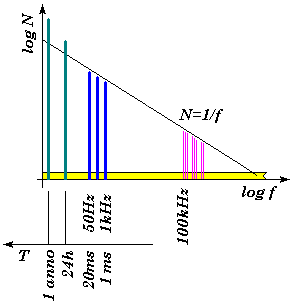
\includegraphics[scale = 0.8]{Disturbi elettromagnetici in base alla frequenza.png}
\end{figure}

I disturbi elettromagnetici sono causati da dispositivi non lineari. \newline 

Generalmente, i dispositivi di misura sono protetti da questi disturbi, ma è sempre meglio a priori accorgersi 
e prendere degli accorgimenti riguardo i disturbi elettromagnetici presenti nell'ambiente in cui si vuole fare la misura, 
perchè, oltre alla grandezza che si vuole misurare, misureremo anche il disturbo stesso, che si sommerà alla grandezza da misurare. \newline 

Inoltre, i disturbi sono difficili da identificare. \newline 

Ritornando alla figura dei disturbi di rete e delle armoniche generate dai dispositivi non lineari (cioè la figura sovrastante), 
se si vuole misurare una grandezza per 1 anno o 24 ore, la misura sarà afflitta da disturbi dovute alla derive termiche. \newline 

I disturbi a 50 Hz e 1 kHz sono dovuti alla rete elettrica, in particolare agli interruttori switching presenti nei dispositivi che abbiamo in casa. \newline 

Invece, i disturbi ad alta frequenza, cioè oltre i 100 kHz, sono dovuti alle radiocomunicazioni e al rumore termico. \newline 

La riga gialla indica il rumore termico che è AWGN (Additive White Gaussian Noise), cioè a spettro piatto e presente in tutte le frequenze. \newline 

\newpage 

\section{Incertezza strumentale: bit e digit}
\footnote{Slide della prof | SDME 2 Incertezza strumentale e regole di scrittura | pag 14 \\  
Appunti | 2025-03-14 | pag 4}

Visto che oramai ogni giorno abbiamo a che fare con uno strumento di misura digitale, 
lo strumento ci mostra, generalmente sul suo display, diverse cifre. \newline 

Siccome questi strumenti digitali contengono dei registri, ogni numero sarà 
rappresentato e interpretato dalla circuiteria come una serie di valori binari. \newline 

Per esempio il numero in decimale 149, in binario diventa: 
{
    \Large
    \begin{equation}
        149_{10} 
        \to 
        1001\text { } 0101_{2}
    \end{equation}
}

Si può fare anche il processo inverso, partendo dalla cifra più a sinistra e andando verso destra: 

{
    \Large 
    \begin{equation}
        \begin{split}
        1001\text { } 0101 
        &= 
        2^{7} + 2^{4} + 2^{2} + 2^{0} 
        \\ 
        &= 
        128 + 16 + 4 + 1 
        \\ 
        &= 
        149
        \end{split}
    \end{equation}
}

\begin{tcolorbox}
    Se vuoi ripassare un po' le conversioni tra le basi numeriche: \newline 
    \url{https://www.youmath.it/domande-a-risposte/view/8207-da-decimale-a-binario.html}
\end{tcolorbox}

Quindi, il primo bit, quello più a destra viene nominato come LSB (Least Significant Bit), 
invece l'ultimo bit, quello più a sinistra, viene definito come MSB (Most Significant Bit). \newline 

Prendono questo nome, proprio perchè, come visto dalla conversione del numero digitale a quello decimale, 
i bit più a sinistra hanno un peso maggiore rispetto quelli a destra. \newline 

In questo caso $2^{7} > 2^{0}$. \newline 

Lo stesso principio dei pesi dei bit in base al loro ordine, lo si può applicare alle cifre che ci vengono fornite dallo strumento di misura. \newline 

In questo caso non si descriveranno i bit bensì i digit. \newline 

In figura un esempio di valori in un voltmetro e del suo display: 

\begin{figure}[h]
    \centering
    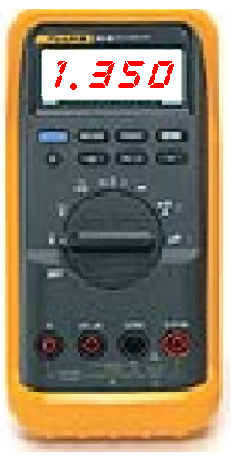
\includegraphics[scale = 0.6]{Digits in un voltmetro.PNG}
\end{figure}

\newpage 

La cifra 0 che si trova a destra viene definita LSD (Least Significant Digit), 
invece la cifra 1 che si trova a sinistra viene definita come MSD (Most Significant Digit). \newline 

\newpage 

\subsection{Espressione della incertezza degli strumenti indicatori (accuracy) - il "digit"}
\footnote{Slide della prof | SDME 2 Incertezza strumentale e regole di scrittura | pag 15 \\  
Appunti | 2025-03-14 | pag 4 - 5}

Se, ad esempio, abbiamo nel display del nostro strumento le cifre: 

{
    \Large 
    \begin{equation}
        1.350 \text{ [V]}
    \end{equation}
}

La formula simbolica per il calcolo dell'accuracy è la seguente: 

{
    \Large 
    \begin{equation}
        \Delta g \text{ } = \pm (a \% \text{ lettura }+ b \text{ digit }) 
    \end{equation}
}

Se dal produttore del voltmetro abbiamo la seguente indicazione del calcolo dell'accuracy: 

{
    \Large 
    \begin{equation}
        \Delta g \text{ } = \pm (1 \% \text{ lettura }+ 2 \text{ digit }) 
    \end{equation}
}

Generalmente la GUM consiglia 1 o 2 digit per il calcolo dell'accuracy. \newline 


Calcoliamo la prima parte dell'accuracy: 

{
    \Large 
    \begin{equation}
        \begin{split}
            \Delta g_{\text{lettura}}
            &= 
            1.350 \text{ [V]} 
            \cdot 1 \% 
            \\ 
            &= 
            0.0135 \text{ [V]}
        \end{split}
    \end{equation}
}

Considerando 2 digit, significa che da $\Delta g_{\text{lettura}}$ si considerano, 
partendo da sinistra andando verso destra, 2 cifre diverse da zero. \newline 

Quindi, $\Delta g_{\text{lettura}}$ diventa: 

{
    \Large 
    \begin{equation}
        \Delta g_{\text{lettura}} = 0.013
    \end{equation}
}

oppure, per notazione, si può anche scrivere le cifre che non comprendono i digit in minuscolo. \newline 

In questo particolare caso è valida anche la seguente notazione: 

{
    \Large 
    \begin{equation}
        \Delta g_{\text{lettura}} = 0.013_{5}
    \end{equation}
}

perchè il valore 5 è quel valore intermedio nell'intervallo. \newline 

Il valore 5 generalmente si arrotonda per eccesso, ma, scritto in questa maniera, si lascia all'utente finale se svolgere l'arrotondamento per eccesso o meno. \newline 

Siccome si considerano 2 digit, il secondo digit diverso da zero esprime 1 [mV], quindi: 

{
    \Large 
    \begin{equation}
        \begin{split}
            \Delta g_{\text{digit}} 
            &= 
            2 \cdot 1 \text{ [mV]}
            \\ 
            &= 
            2 \text{ [mV]}
        \end{split}
    \end{equation}
}

Combinando i due fattori $\Delta g_{\text{lettura}}$ e $\Delta g_{\text{digit}} $, 
si può esprimere $\Delta g$ come: 

{
    \Large 
    \begin{equation}
        \begin{split}
            \Delta g 
            &= 
            \pm 
            (\Delta g_{\text{lettura}} + \Delta g_{\text{digit}} ) \text{ [V]} 
            \\
            &=
            \pm 
            (0.0135_{5} + 0.002) \text{ [V]}
        \end{split}
    \end{equation}
}

Questo è un caso particolare perchè l'ultimo digit di $\Delta g_{\text{lettura}}$ è uguale a 5, 
quindi si va alla cifra superiore: 

{
    \Large 
    \begin{equation}
        \begin{split}
            &= 
            \pm 
            0.01_{55} \text{ [V]}
            \\ 
            &= 
            \pm 
            0.02 \text{ [V]}
        \end{split}
    \end{equation}
}

$\Delta g \text{ }= \text{ } \pm 0.02 \text{ [V]} $ è il valore di a, 
dalla quale si calcola l'incertezza di tipo B ipotizzando una pdf (densità di probabilità) dello strumento stesso. \newline 

\newpage 

\section{Riduzione della incertezza strumentale}
\footnote{Slide della prof | SDME 2 Incertezza strumentale e regole di scrittura | pag 16 \\  
Appunti | 2025-03-14 | pag 6}

Dalla definizione di misura della GUM, la misura è un processo, quindi anche la riduzione dell'incertezza è un processo. \newline 

Per ridurre l'incertezza, si possono applicare le seguenti accortezze: 

\begin{itemize}
    \item Periodicamente effettuare o richiedere la taratura dello strumento 
    \item Non eseguire misurazioni durante la fase di riscaldamento dello strumento, cioè non prima che sia superato il transitorio, perchè lo strumento è stato tarato ad una temperatura di riferimento che è quella di regime 
    \item Se si conoscono i parametri del sistema, si può calcolare la perturbazione dello stato del sistema provocata dallo strumento
\end{itemize}


Per quanto riguarda l'ultima accortezza, 
da un punto di vista analitico, 
dobbiamo determinare l'incertezza strumentale (cioè l'accuracy), 
se si ipotizza la pdf, per trovare la $u_{B} (x)$, 
che andrà combinata con la $u_{A} (x)$ e moltiplicata per un opportuno fattore di copertura k, per trovare U(x). \newline 

\newpage 

\section{Espressione della incertezza di misura}
\footnote{Slide della prof | SDME 2 Incertezza strumentale e regole di scrittura | pag 17 \\  
Appunti | 2025-03-14 | pag 6}

L'accuracy $\Delta g$ non solo può essere espressa nella formula scritta precedentemente, ma anche in altri modi. \newline 

Di seguito alcuni esempi. \newline 

\textbf{Incertezza assoluta} 

L'incertezza assoluta è l'ampiezza dell'intervallo centrato sul valore indicato x. \newline 

Si esprimere come: 

{
    \Large 
    \begin{equation}
        \Delta x = \pm \text{ } U
    \end{equation}
}


L'incertezza assoluta è dotata di dimensioni omogenee (cioè le stesse) alla grandezza sotto misura. \newline 

\textbf{Incertezza relativa} 

L'incertezza relativa è il rapporto fra i valori dell'incertezza assoluta $\Delta x$ e il valore indicato x. \newline 

Si esprime come: 

{
    \Large 
    \begin{equation}
        \frac{\Delta x}{x} 
        = 
        \pm 
        \frac{U}{x}
    \end{equation}
}

L'incertezza relativa, rispetto all'incertezza assoluta, è adimensionale. \newline 

Da un punto di vista qualitativo, aiuta a capire se la misura è di buona qualità. \newline 

\textbf{Incertezza percentuale}

L'incertezza percentuale esprime il valore dell'incertezza relativa moltiplicato per 100. \newline 

Si esprime come: 

{
    \Large 
    \begin{equation}
        \Delta x \% = \pm 100 \cdot \left(\frac{U}{x}\right)
    \end{equation}
}

Utilizzata comunemente nei contesti di misura. \newline 

\textbf{Incertezza relativa in ppm}

L'incertezza relativa in ppm (cioè parti per milione) esprime il valore dell'incertezza relativa moltiplicata per 1 000 000. \newline 

Si esprime come: 

{
    \Large 
    \begin{equation}
        \frac{\Delta x}{x} (ppm) 
        = 
        \pm 1 \cdot 10^{6} \cdot \left(\frac{U}{x}\right)
    \end{equation}
}

\newpage 

\section{Regola di scrittura: cifre significative}
\footnote{Slide della prof | SDME 2 Incertezza strumentale e regole di scrittura | pag 18 -21 \\  
Appunti | 2025-03-14 | pag 6 - 9}

Poniamo come esempio i seguenti dati: 

{
    \Large 
    \begin{equation}
        \begin{cases}
            x = 123.456 89 \text{ [V]} 
            \\ 
            U = \pm 0.001 41 \text{ [V]}
        \end{cases}
    \end{equation}
}

dove, come scritto precedentemente, U è l'incertezza assoluta e x è il valore letto sul display dello strumento. \newline 

Quindi x appartiene al seguente intervallo: 

{
    \Large 
    \begin{equation}
        \begin{split}
            123.456 89 - 0.001 41 \text{ [V] }
            < 
            \text{ }
            &x 
            \text{ }
            < 
            123.456 89 + 0.001 41 \text{ [V] }
            \\
            123.455 48 \text{ [V] }
            < 
            \text{ }
            &x 
            \text{ }
            < 
            123.458 30 \text{ [V] }
        \end{split}
    \end{equation}
}

Da un punto di vista grafico: 

\begin{figure}[h]
    \centering
    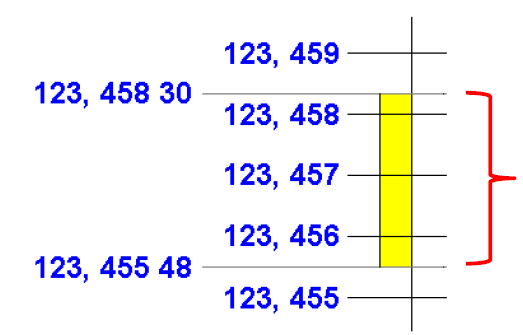
\includegraphics[scale = 0.5]{Intervallo di misura.PNG}
\end{figure}

Quella tratteggiata in rosso è la fascia dei valori della misurazione. \newline 

Ponendo la regola che ci dice la GUM, cioè esprimere l'incertezza 
con una o al massimo due cifre diverse da zero, e approssimando per eccesso, 
l'incertezza U diventa: 

{
    \Large 
    \begin{equation}
        \begin{split}
             U &= \pm 0.001 41 \text{ [V]}
             \\
             &\downarrow
             \\
             U &= \pm 0.002 \text{ [V]}
        \end{split}
    \end{equation}
}

Da un punto di vista grafico, non andremo a considerare l'intervallo precedente in giallo di prima, 
bensì quello verde che è più esteso:

\begin{figure}[h]
    \centering
    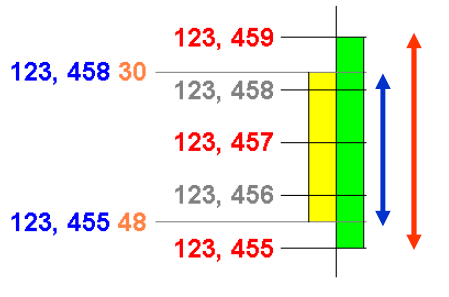
\includegraphics[scale = 0.5]{Intervallo di misura con approssimazioni.PNG}
\end{figure}


Inoltre, siccome abbiamo espresso l'incertezza, bisogna esprimere il valore centrale della misura. \newline 

Il valore centrale della misura diventa, 
applicando anche le approssimazioni e troncando alla stessa cifra dell'incertezza: 

{
    \Large 
    \begin{equation}
        \begin{split}
            x &= 123.456 89 \text{ [V]}
            \\ 
            &\downarrow 
            \\ 
            x &= 123.457 \text{ [V]}
        \end{split}  
    \end{equation}
}

Unendo il valore centrale e l'incertezza della misura insieme, 
la misura finale si può esprimere come: 

{
    \Large 
    \begin{equation}
        x = (123.457 \text{ } \pm \text{ } 0.002) \text{ [V]}
    \end{equation}
}

La regola aurea nelle misure è meglio esprimere una maggiore incertezza che una minore, 
e le incertezze vanno approssimate per eccesso, 
invece il valore medio al valore vicino. \newline 


\newpage 

\section{Compatibilità tra le misure}
\footnote{Slide della prof | SDME 2 Incertezza strumentale e regole di scrittura | pag 22 - 23 \\  
Appunti | 2025-03-14 | pag 9 - 10}

Un concetto molto importante dettate dalla GUM è quello di compatibilità. \newline

Essendo la misura un processo, due o più misure non possono essere uguali. \newline 

Al posto del concetto di uguaglianza, si sostituirà il concetto di compatibilità. \newline 

Diciamo che due misure di uno stesso misurando sono tra loro compatibili se gli intervalli dei valori "plausibili", 
ossia probabili ad un certo livello di confidenza che possono essere loro assegnati, 
hanno una adeguata sovrapposizione. \newline 

Da un punto di vista grafico: 

\begin{figure}[h]
    \centering
    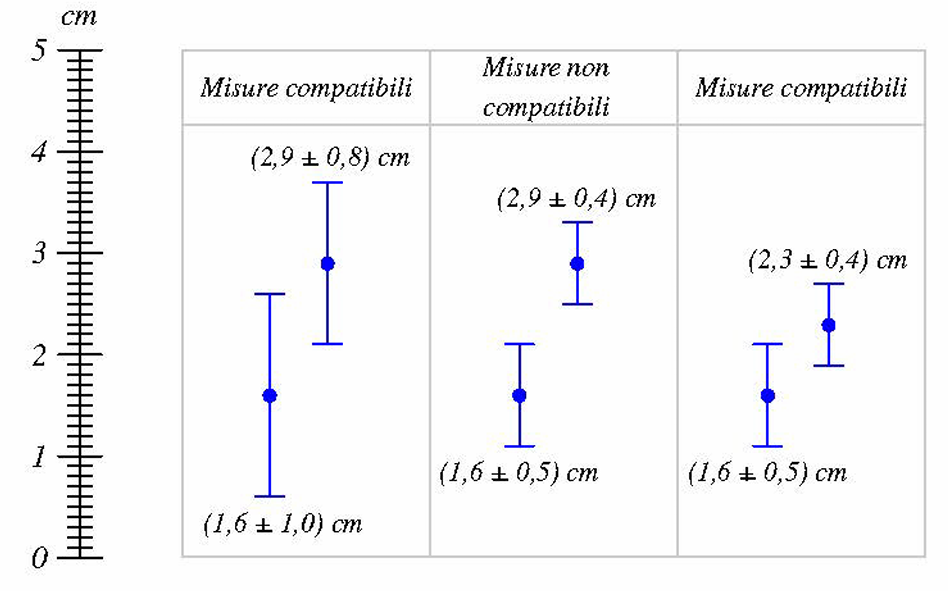
\includegraphics[scale = 0.3]{Esempio di misure compatibili.PNG}
\end{figure}

Per la definizione degli intervalli di compatibilità, 
è opportuno usare un adeguato fattore di ricopertura. \newline 

Il fattore di ricopertura lo indichiamo con la lettera a e deve essere: 

{
    \Large 
    \begin{equation}
        a \ge 1
    \end{equation}
}

a deve essere un numero intero. \newline

Nel caso di misure indipendenti, cioè non correlate, (quelle che studieremo in questo corso), 
la compatibilità si esprime come: 

{
    \Large 
    \begin{equation}
        \abs{x_1 - x_2} 
        \le 
        a \sqrt{u^{2}(x_1) + u^{2}(x_2)}
    \end{equation}
}

dove $x_1$ e $x_2$ sono i valori con le corrispettive incertezze $u(x_1)$ e $u(x_2)$. \newline 

Da un punto di vista pratico, 
normalmente si accetta la compatibilità se a ha un valore intero compreso tra: 

{
    \Large 
    \begin{equation}
        1 \leq a \leq 3
    \end{equation}
}


\newpage 

\subsection{Compatibilità tra le misure e media pesata}
\footnote{Slide della prof | SDME 2 Incertezza strumentale e regole di scrittura | pag 24 \\  
Appunti | 2025-03-14 | pag 10}

In presenza di un certo numero L di misure $x_1$, $x_2$, ..., $x_l$, ....., $x_L$ tra loro compatibili, 
il valore che si usa per esprimere il misurando è dato da una media pesata $\overline{x_{MP}}$ come: 

{
    \Large 
    \begin{equation}
        \begin{split}
            \overline{x_{MP}} 
            &= 
            \frac{\sum_{l=1}^{L} \frac{x_l}{u^{2} (x_l)}}
            {\sum_{l=1}^{L} \frac{1}{u^{2} (x_l)}}
            \\
            &= 
            \frac{\sum_{l=1}^{L} w_l x_l}
            {\sum_{l=1}^{L} w_l}
        \end{split}
    \end{equation}
}

dove: 

{
    \Large
    \begin{equation}
        w_l = \frac{1}{u^{2} (x_l)}
    \end{equation}
}

Dalla media pesata, si può calcolare il quadrato dell'incertezza stimata è data da: 

{
    \Large 
    \begin{equation}
        \begin{split}
            u^{2} (\overline{x_{MP}})
            &= 
            \frac{1}{\sum_{l = 1}^{L} \frac{1}{u^{2} (x_l)}}
            \\ 
            &= 
            \frac{1}{\sum_{l=1}^{L} w_l}
        \end{split} 
    \end{equation}
}


\chapter{Conversione AD e convertitori - parte I}

\begin{figure}[h]
    \centering
    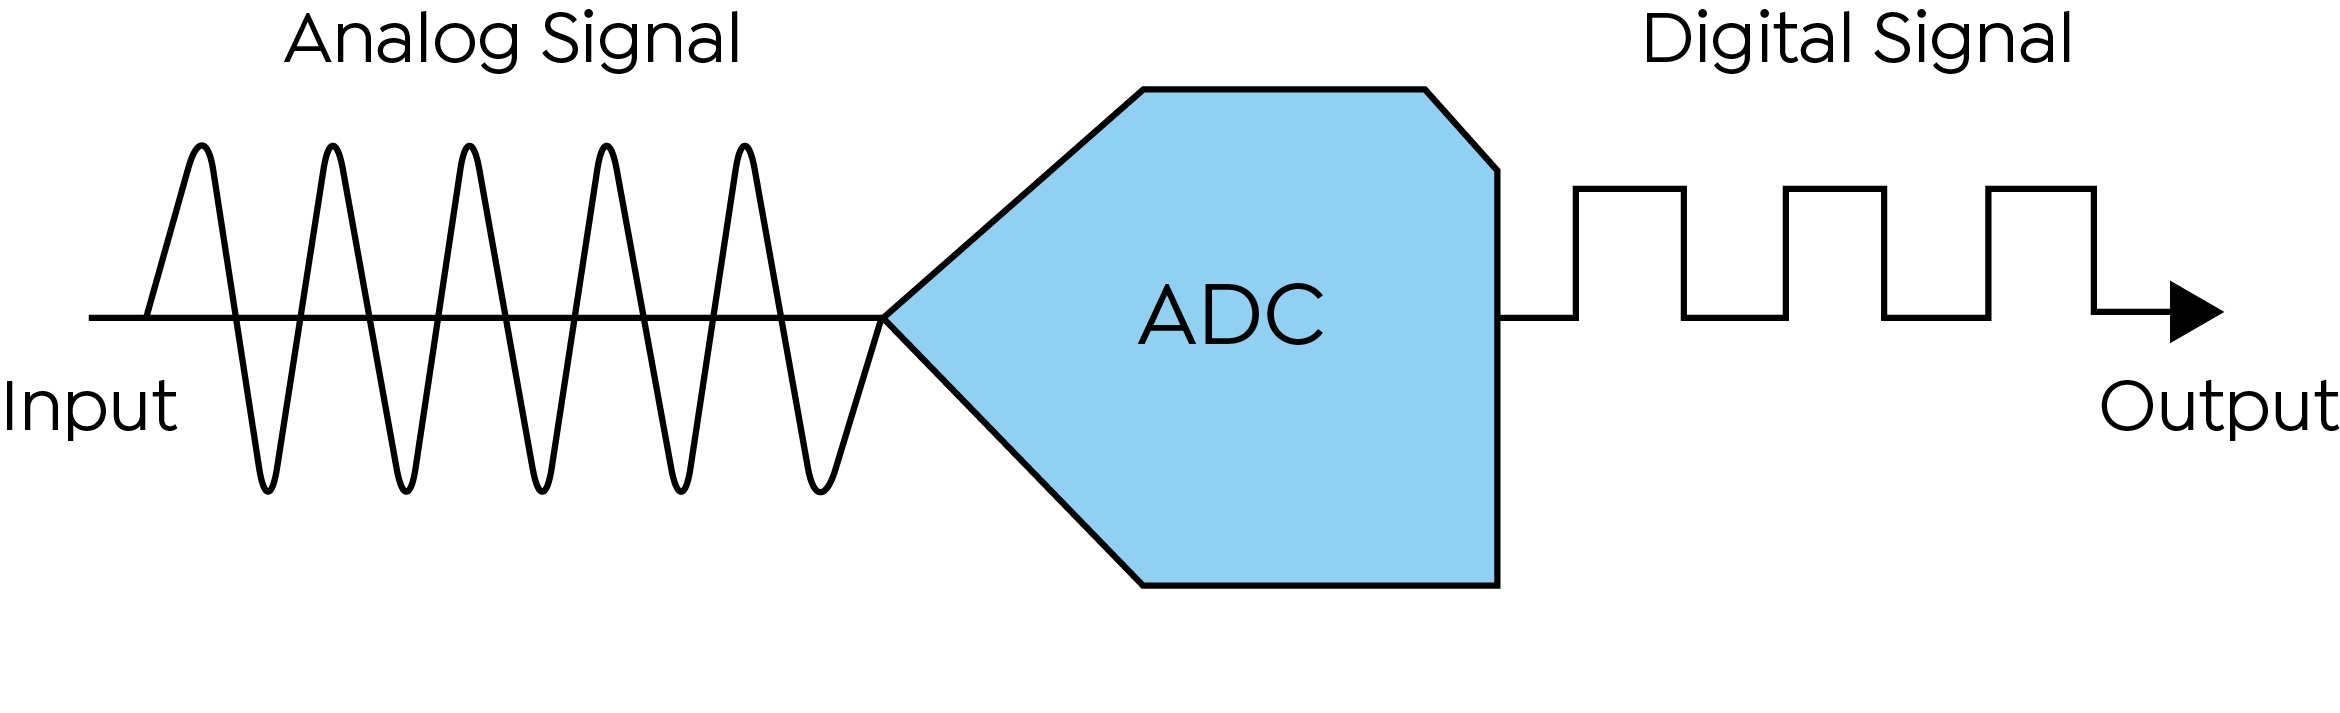
\includegraphics[scale = 0.3]{EBV_ST-Analog_Blockdiagramm_EBVA022-Figure3.jpg}
\end{figure}

\newpage 

\begin{tcolorbox}
    I concetti dei capitoli riguardo la conversione AD e dei vari convertitori sono già stati approfonditi in precedenti materie di questo corso di laurea. \newline 
    Adesso verranno approfonditi in ambito misuristico    
\end{tcolorbox}

\section{Segnali analogici e digitali}
\footnote{Slide della prof | SDME 3.Conversione AD e Convertitori - Parte I | pag 3 - 4 \\  
Appunti | 2025-03-18 | pag 2 - 3}

Si definisce segnale analogico un segnale che può essere rappresentato mediante una funzione del tempo che gode di due proprietà: 

\begin{itemize}
    \item la funzione è definita per ogni valore del tempo 
    \item la funzione è continua
\end{itemize}

Grazie a queste due proprietà, un segnale analogico ha infiniti valori. \newline 

Un esempio di segnale analogico: 

\begin{figure}[h]
    \centering
    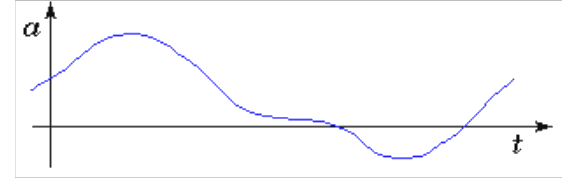
\includegraphics[scale = 0.4]{Esempio segnale analogico.png}
\end{figure}

Da un punto di notazione matematica, possiamo definire un segnale analogico come: 

{
    \Large 
    \begin{equation}
        \begin{cases}
            a = f(t) 
            \\ 
            t \in \mathbb{R}
            \\ 
            a \in \mathbb{R}
        \end{cases}
    \end{equation}
} 

Dagli infiniti valori dei casi continui, passiamo ai finiti valori 
(discreti valori) dei segnali digitali. \newline 

Un segnale digitale è rappresentato da una funzione a tempo discreto e quantizzata. \newline 

Ciò significa che: 

\begin{itemize}
    \item la funzione è definita solamente in un insieme numerabile di istanti, tipicamente equi-spaziata 
    \item la funzione è dotata di codominio costituito da un insieme discreto e numerabile di valori
\end{itemize}

La quantizzazione potrebbe avvenire con "quanti" di ampiezza diversa. \newline 

Un esempio di segnale digitale: 

\begin{figure}[h]
    \centering
    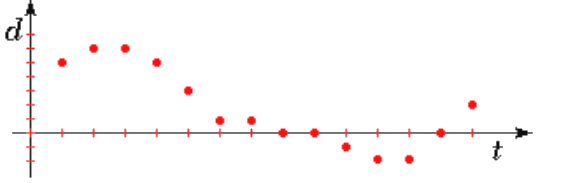
\includegraphics[scale = 0.4]{Esempio di segnale digitale.png}
\end{figure}

La funzione passa da un livello "consentito" ad un altro senza poter attraversare tutti i valori intermedi, 
quindi, da un punto di vista grafico, la funzione non è definita tra due punti. \newline 

La distanza tra due punti, nell'asse delle ascisse del tempo t, viene definito come periodo di campionamento $T_c$. \newline 

Da un punto di notazione matematica, possiamo definire un segnale digitale come: 

{
    \Large 
    \begin{equation}
        \begin{cases}
        d = f[n T_c]
        \\
        n \in \mathbb{Z}  
        \\ 
        d \in \mathbb{Z}
        \end{cases}
    \end{equation}
}

\begin{tcolorbox}
    Per distinguere tra segnale analogico e discreto, 
    come nel corso di DSP di Stefano Squartini, userò la notazione tra parentesi tonde () per indicare un segnale analogico, 
    mentre a parentesi quadre [ ] per un segnale discreto 
\end{tcolorbox}


\newpage 

\section{Interesse alle misure elettroniche}
\footnote{Slide della prof | SDME 3.Conversione AD e Convertitori - Parte I | pag 5 \\  
Appunti | 2025-03-18 | pag 3}

Tra tutte le tipologie di segnali, c'è interesse rispetto ai segnali elettrici analogici perchè presentano le seguenti proprietà: 

\begin{itemize}
    \item amplificabilità diretta 
    \item trasmissibilità a distanza 
    \item registrabilità 
    \item elaborabilità (come scritto precedentemente, si utilizzano gli OpAmp per svolgere i calcoli matematici)
\end{itemize}

Dai segnali analogici a quelli digitali, la misura diventerà una sequenza di numeri. \newline 

I segnali elettrici numerici, o digitali, esaltano ulteriormente queste proprietà: 

\begin{itemize}
    \item trasmissibilità a distanza (beneficia della natura discreta della f nel tempo) 
    \item registrabilità (segnali numerici consentono una maggiore densità di registrazione)
    \item elaborabilità (mediante algoritmi eseguiti da microprocessori o DSP)
    \item reiezione ai disturbi (un segnale digitale non risiede di disturbi fino ad una certa entità)
\end{itemize}

La possibilità di impiegare algoritmi eseguiti da microprocessori o DSP permette di elaborare il segnale con nuove versioni del 
software senza costruire fisicamente un nuovo circuito. \newline 

\newpage 

\subsection{Analogico vs Digitale: occupazione della linea}
\footnote{Slide della prof | SDME 3.Conversione AD e Convertitori - Parte I | pag 6 - 7 \\  
Appunti | 2025-03-18 | pag 3}


Dal punto di vista dell'occupazione della linea, il segnale analogico occupa permanentemente la linea di trasmissione, 
mentre quello digitale ne permette la condivisione con altri segnali. \newline 

Considerando due segnali analogici di un cavo jack stereo: 

\begin{figure}[h]
    \centering
    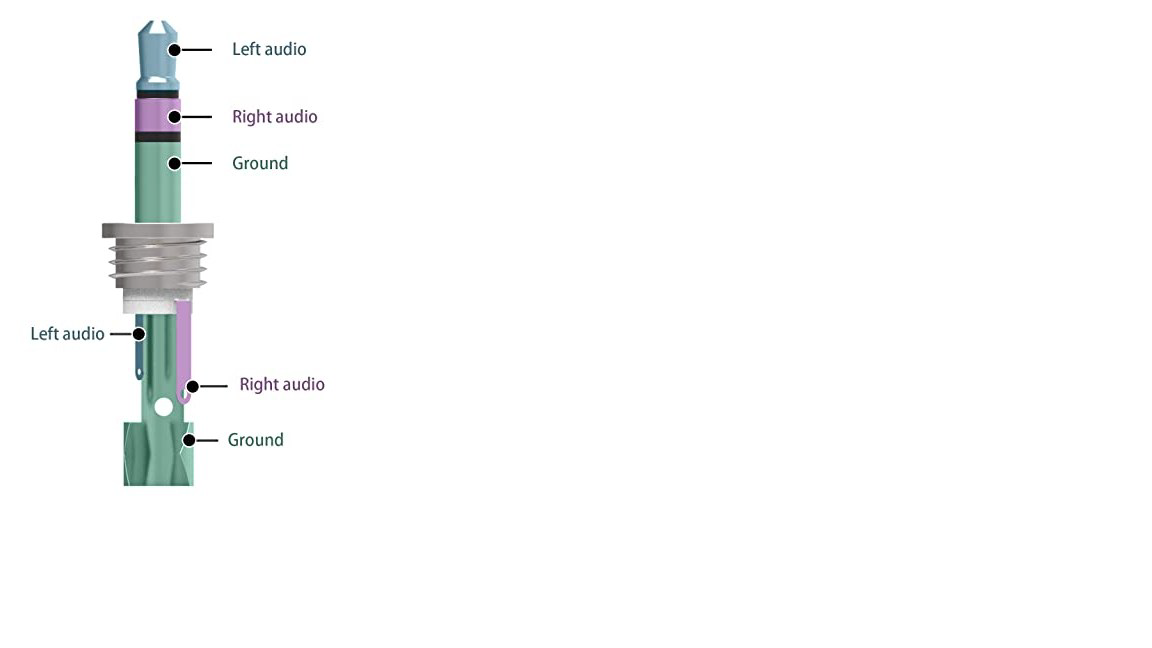
\includegraphics[scale = 0.4]{cavo jack stereo.png}
\end{figure}

Essendo un segnale definito in ogni istante, 
ogni segnale analogico necessita della linea in ogni singolo istante di tempo in cui esso esiste.\newline 

Quindi per trasmettere due segnali analogici, come in figura: 

\begin{figure}[h]
    \centering
    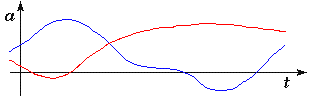
\includegraphics[scale = 1]{Due segnali analogici.png}
\end{figure}

occorrono 3 linee, due per i segnali e una per la massa come in figura: 

\begin{figure}[h]
    \centering
    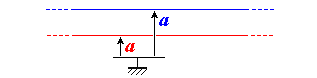
\includegraphics[scale = 1]{Due linee e massa in comune.png}
\end{figure}

Il segnale digitale necessita della linea solo nei singoli istanti di tempo in cui esso esiste ed è definito come si vede in figura: 

\begin{figure}[h]
    \centering
    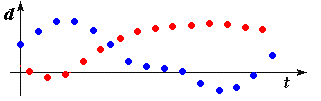
\includegraphics[scale = 0.8]{Due segnali digitali .png}
\end{figure}

\newpage 

Negli altri istanti, si può lasciare la linea libera e consentire la trasmissione di altri segnali digitali, come in figura: 

\begin{figure}[h]
    \centering
    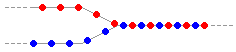
\includegraphics[scale = 0.8]{Condivisione nella stessa linea.png}
\end{figure}


Per inviare più segnali nella stessa linea, 
si possono multipare i segnali o in altri canali o in frequenza, 
e poi demultiplarli in ricezione, come si è studiato nel corso di Telecomunicazioni Digitali con Franco Chiaraluce. \newline 


\subsection{Analogico vs Digitale: registrabilità}
\footnote{Slide della prof | SDME 3.Conversione AD e Convertitori - Parte I | pag 8 \\  
Appunti | 2025-03-18 | pag 4}

Anche la registrabilità di un segnale digitale è migliore di quella di un segnale analogico. \newline 

Il segnale digitale è registrabile in maniera più "fedele e compatta" di quello analogico. \newline 

Il segnale analogico viene conservato in supporti magnetici, che con il tempo perdono la loro stabilità e fedeltà. \newline 

Invece, il segnale digitale è generalmente più stabile e può essere copiato in più dispositivi molto più facilmente 
dei dispositivi analogici. \newline 

\subsection{Analogico vs Digitale: elaborabilità}
\footnote{Slide della prof | SDME 3.Conversione AD e Convertitori - Parte I | pag 9 \\  
Appunti | 2025-03-18 | pag 4 }

Il segnale digitale è elaborabile in maniera più "potente" di quello analogico. \newline 

Il segnale analogico può essere elaborato mediante amplificatori operazioni, i quali sono circondati da una rete circuitale 
come nella seguente figura: 

\begin{figure}[h]
    \centering
    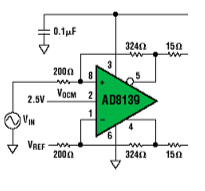
\includegraphics[scale = 0.8]{Esempio di OpAmp con rete circuitale.png}
\end{figure}

Al contrario, il segnale digitale può essere elaborato con un microprocessore o un DSP (Digital Signal Processor), 
cioè un dispositivo dedicato alla elaborazione numerica. \newline 

\subsection{Analogico vs Digitale: reiezione ai disturbi}
\footnote{Slide della prof | SDME 3.Conversione AD e Convertitori - Parte I | pag 10 \\  
Appunti | 2025-03-18 | pag 4}

Il segnale digitale ha una maggiore reiezione ai disturbi di quello analogico perchè 
il valore analogico ha infiniti valori, invece il segnale digitali ha valori finiti e "consentiti". \newline 

\newpage 

\section{Conversione analogico - digitale}
\footnote{Slide della prof | SDME 3.Conversione AD e Convertitori - Parte I | pag 11 \\  
Appunti | 2025-03-18 | pag 4}

La conversione AD (in inglese ADC: Analog to Digital Conversion) si attua con tre fasi in successione: 

\begin{enumerate}
    \item Campionamento 
    \item Quantizzazione 
    \item Codifica
\end{enumerate}

Il campionamento, partendo da un segnale analogico come il seguente: 

\begin{figure}[h]
    \centering
    \includegraphics[scale = 0.6]{Esempio segnale analogico.png}
\end{figure}

si può applicare il campionamento. \newline 

Il campionamento attua la discretizzazione dell'asse dei tempi e si definiscono gli istanti di campionamento equi-spaziati tra loro, quindi non si ha una perdita di informazione. \newline 

Il segnale campionato, da quello analogico, diventerà: 

\begin{figure}[h]
    \centering
    \includegraphics[scale = 1]{Segnale analogico campionato.png}
\end{figure}


Una volta che il segnale è stato campionato, lo si quantizza. \newline 

Per quantizzazione si intende la discretizzazione delle ampiezze, quindi una perdita di informazione. \newline 

Il segnale quantizzato diventerà: 

\begin{figure}[h]
    \centering
    \includegraphics[scale = 1]{Segnale quantizzato.png}
\end{figure}

Una volta quantizzato, il segnale viene codificato. \newline 

Per codifica si intende che viene assegnato a ciascun livello di quantizzazione una parola di codice, 
usualmente binaria, univocamente determinata. \newline 

Il segnale codificato diventerà: 

\begin{figure}[h]
    \centering
    \includegraphics[scale = 1]{Segnale codificato.png}
\end{figure}

\newpage 

Dal punto di vista misuristico, le fasi più interessanti sono le prime due: campionamento e quantizzazione. \newline 

\newpage 

\section{Teorema fondamentale del campionamento}
\footnote{Slide della prof | SDME 3.Conversione AD e Convertitori - Parte I | pag 12 \\  
Appunti | 2025-03-18 | pag 4 -5}

Per il campionamento, è stato rivoluzionario il teorema del campionamento scritto dal matematico 
Claude. \newline 

Di seguito il teorema fondamentale del campionamento: 

\begin{figure}[h]
    \centering
    \includegraphics[scale = 0.5]{Teorema fondamentale del campionamento originale.PNG}
\end{figure}

\begin{tcolorbox}
    Shannon pubblicò il suo teorema nella seguente rivista: 
    "Claude E. Shannon Communication in the Presence of Noise
Proceedings of the IRE, vol. 37, no. 1, pp. 10-21, Jan. 1949" 
consultabile al seguente link \\ \url{https://webusers.imj-prg.fr/~antoine.chambert-loir/enseignement/2020-21/shannon/shannon1949.pdf}
\end{tcolorbox}

Visto che il teorema è stato pubblicato nel 1949, alcune terminologie sono diverse da quello al giorno d'oggi. \newline 

Le seguenti terminologie sono: 

\begin{itemize}
    \item cps è un'abbreviazione di cycles per second, nei giorni odierni utilizziamo l'indicazione di Hz 
    \item per ordinates si intendono i valori istantanei 
\end{itemize}

La traduzione italiana, con i seguenti adattamenti, del teorema fondamentale del campionamento è la seguente: \newline 

Se la funzione f(t) contiene nessuna frequenza maggiore di W Hz, è completamente determinata dai 
suoi valori istantanei spaziati da una serie di punti spaziati di $\frac{1}{2W}$ secondi tra di loro. \newline 

Questo teorema ci dice che, se gli istanti di campionamento sono opportunamente individuati, 
la funzione che si ottiene andando a prelevare il valore istantaneo del segnale solo in quegli istanti è completamente determinata, quindi non si ha perdita di informazione. \newline 

\newpage 

\section{La Delta di Dirac e il campionamento}
\footnote{Slide della prof | SDME 3.Conversione AD e Convertitori - Parte I | pag 13 - 14 \\  
Appunti | 2025-03-18 | pag 5}

Il teorema di Shannon fa riferimento ai valori istantanei (le ordinate) della funzione, 
prelevati in corrispondenza degli istanti di campionamento. \newline 

Per prelevare un segnale in un singolo istante, matematicamente, si ricorre alla funzione Delta di Dirac. \newline 

Se bisogna svolgere il campionamento in tutti gli istanti della funzione, bisogna applicare la seguente formula:

{
    \Large 
    \begin{equation}
        g_s (t) = g(nT) \cdot \sum_{n = - \infty}^{+ \infty} \delta (t - nT)
    \end{equation}
}

ovvero, un "treno" di Delta di Dirac, cioè una Delta di Dirac shiftata al valore nT della funzione. \newline 

\begin{tcolorbox}
    Il tema lo ho già approfondito nei miei appunti di Teoria dei segnali nel capitolo 
    1.3 Delta di Dirac \\\url{https://github.com/ciccio25/appunti-teoria-dei-segnali/blob/main/Appunti%20Teoria%20dei%20segnali.pdf} .\newline 

    Di seguito il capitolo: \newline

La Delta di Dirac gode di queste proprietà: 

{
    \Large 
    \begin{equation}
        \begin{cases}
            \delta (t = 0) = \infty \\ \\
            \delta (t \not = 0) = 0 \\ \\
            \int_{- \infty}^{ \infty} \delta (t) dt = 1
        \end{cases}
    \end{equation}
}

$\int_{- \infty}^{ \infty} \delta (t) dt = 1$ indica che l'area della Delta di Dirac è unitaria. \newline 

Se l'area è diversa da uno, basta moltiplicare la Delta di Dirac per un coefficiente moltiplicativo A. \newline 

La Delta di Dirac può trovarsi anche in un istante diverso da zero: 

{
    \Large 
    \begin{equation}
        t_0 \not = 0 
        \rightarrow 
        \delta (t - t_0)
     \end{equation}
}

o, in altri termini, possiamo vederla come una delta di Dirac shiftata nel tempo $t_0$. \newline 

Grazie alla Delta di Dirac shiftata nel tempo $t_0$, possiamo svolgere un campionamento ideale di un segnale s(t) all'instante $t_0$ come: 

{
    \Large 
    \begin{equation}
        \int_{- \infty}^{\infty} 
        s(t) \delta (t - t_0) dt 
        = 
        s(t_0)
    \end{equation}
}

\end{tcolorbox}

Non esiste un segnale fisico reale che si comporta come la delta di Dirac a causa delle sue proprietà che tendono ad infinito. \newline 

Possiamo grafitare la Delta di Dirac come: 

\begin{figure}[h]
    \centering
    \includegraphics[scale = 0.15]{Dirac_distribution_PDF.png}
\end{figure}


\newpage 

Da un punto di vista misuristico, la Delta di Dirac non ci aiuta perchè rappresenta solo un modello matematico, 
che non ha riscontri nei circuiti e nei segnali reali. \newline 

D'altra parte, Shannon, nel suo teorema non menziona mai la Delta di Dirac, ma ci dice che dobbiamo prendere i valori istantanei della funzione f(t). \newline 

\newpage 

\section{Fase 1: Campionamento}
\footnote{Slide della prof | SDME 3.Conversione AD e Convertitori - Parte I | pag 15 - 17 \\  
Appunti | 2025-03-18 | pag 6}

Per adattare e applicare il campionamento nell'ambito delle misure, dobbiamo applicare il teorema di Shannon e applicarlo con segnali reali. \newline 

Campionare un segnale analogico g(t) significa, sotto l'aspetto operativo, 
individuare la successione dei valori $g(t_0 + nT_c)$ dove $t_0$ è un istante iniziale arbitrario, 
n è un intero e $T_c$ è la quantità costante chiamata periodo di campionamento, in particolari istanti, detti "istanti di campionamento", 
temporaneamente equi-spaziati. \newline 

Dalla successione dei valori individuata mediante il campionamento è possibile, secondo il teorema del campionamento, 
ricavare univocamente il segnale analogico g(t) se il segnale g(t) rispetta le seguenti proprietà: 

\begin{enumerate}
    \item g(t) deve avere banda limitata 
    \item il tempo che separa due successivi istanti di campionamento è minore di un valore critico stabilito dalle caratteristiche del segnale analogico 
    \item si acquisiscono 2x infiniti campioni
\end{enumerate}

Riguardo al primo punto, se si considera un segnale reale con infinite frequenze, 
è possibile applicare un filtraggio, ma bisogna valutare se le frequenze che il filtro toglie sono importanti per la nostra trattazione. \newline 

L'ultima condizione riguardo agli infiniti valori, è impossibile da mettere nella pratica. \newline 

\begin{tcolorbox}
    Regola aurea del mondo reale: è difficile o quasi impossibile avere infiniti valori
\end{tcolorbox}

Per campionare il segnale analogico g(t) senza perdere informazione, 
il periodo di campionamento $T_c$, cioè la distanza temporale fra due successivi campioni, deve essere: 

{
    \Large 
    \begin{equation}
        T_c < \frac{1}{2B}
    \end{equation}
}

dove B è la banda del segnale determinata dalla frequenza più alta che si trova nel suo spettro (lo si può notare dalla serie di Fourier del segnale). \newline 

Quindi, si può applicare il campionamento solo per segnali a banda limitata. \newline 

Definiamo la frequenza di campionamento $f_c$ l'inverso del tempo di campionamento $T_c$: 

{
    \Large 
    \begin{equation}
        f_c = \frac{1}{T_c}
    \end{equation}
}

La frequenza di campionamento $f_c$ deve essere:

{
    \Large 
    \begin{equation}
        f_c > f_N 
    \end{equation}
}

dove: 

{
    \Large 
    \begin{equation}
        f_N = 2B
    \end{equation}
}

$f_N$ prende il nome di frequenza di Nyquist. \newline 

La frequenza di Nyquist varierà in base alla banda del segnale in esame. \newline 

\newpage 

\subsection{Fase 1: Campionamento e aliasing (prima parte)}
\footnote{Slide della prof | SDME 3.Conversione AD e Convertitori - Parte I | pag 18 - 20 \\  
Appunti | 2025-03-18 | pag 6 - 7}

\begin{tcolorbox}
    Nota a lezione: aliasing è un termine latino, quindi si legge all'italiana
\end{tcolorbox}

Consideriamo un segnale sinusoidale nel tempo. \newline 

Se campioniamo a una frequenza di campionamento $f_c$: 

{
    \Large 
    \begin{equation}
        f_c = 8B
    \end{equation}
}

il campionamento individuerà i seguenti punti nel segnale: 

\begin{figure}[h]
    \centering
    \includegraphics[scale = 0.6]{Frequenza di campionamento a 8B.png}
\end{figure}

Questa sinusoide passa per i punti (quelli che nella figura sono di colore rosso) individuati, quindi è univocamente determinata. \newline 

Considerando una frequenza di campionamento $f_c$ : 

{
    \Large 
    \begin{equation}
        f_c = 4B
    \end{equation}
}

il campionamento individuerà i seguenti punti nel segnale: 

\begin{figure}[h]
    \centering
    \includegraphics[scale = 0.6]{Frequenza di campionamento a 4B.png}
\end{figure}

Come il caso precedente della frequenza di campionamento a 8B, 
a questa frequenza di campionamento 
questa sinusoide passa per i punti (quelli che nella figura sono di colore rosso) individuati, quindi è univocamente determinata. \newline 

Se consideriamo la frequenza di campionamento $f_c$ esattamente: 

{
    \Large 
    \begin{equation}
        f_c = 2B
    \end{equation}
}

il campionamento può trovare questi due casi: 

\begin{figure}[h]
    \centering
    \includegraphics[scale = 0.6]{Frequenza di campionamento a 2B caso 1.png}
    \includegraphics[scale = 0.6]{Frequenza di campionamento a 2B caso 2.png}
\end{figure}

\newpage 

Rispetto ai casi della frequenza di campionamento maggiore di 2B, 
in questo caso, possiamo trovare infinite funzioni che possono passare per i punti individuati: 
per questo motivo si dice che esiste un errore di alias. \newline 

Se campioniamo a frequenza esattamente uguale al doppio della banda, 
non siamo in grado di individuare univocamente la funzione che passa per quei punti. \newline 

Shannon, nel suo teorema del campionamento, aveva scritto che, per campionare, bisognare ricavare univocamente il segnale analogico. \newline 

In questo caso, non essendo univocamente identificata una funzione dopo il campionamento,  
troviamo infinite funzioni alla stessa frequenza, ma diversa ampiezza. \newline 

Considerando il caso peggiore, cioè campionando ad una frequenza di campionamento minore di 2B, ad esempio: 

{
    \Large 
    \begin{equation}
        f_c = 1.33B
    \end{equation}
}

il segnale campionato potrà essere:

\begin{figure}[h]
    \centering
    \includegraphics[scale = 0.6]{Frequenza di campionamento a 1,33B caso 1.png}
\end{figure}

Interpolando i punti: 

\begin{figure}[h]
    \centering
   \includegraphics[scale = 0.6]{Frequenza di campionamento a 1,33B caso 2.png}
\end{figure}


Il segnale in viola è una possibile funzione che interpola i punti della funzione campionata, 
che è, come si nota dalla figura, un segnale sotto-campionato. \newline 

Dalle figure dei segnali sotto-campionati, si può formalizzare la seguente osservazione: 
se si riduce la frequenza di campionamento $f_c$ sotto al limite di Shannon, non si è più in grado di individuare univocamente 
la frequenza della funzione originale. \newline 

\newpage 

\section{Fase 1: Campionamento (seconda parte)}
\footnote{Slide della prof | SDME 3.Conversione AD e Convertitori - Parte I | pag 21 - 25 \\  
Appunti | 2025-03-18 | pag 7 - 8}

Considerando una frequenza di campionamento $f_c$ maggiore di quella di campionamento, 
si evita l'incongruenza di alias. \newline 

Se si riesce a rispettare questa condizione, 
NON si ha perdita di informazione nella fase di campionamento .\newline 

Considerando il segnale originale analogico, come in figura: 

\begin{figure}[h]
    \centering
    \includegraphics[scale = 0.6]{Esempio segnale analogico.png}
\end{figure}

il segnale è a tempo-continua e la vogliamo rendere a tempo-discreta. \newline 

Il primo passo è il seguente: 

\begin{figure}[h]
    \centering
    \includegraphics[scale = 1]{Segnale analogico moltiplicato per la funzione di campionamento.png}
\end{figure} 

Come si nota dalla figura, si moltiplica il segnale analogico per una funzione di campionamento di impulsi istantanei che ha l'andamento mostrato (quelli con il palloncino blu): 
essa è definita solo in corrispondenza degli istanti di campionamento e in quegli istanti il suo valore è unitario. \newline 

Questo funzione di campionamento NON è la Delta di Dirac, è un'altra funzione, perchè, nella Delta di Dirac l'ampiezza negli istanti $T_c$ tende a infinito. \newline 

Facendo il prodotto tra il "treno di impulsi unitario" e la funzione analogica da campionare, 
si ha la seguente funzione: 

\begin{figure}[h]
    \centering
    \includegraphics[scale = 1]{Segnale analogico campionato.png}
\end{figure} 

Come si nota dalla figura, tra un valore e l'altro (tra i due puntini rossi) la funzione non è definita in quegli istanti. \newline 

Sapendo dal corso di Segnali Determinati Aleatori che c'è una relazione tra tempo e frequenza tra due funzioni, 
se si fa una moltiplicazione nel tempo, allora in frequenza ci sarà una convoluzione tra i due segnali. \newline 

In frequenza il segnale analogico sarà:

\begin{figure}[h]
    \centering
    \includegraphics[scale = 0.6]{Esempio segnale analogico.png}
    \includegraphics[scale = 0.6]{Banda del segnale analogico da campionare.png}
\end{figure}

\newpage 

Dallo spettro di frequenza (figura a destra), 
notiamo che la banda del segnale analogico B è minore della frequenza di campionamento $f_c$, 
e che la frequenza di campionamento $f_c$ è maggiore della frequenza di Nyquist $f_N$ relativo al segnale. \newline 

Se si considera il segnale di campionamento, avremo una riga in presenza di $f_c$: 

\begin{figure}[h]
    \centering
    \includegraphics[scale = 1]{Segnale di campionamento in frequenza.png}
\end{figure} 

Facendo la circonvoluzione in frequenza tra il segnale analogico con banda B e il segnale degli impulsi unitari, 
avremo il seguente caso: 

\begin{figure}[h]
    \centering
    \includegraphics[scale = 1]{Convoluzione in frequenza tra generico segnale e treno di impulsi unitari.png}
\end{figure} 

\newpage 

Come avete studiato nel corso di Segnali Determinati Aleatori, 
la convoluzione genera delle repliche del segnale analogico originale per ogni $n f_c$ dove n è un numero intero. \newline 

Utilizzato un filtro come il seguente (denotato e tratteggiato di verde):

\begin{figure}[h]
    \centering
    \includegraphics[scale = 0.6]{Convoluzione in frequenza tra generico segnale e treno di impulsi unitari con filtro realizzabile.png}
\end{figure} 

si può ricavare il segnale originale in banda base. \newline 

Non essendo un filtro ripido, è realmente realizzabile. \newline 

Se invece si dilata il tempo e si pone: 

{
    \Large 
    \begin{equation}
        f_c = f_N
    \end{equation}
}

e facendo la convoluzione, avremo il seguente caso: 


\begin{figure}[h]
    \centering
    \includegraphics[scale = 0.6]{Convoluzione in frequenza tra generico segnale e treno di impulsi unitari con filtro NON realizzabile.png}
\end{figure} 

In questo caso, come indicato dalla linea tratteggiata verde, per recuperare il segnale campionato in banda base, 
il filtro è ideale e non fisicamente realizzabile. \newline 

Avremo un caso peggiore, quando: 

{
    \Large 
    \begin{equation}
        f_c < B
    \end{equation}
} 

e lo possiamo visualizzare nella seguente figura: 

\begin{figure}[h]
    \centering
    \includegraphics[scale = 1]{Convoluzione in frequenza tra generico segnale e treno di impulsi unitari al di sotto di B.png}
\end{figure} 

Come dimostrato da questi casi, 
il caso migliore per campionare un segnale senza avere aliasing è quello di: 

{
    \Large 
    \begin{equation}
        \begin{split}
            f_c &> 2B
            \\ 
            &\updownarrow
            \\ 
            T_c &< \frac{1}{2B}
        \end{split} 
    \end{equation}
}

cioè come possiamo visualizzare nel primo caso della convoluzione. \newline 

Più differenza c'è tra $f_c$ da $f_N$, tanto meno gravoso sarà il progetto del filtro passa-basso che bisognerà usare. \newline 

Una regola a "spanna" è quella di stare almeno a 20\% in più rispetto alla banda B per poter ricostruire il segnale 
con un LPF reale. \newline 

Campionando a una frequenza al di sotto di $f_N$, non avremo mai modo di recuperare il segnale originale perchè la convoluzione genera un segnale non lineare. \newline 

\newpage 

\section{Fase 2: Quantizzazione}
\footnote{Slide della prof | SDME 3.Conversione AD e Convertitori - Parte I | pag 26 - 30 \\  
Appunti | 2025-03-18 | pag 9 - 11}

Dalla conversione analogico-digitale, l'obbiettivo del campionamento, cioè la discretizzazione nel tempo del segnale, 
è quello di discretizzare anche le ampiezze del segnale analogico, quindi dobbiamo quantizzare il segnale campionato. \newline 

Quantizzare significa creare una divisione nelle ampiezze del segnale. \newline 

Per quantizzare il segnale campionato si deve, per prima cosa, fissare il campo di misura, 
cioè un intervallo di valori compreso fra un minimo ed un massimo: 
in altre parole dobbiamo individuare l'escursione massima del segnale. \newline 

Le scelte usuali per il campo di misura, se si considera come grandezza i volt, sono due: 

\begin{itemize}
    \item campo unipolare, cioè con estremi tra 0 ed $E_c$ volt 
    \item campo bipolare, cioè con estremi $-E_c$ e $+E_c$ volt (l'intervallo sarà simmetrico) 
\end{itemize}


Dopo aver stabilito il campo di misura, 
lo si suddivide in un numero arbitrario finito di intervalli contigui, cioè "uno dietro all'altro". \newline 

Gli intervalli possono essere di due tipi: 

\begin{itemize}
    \item intervalli di uguale ampiezza, si tratterà di quantizzazione uniforme 
    \item intervalli di ampiezza diversa, si tratterà di quantizzazione non uniforme
\end{itemize}

Consideriamo, per adesso, la quantizzazione uniforme. \newline 

Dopo aver stabilito il campo di misura e averlo diviso in N intervalli contigui, come in figura: 

\begin{figure}[h]
    \centering
    \includegraphics[scale = 1]{Divisione del campo bipolare.png}
\end{figure} 

bisogna individuare gli N valori del centro di ciascun intervallo in cui è stato suddiviso il campo di misura. \newline 

Nella figura, gli intervalli sono indicati con le linee grigie, 
invece il centro degli intervalli è indicato con le linee tratteggiate in rosso. \newline 

Considerando il caso in cui avremo un segnale quantizzato, 
avremo il seguente caso:

\begin{figure}[h]
    \centering
    \includegraphics[scale = 1]{Campo bipolare con campioni da quantizzare.png}
\end{figure} 

\newpage 

Se consideriamo i puntini blu il segnale campionato, 
questo ultimo viene assegnato al valore centrale dell'intervallo 
più vicino, che è, appunto il puntino rosso. \newline 

A causa di questo "spostamento", nella quantizzazione, a differenza del campionamento, 
si ha una perdita dell'informazione originale. \newline 

Essendoci una perdita di informazione, si introduce una incertezza di quantizzazione. \newline 

Ogni valore quantizzato rappresenta l'ampiezza del valore campionato a meno di un valore $\pm \frac{e}{2}$. \newline 

Per ridurre l'entità di incertezza, dobbiamo ridurre il valore di e, cioè l'ampiezza degli intervalli di quantizzazione. \newline 

Ridurre il valore di e, non signfica modificare il campo, cioè modificare l'intervallo tra $[-E_c, + E_c]$, 
significa aumentare i livelli di quantizzazione. \newline 

La quantizzazione porta ad una alterazione del segnale: il valore originale del segnale nell'istante di campionamento 
viene alterato di una quantità che risulta, al massimo, pari alla semi-ampiezza dell'intervallo in cui esso cade. \newline 

Questa alterazione è chiamata incertezza di quantizzazione e, 
con campo bipolare e quantizzazione uniforme in N intervalli, vale: 

{
    \Large 
    \begin{equation}
        \begin{split}
            \Delta g 
            &= 
            \pm \left( \frac{2 E_c}{N}\right) \frac{1}{2}
            \\ 
            &= \pm \frac{2 E_c}{2N}
            \\
            &= \pm \frac{E_c}{N}
        \end{split}
    \end{equation}
}

Questo è un errore che possiamo calcolare prima di svolgere una misura. \newline 

La quantizzazione è una funzione univoca e non biunivoca: 

\begin{figure}[h]
    \centering
    \includegraphics[scale = 0.8]{Quantizzazione funzione univoca.PNG}
\end{figure} 

\newpage

Essendoci un errore, la quantizzazione distorce il segnale originale: l'obbiettivo è rendere la distorsione la più piccola possibile. \newline 

Dalla formula di $\Delta g$, a parità di campo di misura, N è il parametro che definisce l'incertezza di quantizzazione. \newline 

Inoltre N influenza anche la codifica: ogni intervallo dovrà essere dotato di codifica univoca. \newline 

L'aumento dei livelli di quantizzazione significa anche avere maggiori bit, 
che serviranno per la codifica del segnale. \newline 

\newpage 

\subsection{Fase 2: Quantizzazione non silenziata}
\footnote{Slide della prof | SDME 3.Conversione AD e Convertitori - Parte I | pag 31 - 32 \\  
Appunti | 2025-03-18 | pag 11 | 2025-03-19 | pag 2}

Campionando un segnale nullo a cui è sovrapposto un rumore anche minimo, si avrebbero valori quantizzati non nulli e molto diversi l'uno dall'altro. \newline 

Come si nota dalle seguenti figure: 

\begin{figure}[h]
    \centering
    \includegraphics[scale = 0.45]{Rumore dopo che si è quantizzato in una quantizzazione non silenziata.png}
\end{figure} 

il rumore viene esaltato e sembra venire meno la capacità di reiezione al rumore dei segnali digitali. \newline 

\newpage 

\subsection{Fase 2: Quantizzazione silenziata}
\footnote{Slide della prof | SDME 3.Conversione AD e Convertitori - Parte I | pag 33 - 34 \\  
Appunti | 2025-03-19 | pag 2}

Per evitare l'amplificazione del rumore, si può applicare la quantizzazione silenziata dove esiste un intervallo "centrato" sul valore nullo, come si vede in figura: 

\begin{figure}[h]
    \centering
    \includegraphics[scale = 0.45]{Da quantizzazione non silenziata a quantizzazione silenziata.png}
\end{figure} 

Grazie a questa scelta, lo zero volt è un livello di quantizzazione e quindi 
il rumore, che generalmente cade nell'intervallo "colorato in blu celestino", viene centrato a zero. \newline 

Grazie alla quantizzazione silenziata, si avrà una reiezione al disturbo perchè il rumore deve avere un'intensità non trascurabile per manifestarsi sul segnale. \newline 

A differenza della quantizzazione non silenziata, se esiste un disturbo con densità trascurabile si avrà il seguente caso: 

\begin{figure}[h]
    \centering
    \includegraphics[scale = 0.45]{Rumore dopo che si è quantizzato in una quantizzazione silenziata.PNG}
\end{figure} 

Inoltre, quando i valori del segnale campionato arrivano ai livelli di campo, 
cioè $-E_c$ e $+E_c$, non vengono neanche elaborati e/o presi in considerazione dal quantizzatore. \newline 

\newpage 

\section{Fase 2: Quantizzazione - conclusioni}
\footnote{Slide della prof | SDME 3.Conversione AD e Convertitori - Parte I | pag 35 \\  
Appunti | 2025-03-19 | pag 2}

Al termine della fase 2 della conversione da analogico a digitale, quindi alla fine della quantizzazione, 
si ha un segnale discretizzato sia nei tempi che nelle ampiezze perchè può assumere solo un numero limitato di valori, quelli individuati dagli intervalli di quantizzazione. \newline 

Quindi, dal segnale analogico, si è passati al segnale campionato, al segnale quantizzato: 

\begin{figure}[h]
    \centering
    \includegraphics[scale = 0.45]{Esempio segnale analogico.png} 
    \\
    \includegraphics[scale = 0.8]{Segnale analogico campionato.png}
    \\
    \includegraphics[scale = 0.8]{Segnale quantizzato.png}
\end{figure} 

Per concludere, la scelta dell'ADC si baserà su: 

\begin{itemize}
    \item frequenza di campionamento $f_c$ 
    \item risoluzione
\end{itemize}

\newpage 
\chapter{Conversione AD e convertitori - parte II}

\begin{figure}[h]
    \centering
    \includegraphics[scale = 1]{Sample And Hold e Track And Hold.png}
\end{figure}

\newpage 

\section{Fase 3: codifica}
\footnote{Slide della prof | SDME 3.Conversione AD e Convertitori - Parte II | pag 4 \\  
Appunti | 2025-03-25 | pag 2 - 3}

Dopo il campionamento e la quantizzazione, 
il segnale ha bisogno di essere codificato. \newline 

Per codifica si intende il processo che associa univocamente a ciascuno dei valori 
corrispondenti ai centri degli N intervalli in cui è stato suddiviso il campo di misura 
una "parola" (in questo caso) binaria a M bit. \newline 

È necessario che ciascuno degli N valori quantizzati disponga di una "sua" parola. \newline 

Siccome non ci devono essere codifiche doppie è richiesto che: 

{
    \Large 
    \begin{equation}
        N \le 2^{M}
    \end{equation}
}

La scelta ottimale della codifica va fatta rispetto al livello di tensione e dei dispositivi che devono rielaborare il segnale. \newline 

Questo corso non tratterà della scelta ottimale della codifica, 
bensì tratteremo esclusivamente della mappatura ottimale per la quantizzazione silenziata, 
essendo quella che garantisce reiezione al disturbo. \newline 

\newpage 

\section{Mappatura ottimale per la quantizzazione silenziata}
\footnote{Slide della prof | SDME 3.Conversione AD e Convertitori - Parte II | pag 5 - 8 \\  
Appunti | 2025-03-25 | pag 3}

Avendo un campo di misura simmetrico, cioè da $-E_c$ e $+E_c$, 
per ottenere una quantizzazione silenziata bisogna avere un numero dispari  di intervalli. \newline 

Consideriamo quindi: 

{ 
    \Large 
    \begin{equation}
        N = 2^{M} - 1
    \end{equation}
}

Siccome si considera un numero di N che è minore di $2^{M}$, 
l'incertezza di quantizzazione sarà maggiore. \newline 

L'errore di quantizzazione e sarà: 

{
    \Large 
    \begin{equation}
        e = \frac{2 E_c}{2^{M} -1}
    \end{equation}
}

Se consideriamo N dispari e una quantizzazione silenziata, 
i livelli di quantizzazioni graficati saranno del tipo: 

\begin{figure}[h]
    \centering
    \includegraphics[scale = 0.8]{Quantizzazione silenziata con N livelli dispari.png}
\end{figure}

Avere N dispari complicherebbe le operazioni in binario, 
che invece sarebbero semplici se N fosse una potenza di 2. \newline 

Si parte da una quantizzazione non silenziata, e poi si traslano tutti gli intervalli in basso di mezzo livello. \newline 

Con questo shift, dalla figura precedente, otteniamo la seguente figura: 

\begin{figure}[h]
    \centering
    \includegraphics[scale = 0.8]{Quantizzazione silenziata con N livelli dispari shiftata.png}
\end{figure}

\newpage 

Si ottiene un intervallo centrato nello zero e i rimanenti intervalli di quantizzazione ottenuti 
dividendo il campo di misura da $-E_c$ a $+E_c$ in $2^{M}$ parti. \newline 

Disponendo di M bit per la codifica, avremo che: 

{
    \Large 
    \begin{equation}
        \begin{cases}
            N \leq 2^{M}
            \\
            N = 2^{M} 
            \\  
            e = \frac{2 E_c}{N}
        \end{cases}
    \end{equation}
}

Ma così facendo, abbiamo creato due intervalli (quelli evidenziati in giallo) 
che non andremo ad usare e presentano ampiezze diverse perchè non sono uniformi 
rispetto agli altri livelli di quantizzazione. \newline 

Di seguito la stessa figura, ma con maggiori considerazioni scritte a lezione: 

\begin{figure}[h]
    \centering
    \includegraphics[scale = 0.5]{Quantizzazione silenziata con N livelli dispari shiftata con appunti pag 6.png}
\end{figure}

Di seguito la tecnica di quantizzazione effettivamente usata negli ADC commerciali. \newline 

I due intervalli segnati in giallo, apparentemente "persi", possono essere usati per segnalare due condizioni di errore: 

\begin{itemize}
    \item condizione di overflow, quando il segnale di ingresso arriva al limite superiore del campo di misura (cioè l'intervallo giallo di $+E_c$) 
    \item condizione di underflow, quando il segnale di ingresso ha valore troppo basso, prossimo al limite inferiore del campo di misura (cioè l'intervallo giallo di $-E_c$)
\end{itemize}

In tutti gli altri intervalli non in giallo, essendo equi-spaziati e costanti, l'incertezza sarà costante in ciascun intervallo. \newline 

Supponendo un esempio con i seguenti valori: 

{
    \Large 
    \begin{equation}
        \begin{split}
            M &= 8 
            \\ 
            &\downarrow 
            \\
            N &= 2^{M} 
            \\ 
            &= 2^{8}
            \\
            &= 256
        \end{split}
    \end{equation}
}

Questo significa che il livello minimo 0000 0000 e quello massimo 1111 1111 saranno usati per segnalare 
le condizioni di, rispettivamente, underflow e overflow. \newline 

I rimanenti 254 livelli, saranno utilizzati per codificare il segnale. \newline 

\newpage 

\section{La conversione A/D reale}
\footnote{Slide della prof | SDME 3.Conversione AD e Convertitori - Parte II | pag 9 \\  
Appunti | 2025-03-25 | pag 4} 

Dopo aver spiegato cosa significa svolgere un campionamento, 
di seguito sarà presentato un esempio di architettura di campionatore. \newline 

Il campionatore che analizzeremo è quello del Sample and Hold, Track and Hold. \newline 

Da un punto di vista ideale, possiamo rappresentarlo così: 

\begin{figure}[h]
    \centering
    \includegraphics[scale = 0.8]{Sample and Hold e Track and Hold ideale.png}
\end{figure}

I componenti principali di un "Sample and Hold" (compattato come S \& H) sono: 

\begin{itemize}
    \item due OpAmp connessi come inseguitore di tensione, quindi il circuito presenterà un guadagno unitario 
    \item un MOS-FET che opera come interruttore 
    \item un condensatore C che opera come memoria 
\end{itemize}

La scelta del valore del condensatore C sarà cruciale per il S \& H. \newline 

\newpage 

\section{Sample and hold: funzionamento ideale}

\subsection{Ipotesi di componenti ideali} 
\footnote{Slide della prof | SDME 3.Conversione AD e Convertitori - Parte II | pag 10 \\  
Appunti | 2025-03-25 | pag 2 - 4} 

Ipotizziamo i componenti dell'S \& H ideali, cioè: 

\begin{itemize}
    \item gli OpAmp avranno impedenza infinita in ingresso e impedenza nulla in uscita 
    \item il mosfet sarà a perfetta conduzione o perfetta interdizione perchè si comporterà da interruttore 
    \item il condensatore è una capacità ideale in cui la la carica che si immagazzina non si dissipa, cioè non ci sono correnti di fuga, e si scarica istantaneamente
\end{itemize}

Siccome consideriamo un Mos-FET come interruttore, il circuito da: 

\begin{figure}[h]
    \centering
    \includegraphics[scale = 0.8]{Sample and Hold e Track and Hold ideale.png}
\end{figure}

passerà a: 

\begin{figure}[h]
    \centering
    \includegraphics[scale = 0.8]{Sample and Hold e Track and Hold ideale con interruttore.png}
\end{figure}

\newpage 

\subsection{Interruttore chiuso} 
\footnote{Slide della prof | SDME 3.Conversione AD e Convertitori - Parte II | pag 11 - 14\\  
Appunti | 2025-03-25 | pag 4 - 5} 

Consideriamo il caso in cui l'interruttore venga chiuso, grazie al segnale alto di Sample 
dal pin $S-\overline{H}$. \newline 

Il circuito diventerà: 

\begin{figure}[h]
    \centering
    \includegraphics[scale = 0.5]{Sample and Hold e Track and Hold ideale con interruttore abbassato con note.png}
\end{figure}

Se l'interruttore è chiuso, essendo l'AmpOp in configurazione inseguitore, 
la tensione che si ha nel nodo rosso $v_{x} (t)$ la si avrà anche nel nodo rosa (segnato con il cerchio 1). \newline 

Essendo l'interruttore, cioè il Mos-fet, chiuso, la tensione $v_{x} (t)$ va a caricare il condensatore C, 
il quale si porta ad una tensione $v_c$ uguale a $v_x$ (nodo verde). \newline 

Il secondo OpAmp a destra ha ingresso $v_c$ (nodo verde), è in configurazione non invertente, 
quindi $v_{out} (t)$ (nodo blu) ha la stessa tensione di $v_c (t)$. \newline 

Ipotizzando che in questo momento $v_x(t)$ abbia l'andamento di una rampa, possiamo graficare $v_x (t)$, che è uguale a $v_{out} (t)$ 
e il segnale di enable del $S-H$ come: 

\begin{figure}[h]
    \centering
    \includegraphics[scale = 0.8]{Segnale ingresso e di uscita del S&H e del segnale di enable.png}
\end{figure}

Ad un istante di tempo arbitrario, il sistema viene interdetto: 
portando al livello basso il segnale che pilota l'interruttore, si apre:  

\begin{figure}[h]
    \centering
    \includegraphics[scale = 0.4]{Da track a hold nell'S&H interruttore.png}
\end{figure}

Il circuito a sinistra si definisce come "S \& H in track-mode" (track perchè l'andamento di $v_{out} (t)$ è uguale a quello di $v_x (t)$), 
il circuito a destra, cioè con l'interruttore alto, si definisce come "S \& H in hold-mode" (hold perchè si cercherà di mantenere $v_{out} (t)$ costante uguale a $v_x (t)$ nell'istante $t_0$ 
dove $t_0$ è il momento in cui si alza l'interruttore). \newline 

La tensione di ingresso può variare arbitrariamente, ma, poiché l'interruttore è aperto, 
la variazione della tensione $v_x$ non raggiunge la seconda parte del circuito, 
cioè la parte del circuito a destra dell'interruttore. \newline 

Le tempistiche di track e hold devono rispettare le condizioni di Shannon-Nyquist. \newline 

Ora che l'interruttore è aperto, l'AmpOp a destra non seguirà più la tensione di $v_x (t)$, 
bensì quella del condensatore $v_c (t)$. \newline 

Siccome si considera un condensatore C ideale, le cariche accumulate sulla capacità non possono "sfuggire" perchè: 

\begin{itemize}
    \item verso sinistra il circuito è aperto (resistenza infinita) 
    \item verso destra, l'impedenza di ingresso dell'OpAmp ideale è infinita (concetto della massa virtuale spiegato precedentemente) 
    \item le armature sono perfettamente isolate, quindi le cariche restano nel condensatore e mantengono la tensione $v_c (t)$ ad un valore costante, che aveva nell'istante $t_0$ in cui l'interruttore è stato aperto
\end{itemize}

Ripetendo che anche l'AmpOp a destra è in configurazione non invertente, durante la fase di hold, $v_{out} (t)$ sarà uguale a $v_c (t)$ 
che, idealmente, rimane costante. \newline 

Utilizzando le figure: 

\begin{figure}[h]
    \centering
    \includegraphics[scale = 0.7]{hold time per S&H.png}
\end{figure}

in cui: 

\begin{itemize}
    \item la funzione blu è l'andamento di $v_{out}$ 
    \item la funzione rossa è l'andamento di $v_x$, che nell'istante di hold può variare arbitrariamente 
    \item il segnale $S - \overline{H}$ è a livello basso, quindi avviene la fase di hold
\end{itemize}

Aprendo l'interruttore all'istante di campionamento, 
mantengo il segnale di uscita al valore che il segnale di ingresso aveva proprio in quell'istante e do il tempo ai circuiti successivi 
all'S \& H di effettuare quantizzazione e codifica. \newline 

Una volta che si è effettuato quantizzazione e codifica, bisogna ripetere i processi svolti precedentemente, 
ma questa volta per un nuovo istante di tempo. \newline 

Quindi, dalla fase di hold, bisogna ripassare alla fase di track (che dall'inglese significa inseguimento). \newline 

Graficando i grafici di $v_x$, $v_{out}$ e dell'enable pin $S - \overline{H}$: 

\begin{figure}[h]
    \centering
    \includegraphics[scale = 0.8]{track-hold-track nell'S&H.png}
\end{figure}

Come si nota dal grafico di $v_{out}$ (funzione in blu), idealmente tra il tempo di hold al tempo di track, 
la tensione $v_{out}$ diventa uguale a quella di $v_x$. \newline 

Quindi ritorniamo al caso precedente dove, nel periodo di track: 

{
    \Large 
    \begin{equation}
        v_x = v_{out} = v_c
    \end{equation}
}

La tensione ai capi del condensatore si porta rapidamente (idealmente lo fa in maniera istantanea) 
al livello della tensione $v_x$ erogato in uscita dall'inseguitore (primo OpAmp) e altrettanto rapidamente la tensione $v_{out}$ 
si porta al suo livello, eseguendo così una nuova fase di track. \newline 

A un certo punto $t_1$ arriva un nuovo istante di campionamento, l'interruttore si apre di nuovo e si segue la fase 
di mantenimento (hold) e il processo hold-track e track-hold si ripete. \newline 

Tutto questo processo, da un punto di vista ideale, è molto semplice perchè i componenti si comportano istantaneamente e idealmente. \newline 

\newpage 


\section{Sample and Hold: funzionamento reale} 
\footnote{Slide della prof | SDME 3.Conversione AD e Convertitori - Parte II | pag 15 - 29 } 

\subsection{L'acquisition time sull'S\&H reale} 
\footnote{Slide della prof | SDME 3.Conversione AD e Convertitori - Parte II | pag 15 - 16 \\  
Appunti | 2025-03-25 | pag 5 - 6} 

Nel S \& H ideale avevamo visto che tra la fase di hold-track, 
$v_{out}$ (funzione blu) insegue subito la tensione di ingresso $v_x$ (funzione rossa) come in figura: 


\begin{figure}[h]
    \centering
    \includegraphics[scale = 0.8]{track-hold-track nell'S&H.png}
\end{figure}

MA, nella realtà non avviene ciò. \newline 

\begin{tcolorbox}
    Nella realtà non esiste tutto subito e infinito. Altra regola aurea
\end{tcolorbox}

Nella realtà, il grafico delle tensioni del circuito saranno le seguenti: 

\begin{figure}[h]
    \centering
    \includegraphics[scale = 0.8]{tensioni in un S&H reale.png}
\end{figure}

Il nuovo elemento è l'acquisition time. \newline 

L'acquisition time è quel tempo che, nel mondo reale, 
è la somma tra il tempo che serve al primo Amp-Op per riportarsi al livello di $v_x$ 
dovuto alla resistenza non nulla di uscita dell'inseguitore definito come transitorio di carica 
e la resistenza non nulla del MOS-FET. \newline 

L'acquisition time può essere visto anche come un tempo di ritardo tra l'istante in cui si attiva 
la fase di track e l'istante in cui la tensione $v_c (t)$ aggancia la $v_x$. \newline 

Essendo $v_c (t)$ la tensione ai capi di un condensatore, 
$v_c (t)$ sale con andamento esponenziale, in questo caso smorzato 
perchè, dopo l'acquisition time,  $v_c = v_x$. \newline 

Dall'elettrotecnica, la costante di tempo con cui la tensione cresce dipende dal valore della capacità C scelta. \newline 

Quindi, per questo motivo, se si vuole mantenere basso l'acquisition time, bisogna avere un valore di C più basso possibile. \newline 

Non si può avviare una nuova fase di campionamento fino a che la tensione ai capi del condensatore non ha agganciato la $v_x$: 
questa fase si definisce come acquisition time esaurito. \newline 

Con tutte queste considerazioni, rispetto al mondo ideale, l'intervallo di campionamento 
non sarà uguale al tempo di hold, bensì alla somma tra il tempo di hold e l'acquisition time. \newline 

In formule: 

{
    \Large 
    \begin{equation}
        \begin{split}
            t_\text{campionamento ideale} &\le t_\text{campionamento reale}
            \\
            &\downarrow
            \\
            t_{hold} &\le t_{hold} + t_\text{acquisition time}
        \end{split}
    \end{equation}
}

Si può osservare che parte del valore del tempo di campionamento $T_c$, 
dato dal teorema di Shannon-Nyquist, dipende dalla rapidità dei circuiti di quantizzazione e codifica, 
e una parte dipende dal sample-and-hold. \newline 


\newpage 

\subsection{L'effetto delle ricombinazioni delle cariche sul S \& H reale} 
\footnote{Slide della prof | SDME 3.Conversione AD e Convertitori - Parte II | pag 17 - 19 \\  
Appunti | 2025-03-25 | pag 6} 

Consideriamo il caso del circuito S \& H ideale: 

\begin{figure}[h]
    \centering
    \includegraphics[scale = 0.8]{S&H ideale con cariche del condensatore.png}
\end{figure}

Considerando ideale i componenti, il condensatore C accumula le cariche (indicate di rosso) ai capi delle sue armature per sempre. \newline

Considerando invece il circuito S \& H reale, possiamo modellarlo in questa maniera: 

\begin{figure}[h]
    \centering
    \includegraphics[scale = 1]{S&H reale con cariche del condensatore.png}
\end{figure}

Rispetto al circuito ideale, è presente anche una resistenza parassita $R_p$. \newline 

\begin{tcolorbox}
    Piccola guida alla notazione utilizzata dalla prof: 
    \begin{itemize}
        \item $R_p$ con la R maiuscola si intende una resistenza parassita che, idealmente, dovrebbe essere la più grande possibile 
        \item $r_p$ con la r minuscola si intende una resistenza parassita che, idealmente, dovrebbe essere la più piccola possibile
    \end{itemize}
\end{tcolorbox}

Si modella questa resistenza parassita $R_p$ in parallelo al condensatore C per rappresentare il fenomeno delle ricombinazione delle cariche. \newline 

In questo caso, per ricombinazione delle cariche si intende che, se idealmente le cariche dovrebbero rimanere ai capi delle armature del condensatore C, 
nella realtà si disperdono nel circuito (e generalmente sotto forma di calore) per i seguenti motivi del mondo reale: 

\begin{itemize}
    \item l'impedenza di ingresso dell'OpAmp a destra di C è elevata ma non è infinita 
    \item l'isolamento tra le armature del condensatore C è elevato ma non è infinito 
    \item anche in interdizione, cioè quando il MOS-FET idealmente dovrebbe essere un interruttore aperto, nella realtà lascia passare una debolissima corrente
\end{itemize}


In fase di hold, le cariche del condensatore C, anziché rimanere sulle armature, 
passano da una armatura all'altra tramite la $R_p$, come mostrato nelle seguenti figure: 

\begin{figure}[h]
    \centering
    \includegraphics[scale = 1]{S&H reale con cariche del condensatore scarica 1.png}
    \\
    \includegraphics[scale = 1]{S&H reale con cariche del condensatore scarica 2.png}
    \\
    \includegraphics[scale = 1]{S&H reale con cariche del condensatore scarica 3.png}
    \\
    \includegraphics[scale = 1]{S&H reale con cariche del condensatore scarica 4.png}
\end{figure}

\newpage

quindi si ha la scarica del condensatore. \newline 

Dall'elettrotecnica e sapendo che in parallelo a C c'è una resistenza $R_p$, la tensione ai capi di C non resta costante, 
ma segue un esponenziale decrescente. \newline 

Da un punto di vista grafico, si passerà dal grafico delle tensioni del circuito ideale: 

\begin{figure}[h]
    \centering
    \includegraphics[scale = 0.4]{S&H ideale interruttore aperto.PNG}
    \includegraphics[scale = 0.6]{hold time per S&H.png}
\end{figure}

al grafico delle tensioni nel circuito reale: 

\begin{figure}[h]
    \centering
    \includegraphics[scale = 1]{S&H reale con cariche del condensatore scarica 4.png}
    \includegraphics[scale = 1]{S&H reale tensioni hold time.png}
\end{figure}

Poiché tutte le impedenze che danno origine alla $R_p$ e che sono dovute alle non idealità dei componenti 
e anche alle anomalie delle giunzioni, non sono costanti, si preferisce (come al solito) semplificare la trattazione 
e considerare la scarica con andamento lineare anziché esponenziale decrescente. \newline 

Dall'elettrotecnica, si può stimare la pendenza della curva esponenziale come: 

{
    \Large 
    \begin{equation}
        \tau = RC
    \end{equation}
}

\newpage 

\subsection{Droop rate (velocità di discesa della tensione)} 
\footnote{Slide della prof | SDME 3.Conversione AD e Convertitori - Parte II | pag 20 - 21 \\  
Appunti | 2025-03-25 | pag 6 - 7} 

Come scritto precedentemente, piuttosto che calcolarci l'andamento esponenziale della scarica del condensatore, 
si cerca di linearizzarlo perchè è più semplice per i calcoli. \newline 

\begin{tcolorbox} 
    Linearizzare la pendenza della retta di $\tau = RC$ causa una sovrastima dell'entità della scarica, 
    ma sovrastimare è meglio perchè sicuramente funzionerà meglio il progetto
\end{tcolorbox}

Allora, dall'andamento esponenziale decrescente, si sceglierà di passere al seguente andamento lineare della tensione di $V_{out}$ e quindi di $V_c$. \newline 

Partendo dall'andamento esponenziale, calcoliamo l'angolo $\alpha$

\begin{figure}[h]
    \centering
    \includegraphics[scale = 1.5]{Droop rate nel S&H reale.png}
\end{figure}

Da $\alpha$ si calcola il droop rate come: 

{
    \Large 
    \begin{equation}
        \tan(\alpha) = \text{Droop rate}
    \end{equation}
}

Il droop rate esprime la pendenza della curva di scarica del condensatore nella fase iniziale. \newline 

Si considera che la scarica prosegua sempre con quella pendenza. \newline 

La tangente dell'angolo $\alpha$ è il droop rate, la velocità di discesa della tensione. \newline 

Il droop rate dipende dalla resistenza parassita $R_p$, che consente la ricombinazione delle cariche. \newline 

La corrente che passa sulla $R_p$ è legata alla tensione $v_c(t)$ e non alla capacità. \newline 

Se dovessi raddoppiare la capacità, la corrente si manterrebbe invariata perchè essa dipende da $v_c (t)$. \newline 

Allora, se io aumentassi la capacità del condensatore, la corrente circolante sulla $R_p$ rimarrebbe invariata, 
ma, si rallenterebbe molto il processo di diminuzione della tensione $v_c(t)$. \newline 

Nella realtà, la $R_p$ è una resistenza non lineare. \newline 

Aumentando C, si riduce il droop rate perchè aumentano il numero di cariche accumulate. \newline 

\newpage 

\subsection{Droop voltage} 
\footnote{Slide della prof | SDME 3.Conversione AD e Convertitori - Parte II | pag 22 - 23 \\  
Appunti | 2025-03-25 | pag 7} 

Aumentando la durata di fase di hold, aumenta il droop: spiegato diversamente, la tensione iniziale si riduce. \newline 

Il droop considerato accettabile negli ADC deve essere inferiore della metà dell'ampiezza dell'intervallo di quantizzazione perchè 
la tensione $v_{out}(t_0)$ deve rimanere nel bin (cestino) dell'intervallo di quantizzazione. \newline 

Le figure spiegano meglio il processo appena introdotto: 

\begin{figure}[h]
    \centering
    \includegraphics[scale = 1]{Scelta del droop rate negli ADC.png}
\end{figure}

Tipicamente, i costruttori di ADC mettono a disposizione un PIN sul quale collegare un condensatore 
col valore di capacità stabilito in funzione dei requisiti del progetto, quindi si ha fisicamente lo stesso S \& H 
ma per diversi tempi di track e hold. \newline 

Per la non linearità di $R_p$, si cerca di linearizzarlo con la seguente formula: 

{
    \Large 
    \begin{equation}
            \text{droop voltage} [t_0, t] = \text{droop rate} \cdot (t - t_0)
    \end{equation}
}

in cui la dimensione del droop voltage è il volt. \newline 

Inoltre $t-t_0$ dipende dalla scelta del tempo di elaborazione dell'ADC. \newline 

Fissando il droop voltage, si può calcolare C e quindi anche $t-t_0$. \newline 

\newpage 

\subsection{Sottrazione di cariche} 
\footnote{Slide della prof | SDME 3.Conversione AD e Convertitori - Parte II | pag 24 \\  
Appunti | 2025-03-25 | pag 7} 

Per sottrazione di carica si intende il momento in cui si porta in fase di hold il dispositivo 
e si nota una brusca variazione della tensione di uscita, 
dovuto al cross-talk tra la linea di Enable dell'S \& H e le altre linee dell'S \& H. \newline 

Confrontando i segnali ideali (a sinistra) e i segnali reali (a destra) dovuto alle sottrazioni di cariche: 

\begin{figure}[h]
    \centering
    \includegraphics[scale = 0.55]{Tensioni dell'S&H dovuto alla sottrazione di cariche.png}
\end{figure}


L'ampiezza dovuta alla sottrazione di cariche è chiamato hold step o pedestal. \newline

\newpage 

\subsection{Hold step o pedestal} 
\footnote{Slide della prof | SDME 3.Conversione AD e Convertitori - Parte II | pag 25 - 28 \\  
Appunti | 2025-03-25 | pag 8} 

\begin{figure}[h]
    \centering
    \includegraphics[scale = 1]{Pedestal.png}
\end{figure}

L'hold step o pedestal è determinato dalla non idealità del circuito S \& H perchè tra Gate e Drain del MOS-FET reale sussiste una capacità parassita, 
come si può vedere in figura: 

\begin{figure}[h]
    \centering
    \includegraphics[scale = 1]{Capacità parassita mosfet sample and hold.png}
\end{figure}

Durante la fase di track, la capacità parassita deve essere caricata in questo modo: 
il gate deve essere positivo rispetto al drain, quindi la capacità parassita ha le cariche negative sul lato superiore 
e positive sull'armatura opposta del condensatore C di memoria. \newline 

Il condensatore C di memoria usato nel S \& H ha, ai suoi capi, ha una tensione positiva. \newline 

Nell'istante in cui viene cambiato lo stato del gate e il MOSFET si interdice (cioè idealmente diventa un interruttore aperto), 
la tensione del gate deve diventare negativa rispetto alla tensione del drain. \newline 

Quindi, la capacità parassita deve invertire la polarità: per fare ciò, si carica delle cariche positive del condensatore di memoria C, 
come mostrato in figura: 

\begin{figure}[h]
    \centering
    \includegraphics[scale = 1]{Capacità parassita mosfet sample and hold si carica dal condensatore di memmoria.png}
\end{figure}

Dopo che ciò si è svolto, le cariche positive e negative nei due circuiti si presentano in questa maniera: 

\begin{figure}[h]
    \centering
    \includegraphics[scale = 1]{Capacità parassita mosfet sample and hold dopo che si è caricato dal condensatore di memmoria.png}
\end{figure}

\newpage

Per ridurre il pedestal, si può: 

\begin{itemize}
    \item mettere un MOSFET con capacità parassita estremamente piccola 
    \item aumentare il valore della capacità di memoria C molto superiore rispetto alla capacità parassita
\end{itemize}

La formula per calcolare il pedestal è la seguente: 

{
    \Large 
    \begin{equation}
        \text{pedestal} = \frac{1}{C}
    \end{equation}
}

dove le dimensioni del pedestal sono i volt. \newline 

Dalla formula si può notare che il pedestal è il reciproco del condensatore C di memoria. \newline 

\newpage 

\subsection{Banda passante} 
\footnote{Slide della prof | SDME 3.Conversione AD e Convertitori - Parte II | pag 29 \\  
Appunti | 2025-03-25 | pag 8} 

Un altro elemento parassita presente in un S \& H reale è una resistenza parassita $R_p$ in serie all'OmAmp e al MOSFET, 
proprio perchè questi due componenti presentano una resistenza idealmente nulla, ma che nella realtà è presente. \newline 

Possiamo rappresentarla con questa nuova resistenza parassita $R_p$: 

\begin{figure}[h]
    \centering
    \includegraphics[scale = 1]{Resistenza parassita nell'OpAmp.png}
\end{figure}

Questa $R_p$ è difficile da stimare. \newline 

Facendo uno "zoom" del circuito dopo il Mosfet e prima del secondo OpAmp, 
il circuito sarà proprio una resistenza in serie al condensatore C di memoria: 

\begin{figure}[h]
    \centering
    \includegraphics[scale = 0.8]{Filtro passa basso.png}
\end{figure}

Visualizzando il circuito R e C in Fourier, è proprio un filtro passa-basso dove la frequenza di taglio è: 

{
    \Large 
    \begin{equation}
        f_t = \frac{1}{2 \pi RC}
    \end{equation}
}

Se il segnale di ingresso $v_x (t)$ avesse una frequenza superiore rispetto alla frequenza di taglio del filtro passa-basso, 
le sue evoluzioni non si vedrebbero in uscita perchè sarebbero eliminate e / o attenuate dal filtro. \newline 

La banda passante è: 

{
    \Large 
    \begin{equation}
        \text{banda passante} = \frac{1}{C}
    \end{equation}
}

cioè è inversamente proporzionale alla capacità del condensatore di memoria. \newline 

\newpage

\section{Sample and Hold reale e capacità di memoria}
\footnote{Slide della prof | SDME 3.Conversione AD e Convertitori - Parte II | pag 30 \\  
Appunti | 2025-03-25 | pag 9}

Per riassumere, la scelta del valore del condensatore di memoria C del Sample and Hold influisce sui seguenti parametri: 

\begin{figure}[h]
    \centering
    \includegraphics[scale = 0.5]{Valore di C di memoria nel Sample and Hold reale.PNG}
\end{figure}

Il costruttore di S \& H non assume una decisione, ma lascia a noi utilizzatori la scelta della capacità di memoria da collegare, 
che sia più adatta per la nostra specifica applicazione. \newline 

Per aiutarci in questa scelta, il costruttore ci fornisce dei grafici di questi quattro parametri che varieranno in base al valore di C, che rappresentano il comportamento reale del dispositivo. \newline 

\newpage 


\chapter{Conversione AD e convertitori - parte III}

\begin{figure}[h]
    \centering
    \includegraphics[scale = 1]{FLASH ADC.png}
\end{figure}

\newpage 

\section{Convertitori A / D}
\footnote{Slide della prof | SDME 3.Conversione AD e Convertitori - Parte III | pag 3 \\  
Appunti | 2025-03-28 | pag 2 - 3}

Il problema maggiore della conversione del segnale analogico digitale è il tempo di elaborazione, 
che deve essere minore del tempo indicato nel teorema del campionamento. \newline 

Con l'avanzare della tecnologia, il tempo di elaborazione è diminuito grazie ad architetture di A/D sempre più sofisticate e più efficienti. \newline 

A rigore, ci dovrebbero essere due dispositivi dopo la quantizzazione del segnale: quantizzatori e poi codificatori, 
ma per semplicità li consideriamo insieme e prendono il nome di convertitori A/D. \newline

\newpage 

\section{Convertitori paralleli "Flash ADC"}
\footnote{Slide della prof | SDME 3.Conversione AD e Convertitori - Parte III | pag 4 \\  
Appunti | 2025-03-28 | pag 4}

La prima tipologia di convertitori ADC sviluppati sono gli ADC Flash. \newline 

Un esempio di architettura ADC flash a 3 bit: 

\begin{figure}[h]
    \centering
    \includegraphics[scale = 0.8]{FLASH ADC.png}
\end{figure}

Sapendo che, per i motivi precedentemente elencati, svolgeremo una quantizzazione silenziata bipolare, 
tra $-E_c$ e $+E_c$, l'obbiettivo dell'architettura flash ADC è quello di dividere il campo di misura in un certo numero di intervalli contigui, 
individuando le frontiere tra questi. \newline 

Ad ogni campione si da il valore che corrisponde al valore centrale. \newline 

Analizzando il circuito del flash ADC, a sinistra notiamo che un campione di fem eroga una tensione pari a $2E_c$, che è proprio l'ampiezza del campo di misura bipolare. \newline 

$2E_c$ viene suddiviso in una rete di resistenze tutte uguali, tranne agli estremi. \newline 

$2E_c$ deve essere compatibile con il livello che bisogna misurare. \newline 

Le tensioni alle frontiere tra gli intervalli di quantizzazione sono le tensioni alle quali si trovano i nodi delle rete di resistenze. \newline 

Di seguito il circuito con gli appunti presi a lezione: 

\begin{figure}[h]
    \centering
    \includegraphics[scale = 0.6]{FLASH ADC con appunti.png}
\end{figure}

\newpage 

Il punto di forza di questa architettura è la semplicità concettuale perchè è composta solo da: 

\begin{itemize}
    \item una rete resistiva, per individuare le frontiere degli intervalli di quantizzazione 
    \item una rete di comparatori, per confrontare il valore della tensione di ingresso $v_x$ e la tensione di un nodo del resistore 
    \item una rete di codifica, che associa ad ognuna delle configurazioni di uscite dei comparatori una parola binaria in uscita in modo univoco
\end{itemize}

\newpage

\subsection{Flash ADC - Quantizzazione}
\footnote{Slide della prof | SDME 3.Conversione AD e Convertitori - Parte III | pag 7 - 8\\  
Appunti | 2025-03-28 | pag 5 - 8 }

\begin{figure}[h]
    \centering
    \includegraphics[scale = 0.5]{FLASH ADC.png}
\end{figure}

La tensione ad ogni nodo (rosso) viene portata in ingresso ad un comparatore (triangolini viola), 
il quale confronta la tensione del nodo e la tensione $v_x$ (campionata) da convertire. \newline 

Il comparatore analogico ci dice se il segnale posto ad uno dei due ingressi è maggiore di quello applicato all'altro ingresso. \newline 

Le uscite dei comparatori vengono messe in ingresso ad una rete di codifica. \newline 

La rete di codifica permette di avere in uscita una parola binaria (quella indicata nella figura con N), 
che rappresenta l'intervallo entro cui i comparatori hanno individuato che si trova la tensione $v_x$. \newline 

L'architettura flash ADC è veloce proprio perchè ogni comparatore lavora autonomamente. \newline 

Analizzando la figura dell'architettura di esempio, il campo di misura viene diviso in 8 intervalli, quindi la parola codificata in una parola di 3 bit perchè: 

{
    \Large 
    \begin{equation}
        \text{Numero intervalli} = 2^{3} = 8
    \end{equation}
}

La tensione ai capi della resistenza R è l'ampiezza dell'intervallo di quantizzazione, 
quindi è legata all'incertezza. \newline 

Teoricamente, per ridurre l'incertezza, bisognerebbe aggiungere più resistori in serie, in modo da suddividere il campo di misura 
in un maggior numero di intervalli. \newline 

Il Sample and Hold ha prelevato il livello di tensione $v_x$, ma non l'ha misurata: 
è compito dell'ADC codificare quel livello. \newline 

Supponiamo che $v_x$ si trova nel seguente intervallo (tra il punto 1 e il punto 2): 

\begin{figure}[h]
    \centering
    \includegraphics[scale = 0.5]{Flash ADC con Vx tra due resistori.PNG}
\end{figure}

$v_x$ è maggiore del valore di tensione al nodo 2 e minore del valore di tensione al nodo 1. \newline 

In formule: 

{
    \Large 
    \begin{equation}
        v_2 < v_x < v_1
    \end{equation}
}
Noi sappiamo che $v_x$ è compreso tra $v_1$ e $v_2$, ma non sappiamo quanto vale "realmente" $v_x$: 
se il nuovo $v_x ^{'}$ sarà compreso tra $v_1$ e $v_2$, dal codificatore uscirà la stessa parola di $v_x$. \newline 

Il comparatore collegato al nodo 2 avrà un'uscita a 1: 
l'ingresso invertente si trova a una tensione più bassa dell'ingresso non invertente. \newline 

Questo accade per tutti i comparatori "sotto" a questo, quindi avranno un'uscita al livello alto (cioè ad 1). \newline 

Il compratore collegato al nodo 1, avrà uscita a 0: 
la tensione in ingresso invertente è maggiore di quella all'ingresso non invertente. \newline 


La rete di codifica deve individuare qual è la posizione della frontiera tra le uscite a 1 le uscite a 0 dei comparatori, 
ovvero ha bisogno di individuare in quale intervallo si trova la tensione $v_x$ e fornisce in uscita una parola binaria che ne codifichi il valore in modo univoco. \newline 

\newpage 

\subsection{Flash ADC - codifica}
\footnote{Slide della prof | SDME 3.Conversione AD e Convertitori - Parte III | pag 9 - 10 \\  
Appunti | 2025-03-28 | pag 5 - 6, 8}

Considerando l'esempio: 

\begin{figure}[h]
    \centering
    \includegraphics[scale = 0.5]{Flash ADC con parola di esempio.png}
\end{figure}

La parola: 

{
    \Large 
    \begin{equation}
        N = 101
    \end{equation}
}

è la parola binaria che individua in modo univoco la tensione $v_x$. \newline 

Si può utilizzare qualsiasi tipo di codifica, quindi far corrispondere il livello di tensione $v_x$ a una parola di codice N. \newline 

In particolare, sono necessarie due parole di codice: 

\begin{itemize}
    \item una di overflow, che la rete di codifica può indicare con i bit tutti a uno (nell'esempio a 3 bit 111) 
    \item una di underflow, che la rete di codifica può indicare con i bit tutti a zero (nell'esempio a 3 bit 000)
\end{itemize}

Nell'architettura flash ADC non è presente un buffer di memoria, quindi l'ADC deve convertire il segnale sotto al tempo di campionamento. \newline 

Qualunque valore della $v_x$ che si trovi a cadere tra valori della tensione di riferimento individuati dai nodi 1 e 2 verrà ad assumere la stessa codifica 
e questo darà a luogo a perdita di informazione, che a sua volta comporterà incertezza di quantizzazione. \newline 

L'architettura flash, non solo è veloce, ha una estrema rapidità di conversione grazie ai suoi pochi componenti. \newline 

L'unico "collo di bottiglia", per quanto riguarda il tempo, dell'architettura flash è la rete di codifica. \newline 

Il tempo di conversione è denominato dalla latenza della rete di codifica e tale tempo è comunemente breve. \newline 

L'aspetto negativo dell'architettura flash ADC è una incertezza di quantizzazione relativamente elevata quando si deve suddividere il campo di misura in un numero molto elevato di intervalli. \newline 

Si ha questa incertezza di quantizzazione molto elevata perchè sono presenti molti resistori e ognuno di essi contribuisce all'incertezza di quantizzazione. \newline 

Inoltre, aumentare il numero di bit non è possibile perchè un ADC flash a 8 bit richiede una rete di 256 resistori e 255 comparatori. \newline 

Questi limiti tecnologici limitano le prestazioni in termini di incertezza, che non sono trascurabili. \newline 

\newpage 

\subsection{Flash ADC - Codifica errori OF e UF}
\footnote{Slide della prof | SDME 3.Conversione AD e Convertitori - Parte III | pag 11 - 12 \\  
Appunti | 2025-03-28 | pag 8}

Come scritto precedentemente, l'architettura Flash ADC è molto importante perchè la rete di codifica segnala quando 
è presente un underflow (UF) o un overflow (OF). \newline 

Come si nota dalla seguente figura: 

\begin{figure}[h]
    \centering
    \includegraphics[scale = 0.8]{Flash ADC con overflow.png}
\end{figure}

abbiamo un caso di overflow, cioè la tensione di ingresso $v_x$ supera quella del nodo del terzo resistore R. \newline 

Tutti i comparatori segnano un'uscita a livello alto (cioè 1). \newline 

La rete di codifica segnala un errore di conversione e di overflow, ad esempio con la parola 111. \newline 

Invece, analizzando un caso di underflow: 

\begin{figure}[h]
    \centering
    \includegraphics[scale = 0.8]{Flash ADC con underflow.png}
\end{figure}

succede il caso opposto dell'overflow. \newline 

La tensione di ingresso $v_x$ è al di sotto di quella minima. \newline 

Se la tensione $v_x$ è minore della tensione dell'ultimo nodo dell'ultimo resistore di valore $\frac{R}{2}$, 
allora la rete di codifica segnala la parola di underflow, ad esempio ponendo tutti i bit a 0. \newline 

Nel caso di esempio dei 3 bit, esiste UF con 000. \newline 

Come il caso dell'overflow, non sappiamo quando vale "realmente" $v_x$, sappiamo solo che è minore del campo di misura. \newline 


\newpage 

\subsection{Flash ADC: pro e contro}
\footnote{Slide della prof | SDME 3.Conversione AD e Convertitori - Parte III | pag 13 \\  
Appunti | 2025-03-28 | pag 8 - 9}

Per riassumere, di seguito i pro e i contro dell'architettura Flash ADC. \newline 

Il pro è la rapidità di conversione: generalmente è di 5 ns per 8 bit. \newline 

Il contro è l'elevata incertezza di quantizzazione, che è limitato dal numero di componenti da aggiungere, quindi il prezzo economico elevato 
dovuto all'aggiunta di ogni componente. \newline 

\newpage 

\section{Half-flash o semi-flash ADC}
\footnote{Slide della prof | SDME 3.Conversione AD e Convertitori - Parte III | pag 14 - 16 \\  
Appunti | 2025-03-28 | pag 9 - 10}

L'architettura Flash ha un enorme vantaggio, cioè la rapidità, ma ha un'elevata incertezza. \newline 

Per questo motivo, si è cercato di ovviare a ciò realizzando delle architetture più efficienti. \newline 

Gli ADC flash sono stati prima affiancati e poi sostituiti dai semi-flash. \newline 

Di seguito il block diagram di un half-flash ADC in commercio nel 1994: 

\begin{figure}[h]
    \centering
    \includegraphics[scale = 1]{Esempio di Half-flash ADC.PNG}
\end{figure}

Un half-flash è un convertitore flash con una tecnica modificata, evidenziata dai 3 blocchi. \newline 

I blocchi estremi (quelli cerchiati in blu e in giallo) sono due convertitori flash a 4 bit ognuno, quindi: 

{
    \Large 
    \begin{equation}
        4 \text{bit flash ADC} + 4 \text{bit flash ADC} = 8 \text{bit half-flash ADC} 
    \end{equation}
}

Questi due ADC flash sono poi collegati ad un convertitore digitale/analogico a 4 bit. \newline 

Questi tre componenti sono poi collegati ad una rete combinatoria con capacità di memoria, in questo caso con un buffer a 3 stati. \newline 

Possiamo schematizzare i tre componenti più importanti degli half-flash ADC anche in questa maniera: 

\begin{figure}[h]
    \centering
    \includegraphics[scale = 1]{Half-flash ADC architettura.png}
\end{figure}

\newpage 

Di seguito la spiegazione completa del processo di conversione considerando un half-flash a 8 bit. \newline 

Un primo convertitore A/D a 4 bit (quello di colore blu in figura)  fa una prima conversione grossolana del segnale già campionato 
che ha in ingresso, avendo solo 16 livelli di quantizzazione perchè: 

{
    \Large 
    \begin{equation}
        4 \text{ bit} = 2^{4} = 16 \text{ livelli di quantizzazione} 
    \end{equation}
}

I 4 bit generati dalla rete di codifica dell'ADC flash vengono portati in uscita e sono i 4 bit più significativi della parola di uscita (alche nel block diagram è indicato come 4 MSBs). \newline 

Questi 4 bit vengono mandati al buffer e al convertitore digitale / analogico (quello indicato in verde): 
la tensione generata dal DAC è il valore centrale dell'intervallo al quale il campione di segnale è stato convertito e quantizzato dal primo convertitore. \newline 

La tensione "ricostruita" dal DAC viene sottratta alla tensione analogica in ingresso (nodo di sottrazione di colore arancione in figura). \newline 

In uscita dal nodo differenza, troviamo quello che possiamo chiamare il resto della prima conversione, cioè la differenza tra il valore del segnale di ingresso da convertire e la tensione che corrisponde al punto centrale dell'intervallo, in cui esso è stato convertito. \newline 

Tale ingresso è messo in ingresso ad un secondo convertitore A / D a 4 bit (quello che in figura è di colore giallo), 
ma che ha un campo di misura limitato all'ampiezza di un intervallo di quantizzazione (a differenza del primo ADC che ha due intervalli di quantizzazione). \newline 

Il resto non potrà essere maggiore di $\pm$ la metà dell'intervallo di quantizzazione del primo ADC. \newline 

Il resto viene convertito fornendo i 4 bit meno significativi della parola in uscita: alche nel block diagram dell'half-flash di esempio, 
il secondo ADC è indicato con la dicitura 4 LSBs. \newline 


Questo schema di principio sembra contraddittorio: perchè mettere due ADC in cascata con un DAC in mezzo tra loro ? \newline 

Il motivo è che sia gli ADC flash che i DAC sono molto semplici da realizzare. \newline 

\newpage 


\subsection{DAC a scala di resistenze}
\footnote{Slide della prof | SDME 3.Conversione AD e Convertitori - Parte III | pag 17 \\  
Appunti | 2025-03-28 | pag 10}

\begin{tcolorbox}
    Lo schema del principio del DAC a scala di resistenze lo chiede all'esame con gli esempi dei valori numerici
\end{tcolorbox}


Di seguito lo schema di principio di un DAC a scala di resistenze a 4 bit: 

\begin{figure}[h]
    \centering
    \includegraphics[scale = 1]{DAC a scala di resistenze 4 bit.PNG}
\end{figure}

In linea di principio, un convertitore D/A a 4 bit può essere realizzato con la componentistica mostrata. \newline 

Occorre avere un campione di fem (quello a destra nella figura indicato con $E_c$), 
che può essere applicata agli ingressi della rete resistiva nel caso in cui i MOS-FET (quelli cerchiati in blu) siano in conduzione (cioè si comportano idealmente da interruttore chiuso) e gli altri MOS-FET (quelli cerchiati di rosso) siano interdetti (cioè idealmente si comportano da interruttori aperti). \newline 

Se il bit $b_3$ è 1, il MOS-FET collegato alla sua linea conduce, 
e la tensione $E_c$ viene portata al nodo verde evidenziato. \newline 

Per effetto dell'invertitore (c'è un not collegato in serie al MOSF-FET cerchiato in rosso ), 
il MOS-FET (cerchiato in rosso) è interdetto, cioè si comporta da interruttore aperto.\newline 

Se il bit $b_2$ è 0, la tensione $E_c$ non viene portata al nodo evidenziato in arancione perchè il MOS-FET (cerchiato in blu) è interdetto 
(cioè si comporta da interruttore aperto) e attraverso l'altro MOS-FET (quello cerchiato in rosso) è in conduzione (cioè si comporta da interruttore chiuso), 
quindi al nodo arancione viene portato a massa. \newline 

Ripetiamo il processo per i bit $b_1$ e $b_0$, allora la tensione finale viene portata all'OpAmp in modalità inseguitore, 
che "ripulisce" la tensione di ingresso e la manda a $v_{out}$. \newline 

$v_{out}$ potrà essere calcolata con la seguente formula: 

{
    \Large 
    \begin{equation}
        v_{out} 
        = 
        \frac{E_c}{2^{4}}
        \left( 
            2^{3} b_3 
            +
            2^{2} b_2
            +
            2^{1} b_1
            +
            2^{0} b_0
        \right)
    \end{equation}
}

Nel caso di esempio di una parola di codice 1000: 

\begin{figure}[h]
    \centering
    \includegraphics[scale = 1]{DAC a scala di resistenze 4 bit 1000.PNG}
\end{figure}

\newpage 

In questo caso numerico 1000: 

{
    \Large 
    \begin{equation}
        \begin{split}
        v_{out} 
        &= 
        \frac{E_c}{2^{4}}
        \left( 
            2^{3} b_3 
            +
            2^{2} b_2
            +
            2^{1} b_1
            +
            2^{0} b_0
        \right)
        \\ 
        &= 
        \frac{E_c}{2^{4}}
        \left( 
            2^{3} \cdot 1 
            +
            2^{2} \cdot 0
            +
            2^{1} \cdot 0
            +
            2^{0} \cdot 0
        \right)
        \\
        &= 
        \frac{E_c}{2^{4}} 
        \cdot
        2^{3}
        \\ 
        &= 
        \frac{E_c}{2} [V]
        \end{split}
    \end{equation}
}

\newpage 

\subsection{Half- flash ADC - pro e contro}
\footnote{Slide della prof | SDME 3.Conversione AD e Convertitori - Parte III | pag 18 - 19 \\  
Appunti | 2025-04-01 | pag 2 }

Come l'architettura Flash ADC, bisogna elencare i pro e i contro dell'architettura Half-flash ADC. \newline 

Il punto di forza è sicuramente la forte riduzione dei componenti fisici per realizzare l'half-flash. \newline 

Se consideriamo un ADC a 8 bit, per un flash-ADC a 8 bit sono necessari:

{
    \Large 
    \begin{equation}
        \begin{cases}
            2^{8} \text{ resistori } = 256 \text{ resistori }
            \\ 
            2^{8} - 1 \text{ comparatori } = 255 \text{ comparatori }
        \end{cases}
    \end{equation}
}

Invece, realizzando un half-flash ADC con 2 flash-ADC, un flash-ADC a 4 bit ha bisogno di: 

{
    \Large 
    \begin{equation}
        \begin{cases}
            2^{4} \text{ resistori } = 16 \text{ resistori }
            \\ 
            2^{4} - 1 \text{ comparatori } = 15 \text{ comparatori }
        \end{cases}
    \end{equation}
}

Moltiplicando per due i componenti per un half-flash a 8 bit: 

{
    \Large 
    \begin{equation}
        \begin{cases}
            16 \text{ resistori } \cdot 2 = 32 \text{ resistori }
            \\ 
            15 \text{ comparatori } \cdot 2 = 30 \text{ comparatori }
        \end{cases}
    \end{equation}
}

Invece il punto a sfavore dell'architettura half-flash è quello dell'aumento del tempo di conversione, dovuto all'effetto dei due "passi" in successione, in modo seriale. \newline 

A causa di questa caratteristica, gli half-flash non sono indicati per applicazioni in tempo reale. \newline 

Il tempo di conversione è la somma di tutti questi tempi perchè le operazioni viste vanno eseguite in cascata. \newline 

Gli half-flash erano adatti per applicazioni che non richiedevano elevate frequenze di campionamento, essendo meno costosi dei flash ADC. \newline 

Il compromesso da scegliere è o avere una maggiore risoluzione o aspettare, quindi avere una velocità di conversione maggiore. \newline 

La scelta dell'architettura half-flash ADC va fatta se siamo dispositi ad aspettare di più, rispetto agli ADC flash, a causa del maggior tempo di conversione, per avere in cambio una maggior risoluzione. \newline 

\newpage

\section{Two-stage pipelined flash Adc}
\footnote{Slide della prof | SDME 3.Conversione AD e Convertitori - Parte III | pag 20 \\  
Appunti | 2025-04-01 | pag 2 - 3}

Con il miglioramento della tecnologia, si è riusciti ad aumentare la frequenza di lavoro degli half-flash ADC, 
introducendo i "pipelined". \newline 

Di seguito lo schema del two-stage pipelined flash ADC: 

\begin{figure}[h]
    \centering
    \includegraphics[scale = 1]{Two-stage pipelined flash ADC.png}
\end{figure}

Rispetto alle architetture ADC viste precedentemente, cioè quella flash e quella half-flash, 
questo tipo di architettura è intermedia tra le due. \newline 

Rispetto all'architettura half-flash: 

\begin{figure}[h]
    \centering
    \includegraphics[scale = 0.6]{Half-flash ADC architettura.png}
\end{figure}


viene aggiunto un Sample and Hold (S \& H) supplementare: 
così facendo, una volta che il primo ADC (quello in blu) ha convertito un primo campione, 
esso può essere comandato a prelevare il campione successivo senza dover aspettare che gli altri blocchi terminino le proprie operazioni. \newline 

I tempi, rispetto all'architettura half-flash, diminuiscono visto che la modalità pipelined rende il primo ADC asincrono rispetto al resto dei blocchi circuitali. \newline 

Idealmente il DAC è istantaneo, nella realtà ha bisogno di tempo per assestarsi sulla tensione che deve emettere. \newline 

È un'architettura quasi parallela, perlopiù rimane seriale. \newline 

Il pro di utilizzare questa architettura è l'aumento del throughput (cioè la frequenza con cui si possono fornire i dati in uscita, e quindi della frequenza di campionamento) 
grazie alla strategia "pipeline". \newline 

Il contro è l'aumento della complessità circuitale di uno o più S \& H. \newline  


\newpage

\section{Multi-stage pipelined flash Adc}
\footnote{Slide della prof | SDME 3.Conversione AD e Convertitori - Parte III | pag 21 \\  
Appunti | 2025-04-01 | pag 3}

Aggiungendo più stadi al two-stage pipelined flash ADC si possono aumentare il numero di bit di risoluzione, ma diventa più complicato il circuito. \newline 

Di seguito uno schema di un Multi-stage pipelined flash Adc: 

\begin{figure}[h]
    \centering
    \includegraphics[scale = 0.7]{Multi-stage pipelined flash Adc.png}
\end{figure}

In figura una configurazione pipelined a 12 bit con i seguenti componenti: 

\begin{itemize}
    \item 3 ADC a 4 bit 
    \item 2 DAC 
    \item 2 S \& H
\end{itemize}

Rispetto al caso del two-stage pipelined flash ADC, bisogna aggiungere un altro S \& H, quindi il tempo di Hold dell'S \& H 
è molto importante. \newline 

I pro di questo tipo di architettura è l'ulteriore aumento del "throughput" rispetto all'architettura Two-stage pipelined flash Adc, 
e la riduzione di complessità rispetto a un flash ADC di uguale risoluzione. \newline 


Il contro è l'aumento del tempo di latenza a causa dei suoi tanti stadi di conversione. \newline 

Alche è consigliato questo tipo di architettura per applicazioni offline e non in tempo reale. \newline 

\newpage

\section{Convertitore a successive approssimazioni "SAR ADC"}
\footnote{Slide della prof | SDME 3.Conversione AD e Convertitori - Parte III | pag 23 - 24 \\  
Appunti | 2025-04-01 | pag 4 }

I convertitori a successive approssimazioni sono una famiglia di convertitori che segue un approccio opposto a quello visto finora. \newline

Se nei flash avevamo tanti comparatori per confrontare la tensione in ingresso con tutte le frontiere tra gli intervalli di quantizzazione, 
nei SAR ADC è presente un unico comparatore che confronta in maniera ciclica la tensione da convertire. \newline 

Ipotizzando di avere un campo di misura unipolare come in figura: 

\begin{figure}[h]
    \centering
    \includegraphics[scale = 1]{Campo unipolare.png}
\end{figure}

che va da 0 a $+E_c$ volt, suddiviso in un certo numero di intervalli uguali, si può realizzare un convertitore ad approssimazioni successive ad 8 bit come in figura: 

\begin{figure}[h]
    \centering
    \includegraphics[scale = 1]{SAR ADC a 8 bit.png}
\end{figure}

Un SAR ADC è composto dai seguenti elementi: 

\begin{itemize}
    \item un campione di fem che eroga una tensione $E_c$ 
    \item un convertitore D/A (quello colorato in verde) a 8 bit che eroga una tensione $v_r$ 
    \item un comparatore (quel triangolino in basso a sinistra della figura) che confronta la tensione generata dal DAC, cioè $v_r$ con la tensione $v_x$ che vogliamo convertire 
    \item un'unità logica di controllo (o abbreviata con ULC) che ha la capacità di determinare il valore di ciascuna delle, in questo caso, 8 linee 
    \item un clock che ha il compito di cadenzare lo svolgimento di un processo ciclico, che inizia quando viene mandato un segnale di start alla ULC 
\end{itemize}

Il metodo del SAR ADC è un metodo iterativo, in cui, ogni colpo di clock, si porta il segnale nel DAC. \newline 

\newpage 

\subsection{SAR ADC: funzionamento "ideale"}
\footnote{Slide della prof | SDME 3.Conversione AD e Convertitori - Parte III | pag 25 - 29 \\  
Appunti | 2025-04-01 | pag 4 - 5 }

Per la spiegazione, consideriamo un convertitore SAR a 4 bit, quindi $2^{4} = 16$ intervalli come in figura: 

\begin{figure}[h]
    \centering
    \includegraphics[scale = 0.4]{SAR ADC a 4 bit.png}
\end{figure}

Supponiamo che la tensione $v_x$ che deve essere convertita: 

\begin{figure}[h]
    \centering
    \includegraphics[scale = 0.4]{SAR ADC 1 step v_x.PNG}
\end{figure}

abbia il livello indicato in rosso, e cada dunque in quell'intervallo e sia superiore alla tensione $\frac{E_c}{2}$. \newline 

Quando si dà lo start (step molto importante che servirà anche nelle prossime architetture, perchè il processo di conversione inizia dal segnale di start) 
il primo passo che l'ULC esegue consiste nel portare ad 1 il bit più significativo che è in ingresso al DAC come si vede in figura: 

\begin{figure}[h]
    \centering
    \includegraphics[scale = 1]{SAR ADC 2 step v_x.PNG}
\end{figure}

Il DAC "reagisce" a questa situazione portando in uscita una tensione che è metà della tensione di $E_c$ che è al suo ingresso perchè $v_x$ è minore di $E_c$ : 

\begin{figure}[h]
    \centering
    \includegraphics[scale = 1]{SAR ADC 3 step v_x.PNG}
\end{figure}

\newpage 

Il comparatore confronta la tensione $v_x$ con il valore di uscita dal DAC: 
dal confronto, si vede che $v_x$ è maggiore di $\frac{E_c}{2}$: 

\begin{figure}[h]
    \centering
    \includegraphics[scale = 1]{SAR ADC 4 step v_x.PNG}
\end{figure}

Quindi viene portato ad 1 anche il secondo ingresso del DAC e aumenta di $\frac{E_c}{4}$ la tensione di $\frac{E_c}{2}$: 

\begin{figure}[h]
    \centering
    \includegraphics[scale = 1]{SAR ADC 5 step v_x.PNG}
\end{figure}

Ma la configurazione 1100 porta la tensione di uscita del DAC a $\frac{3}{4} E_c$ che è maggiore di $v_x$. \newline 

Allora, si spegne il secondo bit, si accende il terzo bit portando la tensione a $\frac{E_c}{2} + \frac{E_c}{8}$: 

\begin{figure}[h]
    \centering
    \includegraphics[scale = 1]{SAR ADC 6 step v_x.PNG}
\end{figure}

\newpage 

Si continua il processo che abbiamo indicato: 

\begin{figure}[h]
    \centering
    \includegraphics[scale = 1]{SAR ADC 7 step v_x.PNG}
\end{figure}

finché questi due casi si ripeteranno ciclicamente: 

\begin{figure}[h]
    \centering
    \includegraphics[scale = 1]{SAR ADC 8 step v_x.PNG}
    \\ 
    \includegraphics[scale = 1]{SAR ADC 9 step v_x.PNG}
\end{figure}

\newpage 

Quando la tensione dal DAC va sopra e sotto $v_x$, si dice che la tensione dal DAC si è stabilizzata. \newline 

Spetta poi all'ULC decidere come approssimare la tensione $v_x$. \newline  

Se starà sopra, si approssimerà $v_x$ per eccesso, se starà sotto, si approssimerà $v_x$ per difetto, 
quindi bisgognerà scegliere se porre a 1 o a 0 il LSB. \newline 

La scelta 

\begin{figure}[h]
    \centering
    \includegraphics[scale = 0.5]{SAR ADC step v_x finale.PNG}
\end{figure}

è una scelta possibile di $v_x$. \newline 

\newpage 

\subsection{SAR ADC: pro e contro}
\footnote{Slide della prof | SDME 3.Conversione AD e Convertitori - Parte III | pag 30 \\  
Appunti | 2025-04-01 | pag 5 }

Usando un solo comparatore e un DAC, con una tecnica ciclica di successive approssimazioni, si è individuato l'intervallo in cui si trova 
la tensione $v_x$, con una circuiteria relativamente semplice. \newline 

Il processo è ciclico, iterativo, e non si svolge in un solo colpo di clock come nel flash ADC: 
occorrono alcuni $\mu s$ per convertire un certo numero di bit. \newline 

Quindi è molto più lento di un flash ma ha risoluzione più elevata e incertezza di quantizzazione molto più piccola. \newline 

Le applicazioni tipiche sono le registrazioni audio. \newline

Le caratteristiche tipiche di un SAR ADC sono quelle di avere una risoluzione dai 16 ai 18 bit con una relativa lentezza di processione, circa 2 $\mu s$ per un SAR ADC a 16 bit. \newline 

\newpage 

\section{Cause di incertezza nei convertitori}
\footnote{Slide della prof | SDME 3.Conversione AD e Convertitori - Parte III | pag 31 - 32 \\  
Appunti | 2025-04-01 | pag 5 }

In questa sezione si elencheranno le cause di incertezza nelle architetture dei convertitori ADC studiate. \newline 

\textbf{Flash ADC} 

\begin{itemize}
    \item Incertezza di quantizzazione, che affligge tutti i convertitori 
    \item stabilità del campione di fem 
    \item la stabilità dei valori nominali dei singoli resistori 
    \item errori di linearità dovuta alla ripartizione dei valori di tensione tra i vari resistori 
    \item offset dei comparatori, che affligge soprattutto le misure di tensioni piccole 
\end{itemize}

\textbf{Semi-flash ADC} 

\begin{itemize}
    \item Incertezza di quantizzazione 
    \item stabilità dei campioni di fem contenuti nei convertitori ADC 
    \item errori di linearità del convertitore DAC 
    \item stabilità del campione fem del DAC 
    \item comportamento della giunzione che deve operare la differenza tra le tensioni
\end{itemize}

In genere, le ultime quattro cause, sono considerate trascurabili rispetto all'incertezza di quantizzazione, che è la principale causa di incertezza sia nei flash che negli Half-flash ADC. \newline 

\textbf{SAR ADC} 

\begin{itemize}
    \item Incertezza di quantizzazione 
    \item stabilità del campione di fem, che diventa instabile se la temperatura non è nel range in cui è stato tarato il fem 
    \item linearità del DAC 
    \item offset e la sensibilità del comparatore
\end{itemize}


\newpage 

\section{Convertitore ad inseguimento}
\footnote{Slide della prof | SDME 3.Conversione AD e Convertitori - Parte III | pag 33 \\  
Appunti | 2025-04-01 | pag 5 - 6 }

Un altro tipo di architettura di ADC è quella del convertitore ad inseguimento. \newline 

Partendo dall'architettura del SAR ADC: 

\begin{figure}[h]
    \centering
    \includegraphics[scale = 0.8]{SAR ADC a 8 bit.png}
\end{figure}

si può considerare un'ulteriore famiglia di convertitori, cioè quelli ad inseguimento. \newline 

Sostituendo l'unità logica di controllo con un contatore up-down: 

\begin{figure}[h]
    \centering
    \includegraphics[scale = 0.8]{Convertitore up-down.png}
\end{figure}

Ad ogni impulso di clock, il convertitore aggiorna il contatore, cioè il contenuto del suo registro, 
incrementandolo o decrementandolo di 1 dello stato della linea $U / \overline{D}$. \newline 

Il DAC ha in ingresso il valore totalizzato dal contatore. \newline 

\newpage 

\subsection{Principio di funzionamento}
\footnote{Slide della prof | SDME 3.Conversione AD e Convertitori - Parte III | pag 34 - 35 \\  
Appunti | 2025-04-01 | pag 6 | 2025-04-02 | pag 2 }

Vediamo cosa accade quando in ingresso a questo convertitore mettiamo una tensione non campionata da S \& H, ma con andamento di tipo analogico. \newline 

La tensione $v_x$ ha il seguente andamento: 

\begin{figure}[h]
    \centering
    \includegraphics[scale = 0.8]{Tensione analogica in ingresso al convertitore ad inseguimento.png}
\end{figure}

All'inizio il contatore ha uscita nulla, quindi il compratore che confronta la tensione che esce dal DAC con quella in ingresso $v_x$ 
avrà sempre uscita a livello alto. \newline 

Il contatore continuerà ad incrementare il proprio valore in uscita di 1 unità ogni colpo di clock. \newline 

La tensione in uscita dal DAC sale con un andamento a gradinata, 
fino a che non incrocia il valore della tensione analogica. \newline 

Adesso che il segnale $v_r$ si è agganciato a quello di $v_x$, $v_r$ varia di +1 o -1 in base l'andamento del segnale $v_x$: 

\begin{figure}[h]
    \centering
    \includegraphics[scale = 0.6]{andamento vr rispetto a vx.PNG}
\end{figure}

per questo motivo, nei convertitori ad inseguimento è consigliato un segnale analogico che non si modifica tanto in un breve periodo. \newline 

Il fatto di cambiare un solo bit alla volta, permette di avere una latenza estremamente bassa e una buona risoluzione perchè deriva dai SAR ADC. \newline 

La tecnica di alzare la frequenza di campionamento diventa strategica per ridurre il rumore di quantizzazione. \newline 

\newpage 

\subsection{Filtro numerico BB}
\footnote{Slide della prof | SDME 3.Conversione AD e Convertitori - Parte III | pag 36}

In un convertitore SAR convenzionale, il tempo di conversione è relativamente lungo. \newline 

Quindi la frequenza di campionamento $f_c$ non può essere molto elevata. \newline 

Come si vede dalla figura: 

\begin{figure}[h]
    \centering
    \includegraphics[scale = 0.4]{spettro dei segnali in un SAR ADC parte 1.PNG}
\end{figure}

$f_c$ sarà superiore alla frequenza di Nyquist $f_N$, ma non troppo alta. \newline 

Come abbiamo studiato a Teoria dei segnali con il mitico Chiaraluce, quando vado a campionare, 
ovvero si fa la convoluzione tra gli spettri, la prima replica dello spettro ha una frequenza minima pari a $f_c - B$: 

\begin{figure}[h]
    \centering
    \includegraphics[scale = 0.4]{spettro dei segnali in un SAR ADC parte 2.PNG}
\end{figure}

Se si vuole ricostruire il segnale di banda base (BB) dal segnale campionato, eliminando le repliche, 
il filtro BB ha requisiti molto stringenti perchè deve essere molto ripido: 

\begin{figure}[h]
    \centering
    \includegraphics[scale = 0.4]{spettro dei segnali in un SAR ADC parte 3.PNG}
\end{figure}

Invece, se si campiona un segnale ad una frequenza $f_c$ maggiore, ci sarebbe un "buco" in frequenza maggiore tra il segnale campionato (quello viola) e il segnale in BB (quello rosso). \newline 

\newpage 

\subsection{Filtro numerico BB con convertitore ad inseguimento}
\footnote{Slide della prof | SDME 3.Conversione AD e Convertitori - Parte III | pag 37 \\  
Appunti | 2025-04-02 | pag 3 }

Invece, campionando con un convertitore ad inseguimento, la frequenza di campionamento $f_c$ è nettamente più alta rispetto alla frequenza di Nyquist $f_N$, 
quindi c'è più spazio in frequenza tra la frequenza massima del segnale in BB e il segnale campionato. \newline 

Allora si può realizzare un filtro meno ripido rispetto al caso del SAR ADC. \newline 

Con le seguenti figure, si riassume quello che succede in frequenza con un convertitore ad inseguimento: 

\begin{figure}[h]
    \centering
    \includegraphics[scale = 0.6]{spettro dei segnali in un convertitore ad inseguimento.PNG}
\end{figure}

\newpage 

\subsection{Rumore di quantizzazione}
\footnote{Slide della prof | SDME 3.Conversione AD e Convertitori - Parte III | pag 38 - 39 \\  
Appunti | 2025-04-02 | pag 3 }

Per errore di quantizzazione si intende la differenza tra il valore della tensione da convertire (cioè il segnale reale) 
e il valore quantizzato che lo rappresenta. \newline 

Le considerazioni svolte saranno svolte quando il segnale campionato è arrivato a regime, trascurando il transitorio iniziale. \newline 

Considerano il segnale $\delta q$ come il segnale di rumore: 

\begin{figure}[h]
    \centering
    \includegraphics[scale = 0.6]{errore di quanrizzazione in un convertitore ad inseguimento.png}
\end{figure}

cioè la differenza tra segnale quantizzato e reale, che possiamo chiamare anche come rumore di quantizzazione. \newline  

Che frequenza ha $\delta q$ ? \newline 

Il rumore di quantizzazione ha un periodo che non supera il doppio del periodo di campionamento: 
o è uguale al periodo di campionamento nel transitorio, o è uguale al doppio nei tratti di segnale a regime. \newline 

Vedendolo in frequenza, se il rumore di quantizzazione ha un periodo: 

{
        \Large 
        \begin{equation}
            \begin{split}
            T_{noise} &\leq 2 T_c 
            \\
            &\updownarrow 
            \\
            f_{noise} &\ge \frac{f_c}{2}
            \end{split}
        \end{equation}
}

Quindi si può inserire un filtro numerico in uscita all'ADC per attenuare il rumore di quantizzazione: 

\begin{figure}[h]
    \centering
    \includegraphics[scale = 0.6]{filtro per recuperare il segnale in BB anche se esiste rumore di quantizzazione.PNG}
\end{figure}

\newpage 

L'intensità del rumore di quantizzazione (o rumore di campionamento) non ha effetto, visto che lo si può filtrare, 
quindi si possono realizzare anche dei convertitori grossolani, in cui tale rumore non sia trascurabile, 
perchè comunque lo si può filtrare: questo è il principio impiegato dai convertitori sigma-delta. \newline 

\newpage 

\section{Sigma-Delta $\Sigma - \Delta$}
\footnote{Slide della prof | SDME 3.Conversione AD e Convertitori - Parte III | pag 40 - 41 \\  
Appunti | 2025-04-02 | pag 3 - 5}

Lo schema a blocchi di un convertitore Sigma-Delta:

\begin{figure}[h]
    \centering
    \includegraphics[scale = 0.5]{Schema a blocchi convertitore Sigma Delta.PNG}
\end{figure}

Il blocco viola è un blocco integratore, che integra il residuo tra $v_x$ e quello che esce dal DAC. \newline 

Il concetto di questo convertitore è quello di codificare la variazione che il segnale esibisce tra campioni consecutivi. \newline 

Come si vede dallo schema del Sigma-Delta, è presente un comparatore (triangolo giallo), 
ma sulla retroazione è presente un DAC ad un solo bit, quindi grossolano. \newline 

Il filtro decimatore (quello in grigio) ha il compito di eliminare il rumore di quantizzazione in uscita. \newline 

Con questa architettura, si possono avere frequenze di campionamento molto alte, risoluzioni elevate con prezzi contenuti. \newline 


I convertitori Sigma-Delta sono quelli più usati oggigiorno, in particolare nell'ambito delle telecomunicazioni. \newline 

Sono basati su uno schema di principio che prevede il ricorso alle operazioni di sovra-campionamento (oversampling), 
quantization noise shaping, filtraggio digitale e decimazione. \newline 

Possiamo visualizzare i diversi schemi di architetture rispetto al rumore in frequenza con questi casi: 

\begin{figure}[h]
    \centering
    \includegraphics[scale = 0.8]{contributi dei componenti del sigma delta in frequenza.PNG}
\end{figure}

\newpage 

Il noise shaping è una tecnica che solo i circuiti digitali possono fare. \newline

In pratica il noise shaping prende la densità spettrale del rumore e poi lo spalma in tutta la banda. \newline 

In commercio, si possono trovare convertitori che integrano il campionatore, cioè il Sample and Hold. \newline 

\newpage 

\section{Limiti dei convertitori}
\footnote{Slide della prof | SDME 3.Conversione AD e Convertitori - Parte III | pag 43 - 47 \\  
Appunti | 2025-04-02 | pag 6 - 7}

Ogni convertitore è soggetto ad errori di conversione e limiti che derivano dalla quantizzazione della tensione: rumore elettrico, altre imperfezioni e non idealità dei componenti. \newline 

L'errore di quantizzazione può essere calcolato e limitato, ma mai del tutto eliminato. \newline 

Errori e limitazioni dovuti a non idealità sono propri di ogni specifico convertitore: 
una volta misurato l'errore, si può correggere l'effetto in seguito alla misura. \newline 

Un ADC, per ogni valore convertito, associa un errore limitato, pari a $\pm \frac{1}{2}$ LSB (Least Significant  Bit). \newline 

Lo scarto tra il valore d'ingresso e il valore digitalizzato presenta una distribuzione uniforme, perchè si considera ogni valore equiprobabile in quell'intervallo, 
chiamato passo di quantizzazione, 
la cui larghezza è importante per definire l'incertezza di quantizzazione. \newline 

Il passo di quantizzazione dell'ADC è largo $\Delta v$ sulla scala dei possibili valori di ingresso ed è largo una unità di conteggio o 1 LSB in numeri sulla scala dei valori digitali di uscita. \newline 

Oltre all'errore intrinseco di quantizzazione, un ADC presenta una caratteristica di conversione che differisce da quella ideale, 
dovuto principalmente da: 

\begin{itemize}
    \item errore di offset 
    \item errore di guadagno 
    \item errore di non linearità
\end{itemize}

Se si considera un ADC unipolare ideale, questa è la relazione tra ingresso analogico e i codici in uscita, e l'errore di quantizzazione: 

\begin{figure}[h]
    \centering
    \includegraphics[scale = 0.2]{conversione di un ADC unipolare ideale ed errore di quantizzazione.png}
\end{figure}

L'errore di offset è definito come uno spostamento comune a tutti i codici, delle transizioni rispetto ai valori ideali delle tensioni, nella corrispondente caratteristica ideale. \newline 

Ciò comporta una traslazione secondo la direzione dell'asse delle ascisse di tutta la caratteristica ideale: 
può essere rilevato e dunque compensato con una semplice misura di zero, cioè misurare l'ADC senza un segnale di ingresso e diminuendo il valore in uscita dopo questa misura. \newline 

Invece, per l'errore di guadagno si intende una variazione della pendenza della caratteristica di trasferimento reale rispetto a quella ideale. \newline 

Si può notare il contributo dell'errore di guadagno in questa figura: 

\begin{figure}[h]
    \centering
    \includegraphics[scale = 0.6]{effetto dell'errore di guadagno nei convertitori.PNG}
\end{figure}

Anche questo tipo di errore può essere compensato, ma richiede una misura di taratura, e quindi un confronto con un sistema di misura più accurato. \newline 

Un altro problema citato dei convertitori è l'errore di non linearità, che si traduce in una larghezza reale del passo di quantizzazione che differisca da quella ideale. \newline 

Come si nota dalle seguenti figure: 

\begin{figure}[h]
    \centering
    \includegraphics[scale = 0.6]{non linearità negli ADC.PNG}
\end{figure}

la non linearità rende i passi non omogenei e non proporzionali. \newline 

\newpage 

\section{Velocità, risoluzione, accuratezza}
\footnote{Slide della prof | SDME 3.Conversione AD e Convertitori - Parte III | pag 48 - 50 \\  
Appunti | 2025-04-02 | pag 8 | 2025-04-04 | pag 2 }

Per la maggior parte delle applicazioni, le due più importanti caratteristiche dei convertitori A/D sono la velocità e la risoluzione. \newline 

I parametri di interesse di un ADC sono: 

\begin{itemize}
    \item la massima frequenza di campionamento $f_{C, MAX}$ in [$\frac{Sa}{s}$] (si legge Samples per second, cioè campioni ogni secondo) o [Hz]
    \item certe volte viene impiegato l'inverso della frequenza di campionamento, cioè il minimo periodo di campionamento $T_{C, MIN}$ che si misura in [s]
    \item la risoluzione, che dipende dallo strumento, generalmente la grandezza da misurare è la tensione quindi la risoluzione $\Delta V$ si misura in [V] 
    \item l'accuratezza o incertezza di misura che denotiamo con u(V) (dall'inglese uncertainty di V) misurata in [V]
\end{itemize}


Quando si va a scegliere un ADC disponibile nel mercato, la velocità dell'ADC si deve bilanciare con la risoluzione e bisogna trovare un giusto compromesso tra i due 
(come al solito in ingegneria, non puoi avere la moglie ubriaca e la botte piena). \newline 

La velocità massima da da garantire è quella data dal teorema del campionamento. \newline 

La risoluzione di un metodo di misura o di uno strumento è, in genere, la capacità di distinguere o separare stati diversi del misurando, ovvero per un convertitore è il suo passo di quantizzazione. \newline 

\begin{tcolorbox}
In questo corso, le misure saranno sempre riportate in tensione    
\end{tcolorbox}

Riferendosi alla tensione, si parla di risoluzione (dimensionale) $\Delta V$ [V] e di risoluzione adimensionale $\delta$. \newline 

La dinamica di misura (o dinamica analogica) o dinamica di ingresso di un ADC (viene indicata con la lettera D), 
è l'intervallo di valori di tensione analogica che il convertitore riesce a trasformare correttamente in valori numerici. \newline 

La dinamica di uscita di un ADC è l'insieme dei valori numerici possibili in uscita da un convertitore A/D. \newline 

L'ADC quantizza l'uscita digitale su N diversi valori numerici che sono solitamente contati con i numeri interi da 0 a N-1. \newline 

Se la conversione A/D avviene con uscita codificata a n bit, allora: 

{
    \Large 
    \begin{equation}
        \begin{split}
        N &= 2^{n} 
        \\
        &\updownarrow
        \\
        n &= \log_{2}N
        \end{split}
    \end{equation}
}

Se l'ADC o lo strumento è lineare e opera su una dinamica D con N livelli di discretizzazione, la risoluzione dimensione $\Delta V$ è: 

{
    \Large 
    \begin{equation}
        \Delta V = \frac{D}{N}
    \end{equation}
}

Per alcuni strumenti di misura o per quegli ADC con dinamica esclusivamente unipolare, 
il termine dinamica D è a volte sostituito da portata P dello strumento. \newline 

Nei casi unipolari: 

{
    \Large 
    \begin{equation}
        \begin{split}
        D &= P
        \\ 
        &\downarrow
        \\ 
        \Delta V &= \frac{P}{N}      
        \end{split}
    \end{equation}
}

Nei casi bipolari: 

{
    \Large 
    \begin{equation}
        \begin{split}
        D &= 2P
        \\ 
        &\downarrow
        \\ 
        \Delta V &= \frac{2P}{N}      
        \end{split}
    \end{equation}
}

La risoluzione adimensionale è definita analiticamente come il reciproco del numero di livelli digitali o di quantizzazione: 

{
    \Large 
    \begin{equation}
        \delta = \frac{1}{N}
    \end{equation}
}

Spesso la risoluzione adimensionale è espressa anche come numero di bit n o come numero di cifre decimali M corrispondenti 
al numero di livelli di quantizzazione che il convertitore mette a disposizione, per cui si ha: 

{
    \Large 
    \begin{equation}
        \begin{split}
            n &= \delta_{(bit)} = \log_2 N 
            \\ 
            M &= \delta_{(cifre)} = \log_{10} N
        \end{split}
    \end{equation}
}

Quando le formule precedenti non forniscono un valore intero, si usa esprimere $\delta_{(bit)}$ alla prima cifra decimale, 
mentre $\delta_{(cifre)}$ si usa il valore approssimato al quarto di unità o alla mezza cifra decimale. \newline 

Affermare che un convertitore A/D ha M e $\frac{1}{2}$ cifre decimali è solamente indicativo del numero N di livelli: 
conoscendo M e $\frac{1}{2}$ cifre, si può solo inferire un intervallo di possibili valori per i livelli, ovvero: 

{
    \Large 
    \begin{equation}
        10^{M} < N < 10^{M+1}
    \end{equation}
}

\begin{tcolorbox}
    Un'altra regola aurea è leggere attentamente i datasheet degli strumenti e dei componenti, in modo da capire meglio come si comporta l'oggetto e i suoi parametri
\end{tcolorbox}

\newpage 

\section{Numero di cifre nei display dei DMM}
\footnote{Slide della prof | SDME 3.Conversione AD e Convertitori - Parte III | pag 51 \\  
Appunti | 2025-04-04 | pag 3}

Maggiore è il numero di digit del display di un DMM (Digital MultiMeter) e maggiore è la risoluzione. \newline 

La mezza cifra può essere solo 0 o 1. \newline 

Ad esempio, dato questo multimetro da banco: 

\begin{figure}[h]
    \centering
    \includegraphics[scale = 0.8]{Misura da un DMM.PNG}
\end{figure}

Di seguito una tabelle di cifre presenti negli DMM: 

\begin{figure}[h]
    \centering
    \includegraphics[scale = 0.5]{Tabellla cifre nei DMM.png}
\end{figure}

Tipicamente, se un DMM ha più di $4 \frac{1}{2}$ digit, è uno strumento da banco. \newline 

\newpage 

\section{Bit equivalenti - caso ideale}
\footnote{Slide della prof | SDME 3.Conversione AD e Convertitori - Parte III | pag 52 \\  
Appunti | 2025-04-04 | pag 3 - 4}

Consideriamo un convertitore A/D ideale a n bit e dinamica di ingresso D bipolare, estesa dunque ad un intervallo di valori possibili tra -D/2 e + D/2 per la tensione di ingresso. \newline 

Consideriamo un generico valore analogico di tensione s(t) in ingresso all'ADC di valore non noto a propri. \newline 

Esso è descrivibile come un processo aleatorio con distribuzione di probabilità delle ampiezze uniforme 
nell'intervallo $\left[ - \frac{D}{2}, + \frac{D}{2}\right]$ come si può vedere in figura: 

\begin{figure}[h]
    \centering
    \includegraphics[scale = 0.8]{Varianza in un ADC ideale.PNG}
\end{figure}

\begin{tcolorbox}
    I calcoli svolti, quindi l'integrale del calcolo della varianza, sono omessi, ma sono gli stessi fatti a inizio corso considerando l'intervallo $\left[ - \frac{D}{2}, + \frac{D}{2}\right]$
\end{tcolorbox}

Pertanto, all'intervallo $\left[ - \frac{D}{2}, + \frac{D}{2}\right]$, è associata una varianza pari a: 

{
    \Large 
    \begin{equation}
        \sigma_S ^{2} = \frac{D^{2}}{12}
    \end{equation}
}

Essendo l'ADC ideale, esso opera una conversione A/D a n bit, affetta dal solo errore di quantizzazione. \newline 

Il passo di quantizzazione ha ampiezza: 

{
    \Large 
    \begin{equation}
        \Delta V = \frac{D}{N} = \frac{D}{2^{n}}
    \end{equation}
}

La varianza dell'errore di quantizzazione si può esprimere come: 

{
    \Large 
    \begin{equation}
        \begin{split}
        \sigma_q ^{2} 
        &= 
        \frac{\Delta V ^{2}}{12}
        \\ 
        &= 
        \frac{1}{12}
        \left(\frac{D}{2^{n}}\right)^{2}
        \\ 
        &= 
        \frac{D^{2}}{12}
        \left(\frac{1}{2^{n}}\right)^{2}
        \end{split} 
    \end{equation}
}

ovvero: 

{
    \Large 
    \begin{equation}
        \sigma_q ^{2} 
        = 
        \frac{\delta_s ^{2}}{2^{2n}}
    \end{equation}
}

Quindi, nel caso di un convertitore ideale, il numero di bit n si può esprimere come il 
rapporto di due varianze, che sono rispettivamente proporzionali alla potenza del segnale S e alla potenza 
del solo rumore di quantizzazione $N_q = N$, ovvero: 

{
    \Large
    \begin{equation}
        2^{2n} = \frac{\sigma_S ^{2}}{\sigma_q ^{2}} 
        = 
        \frac{S}{N_q} 
        = 
        SNR_{ideale}
    \end{equation}
}

\newpage 

\section{Bit equivalenti - caso reale}
\footnote{Slide della prof | SDME 3.Conversione AD e Convertitori - Parte III | pag 53 \\  
Appunti | 2025-04-04 | pag 5 | 2025-06-23 | pag 1, 3}


Considerando un convertitore reale a n bit, esso avrà più contributi di rumore, oltre a quello di quantizzazione del caso ideale. \newline

Rispetto al caso ideale, questa volta non indichiamo il modello, ma grazie al teorema del limite centrale (studiato nel corso di Teoria dei segnali), 
si può esprimere che per un fenomeno non ideale, la distribuzione di probabilità sarà di tipo gaussiano. \newline 

Si definisce numero di bit equivalenti di un convertitore reale, 
il numero di bit di un convertitore ideale in cui il rumore di sola quantizzazione è pari a quello complessivamente riscontrato nella conversione A/D: 

{
    \Large 
    \begin{equation}
        n_e 
        = 
        \frac{1}{2} \log_2 \left( \frac{\sigma_S ^{2}}{\sigma_{q, e} ^{2}}\right)
        = 
        \frac{1}{2} \log_2 \left( \frac{\sigma_S ^{2}}{\sigma_{N, A/D} ^{2}}\right)
    \end{equation}
}

e ne risulta che: 

{
    \Large 
    \begin{equation}
        n_e < n
    \end{equation}
}

\newpage 

\section{Bit equivalenti (ENOB)}
\footnote{Slide della prof | SDME 3.Conversione AD e Convertitori - Parte III | pag 54 - 56 \\  
Appunti | 2025-04-04 | pag 5}

Da: 
{
    \Large 
    \begin{equation}
        n_e < n
    \end{equation}
}

risulta che un convertitore a n bit può perdere un certo numero di bit di accuratezza a causa delle non idealità e dei rumori presenti. \newline 

Quindi, oltre ad avere un ADC di qualità con n bit elevati, 
una grande precauzione è quella di avere un segnale privo o con poco rumore, 
perchè diminuiranno le presetazioni dell'ADC. \newline 

Come ci dimostra il seguente grafico in cui mettere in relazione la SNR di un segnale dato in un ingresso ad un ADC: 

\begin{figure}[h]
    \centering
    \includegraphics[scale = 0.6]{SNR e n bit di conversione.png}
\end{figure}

più SNR peggiora, minore saranno i bit di conversione dell'ADC. \newline 

Per un SNR che diminuisce (nella figura ci spostiamo a destra) di 6 dB (fattore 4), si perde 1 bit di conversione. \newline 

Dall'inglese, $n_e$ prende il nome di ENOB: Equivalent Number of Bits. \newline 

\newpage 


\chapter{Effetti di inserzione degli strumenti: autoconsumi}

\begin{figure}[h]
    \centering
    \includegraphics[scale = 1]{Misura reale della tensione.png}
\end{figure}

\newpage 

\section{Inserzione di uno strumento di misura e l'autoconsumo}
\footnote{Slide della prof | SDME Autoconsumi | pag 2 \\  
Appunti | 2025-04-08 | pag 11}

L'inserzione di uno strumento di misura comporta sempre una alterazione delle condizioni del circuito, 
per cui la grandezza sotto misura non è più esattamente quella preesistente. \newline 

L'entità di questa perturbazione deve essere oggetto di attento esame. \newline 

Si consideri, ad esempio, il caso della misura della forza elettromotrice di una pila: 

\begin{figure}[h]
    \centering
    \includegraphics[scale = 0.6]{Misura reale della tensione.png}
\end{figure}


In certe condizioni, l'inserimento del voltmetro può modificare la tensione ai morsetti, che risulta: 


{
    \Large 
    \begin{equation}
        V = E \frac{r}{R + r}
    \end{equation}
}


Considerazioni analoghe possono essere svolte per la misura di una corrente. \newline 

\newpage 

\subsection{Voltmetro a valle}
\footnote{Slide della prof | SDME Autoconsumi | pag 3 \\  
Appunti | 2025-04-08 | pag 12 - 16}

Quando il risultato di una misura dipende dalle indicazioni di due strumenti, 
è necessario considerare gli errori sistematici connessi con il metodo di misura scelto. \newline 

A titolo di esempio, si faccia riferimento allo schema che rappresenta uno dei metodi utilizzabili per determinare la resistenza di un bipolo passivo, 
cioè una misura di resistenza con voltmetro a valle: 

\begin{figure}[h]
    \centering
    \includegraphics[scale = 0.6]{Misura di resistenza con volmetro a valle.png}
\end{figure}

Visualizzando i resistori dell'amperometro e del voltmetro: 

\begin{figure}[h]
    \centering
    \includegraphics[scale = 0.8]{Misura di resistenza con volmetro a valle schema lezione.png}
\end{figure}

Mentre il voltmetro misura la stessa tensione applicata al bipolo perchè sono in parallelo, 
per questo ultimo motivo l'amperometro misura una corrente che è la somma di quella assorbita dal bipolo e di quella richiesta dal voltmetro. \newline 

Di conseguenza, il rapporto $\frac{V_m}{I_m}$ non rappresenta esattamente il valore di R della grandezza incognita. \newline 

Facendo i conti: 

{
    \Large 
    \begin{equation}
        \begin{split}
            R_m 
            &= 
            \frac{V_m}{I_m}
            \\ 
            &= 
            \frac{V_m}{I + I_v} 
            \\ 
            &= 
            \frac{V_m}{I + \frac{V_m}{R_v}} 
            < 
            \frac{V_m}{I} 
            = 
            R
        \end{split}
    \end{equation}
}

Il metodo usato comporta quindi un errore sistematico in diminuzione, 
attribuile all'autoconsumo del voltmetro. \newline 

Si può assumere:

{
    \Large 
    \begin{equation}
        \begin{split}
            R_m &= R
            \\ 
            &\updownarrow 
            \\ 
            R_v &\to \infty
        \end{split} 
    \end{equation}
}


\newpage 

\subsection{Voltmetro a monte}
\footnote{Slide della prof | SDME Autoconsumi | pag 4 \\  
Appunti | 2025-04-08 | pag 12 - 16}

Svolgendo una misura di resistenza con voltmetro a monte come nel caso in figura: 

\begin{figure}[h]
    \centering
    \includegraphics[scale = 0.6]{Misura di resistenza con volmetro a monte.png}
\end{figure}

Visualizzando i resistori dell'amperometro e del voltmetro: 

\begin{figure}[h]
    \centering
    \includegraphics[scale = 0.8]{Misura di resistenza con volmetro a monte schema lezione.png}
\end{figure}

Il rapporto $\frac{V_m}{I_m}$ fornisce un valore $R_m$ in eccesso rispetto a R. \newline 

Facendo i conti: 

{
    \Large 
    \begin{equation}
        \begin{split}
            R_m 
            &= 
            \frac{V_m}{I_m}
            \\ 
            &= 
            \frac{V + r_a I_m}{I_m} > \frac{V}{I_m} = R
        \end{split}
    \end{equation}
}

In questo caso, è l'amperometro che misura esattamente la corrente che circola nel bipolo, 
mentre il voltmetro misura una tensione che è la somma di quella dei morsetti del bipolo aumentata della caduta 
di tensione ai morsetti dell'amperometro. \newline 

Il metodo usato comporta un errore sistematico in aumento. \newline 

Si può assumere: 

{
    \Large 
    \begin{equation}
        \begin{split}
            R_m &= R 
            \\
            &\updownarrow
            \\
            r_a <&< R
        \end{split}
    \end{equation}
}

Trattandosi di errori di tipo sistematico, sia la misura in resistenza con voltmetro a monte che a valle, conoscendo le caratteristiche di autoconsumo 
degli strumenti, cioè la resistenza del voltmetro e dell'amperometro, 
è possibile correggere i risultati della misura finale. \newline 


\newpage 


 
\include{11 - Strumenti numerici indicatori – parte I}
\chapter{Strumenti numerici indicatori - parte II}

\begin{figure}[h]
    \centering
    \includegraphics[scale = 1.5]{Frequenzimetro blocco.png}
\end{figure}

\newpage 

\section{Frequenzimetro}
\footnote{Slide della prof | SDME 4 Strumenti numerici indicatori - parte II | pag 2 \\  
Appunti | 2025-04-15 | pag 10 | 2025-04-23 | pag 7}

Un altro strumento molto importante impiegato nell'ambito delle misure è il frequenzimetro, 
che è quello strumento che misura la frequenza del segnale. \newline 

Abbiamo già visto strumenti che misurano il tempo, ma approfondiremo strumenti che prendono il nome di strumenti reciprocali. \newline 

Gli strumenti reciprocali sono quegli strumenti che sfruttano il legame tra tempo e frequenza e scelgono automaticamente 
se misurare nel tempo o in frequenza in base al segnale sotto misura. \newline 

Un esempio di frequenzimetro numerico: 

\begin{figure}[h]
    \centering
    \includegraphics[scale = 1]{Frequenzimetro da banco.png}
\end{figure}

\newpage 

\section{Frequenzimetro e frequenza}
\footnote{Slide della prof | SDME 4 Strumenti numerici indicatori - parte II | pag 3 \\  
Appunti | 2025-04-15 | pag 10 | 2025-04-23 | pag 7}

Con il frequenzimetro si misura la frequenza f di un segnale elettronico analogico. \newline 

Sembra banale ripetere la definizione di frequenza, ma in realtà questa parola ha diverse definizioni in base al caso 
di cui si vuole studiare e osservare. \newline 

Per frequenza si intende la frequenza di un fenomeno ripetitivo, 
cioè il rapporto tra il numero degli eventi che si verificano in un arbitrario intervallo di tempo e la durata di tale intervallo. \newline 

La definizione sopra riportata non parla di eventi equi-spaziati o di segnale periodico. \newline 

Quindi, la frequenza dà un'informazione media, mediata sull'intervallo di tempo in cui abbiamo contato gli eventi. \newline 

Nel caso di un segnale periodico, 
i valori della frequenza e del periodo sono legati dal seguente vincolo: 

{
    \Large 
    \begin{equation}
        f = \frac{1}{T}
    \end{equation}
}

\newpage 

\section{Frequenzimetro - blocco FI}
\footnote{Slide della prof | SDME 4 Strumenti numerici indicatori - parte II | pag 4 - 6 \\  
Appunti | 2025-04-15 | pag 10 | 2025-04-23 | pag 8 | 2025-06-23 Ricevimento | pag 1, 5}

Di seguito lo schema a blocchi del frequenzimetro: 

\begin{figure}[h]
    \centering
    \includegraphics[scale = 0.8]{Frequenzimetro schema a blocchi.png}
\end{figure}

Tranne il blocco FI in arancione, 
i componenti sono gli stessi dell'intervallometro, 
ma la disposizione è diversa. \newline 

L'oscillatore locale OL è collegato come ingresso all'ULC, 
invece il blocco Formatore di Impulsi FI è collegato all'ingresso del gate, 
che è la porta logica AND. \newline 

Inoltre v(t), il segnale analogico da misurare, non va in ingresso all'ULC, 
bensì al blocco FI. \newline 

In un intervallometro e periodometro l'OL doveva avere un periodo $\tau$ molto breve rispetto al periodo da misurare: 
nell'intervallo di tempo si andranno a contare gli eventi che si sono verificati nel segnale v(t). \newline 

Di seguito un esploso del blocco FI: 

\begin{figure}[h]
    \centering
    \includegraphics[scale = 1.2]{Blocco Formatore di impulsi FI esploso.png}
\end{figure}

La configurazione con condensatore e resistore (nella figura condensatore C e resistore $R_1$), osservando i componenti in frequenza, 
formano un filtro passa-alto. \newline 

\begin{tcolorbox}
Il motivo per cui questa configurazione tra condensatore e resistore è un filtro passa alto è approfondito in questo link: \\
\url{https://www.edutecnica.it/elettronica/filtrip/filtrip.htm}    
\end{tcolorbox}

La funzione del blocco "formatore di impulsi" FI è quella di generare un impulso positivo ad ogni occorrenza del segnale v(t). \newline 

Il principio di funzionamento del diodo è il seguente: 

\begin{figure}[h]
    \centering
    \includegraphics[scale = 0.5]{6004284b-dmm-how-to-diode-715x36.jpg}
\end{figure}

\newpage 

\begin{tcolorbox}
    Per approfondire cosa è un diodo e come funzione \\
    \url{https://www.fluke.com/it-it/informazioni/blog/tester/cose-un-diodo}
\end{tcolorbox}

La presenza del diodo nel blocco FI è molto importante perchè si escludono gli impulsi negativi, 
sennò si misurerebbero anche le transizioni basse del segnale. \newline 

Per transizioni basse si intende quando il segnale da un certo valore diminuisce di una certa soglia prefissata. \newline 

Supponiamo di avere in ingresso al pin v(t) una tensione sinusoidale a valore medio nullo: 

\begin{figure}[h]
    \centering
    \includegraphics[scale = 2]{sinusoide a valore medio nullo.png}
\end{figure}

Impostiamo una soglia della tensione: 

\begin{figure}[h]
    \centering
    \includegraphics[scale = 2]{sinusoide a valore medio nullo con level.png}
\end{figure}

in figura è indicato come level. \newline 

In uscita al blocco comparatore (il triangolino in figura), cioè nel pin $v_1$, 
avremo che: 

\begin{itemize}
    \item se v(t) $>$ level, allora $v_1$ sarà alto 
    \item se v(t) $<$ level, allora $v_1$ sarà basso 
\end{itemize}

Troviamo che $v_1$ ha questo andamento: 

\begin{figure}[h]
    \centering
    \includegraphics[scale = 2]{andamento del comparatore dato un segnale sinusoidale e un level.png}
\end{figure}

\newpage 

$v_1$ va in ingresso al filtro passa-alto (cioè la configurazione condensatore C e resistore $R_1$). \newline 

In uscita, cioè al pin $v_2$, del filtro avremo degli impulsi sia positivi che negativi. \newline 

Il segnale $v_2$ va in direzione del raddrizzatore a semi-onda (configurazione con diodo e resistore). \newline 

\begin{tcolorbox}
    Per approfondire cosa è un raddrizzatore a semi onda: \\
    \url{https://www.elemania.altervista.org/diodi/pn/pn5.html}
\end{tcolorbox}

Il raddrizzatore toglie tutto l'andamento di $v_2$ quando è minore di zero. \newline 

Possiamo visualizzare tutti i pin del blocco FI come: 

\begin{figure}[h]
    \centering
    \includegraphics[scale = 2.5]{andamento dei segnale in un blocco FI.png}
\end{figure}

Per concludere, 
il blocco FI genera in uscita (cioè da v(t) a $v_{out}$) una successione di impulsi 
che presentano la stessa frequenza del segnale di ingresso. \newline 

\newpage

Una piccola osservazione riguardo agli andamenti reali del pin rispetto agli andamenti ideali: 

\begin{figure}[h]
    \centering
    \includegraphics[scale = 0.8]{Andamenti delle tensioni in blocco FI del frequenzimetro.PNG}
\end{figure}

L'andamento reale di $v_1$ è quello di onde quadre con fronti d'onda ripidi: dal corso di Tds sappiamo che se si ha un fronte ripido nel tempo, in frequenza si avrà spettro infinito. \newline 

Avere spettro infinito, nella realtà non è possibile, quindi, $v_1$ avrà un andamento smussato nel tempo. \newline 

La coppia condensatore C e $R_1$ si comporta come derivatore, dalla legge caratteristica del condensatore. \newline 

La derivata di un fronte d'onda ripido, idealmente, è una Delta di Dirac. \newline 

Se c'è un fronte d'onda verso l'alto, si avrà una delta di Dirac positiva, 
se c'è un fronte d'onda verso il basso, si avrà una delta di Dirac negativa. \newline 

Ma nella realtà, si avrà un andamento esponenziale, che è un andamento molto veloce, che si avvicina nella realtà ad una Delta di Dirac. \newline 

Come studiato da Tds, se abbiamo una delta di Dirac in frequenza, dovremmo avere l'asse dei tempi che si estende per $[- \infty, + \infty]$ e ciò, nella realtà, non è possibile. \newline 

\newpage 

\section{Frequenzimetro numerico - schema di principio}
\footnote{Slide della prof | SDME 4 Strumenti numerici indicatori - parte II | pag 7 - 8 \\  
Appunti | 2025-04-23 | pag 8 - 9 | 2025-04-29 | pag 2}

Visto come funziona il blocco FI, vediamo quale è il funzionamento ideale di un frequenzimetro. \newline 

Dal seguente frequenzimetro: 

\begin{figure}[h]
    \centering
    \includegraphics[scale = 0.8]{Frequenzimetro schema a blocchi.png}
\end{figure}

è possibile ricavare la frequenza del segnale con la seguente formula: 

{
    \Large 
    \begin{equation}
        f = \frac{N}{\tau}
    \end{equation}
}

dove N è il numero contato dal CNT e $\tau$ è il periodo dell'impulso dell'OL. \newline 

Da un punto di vista matematico, 
possiamo calcolarci l'incertezza di f facendo le derivate parziali di $\tau$ e N: 

{
    \Large 
    \begin{equation}
        \frac{\Delta f}{f}
        =
        \frac{\Delta N}{N}
        - 
        \frac{\Delta \tau}{\tau}
    \end{equation}
}

Matematicamente questa formula è corretta, 
MA, e questo è un grosso ma, la GUM ci dice che un contributo 
di incertezza non potrà mai essere negativo: 
bisogna sovrastimare piuttosto che sottostimare. \newline 

Quindi dalla formula di $\frac{\Delta f}{f}$: 

{
    \Large 
    \begin{equation}
        - 
        \frac{\Delta \tau}{\tau}
        \rightarrow
        + 
        \frac{\Delta \tau}{\tau}
    \end{equation}
}

Sapendo ciò, 
l'incertezza della frequenza data dal frequenzimetro sarà:

{
    \Large 
    \begin{equation}
        \frac{\Delta f}{f}
        =
        \frac{\Delta N}{N}
        + 
        \frac{\Delta \tau}{\tau}
    \end{equation}
}

$\frac{\Delta \tau}{\tau} $ dipende dalla bontà dell'oscillatore locale, 
che se l'oscillatore fa il suo dovere (cit. Francescangeli): 

{
    \Large 
    \begin{equation}
        \frac{\Delta \tau}{\tau} = 0
    \end{equation}
}

Inoltre, possiamo riscrivere la formula della frequenza f anche come: 

{
    \Large 
    \begin{equation}
        \begin{split}
            f &= \frac{N}{\tau}
            \\ 
            &\updownarrow
            \\ 
            N &= f \cdot \tau
        \end{split}
    \end{equation}
}

Questa "banale" formula, ci fa capire che la misurazione che andremo a svolgere sarà una misura media lungo il periodo $\tau$. \newline 

Se $\tau$ è un periodo molto lungo, non si riesce a capire se il segnale v(t) supera il level in tempi molto brevi. \newline
 

Visualizzando i grafici e lo schema è lo stesso principio di funzionamento dell'intervallometro: 

\begin{figure}[h]
    \centering
    \includegraphics[scale = 1.5]{andamento dei segnali in un frequenzimetro.PNG}
\end{figure}

ma, in questo caso, l'ULC pone un segnale alto al primo fronte dell'OL (vedi a $t_1$ il pin U1) 
e poi ritorna basso al successivo fronte dell'OL (vedi U1 a $t_2$). \newline 

Come l'intervallometro, anche il frequenzimetro è affetto dai problemi di quantizzazione e sincronismo. \newline 

\newpage 

\subsection{Frequenzimetro numerico: la quantizzazione}
\footnote{Slide della prof | SDME 4 Strumenti numerici indicatori - parte II | pag 9 \\  
Appunti | 2025-04-15 | pag 9}

Consideriamo il caso classico di un frequenzimetro con i seguenti andamenti nei pin: 

\begin{figure}[h]
    \centering
    \includegraphics[scale = 1.5]{andamenti in un frequenzimetro con N = 7.png}
\end{figure}

in cui all'uscita N = 7. \newline 

Invece consideriamo un segnale analogico v(t) (v(t) in rosso) che ha una frequenza lievemente maggiore rispetto al caso precedente (v(t) in blu): 

\begin{figure}[h]
    \centering
    \includegraphics[scale = 1.5]{andamenti in un frequenzimetro con N = 7 con frequenza maggiore.png}
\end{figure}

Lo strumento non riesce a discriminare segnali che presentano differenze limitate nei loro valori di frequenza, 
perchè, come scritto nella sezione precedente, il frequenzimetro fa una media degli impulsi nel periodo $\tau$ \newline

\newpage 

\subsection{Incertezza da mancanza di sincronismo}
\footnote{Slide della prof | SDME 4 Strumenti numerici indicatori - parte II | pag 10 \\  
Appunti | 2025-04-15 | pag 9 | 2025-04-29 | pag 2}

Come il caso dell'intervallometro, il frequenzimetro è affetto da incertezza dovuto al sincronismo. \newline 

Ponendo questi due casi di esempio: 

\begin{figure}[h]
    \centering
    \includegraphics[scale = 0.8]{segnali del frequenzimetro dovuti al mancato sincronismo.PNG}
\end{figure}

Per mancanza di sincronismo, si è passato da N = 8 della figura a sinistra, 
a N = 7 della figura a destra. \newline 

Quindi, come il caso dell'intervallometro, l'incertezza $\Delta N$ è di: 

{
    \Large
    \begin{equation}
        \Delta N = \pm 1
    \end{equation}
}

L'incertezza è dovuta alla mancanza di sincronismo tra gli impulsi rilasciati dall'OL e quelli generati dal circuito FI: 
a seconda della fase del segnale dell'OL, il conteggio N cambia di $\pm 1$. \newline

\newpage 

\subsection{Incertezza complessiva}
\footnote{Slide della prof | SDME 4 Strumenti numerici indicatori - parte II | pag 11 \\  
Appunti | 2025-04-29 | pag 2}

Come il caso dell'intervallometro (vero lo sto scrivendo troppe volte, ma è vero, la formula ed i procedimenti sono gli stessi) 
l'incertezza della frequenza f è: 

{
    \Large 
    \begin{equation}
        \frac{\Delta f}{f}
        =
        \frac{\Delta N}{N}
        + 
        \frac{\Delta \tau}{\tau}
    \end{equation}
}

dove: 

\begin{itemize}
    \item $\frac{\Delta \tau}{\tau}$ dipende esclusivamente dalla qualità del campione di tempo utilizzato, cioè dal $\tau$ dell'OL 
    \item $\frac{\Delta N}{N}$ dipende dal prodotto fra frequenza del segnale sotto misurazione ed il prodotto dell'OL usato come campione di tempo
\end{itemize}

Si può trarre queste conclusioni per $\frac{\Delta N}{N}$ perchè: 

{
    \Large 
    \begin{equation}
        \begin{split}
            f &= \frac{N}{\tau}
            \\ 
            &\updownarrow
            \\ 
            N &= f \cdot \tau
        \end{split}
    \end{equation}
}

allora: 

{
    \Large 
    \begin{equation}
        \begin{cases}
        \Delta N = \pm 1 
        \\ 
        N = f \cdot \tau
        \\
        \frac{\Delta N}{N} = \pm \frac{1}{N} = \pm \frac{1}{(f \cdot \tau)}
    \end{cases}
    \end{equation}
}

Quindi, se vogliamo diminuire l'incertezza di N, cioè $\frac{\Delta N}{N}$ deve diminuire, 
allora il denominatore di $\frac{\Delta N}{N}$, cioè $(f \cdot \tau)$, deve essere il più elevato possibile. \newline 

Per fare ciò o si ha una frequenza del segnale f molto elevata, con $\tau$ dell'OL molto breve, 
oppure se si ha una frequenza f bassa, bisogna avere un $\tau$ dell'OL di periodo maggiore. \newline 

Questo ultimo caso ci esprime che maggiore è il dispendio di tempo per fare la misura, 
maggiore sarà il costo, 
ma, soprattutto, si rischia  
che la valutazione media fatta su un periodo troppo lungo non riesca a cogliere eventuali fluttuazioni della frequenza del segnale.\newline 

\newpage 

\section{Frequenzimetro: regolazione di level, slope e isteresi per minimizzare il rumore}
\footnote{Slide della prof | SDME 4 Strumenti numerici indicatori - parte II | pag 12 - 14 \\  
Appunti | 2025-04-29 | pag 3} 

Come il caso del periodometro, nel frequenzimetro è possibile regolare il valore di level e di slope del segnale di misura. \newline 

Il valore del "level" è la soglia per andare a pilotare la generazione degli impulsi: può essere regolato da un comando dello strumento. \newline 

Lo "slope", cioè la pendenza del segnale, può essere scelta o positiva o negativa, 
a seconda che vogliamo lavorare sul fronte di salita o di discesa di attraversamento del level. \newline 

Questa scelta va opportunamente fatta in base alle caratteristiche del segnale da esaminare. \newline 

\begin{tcolorbox}
    Per questo motivo, se possibile, è meglio visualizzare con un oscilloscopio il segnale, prima di svolgere la misura, e poi utilizzare il frequenzimetro e /o altri strumenti di misura
\end{tcolorbox}

Come il caso del periodometro, è opportuno scegliere il punto in cui il segnale presenta una variazione molto ripida. \newline 

Questa scelta riguardo alla pendenza non deve essere fatta per un problema di jitter, 
come era accaduto nel periodometro, 
bensì a causa delle false commutazioni. \newline 

Il problema del jitter rimane anche nel frequenzimetro reale, ma le false commutazioni sono un problema maggiore rispetto al jitter. \newline 

Per contrastare le false commutazioni, nel frequenzimetro può essere impostato e regolato l'isteresi. \newline 

In un frequenzimetro reale, l'isteresi e il level possono essere cambiati da una manopola dedicata: 

\begin{figure}[h]
    \centering
    \includegraphics[scale = 0.5]{regolazione level e isteresi in un frequenzimetro reale.PNG}
\end{figure}

Come possiamo visualizzare dalla seguente schermata: 

\begin{figure}[h]
    \centering
    \includegraphics[scale = 0.8]{segnale sovrapposto a rumore con passaggio al level.png}
\end{figure}

dove il segnale bianco è il segnale utile (che consideriamo una sinusoide) sovrapposto a un rumore a una frequenza maggiore, 
la linea rossa è il level e il segnale verde indica se il segnale misurato ha avuto una transizione lungo il level fissato. \newline 

La presenza di rumore sovrapposto al segnale utile può comportare a delle transizioni spurie sul segnale che esce dal comparatore, 
perchè ci saranno attraversamenti della soglia "level" di quelli che effettivamente vogliamo rilevare. \newline 

Se applicassi questo segnale al filtro passa-alto e al raddrizzatore, 
il circuito FI genererebbe tre impulsi anziché uno per ogni ciclo del segnale utile 
e misurerei una frequenza 3 volte superiore di quella effettiva. \newline 

Invece applicando l'isteresi: 

\begin{figure}[h]
    \centering
    \includegraphics[scale = 1]{segnale con isteresi.png}
\end{figure}

piuttosto che applicare una soglia di level piatta si applicano 
due livelli di soglia differenti e si può risolvere il problema dovuto al rumore. \newline 

Impostando l'isteresi ad un segnale con rumore: 

\begin{figure}[h]
    \centering
    \includegraphics[scale = 0.8]{segnale con rumore con isteresi.png}
\end{figure}

permette di evitare i problemi citati dovuto al passaggio al "level". \newline 

Generalmente in elettronica si cerca di togliere l'isteresi perchè l'isteresi è dovuta ad un effetto di memoria, 
ad esempio di un condensatore, ma qui l'isteresi è voluta a causa del passaggio al level per il comparatore. \newline 

L'isteresi deve essere più ampia del valore picco-picco del rumore. \newline 

Se imposto una isteresi maggiore del valore picco-picco del segnale utile, la frequenza crolla a zero, non ci sono più impulsi che incrementano il contatore. \newline 

I valori di isteresi che permettono di ottenere una frequenza costante sono equivalenti, non ve ne è uno migliore, 
perchè tanto il segnale si ripete (se consideriamo solo un segnale periodico nel tempo). \newline 

I livelli vanno settati in corrispondenza dei punti di più rapida variazione del segnale utile. \newline 

Quindi, prima visualizziamo il segnale con rumore con un oscilloscopio, e poi impostiamo i valori di isteresi. \newline 

\newpage 

\section{Strumenti reciprocali}
\footnote{Slide della prof | SDME 4 Strumenti numerici indicatori - parte II | pag 15 - 18}

Gli strumenti reciprocali sono quegli strumenti che sfruttano il legame tra tempo e frequenza e scelgono automaticamente 
se misurare nel tempo o in frequenza in base al segnale sotto misura. \newline 

\subsection{Periodometro MPA (Multiple Period Averaging)}
\footnote{Slide della prof | SDME 4 Strumenti numerici indicatori - parte II | pag 15 - 18 \\  
Appunti | 2025-04-29 | pag 3 - 5}

Per strumenti MPA si intendono strumenti che svolgono la misura su multipli di un periodo e poi si svolge una media tra i valori. \newline 

Prendiamo per esempio il seguente caso. \newline 

Dato uno strumento che svolge solo una misura in un periodo: 

\begin{figure}[h]
    \centering
    \includegraphics[scale = 0.7]{misura in un periodometro in un periodo.png}
\end{figure}


Come abbiamo precedentemente studiato, l'incertezza sul periodo T di N vale:

{
    \Large 
    \begin{equation}
        \begin{split}
            T &= N_1 \tau_1
            \\ 
            &\updownarrow
            \\
            \frac{\Delta N}{N}
            &= 
            \pm 
            \frac{1}{N_1}
        \end{split}
    \end{equation}
}

Se invece si considera una misura svolta su più periodi, cioè un approccio MPA: 

\begin{figure}[h]
    \centering
    \includegraphics[scale = 0.8]{misura in un periodometro in multipli di un periodo.png}
\end{figure}

\newpage 

dove: 

{
    \Large 
    \begin{equation}
        N_4 = 4 N_1
    \end{equation}
}

allora l'incertezza della misura è: 

{
    \Large 
    \begin{equation}
        \begin{split}
            T = \frac{t_{24} - t_{21} }{4} &= \frac{N_4 \tau}{4}
            \\
            &\updownarrow
            \\
            \frac{\Delta N}{N} &= \pm \frac{1}{N_4} \simeq \pm \frac{1}{4 \cdot N_1}
        \end{split}
    \end{equation}
}

Si considera $\simeq \pm \frac{1}{4 \cdot N_1}$ per i problemi di sincronizzazione. \newline 

Come si è notato dal seguente esempio: 

{
    \Large
    \begin{equation}
        \pm \frac{1}{4 \cdot N_1} < \pm \frac{1}{N_1}
    \end{equation}
}

la misura svolta su multipli di un periodo T comporta una misura con incertezza minore. \newline 

L'approccio MPA può essere svolto solo se nei due periodi considerati il segnale è periodico, cioè si ripete. \newline 

Generalizzando l'approccio ad un multiplo qualsiasi di un periodo T, considerando k intero: 

{
    \Large 
    \begin{equation}
        \begin{split}
            T &= N_k \tau
            \\ 
            &\updownarrow
            \\
            \frac{\Delta N}{N}
            &= 
            \pm 
            \frac{1}{N_k}
            \simeq 
            \frac{1}{k \cdot N_1}
        \end{split}
    \end{equation}
}

Siccome si va a considerare un periodo più elevato (o in altri termini, considerando una finestra di misura più ampia) 
in generale, un periodometro MPA avrà bisogno di un registro più elevato rispetto ad uno strumento in cui si fa la misura solo in un unico periodo, cioè k = 1. \newline 

Il fattore k scelto sarà grande in modo proporzionale alla grandezza del registro e il periodo $\tau$ del clock. \newline 

\newpage 

\subsection{Incertezza relativa nella misura del periodo: confronto intervallometro convenzionale con strumento MPA}
\footnote{Slide della prof | SDME 4 Strumenti numerici indicatori - parte II | pag 19 - 20 \\  
Appunti | 2025-04-29 | pag 5} 

Come si può notare dalla seguente figura di esempio: 

\begin{figure}[h]
    \centering
    \includegraphics[scale = 0.4]{Confronto tra misura in un periodo e misura in periodi multipli.PNG}
\end{figure}

Il periodometro MPA non dipende dal periodo del segnale, bensì da quanto tempo è stato aperto il gate di misura: ecco perchè l'incertezza rimane costante. \newline 

\newpage 

\subsection{Frequenzimetro reciprocale}
\footnote{Slide della prof | SDME 4 Strumenti numerici indicatori - parte II | pag 21 - 22 \\  
Appunti | 2025-04-29 | pag 5 - 6}

Se il segnale è periodico, allora valgono i seguenti legami: 

{
    \Large 
    \begin{equation}
        \begin{cases}
            f = \frac{1}{T}
            \\ 
            \frac{\Delta f}{f} = \frac{\Delta T}{T}
        \end{cases}
    \end{equation}
}

Se il segnale ha una frequenza inferiore ad un valore critico, 
dipendente dalla frequenza del clock interno, 
lo strumento selezione automaticamente la misurazione di T e calcola analiticamente: 

{
    \Large 
    \begin{equation}
        f = \frac{1}{T}
    \end{equation}
}

con una incertezza relativa di conteggio che è indipendente da f. \newline 

\begin{figure}[h]
    \centering
    \includegraphics[scale = 0.8]{Confronto tra misura della frequenza svolta in un periodo contro quella in multipli di un periodo.png}
\end{figure}

Le stesse considerazioni svolte sul periodometro reciprocale MPA, 
le possiamo replicare sul frequenzimetro reciprocale. \newline 

\newpage 
\chapter{Strumenti numerici indicatori - parte III}

\begin{figure}[h]
    \centering
    \includegraphics[scale = 1]{Da funzione istantanea analogica a valore medio.PNG}
\end{figure}

\newpage    

\section{Potenziale e tensione elettrica}
\footnote{Slide della prof | SDME 4 Strumenti numerici indicatori - parte III | pag 4 \\  
Appunti | 2025-04-29 | pag 7}

Prima di capire quali grandezze i multimetri misurano veramente, 
bisogna dare alcuni indicazioni e specificazioni riguardo alcuni termini. \newline 

Per potenziale elettrico in un punto si intende l'energia potenziale posseduta 
da una carica unitaria posta nel punto di cui si tratta e si esprime in joule / coulomb o volt: 

{
    \Large 
    \begin{equation}
        1 \text{ } J \cdot C^{-1} 
        = 
        1 \text{ } m^{2} \cdot kg \cdot s^{-3} \cdot A ^{-1} 
        = 
        1 \text{ } V
    \end{equation}
}

Per tensione elettrica fra due punti si intende la differenza dei loro potenziali elettrici. \newline 

La tensione elettrica viene chiamata anche differenza di potenziale. \newline 

\newpage 

\section{Corrente elettrica e sua intensità}
\footnote{Slide della prof | SDME 4 Strumenti numerici indicatori - parte III | pag 5 \\  
Appunti | 2025-04-29 | pag 7}

Per corrente elettrica si intende un flusso di particelle cariche o ioni. \newline 

Come studiato ad elettromagnetismo, per generare una corrente elettrica, si deve applicare un campo elettrico che muova 
le particelle cariche verso una direzione ben definita. \newline 

Invece, per intensità della corrente elettrica in un conduttore, si intende la carica elettrica che fluisce nella unità 
di tempo attraverso una sezione del conduttore stesso e si esprime in ampere, che è una u.d.m. di base dell'SI. \newline 

\newpage 

\section{Segnali elettrici (o no?): analisi o misurazione?}
\footnote{Slide della prof | SDME 4 Strumenti numerici indicatori - parte III | pag 6 - 7 \\  
Appunti | 2025-04-29 | pag 7 - 8}


La tensione e la corrente elettrica possono essere trattate come segnali, quando sono i veicoli di una informazione; 
oppure come generiche grandezze elettriche, quando ciò che interessa maggiormente è il trasferimento di energia, 
cioè non come abbiamo studiato i segnali nel corso di telecomunicazioni. \newline 

A seconda dei casi, delle generiche grandezze elettriche si esaminano gli andamenti temporali delle variazioni rispetto ad uno stato 
di riferimento: si tratta di analisi dei segnali, 
oppure si misureranno i valori di parametri descrittivi, cioè la misurazione delle grandezze elettriche  
(il focus di questo corso di misure elettriche ed elettroniche e non il focus del corso di telecomunicazioni). \newline 

Un esempio banale è quello delle grandezze elettriche in un proiettore: 

\begin{figure}[h]
    \centering
    \includegraphics[scale = 0.8]{proiettore con annotazioni.PNG}
\end{figure}

\newpage 

\section{Il voltmetro misura la tensione ?}
\footnote{Slide della prof | SDME 4 Strumenti numerici indicatori - parte III | pag  8 - 9\\  
Appunti | 2025-04-29 | pag 9}

Come scritto precedentemente, il misurista esamina l'energia della grandezza fisica e non l'informazione come nel 
caso di un telecomunicazionista. \newline 

Ad esempio l'oscilloscopio è uno strumento che impiega sia il misurista che il telecomunicazionista nel proprio lavoro, 
ma l'oscilloscopio è uno strumento analizzatore, a differenza dei multimetri che misurano solo alcuni parametri descrittivi della grandezza fisica. \newline 

Come si può notare dalla figura dell'oscilloscopio: 

\begin{figure}[h]
    \centering
    \includegraphics[scale = 0.8]{oscilloscopio.png}
\end{figure}

esso misura i valori istantanei. \newline 

Invece il voltmetro: 

\begin{figure}[h]
    \centering
    \includegraphics[scale = 1]{multimetro da banco.png}
\end{figure}

misura un valore medio stazionario, che è quello che interessa ad un misurista. \newline 


Oramai gli oscilloscopi moderni possono fare anche da multimetri, ma non sono i dispositivi più adatti. \newline 

\newpage 

\section{Parametri e parametri stazionari}
\footnote{Slide della prof | SDME 4 Strumenti numerici indicatori - parte III | pag  10 - 14\\  
Appunti | 2025-04-29 | pag 9 - 10}

Il parametro valore istantaneo v(t) all'istante $t_1$ 
rappresenta il valore assunto dalla tensione elettrica nell'istante $t = t_1$. \newline 

Il parametro valore istantaneo di corrente i(t) all'istante $t_1$ rappresenta 
il valore assunto dall'intensità della corrente elettrica nell'istante $t = t_1$, 
valore che è rappresentato dal rapporto fra la carica transitata in un intervallo di tempo infinitesimo centrato su $t_1$ 
e la durata, infinitesima, di tale intervallo. \newline 

Se si considera una funzione di questo tipo: 

\begin{figure}[h]
    \centering
    \includegraphics[scale = 1]{Frequenza di campionamento a 8B.png}
\end{figure}

in ogni pallino rosso è possibile definire il valore istantaneo della funzione v(t). \newline 

L'oscilloscopio è uno strumento che può misurare questi valori, 
a differenza del multimetro che può misurare solo il valore medio dato un intervallo di tempo. \newline 

Il parametro valore medio nell'intervallo $[t_0, t_1]$ rappresenta la media dei valori istantanei 
assunti dalla grandezza sotto misurazione nell'intervallo che inizia in $t_0$ e termina in $t_1$. \newline 

Se si considera una tensione v(t), si può definire il valore medio di questa tensione nell'intervallo $[t_0, t_1]$ come: 

{
    \Large 
    \begin{equation}
        \left. \overline{v} \right|_{[t_0, t_1]} 
        = 
        \frac{1}{t_1 - t_0}
        \int_{t_0}^{t_1} 
        v(t) dt
    \end{equation}
}


\begin{tcolorbox}
    La formula della media di una funzione è data dal teorema della media integrale. \newline 
    
    Se vuoi farti un piccolo ripasso: 

    Teorema della media integrale di Francesco Bigolin 

    \url{https://www.youtube.com/watch?v=N-GkcIlCyOo}

\end{tcolorbox}

Dalla formula di $ \left. \overline{v} \right|_{[t_0, t_1]}$ 
si può notare che v(t) può essere di qualsiasi valore nel tempo, periodica o non periodica: 
il valore medio dipende dall'intervallo scelto tra $[t_0, t_1]$. \newline 

\newpage 

Come si può visualizzare dalle seguenti figure: 

\begin{figure}[h]
    \centering
    \includegraphics[scale = 0.8]{Da funzione istantanea analogica a valore medio.PNG}
\end{figure}



se si considera in rosso l'integrale della funzione v(t) nell'intervallo $[t_0, t_1]$, 
in cui v(t) varia istantaneamente, 
in giallo è indicato il valore medio di v(t) in quell'intervallo. \newline 

$ \left. \overline{v} \right|_{[t_0, t_1]}$ può essere vista come una funzione continua costante in quell'intervallo. \newline 

È anche definito il valore medio della corrente nell'intervallo $[t_0, t_1]$ come: 

{
    \Large 
    \begin{equation}
        \left. \overline{i} \right|_{[t_0, t_1]} 
        = 
        \frac{1}{t_1 - t_0}
        \int_{t_0}^{t_1} 
        i(t) dt
    \end{equation}
}

\newpage 

\section{Valore efficace}
\footnote{Slide della prof | SDME 4 Strumenti numerici indicatori - parte III | pag  15, 23 \\  
Appunti | 2025-04-29 | pag 10} 

Un altro parametro molto importante è il valore efficace. \newline 

In un tempo pari ad un periodo T, una corrente alternata con valore efficace di 1 A che circola su di un resistore 
dissipa la stessa energia che sarebbe dissipata nello stesso tempo, da una corrente costante con intensità di 1 A. \newline 

Per dare questa definizione, la corrente alternata è periodica ed ha valore medio nullo. \newline 

In formule: 

{
    \Large 
    \begin{equation}
        I 
        = 
        \sqrt
        {
            \frac{1}{T}
            \int_{t_0}^{t_0 + T} 
            i^{2} (t) dt
        }
    \end{equation}
}

Anche se fisicamente non esiste, 
si è data anche la definizione di tensione efficace come: 

{
    \Large 
    \begin{equation}
        V 
        = 
        \sqrt
        {
            \frac{1}{T}
            \int_{t_0}^{t_0 + T} 
            v^{2} (t) dt
        }
    \end{equation}
}

\begin{tcolorbox}
Stare attenti alla nomenclatura: I e V con le lettere maiuscole intendono rispettivamente la corrente efficace e la tensione efficace    
\end{tcolorbox}

\newpage 

\subsection{Perché dalla distribuzione in continua si è passati alla alternata}
\footnote{Slide della prof | SDME 4 Strumenti numerici indicatori - parte III | pag  16 - 22 \\  
Appunti | 2025-04-29 | pag 10} 

\begin{tcolorbox}
    Momento storico alla Piero Angela pag 16 - 18 

    Se volete approfondire: 

    \url{https://www.storiadimilano.it/citta/milanotecnica/elettricita/radegonda0.htm}
\end{tcolorbox}

In breve, si è passati da una distribuzione di corrente continua ad alternata perchè la dissipazione in continua in lunghe tratte è enorme. \newline 

Se si considera la funzione della corrente sinusoidale (consideriamola idealmente sinusoidale e con un'unica pulsazione $\omega$, anche se nella realtà non è così): 

{
    \Large 
    \begin{equation}
        i(t) = I_{pk} \cdot \sin(\omega t)
    \end{equation}
} 

dove $I_{pk}$ è la corrente di picco, possiamo calcolarci la corrente efficace I come: 

{
    \Large 
    \begin{equation}
        \begin{split}
        I 
        &= 
        \sqrt
        {
            \frac{1}{T}
            \int_{t_0}^{t_0 + T} 
            i^{2} (t) dt
        }
        \\ 
        &=
        \sqrt
        {
            \frac{1}{T}
            \int_{t_0}^{t_0 + T} 
            \left[I_{pk} \cdot \sin(\omega t) \right] ^{2} 
            dt
        } 
        \\ 
        &=
        \sqrt
        {
            \frac{I_{pk}^{2}}{T}
            \int_{t_0}^{t_0 + T} 
            \left[ \sin(\omega t) \right] ^{2} 
            dt
        }  
        \end{split}
    \end{equation}
}

Grazie alle identità trigonometriche, possiamo scrivere $\left[ \sin(\omega t) \right] ^{2} $ come: 

{
    \Large 
    \begin{equation}
        \begin{split}
        &= 
        \sqrt
        {
            \frac{I_{pk}^{2}}{T}
            \int_{t_0}^{t_0 + T}
            \frac{1 - \cos(2 \omega t)}{2} 
            dt
        }
        \\
        &= 
        \sqrt
        {
            \frac{I_{pk}^{2}}{T}
            \left[ 
            \int_{t_0}^{t_0 + T}
            \frac{1}{2} 
            dt
            +
            \int_{t_0}^{t_0 + T}
            \frac{-\cos(2 \omega t)}{2} 
            dt
            \right]
        }
        \end{split}
    \end{equation}
}

Se si considera una sinusoide ideale a valore medio nullo, 
il secondo integrale è nullo, quindi: 

{
    \Large 
    \begin{equation}
        \begin{split}
         &= 
        \sqrt
        {
            \frac{I_{pk}^{2}}{T}
            \left[ 
            \int_{t_0}^{t_0 + T}
            \frac{1}{2} 
            dt
            +
            0
            \right]
        }
        \\ 
        &= 
        \sqrt
        {
            \frac{I_{pk}^{2}}{T}
            \int_{t_0}^{t_0 + T}
            \frac{1}{2} 
            dt
        }
        \\
        &=
        \sqrt
        {
            \frac{I_{pk}^{2}}{T}
            \cdot
            \frac{1}{2} 
            T 
        }
        \\
        &= 
        \sqrt{\frac{I_{pk} ^{2}}{2}}
        \\ 
        &= 
        \frac{I_{pk}}{\sqrt{2}}
        \end{split}
    \end{equation}
}

Con questa dimostrazione, si può dire che si può calcolare il RMS (Root Mean Square), 
cioè il valore efficace di un segnale come: 

{
    \Large 
    \begin{equation}
        I = \frac{I_{pk}}{\sqrt{2}}
    \end{equation}
}

Questo calcolo, come vedremo in seguito, può essere dato o a un dispositivo DSP che esegue questo calcolo numerico oppure ad un circuito. \newline 

Se invece si applica la formula dell'integrale del valore efficace I, 
si definisce il segnale I come TRMS (True Root Mean Square). \newline 

Se i segnali sono perfettamente sinusoidali: 

{
    \Large 
    \begin{equation}
        RMS = TRMS
    \end{equation}
}

ma in generale non lo sono. \newline 

\newpage

\section{Il multimetro numerico}
\footnote{Slide della prof | SDME 4 Strumenti numerici indicatori - parte III | pag  24 \\  
Appunti | 2025-04-29 | pag 4} 

Come scritto precedentemente, 
uno strumento di misura numerico ha molteplici vantaggi, tra cui può svolgere da voltmetro numerico. \newline 

\begin{tcolorbox}
    Si scrive voltmetro, non voltimetro, voltometro. \newline 
    Voltmetro, fine della discussione. Baci baci \newline 

    Se ancora non lo capisci, fattelo dire da Shrek: \\
    \url{https://www.youtube.com/watch?v=YK8OEdhu-1c} minuto 1:40 - 1:45
\end{tcolorbox}

Nel corso andremo a studiare le seguente funzioni del voltmetro numerico a valore medio: 

\begin{itemize}
    \item lo schema elettrico di principio 
    \item la misurazione del valore medio, quindi attenuazione dei disturbi e la scelta del periodo di mediazione 
    \item il partitore di ingresso 
    \item la protezione contro le sovratensione dell'ingresso (caratteristica molto importante in un qualsiasi strumento di misura) 
    \item il convertitore AD a valore medio 
\end{itemize}

\newpage 

\subsection{Funzioni del multimetro}
\footnote{Slide della prof | SDME 4 Strumenti numerici indicatori - parte III | pag  25 \\  
Appunti | 2025-04-30 | pag 4} 

I multimetri, chiamati anche come "tester", misurano più di una grandezza elettrica. \newline 

Di seguito le specifiche di un Fluke 112: 

\begin{figure}[h]
    \centering
    \includegraphics[scale = 0.5]{Fluke 112.png}
    \includegraphics[scale = 0.8]{Specifiche Fluke 112.png }
\end{figure}

Come si può visualizzare dalla tabella, il tester fa lo stesso ruolo di: 

\begin{itemize}
    \item voltmetro, quindi misura una tensione 
    \item amperometro, quindi misura una corrente 
    \item Ohmetro, quindi misura una resistenza
\end{itemize}

La corrente e la tensione possono essere alternate (AC) o non alternate (DC). \newline 

\newpage 

\subsection{Gli "strumenti elementari" che costituiscono il multimetro numerico}
\footnote{Slide della prof | SDME 4 Strumenti numerici indicatori - parte III | pag  26 \\  
Appunti | 2025-04-30 | pag 4} 

Come scritto precedentemente, il tester comprende più strumenti in uno. \newline 

In particolare: 

\begin{itemize}
    \item nel voltmetro si può svolgere una misura del valore medio e del valore efficace della tensione 
    \item nell'amperometro si può svolgere una misura del valore medio e del valore efficace dell'intensità di corrente
\end{itemize}

\newpage 

\section{Il voltmetro a valore medio}
\footnote{Slide della prof | SDME 4 Strumenti numerici indicatori - parte III | pag  27-28 \\  
Appunti | 2025-04-29 | pag 4} 

Di seguito una rappresentazione dell'architettura di un voltmetro a valore medio: 

\begin{figure}[h]
    \centering
    \includegraphics[scale = 1]{schema volmetro a valore medio.png}
\end{figure} 

Come visualizzato nello schema, i componenti principali di un voltmetro a valore medio sono: 

\begin{itemize}
    \item uno stadio di ingresso (blocco celestino "Adattatore di livello") con protezioni contro le sovratensioni e adattatore di livello, che, nell'architettura del voltmetro, adatta, generalmente, una alta tensione in piccole tensioni che lo strumento numerico può gestire
    \item un campione di f.e.m. (blocco giallo), che generalmente servirà come riferimento all'ADC 
    \item un convertitore AD (pentagono bianco ADC), che è il componente più importante, più costoso, più delicato di tutta l'architettura (praticamente da accudire come Biancaneve) 
    \item generalmente, un display per visualizzare la misura 
\end{itemize}

A sua volta, si può considerare l'architettura del voltmetro numerico a valore medio in due parti: 

\begin{itemize}
    \item circuito analogico, che comprende lo stadio di ingresso, campione di f.e.m. e lo stadio di ingresso dell'ADC 
    \item circuito digitale, che comprende lo stadio di uscita dell'ADC, il blocco mediatore e il display
\end{itemize}

È consuetudine rappresentare l'architettura del voltmetro a valore medio con questa rappresentazione: 

\begin{figure}[h]
    \centering
    \includegraphics[scale = 1]{schema volmetro a valore medio schema usuale.png}
\end{figure} 

Il campione di f.e.m. è generalmente inglobato nell'architettura dell'ADC ed è realizzato con il silicio con un diodo zener. \newline 

Inoltre, N, cioè il valore di misura che uscirà dal circuito sarà: 

{
    \Large 
    \begin{equation}
        N 
        = 
        \alpha 
        \left.
        \overline{v_x}
        \right|_{[t_0, t_1]}
    \end{equation}
}

dove: 

\begin{itemize}
    \item $\left. \overline{v_x} \right|_{[t_0, t_1]}$ è la tensione media di ingresso v(t) (che può essere sia periodica che non periodica, che sinusoidale che non sinusoidale) calcolata nell'intervallo $[t_0, t_1]$
    \item $\alpha$ è la costante di taratura (idealmente $\alpha = 1$), che è proporzionale a $\left. \overline{v_x} \right|_{[t_0, t_1]}$
\end{itemize}

Ora ci concentreremo su come scegliere l'intervallo di tempo $[t_0, t_1]$ e come realizzare il blocco mediatore. \newline 

\newpage 

\subsection{Perché usare uno strumento a valore medio?}
\footnote{Slide della prof | SDME 4 Strumenti numerici indicatori - parte III | pag  29 \\  
Appunti | 2025-04-30 | pag 5} 

Consideriamo, come esempio, il segnale elettrico di una termocoppia, cioè uno strumento che "converte" una temperatura $\theta$ 
in una tensione v come uscita: 

\begin{figure}[h]
    \centering
    \includegraphics[scale = 1]{Termocoppia.PNG}
\end{figure} 

Se si considera l'andamento nel tempo da un punto di vista macro: 

\begin{figure}[h]
    \centering
    \includegraphics[scale = 1]{Valori termocoppia nel tempo.png}
\end{figure} 

Da un punto di vista micro, "facendo uno zoom" su un pallino rosso, notiamo che: 

\begin{figure}[h]
    \centering
    \includegraphics[scale = 1.2]{Valori termocoppia nel tempo zoom con note.png}
\end{figure} 

Generalmente, anche se casuale, il disturbo è più piccolo rispetto al segnale utile. \newline 

Si può tecnicamente misurare la tensione istantanea, ma non avrebbe senso dal punto di vista misuristico perchè 
la media attenua gli effetti casuali della singola ripetizione. \newline 

La media va fatto su un periodo ben fissato: è il disturbo che impone la durata in cui fare la media. \newline 

Siccome, in Europa, molti dispositivi soffrono di disturbi dovuti 
alla rete di distribuzione elettrica, la quale eroga corrente a 50 Hz: 

{
    \Large 
    \begin{equation}
        \begin{split}
        50 \text{ } Hz 
        &= 
        \frac{1}{50} \text{ } s
        \\ 
        &= 
        0.02 \text{ } s
        \\ 
        &= 
        20 \text{ } ms
        \end{split}
    \end{equation}
}

si cerca di scegliere un intervallo per calcolare il valore medio della tensione 
un multiplo di tale disturbo, cioè 50 ms, che è 2.5 il disturbo della rete di distribuzione di 20 ms. \newline 

\newpage 

\subsection{Cancellazione di un rumore alternato}
\footnote{Slide della prof | SDME 4 Strumenti numerici indicatori - parte III | pag  30 \\  
Appunti | 2025-04-29 | pag 6} 

Una grandezze si dice alternata se il suo valore medio sul periodo è nulla. \newline 

Un rumore alternato è quindi periodico ed ha, sul periodo, un valore medio nullo. \newline 

Consideriamo un segnale s sommato al rumore r e calcoliamone il suo valore medio nell'intervallo $[t_0, t_1]$: 

{
    \Large
    \begin{equation}
        \begin{split}
        \overline{s + r}
        &= 
        \frac{1}{t_1 - t_0}
        \int_{t_0}^{t_1}
        \left[ 
            s(t) + r(t)
        \right]
        dt
        \\
        &= 
        \frac{1}{t_1 - t_0}
        \int_{t_0}^{t_1}
            s(t)
        dt 
        +
        \frac{1}{t_1 - t_0}
        \int_{t_0}^{t_1}
            r(t)
        dt
        \end{split}
    \end{equation}
}

Supponiamo che il rumore sia additivo, cioè r rumore si sommi al segnale sotto misura s. \newline 

Se si sceglie un intervallo del disturbo alternato $T_r$: 

{
    \Large 
    \begin{equation}
        T_r = t_1 - t_0
    \end{equation}
} 

allora l'equazione di $\overline{s + r}$ diventa: 

{
    \Large 
    \begin{equation}
        \begin{split}
        \overline{s + r}
        &= 
        \frac{1}{t_1 - t_0}
        \int_{t_0}^{t_1}
            s(t)
        dt 
        +
        0
        \\ 
        &= 
        \frac{1}{t_1 - t_0}
        \int_{t_0}^{t_1}
            s(t)
        dt
        \\ 
        &= 
        \overline{s}           
        \end{split}
    \end{equation}
}

Questa ultima equazione, cioè che: 

{
    \Large 
    \begin{equation}
        \overline{s + r}
        = 
        \overline{s}
    \end{equation}
}

ci permette di dire che, se il rumore entra dentro il circuito del voltmetro, 
non c'è bisogno di inserire un blocco filtrante per togliere il rumore, 
proprio perchè il rumore, nel periodo $T_r$, ha valore medio nullo. \newline 

\newpage 

\subsection{Cancellazione di un rumore alternato tramite misurazione del valore medio}
\footnote{Slide della prof | SDME 4 Strumenti numerici indicatori - parte III | pag  31 \\  
Appunti | 2025-04-30 | pag 6} 

Considerando il seguente segnale sommato ad un rumore con andamento alternato, il suo andamento macroscopico rispetto all'andamento microscopico sarà: 

\begin{figure}[h]
    \centering
    \includegraphics[scale = 1]{Andamento microscopico e macroscopico di un segnale.PNG}
\end{figure} 

Con le considerazioni svolte precedentemente, possiamo scrivere che, se s è il segnale ed r è il rumore alternato: 

{
    \Large 
    \begin{equation}
        \begin{split}
            \overline{s + r} 
            &=
            \frac{1}{K}
            \sum_{j = 1}^{K}
            \left[ 
                s (t_j) + r(t_j)
            \right] 
            \\
            &= 
            \frac{1}{K}
            \sum_{j = 1}^{K}
            \left[ 
                s (t_j) 
            \right] 
            + 
            \frac{1}{K}
            \sum_{j = 1}^{K}
            \left[
            r(t_j)
            \right]
            \\
            &= 
            \frac{1}{K}
            \sum_{j = 1}^{K}
            \left[ 
                s (t_j) 
            \right] 
            + 
            0
            \\ 
            &= 
            \frac{1}{K}
            \sum_{j = 1}^{K}
            \left[ 
                s (t_j) 
            \right] 
            \\ 
            &= 
            \overline{s}
        \end{split}
    \end{equation}
}

in cui $\overline{s}$ è la media del segnale s nel periodo $T_r$:

{
    \Large 
    \begin{equation}
        \begin{cases}
            t_j = t_0 + j \frac{T_r}{K}
            \\ 
            K \in \mathbb{Z} 
        \end{cases}
    \end{equation}
}

K è il numero di valori istantanei misurati all'interno di quello che è il periodo del rumore $T_r$, 
prendendo valori equi-spaziati che coprono un intero periodo. \newline 

Come scritto nella sezione precedente, non è necessario un blocco filtrante per togliere il rumore, 
se questo ultimo è alternato e periodico. \newline 

\newpage 

\section{Media numerico o analogica?}
\footnote{Slide della prof | SDME 4 Strumenti numerici indicatori - parte III | pag  32 \\  
Appunti | 2025-04-30 | pag 6}

Come possiamo notare dai seguenti modelli di multimetri da banco e dai loro rispettivi prezzi:

\begin{figure}[h]
    \centering
    \includegraphics[scale = 0.8]{Confronto di costi tra multimetri.PNG}
\end{figure} 

Un approccio misto tra analogico e numerico del calcolo di una media del segnale ha un costo a livello economico più elevato 
perchè è più complesso da gestire, ma garantirà una minore incertezza di misura. \newline 

La stessa misura va svolta su due circuiti differenti e poi confrontati. \newline 

\newpage 

\subsection{Il voltmetro a valore medio: media numerica}
\footnote{Slide della prof | SDME 4 Strumenti numerici indicatori - parte III | pag  33\\  
Appunti | 2025-04-30 | pag 6}

Considerando il circuito all'interno di un voltmetro numerico: 

\begin{figure}[h]
    \centering
    \includegraphics[scale = 1]{schema volmetro a valore medio schema usuale.png}
\end{figure} 

e l'andamento del segnale originale analogico e dei valori istantanei (pallini rossi in figura) nel periodo $[t_0, t_1]$: 

\begin{figure}[h]
    \centering
    \includegraphics[scale = 0.8]{segnale analogico e valori istantanei.PNG}
\end{figure}

Se il voltmetro svolge una media numerica, il blocco mediatore, che è posto dopo l'ADC, 
svolge la seguente operazione matematica: 

{
    \Large 
    \begin{equation}
            \overline{v} = \frac{1}{K} \sum_{j = 1}^{K} \left[ v(t_j) \right]
    \end{equation}
}

in cui $t_j$ è preso come: 

{
    \Large 
    \begin{equation}
        t_j = t_0 + j \frac{t_1 - t_0}{K}
    \end{equation}
}

Siccome la media del segnale v viene svolta nel periodo $[t_0, t_1]$, 
possiamo scrivere: 

{
    \Large 
    \begin{equation}
        \overline{v} = \left. \overline{v_x} \right|_{[t_0, t_1]}
    \end{equation}
}

Il blocco mediatore da in uscita il valore N della misura che è uguale a: 

{
    \Large 
    \begin{equation}
        N = \alpha \left. \overline{v_x} \right|_{[t_0, t_1]}
    \end{equation}
}

dove $\alpha$ è la costante di taratura, 
che è proporzionale a $\left. \overline{v_x} \right|_{[t_0, t_1]}$. \newline 

\newpage 

\subsection{Il voltmetro a valore medio: integrazione analogica}
\footnote{Slide della prof | SDME 4 Strumenti numerici indicatori - parte III | pag  34\\  
Appunti | 2025-04-30 | pag 6}

Se invece si considera un volmetro che ha la seguente architettura: 

\begin{figure}[h]
    \centering
    \includegraphics[scale = 1]{integrazione analogica voltmetro a valore medio.png}
\end{figure}

L'adattatore di livello diminuisce il segnale v(t), in modo che l'ADC a valore medio possa svolgere le sue operazioni. \newline 

Nel blocco (di colore blu) l'ADC a valore medio, 
è incluso il blocco integratore che svolge la seguente operazione: 

{
    \Large 
    \begin{equation}
    \left. \overline{v_x} \right|_{[t_0, t_1]}
    = 
    \frac{1}{t_1 - t_0}
    \int_{t_0}^{t_1}
    v(t) dt
    \end{equation}
}

cioè dal segnale analogico, si calcola l'integrale (banalmente l'area sotto al segnale):   

\begin{figure}[h]
    \centering
    \includegraphics[scale = 1]{Integrale di un segnale analogico.PNG}
\end{figure}

(di colore rosso in figura) nel periodo $[t_0, t_1]$ e poi si fa la media. \newline 

N, come il caso del voltmetro in cui si svolge una media numerica, sarà: 

{
    \Large 
    \begin{equation}
        N = \alpha \left. \overline{v_x} \right|_{[t_0, t_1]}
    \end{equation}
}

ma in questo caso, rispetto al caso precedente, la media del segnale v(t) viene calcolata in modo analogico e non in modo numerico. \newline 

\newpage 

\section{Scelta dell'intervallo di media: spettro del rumore elettrico}
\footnote{Slide della prof | SDME 4 Strumenti numerici indicatori - parte III | pag  35 - 37\\  
Appunti | 2025-04-30 | pag 6 - 7}

Come visualizzato nei capitoli precedenti:  

\begin{figure}[h]
    \centering
    \includegraphics[scale = 1]{Disturbi elettromagnetici in base alla frequenza.png}
\end{figure}

l'entità del disturbo dipende dalla frequenza del segnale che dobbiamo analizzare. \newline 

Per scegliere l'intervallo sul quale effettuare la media, riconsideriamo lo spettro del rumore elettrico. \newline 

Non possiamo cancellare il rumore dovuto alle derive termiche, quelle a bassissima frequenza (quelle minori a 50 Hz). \newline 

Possiamo, però, cancellare i disturbi generati dalla rete a 50 Hz e quelli a frequenze superiori. \newline 

\begin{tcolorbox}
    In linea di massima, le frequenze basse sono quelle che interessano all'ambito elettrico; 
    invece le frequenze alte sono quelle che interessano l'ambito dell'elettronica
\end{tcolorbox}

Consideriamo l'andamento dei due segnali: 

\begin{figure}[h]
    \centering
    \includegraphics[scale = 2]{segnale di tensione e rumore.png}
\end{figure}

Il segnale s è la tensione da misurare, che rimane costante; 
invece r è il rumore a 50 Hz dovuto alla linea elettrica e lo consideriamo perfettamente sinusoidale e periodico. \newline  

Si vuole calcolare la media del segnale $\overline{s + r}$ in un periodo T. \newline 

Se il periodo T è proprio: 

{
    \Large 
    \begin{equation}
        T = [t_0, t_1]
    \end{equation}
}

che coincide con un periodo del segnale di rumore alternato, 
allora il valore medio del rumore sull'intervallo risulta nullo. \newline 

Come si può visualizzare dalla seguente figura: 

\begin{figure}[h]
    \centering
    \includegraphics[scale = 2]{segnale di tensione e rumore calcolo media in un periodo.png}
\end{figure}

Il valore di $\overline{s+r}$ è uguale al valore medio di $\overline{s}$: essendo s costante, anche il valore medio di s, cioè $\overline{s}$, 
sono uguali. \newline 

Se si considera un periodo T più lungo, multiplo di $[t_0, t_1]$, ad esempio due volte $[t_0, t_1]$:

\begin{figure}[h]
    \centering
    \includegraphics[scale = 2]{segnale di tensione e rumore calcolo media in due periodi.png}
\end{figure}

l'andamento di $\overline{s + r}$ rimane lo stesso di un periodo. \newline 

In generale, tutte le volte che l'intervallo è un multiplo intero del periodo del rumore, si riesce a cancellare il contributo di rumore. \newline 

\newpage 


Se l'intervallo $[t_0, t_1]$ non ha durata pari ad un multiplo intero del periodo di rumore, 
come in questo caso: 

\begin{figure}[h]
    \centering
    \includegraphics[scale = 2]{segnale di tensione e rumore calcolo media in un periodo e frazione.png}
\end{figure}

la semi-onda che non si elide, fornisce un piccolo contributo (nella figura di colore rosa carne) al valore medio. \newline 

La semi-onda in rosa carne viene "spalmata" sull'intervallo e dà un piccolo contributo a $\overline{s + r}$. \newline 

Quindi: 

{
    \Large 
    \begin{equation}
        \overline{s + r} \neq \overline{s}
    \end{equation}
}

Se consideriamo la condizione peggiore, cioè quando viene preso un intervallo $[t_0, t_1]$ 
proprio lungo una semi-onda del rumore: 

\begin{figure}[h]
    \centering
    \includegraphics[scale = 2]{segnale di tensione e rumore calcolo media in metà periodo.png}
\end{figure}

il contributo, che non si elide, porta ad un forte incremento del valore medio del segnale+rumore $\overline{s + r}$, 
rispetto al valore medio del solo segnale. \newline 

Però, prendendo un intervallo più lungo rispetto a $[t_0, t_1]$, 
il contributo di quella semi-onda di rumore si "spalma" su un tempo via via maggiore e diventa meno significativo. \newline 

\newpage 

Come si può visualizzare dalle seguenti figure, se si aumenta il tempo $[t_0, t_1]$ (confronta le figure da sinistra verso destra): 

\begin{figure}[h]
    \centering
    \includegraphics[scale = 0.8]{segnale di tensione e rumore calcolo media aumentando il periodo di misura.png}
\end{figure}

si può concludere che, più è lungo l'intervallo di misura rispetto al periodo del rumore, tanto minore sarà il residuo di alterazione che potrò trovare nella misura. \newline 

\newpage 

\section{Scelta dell'intervallo di media: reiezione rumori alternati}
\footnote{Slide della prof | SDME 4 Strumenti numerici indicatori - parte III | pag 38 \\  
Appunti | 2025-04-29 | pag 7}

Data il seguente grafico: 

\begin{figure}[h]
    \centering
    \includegraphics[scale = 2]{Reiezione dei rumori alternati rispetto alla durata di misura.png}
\end{figure}

si può dimostrare la reiezione dei rumori alternati in funzione del rapporto tra la durata dell'intervallo di tempo $t_1 - t_0$ sul quale si calcola la media 
e il periodo di rumore $T_r$. \newline 

Tutte le volte che il rapporto è un intero, si ha un'attenuazione totale del rumore: 
alche nella figura l'andamento rosso non ha un valore. \newline 

Quando non sussiste questa condizione, il residuo di rumore diminuisce quanto più l'intervallo $t_1 - t_0$ è maggiore di $T_r$. \newline 

Si ha dunque interesse a prendere intervalli lunghi, ma c'è un problema dovuto al residuo di rete. \newline 

\newpage 

\section{Scelta dell'intervallo di media: "residuo di rete"}
\footnote{Slide della prof | SDME 4 Strumenti numerici indicatori - parte III | pag 39 \\  
Appunti | 2025-04-29 | pag 7}

La rete elettrica ha un andamento (idealmente) sinusoidale di una frequenza nota. \newline 

In Europa, la rete elettrica distribuisce tensione a 50 Hz, quindi il periodo del disturbo è: 

{
    \Large 
    \begin{equation}
        \begin{split}
            f_{rE} = 50 \text{ Hz } 
            \leftrightarrow 
            T_{rE} 
            &=  \frac{1}{f_{rE}}
            \\
            &= \frac{1}{50} \text{ s }
            \\ 
            &= 20 \text{ ms}
        \end{split}
    \end{equation}
}

Con l'aiuto della seguente figura: 

\begin{figure}[h]
    \centering
    \includegraphics[scale = 1]{Disturbi elettromagnetici in base alla frequenza.png}
\end{figure}

e dal corso di Teoria dei Segnali (o Segnali Determinati Aleatori), 
sappiamo che le armoniche del segnale, in questo caso di rete, sono presenti ogni multipli interi della frequenza fondamentale, 
quindi nel tempo le armoniche sono più brevi della frequenza fondamentale. \newline 

Inoltre, se vogliamo misurare delle grandezze elettriche, quindi a frequenza bassa, i segnali a radiofrequenza, cioè quelli ad alta frequenza, 
non hanno un grosso impatto rispetto alla rete elettrica. \newline 

Quindi, per cancellare il rumore, in Europa, basterebbe misurare la tensione per ogni multiplo di 20 ms. \newline 

Invece in America, la distribuzione di rete è a 60 Hz, quindi il periodo del disturbo è: 

{
    \Large 
    \begin{equation}
        \begin{split}
            f_{rA} = 60 \text{ Hz } 
            \leftrightarrow 
            T_{rA} 
            &=  \frac{1}{f_{rA}}
            \\
            &= \frac{1}{60} \text{ s }
            \\ 
            &= 16.66666666 \text{ ms}
        \end{split}
    \end{equation}
}

Siccome le aziende produttrici vogliono costruire un unico strumento di misura che sia compatibile in tutto il mondo, sia Europa che America, 
si è deciso di adottare il minimo comune multiplo tra i due periodi per la scelta della finestra di misura: 

{
    \Large 
    \begin{equation}
        t_1 - t_0 = 100 \text{ ms}
    \end{equation}
}

la quale è: 

{
    \Large 
    \begin{equation}
        \begin{cases}
            t_1 - t_0 = 5 \cdot T_{rE}
            \\
            t_1 - t_0 \approx 6 \cdot T_{rA}
        \end{cases}
    \end{equation}
}

Si può concludere che, con un tempo di integrazione di 100 ms, si possono cancellare tutti i disturbi alternati a frequenza multipla di 10 Hz. \newline 

$t_1 - t_0$ è anche il periodo di finestra dell'ADC. \newline

\newpage 



\chapter{Strumenti numerici indicatori - parte IV}

\begin{figure}[h]
    \centering
    \includegraphics[scale = 1]{schema volmetro a valore medio schema usuale.png}
\end{figure}

\newpage    

\section{Voltmetro numerico a valore medio}
\footnote{Slide della prof | SDME 4 Strumenti numerici indicatori - parte IV | pag 2 \\  
Appunti | 2025-04-30 | pag 8 | 2025-05-06 | pag 2}

In questo capitolo ci concentreremo sull'architettura del voltmetro numerico a valore medio. \newline 

\begin{figure}[h]
    \centering
    \includegraphics[scale = 1]{schema volmetro a valore medio schema usuale.png}
\end{figure}

In particolare a: 

\begin{itemize}
    \item partitore di ingresso 
    \item protezione contro le sovratensioni all'ingresso 
    \item convertitore AD a valore medio
\end{itemize}

Il voltmetro numerico a valor medio che studieremo è uno strumento che misura una tensione in continua DC. \newline 

\newpage 

\section{Voltmetro multi-portata per misurazioni in continua (valore medio) - schema di principio}
\footnote{Slide della prof | SDME 4 Strumenti numerici indicatori - parte IV | pag 3 \\  
Appunti | 2025-04-30 | pag 8 | 2025-05-06 | pag 2-3}

L'architettura di un voltmetro da così: 

\begin{figure}[h]
    \centering
    \includegraphics[scale = 1]{schema volmetro a valore medio schema usuale.png}
\end{figure}

passeremo a questa: 

\begin{figure}[h]
    \centering
    \includegraphics[scale = 2]{voltmetro numero con rete resistiva adattatore di livello.png}
\end{figure}

Quindi dal blocco adattatore di livello si passerà ad una rete resistiva, composta da 5 resistori. \newline 

Dalla figura, si può notare che questo tipo di architettura è di un voltmetro a 4 portate, rispettivamente 200 mV, 2 V, 20 V e 200 V, 
cioè si può impiegare lo stesso strumento, in questo caso il voltmetro, per tutti questi tipi di portate. \newline 

La portata del voltmetro va scelta in base all'intensità di picco del segnale v(t): 
per questo motivo è buona scelta, per avere incertezza minore, iniziare la misura con la portata maggiore e poi scendere fino alla portata ideale. \newline 

In base a dove si trova il selettore, la portata massima sarà quella che collega il pallino bianco a uno dei seguenti pallini: pallino blu scuro, verde, giallo, fucsia. \newline 

La rete resistiva ha una resistenza di: 

{
    \Large 
    \begin{equation}
        \begin{split}
        R_{in}
        &=
        9 \text{ } M \Omega
        + 
        900 \text{ } k \Omega
        + 
        90 \text{ } k \Omega
        + 
        9 \text{ } k \Omega
        + 
        1 \text{ } k \Omega
        \\
        &= 
        9 \text{ } \cdot 10^{6} 
        + 
        900 \text{ } \cdot 10^{3} 
        + 
        90 \text{ } \cdot 10^{3} 
        + 
        9 \text{ } \cdot 10^{3} 
        + 
        1 \text{ } \cdot 10^{3}
        [\Omega]
        \\
        &=
        10 \cdot 10^{6} [\Omega] 
        \\
        &= 
        10 \text{ } M \Omega
        \end{split}
    \end{equation}
}

La resistenza di ingresso: 

{
    \Large 
    \begin{equation}
        R_{in} = 10 \text{ M} \Omega
    \end{equation}
}

è un valore standard dei costruttore dei voltmetri. \newline 

Inoltre, come indicato nella figura dell'architettura, la tensione massima che deve andare all'ADC a valore medio (pallino grigio) 
non deve superare i 20 mV. \newline 

Per questo motivo, vengono scelti dei valori standard della rete resistiva e vengono posti due diodi in anti-parallelo per proteggere l'ADC da elevati correnti. \newline 

Idealmente l'ADC dovrebbe avere corrente nulla, in pratica può tollerare una corrente molto bassa. \newline   

Come ripetuto più volte in queste dispense, l'ADC è l'elemento più importante e costoso di uno strumento di misura: va trattato bene e con tante precauzioni. \newline 

\newpage 

\subsection{Adattatore di livello in ingresso (partitore di tensione)}
\footnote{Slide della prof | SDME 4 Strumenti numerici indicatori - parte IV | pag 4 \\  
Appunti | 2025-05-06 | pag 5 | 2025-06-23 Ricevimento | pag 6 - 7}

Il partitore di ingresso permette di adattare l'ampiezza del segnale al campo di misura consentito dal convertitore AD, che è di 20 mV. \newline 

Per minimizzare l'effetto dell'incertezza di quantizzazione, si deve impostare la portata immediatamente superiore al valore dell'incognita: 
ad esempio se v(t) è 1.5 V, è meglio impostare la portata del voltmetro a 2 V, non a 20 V. \newline 

Fisicamente, in un voltmetro, quello che si trova nello schema elettrico, lo possiamo visualizzare anche in questa maniera: 

\begin{figure}[h]
    \centering
    \includegraphics[scale = 0.8]{Da impostazioni voltmetro a rete resistiva.PNG}
\end{figure}

La figura ci dimostra come collegare i cavi per fare una misura e quali sono le implicazioni nell'adattatore di livello. \newline 

Il partitore è costituito da resistori di precisione e di elevata purezza, 
al fine di garantire la costanza dei rapporti di partizione, sia nel tempo che nella frequenza. \newline 

I resistori di precisione, essendo molto stabili in temperatura, in una rete resistiva, scelta una portata del voltmetro, 
manterranno stabile il rapporto di ripartizione della tensione di ingresso tra quella misurata ai capi del resistore rispetto alla rete resistiva totale. \newline 

Come scritto precedentemente, i resistori reali presentano una frequenza di taglio molto elevata rispetto alla frequenza dei segnali elettrici: 
ecco perchè in un voltmetro è anche indicato il range di frequenza in cui lo strumento opera. \newline 

Per rapporto di ripartizione costante nel tempo, si intende che i resistori di precisione "non invecchiano" con il tempo (o cambiano valore in diversi anni di utilizzo), 
quindi dopo diversi anni, il rapporto di ripartizione in una rete resistiva rimane costante. \newline 



\newpage 

\subsection{Dispositivi di protezione da sovraccarichi}
\footnote{Slide della prof | SDME 4 Strumenti numerici indicatori - parte IV | pag 5 \\  
Appunti | 2025-05-06 | pag 3} 

Dallo schema del voltmetro, notiamo che:

\begin{figure}[h]
    \centering
    \includegraphics[scale = 2]{voltmetro numero con rete resistiva adattatore di livello.png}
\end{figure}

(da sinistra verso destra), dopo la rete resistiva e il selettore della portata massima, sono presenti due diodi in antiparallelo (quei due diodi arancioni in figura). \newline 

I due diodi in anti-parallelo proteggono i circuiti che seguono da tensioni troppo elevate; queste ultime potrebbero essere applicate per effetto di un uso errato dello strumento. \newline 

In questo caso, i due diodi in anti-parallelo proteggono l'ADC da tensioni maggiori di 20 mV, cioè abbassano la tensione elevata a 20 mV. \newline 




\newpage 

Idealmente, il diodo si comporta da interruttore dove, la relazione tra tensione ai capi del diodo e la corrente è la seguente: 

\begin{figure}[h]
    \centering
    \includegraphics[scale = 0.5]{diodi18.jpg}
\end{figure}

Come visualizzato dalla seguente figura: 

\begin{figure}[h]
    \centering
    \includegraphics[scale = 0.5]{diodi17.jpg}
\end{figure}

si definisce tensione di soglia quando la curva di corrente del diodo diventa molto ripida. \newline 

Se la tensione ai capi del diodo è maggiore della tensione di bias, il diodo, idealmente, si comporta da interruttore chiuso. \newline 

Un'altra maniera di visualizzare il diodo: 

\begin{figure}[h]
    \centering
    \includegraphics[scale = 0.5]{6004284b-dmm-how-to-diode-715x36.jpg}
\end{figure}

Visualizzando le curve tra tensione e corrente del diodo, si può notare che tensione e corrente sul diodo non hanno una relazione lineare, 
cioè non è una curva con pendenza costante (non è una curva $y = m \cdot x$): per questo motivo il diodo è un dispositivo non lineare. \newline 

Ritornando alla rete del voltmetro, quando lo strumento viene correttamente usato, la tensione applicata al dispositivo, in questo caso all'ADC, risulta non superiore a 20 mV. \newline

Quando la tensione di ingresso, proveniente dalla rete resistiva è maggiore di 20 mV, uno dei due diodi risulta "sotto soglia", mentre l'altro è polarizzato in inversa 
e la corrente derivata verso massa dai diodi è di valore trascurabile nei confronti della corrente che fluisce nel partitore di ingresso. \newline 

Il diodo in conduzione impone la tensione al nodo in comune con l'ADC la tensione massima di 20 mV e fa fluire tutte la corrente a massa. \newline 

Se la corrente è in direzione opposta, capiterà il caso opposto: sarà il diodo a sinistra in conduzione, quindi si comporterà da interruttore chiuso, mentre quello a destra non sarà in conduzione, 
quindi si comporterà da interruttore aperto. \newline 

Sapendo che i due diodi in antiparallelo impongono al nodo comune con il selettore e l'ADC la tensione massima di 20 mV, 
si può ritenere che il partitore di tensione (cioè la rete resistiva) operi a vuoto e che la tensione applicata ai circuiti di conversione sia una frazione nota dalla tensione incognita, 
cioè la tensione ai capi dei o del resistore scelto dal selettore. \newline 

Nel caso di sovraccarico, la tensione applicata ai blocchi di conversione può salire, fino a quando uno dei due diodi passa in "conduzione di potenza". \newline 

Quindi i diodi sono in conduzione se qualcosa non dovrebbe andare come previsto. \newline 

\newpage 

\subsection{Protezione contro sovratensioni}
\footnote{Slide della prof | SDME 4 Strumenti numerici indicatori - parte IV | pag 6-8 \\  
Appunti | 2025-05-06 | pag 3 - 5}

Riconsiderando il circuito del voltmetro, in particolare dei diodi in anti-parallelo: 

\begin{figure}[h]
    \centering
    \includegraphics[scale = 1]{rete voltmetro con focus ai diodi in anti-parallelo.PNG}
\end{figure}

poniamo come esempio una tensione di 500 mV e una temperatura della giunzione a $25^{\circ}$ C. \newline 

\newpage 

Come visualizziamo dalla seguente figura  di un diodo di esempio in cui viene mostrata la relazione tra tensione ai capi sul diodo e la corrente che ci passa: 

\begin{figure}[h]
    \centering
    \includegraphics[scale = 1]{corrente di bias e tensione ai capi di un diodo di un volmetro.PNG}
\end{figure}

questo diodo, con una tensione ai capi di 500 mV, cioè 0.5 V, porta una corrente di 30 mA in polarizzazione diretta. \newline 

Tale corrente è trascurabile o meno? \newline 

Non lo è, rispetto alla corrente che circola sul partitore di tensione. \newline 

I diodi devono operare a bassissima tensione per limitare la corrente da essi derivata e occorre anche garantire che ci sia sempre almeno 
una resistenza del partitore inserita (in questo caso 9 M$\Omega$ ) per limitare la corrente che può circolare sui diodi ed evitare che si brucino. \newline 

Una volta che i diodi si bruciano, vanno immediatamente sostituiti: i costruttori li posizionano in un luogo ben visibile all'operatore e sono facilmente sostituibili. \newline 

Meglio sostituire dei diodi di protezione, che hanno un costo economico bassissimo, che un ADC. \newline 

Se consideriamo il caso in cui la tensione massima del voltmetro è di 200 V, la corrente massima che può circolare nel partitore è di: 

{
    \Large 
    \begin{equation}
        \begin{split}
            i_{\text{max partitore}}
            &= 
            \frac{v(t)}{R_{in}}
            \\
            &= 
            \frac{200 \text{ V}}{10 \text{ M}\Omega}
            \\
            &= 
            20 \text{ }\mu A
        \end{split}
    \end{equation}
}

Sapendo che la corrente lungo la rete resistiva non è nulla, non si può considerare la misura svolta dal voltmetro una misura a vuoto, 
ma è bassissima rispetto alle grandezze da misurare, quindi si considera nulla. \newline 

Ricordiamo che i diodi in anti-parallelo vengono posti in anti-parallelo perchè non sappiamo a priori la polarità di v(t). \newline 

Viene scelta come condizione la tensione massima di 20 mV all'ADC in modo che lo strumento non eroghi troppa corrente, perchè, idealmente, la corrente nel circuito dovrebbe essere nulla per svolgere una misura a vuoto. \newline 

Una regola ingegneristica è quella che il diodo deve proteggere l'ADC da correnti inferiori almeno 3 ordini di grandezza rispetto alla corrente massima sul partitore di tensione: 
ecco perchè occorrono tensioni di uscita del partitore molto basse. \newline 

\newpage 

\section{Resistenza di ingresso: perturbazione}
\footnote{Slide della prof | SDME 4 Strumenti numerici indicatori - parte IV | pag 9\\  
Appunti | 2025-05-06 | pag 5}

Come scritto nei capitoli precedenti, purtroppo, nella realtà, quando si fa una misura si va a perturbare il circuito sotto misura. \newline 

Se ci troviamo in questo banale esempio di misura della tensione di un generatore di tensione in DC: 

\begin{figure}[h]
    \centering
    \includegraphics[scale = 1]{Perturbazione tensione misurata.png}
\end{figure}

Se si vuole misurare V, purtroppo si misurerà $V_{mis}$, che non è la tensione ai capi di V, bensì la tensione ai capi di $R_V$. \newline 

Possiamo considerare il seguente rapporto $\frac{\delta V}{V}$ la perturbazione, cioè il rapporto tra tensione misurata e tensione ai capi di V:

{
    \Large 
    \begin{equation}
        \frac{\delta V}{V} 
        = 
        - \frac{R_g}{R_g + R_v}
    \end{equation}
}

Il segno meno davanti al rapporto indica che la misura $V_{mis}$ è minore rispetto a V, quindi si sottostimerà V. \newline 

Per far tendere la perturbazione a zero, $R_g$ deve essere idealmente nulla, ma nella realtà molto piccola, 
invece $R_v$ deve essere idealmente infinita, nella realtà molto più grande di $R_g$, se possibile di diversi ordini di grandezza rispetto a $R_g$. \newline 

Ritornando alla rete resistiva del voltmetro: 

\begin{figure}[h]
    \centering
    \includegraphics[scale = 1]{voltmetro numero con rete resistiva adattatore di livello.png}
\end{figure}

ecco perchè la somma dei resistori nell'adattatore di livello del voltmetro ha una resistenza pari a: 

{
    \Large 
    \begin{equation}
        R_v = 10 \text{ }M \Omega
    \end{equation}
}

perchè si considera $R_g$ sotto misura molto bassa, quindi la perturbazione della tensione sotto misura molto bassa. \newline 

\newpage 

\section{Convertitore AD a valor medio "tensione - tempo a doppia rampa"}
\footnote{Slide della prof | SDME 4 Strumenti numerici indicatori - parte IV | pag 10\\  
Appunti | 2025-05-06 | pag 6-7}

\begin{tcolorbox}
    Questo è l'argomento che chiede la prof più spesso all'esame, quindi lo dovete sapere come l'Ave Maria
\end{tcolorbox}

Di seguito l'architettura di un voltmetro: 

\begin{figure}[h]
    \centering
    \includegraphics[scale = 1]{integrazione analogica voltmetro a valore medio.png}
\end{figure}

Ora che abbiamo studiato come è un adattatore di livello tipico all'interno di un voltmetro, passiamo all'altro elemento chiave: l'ADC a valor medio. \newline 

Ci possono essere e implementare diversi tipi di architetture di ADC: quello che andremo a spiegare sarà quello di un ADC a valor medio "tensione - tempo a doppia rampa". \newline 

Come è scritto nel nome dell'archietttura, si fa ricorso al tempo perchè, come scritto precedentemente, il tempo è la grandezza fisica che si può misurare con minor incertezza. \newline 

Si considera un ADC con incluso un riferimento di tensione $E_c$. \newline 

Di seguito lo schema di un convertitore AD a valor medio "tensione - tempo a doppia rampa": 

\begin{figure}[h]
    \centering
    \includegraphics[scale = 0.85]{convertitore AD a valor medio tensione - tempo a doppia rampa con note.PNG}
\end{figure}

Come nel periodometro, intervallometro e frequenzimetro sono presenti l'oscillatore, il gate e il contatore (in figura OL rettangolo giallo, gate che è l'AND logico verde tra il comparatore e il contatore CNT, e il CNT contatore, il blocco azzurrino). \newline 

L'ULC (blocco grigio) governa il funzionamento dell'ADC. \newline 

$V_x$ è la tensione sotto misura. \newline 

$E_c$ è il riferimento di tensione dello strumento, che è di polarità opposta rispetto a $V_x$. \newline 

Tra $V_x$ e la resistenza R è presente un selettore, che sarà gestito dall'ULC. \newline 

La configurazione R resistore, C condensatore e Amplificatore operazione AmpOp (in figura triangolo di colore fucsia) 
possiamo considerarlo come blocco integratore. \newline 

\begin{tcolorbox}
    Per ripassare al volo perchè la configurazione RC con OpAmp è un blocco integratore, puoi visualizzare i seguenti link: 
    \begin{itemize}
        \item Amplificatore operazionale integratore by Edutecnica \\ \url{https://www.edutecnica.it/elettronica/id/id.htm} 
        \item Op-Amp Integrator (with Derivation and Solved Examples) by ALL ABOUT ELECTRONICS \\ \url{https://youtu.be/OPvs7A554Rw?si=26UEyYRwTgAwH3e9}
    \end{itemize}
\end{tcolorbox}

\newpage 

\subsection{Funzionamento ideale}
\footnote{Slide della prof | SDME 4 Strumenti numerici indicatori - parte IV | pag 11 - 15\\  
Appunti | 2025-05-06 | pag 7 - 9}

Di seguito lo schema di un convertitore AD a valor medio "tensione - tempo a doppia rampa": 

\begin{figure}[h]
    \centering
    \includegraphics[scale = 1.5]{convertitore AD a valor medio tensione - tempo a doppia rampa.PNG}
\end{figure}

Di seguito saranno mostrate le linee dei pin. \newline 

La misura non inizia se il livello logico della linea di start non è alto: 

\begin{figure}[h]
    \centering
    \includegraphics[scale = 1.5]{funzionamento ideale parte 1 ADC a valor medio.png}
\end{figure}

L'OL oscillatore locale manda i suoi segnali in modo continuo. \newline 

\newpage 

Al tempo $t_0$, gli andamenti dei pin nel circuito sono i seguenti: 

\begin{figure}[h]
    \centering
    \includegraphics[scale = 1]{funzionamento ideale parte 2 ADC a valor medio.png}
\end{figure}

Al tempo $t_0$, il segnale di start diventa alto. \newline 

Quindi si resetta il resto del contatore CNT (nell'andamento dei pin è indicato con la scritta CARRY, nella figura dell'architettura è il pin rco del CNT). \newline 

Inoltre, la tensione $v_c$, cioè la tensione in comune all'AmpOp e il condensatore C si riporta a zero perchè l'ULC abbassa l'interruttore del circuito integratore: 

\begin{figure}[h]
    \centering
    \includegraphics[scale = 1]{convertitore AD a valor medio tensione - tempo a doppia rampa interruttore chiuso.PNG}
\end{figure}

In questo modo, al tempo $t_0$ idealmente, il condensatore si scarica e si resetta istantaneamente. \newline 

In pin di EN (Enable) è il pin che si trova all'uscita del comparatore (triangolo violetto), 
uno dei pin di ingresso del gate AND. \newline 

Idealmente, tutti il CARRY e il condensatore C si resettano in modo istantaneo nel tempo $t_0$. \newline 

Ora che è tutto resettato, si procede alla misura della tensione di ingresso $v_x$. \newline 

\newpage 

L'interruttore viene subito riportato a livello alto: 

\begin{figure}[h]
    \centering
    \includegraphics[scale = 1]{convertitore AD a valor medio tensione - tempo a doppia rampa interruttore aperto dopo reset.PNG}
\end{figure}

Definiamo ora un altro di istante di tempo $t_0$ in cui si ha il primo fronte d'onda dell'oscillatore locale OL a seguito del segnale logico alto di start: 
l'istnte $t_0$ è l'istante in cui inizia la misura. \newline 

L'andamento dei pin nel circuito sarà  il seguente: 

\begin{figure}[h]
    \centering
    \includegraphics[scale = 1]{funzionamento ideale parte 3 ADC a valor medio.png}
\end{figure}

Come nel caso del periodometro, vengono contati quanti impulsi di clock dell'OL ci sono stati nel periodo tra $t_0$ e $t_1$, cioè finché il bit di CARRY del CNT è basso. \newline 

Come si vede dall'andamento della tensione $v_c$, 
la tensione $v_x$, passando per il blocco integratore, viene invertita di polarità perchè l'AmpOp è in configurazione invertente (il nodo positivo è collegato a massa, il nodo negativo è collegato al nodo con R e C). \newline 

\begin{tcolorbox}
    Altro ripasso di elementi di elettronica al volo: \\
    TENSIONE DI USCITA DI UN AMPLIFICATORE INVERTENTE by CorsiConsulenze NPR \\
    \url{https://www.youtube.com/watch?v=npqMyVCP-4o}
\end{tcolorbox}

Essendo un blocco integratore, l'integrale di una funzione costante è una retta con pendenza costante: 
in questo caso di pendenza negativa perchè l'AmpOp è configurazione inversa. \newline 

Il comparatore ha nel pin negativo proprio la tensione $v_c$: 
la tensione nel pin positivo è collegato a massa (cioè tensione nulla), quindi, essendo la tensione di massa maggiore di $v_c$, 
il comparatore dà come uscita un livello alto logico (vedi andamento del pin EN). \newline 

Come si può visualizzare dall'andamento del pin di CLK, che è un pin di ingresso del contatore CNT, 
essendo il gate un AND logico, se il pin EN è alto e il pin OL è alto, allora il pin clk avrà un livello alto. \newline  

Tra il tempo $t_0$ e $t_1$ il CNT conterà i fronti di salita del clock in quel periodo. \newline 

Al tempo $t_1$ il CNT raggiunge la sua capienza massima ed eroga il suo $N_{max}$, che vale: 

{
    \Large 
    \begin{equation}
        N_{max} = 2^{n} - 1
    \end{equation}
}

dove n è il numero di bit del CNT. \newline 

Per questo motivo, il CNT si resetta a zero e il pin di CARRY diventa alto, 
come visualizzato dalle seguenti figura: 

\begin{figure}[h]
    \centering
    \includegraphics[scale = 1]{convertitore AD a valor medio tensione - tempo a doppia rampa CNT overflow.PNG}
    \\
    \includegraphics[scale = 1]{funzionamento ideale parte 4 ADC a valor medio.png}
\end{figure}

A questo punto l'ULC cambia il selettore, da $v_x$ a $E_c$: 

\begin{figure}[h]
    \centering
    \includegraphics[scale = 1]{convertitore AD a valor medio tensione - tempo a doppia rampa Ec selettore.PNG}
\end{figure}

\newpage 

L'andamento dei pin, all'istante $t_1$, sarà il seguente: 

\begin{figure}[h]
    \centering
    \includegraphics[scale = 1]{funzionamento ideale parte 5 ADC a valor medio.png}
\end{figure}

L'andamento dei pin, dall'istante $t_1$ in poi, sarà il seguente: 

\begin{figure}[h]
    \centering
    \includegraphics[scale = 1]{funzionamento ideale parte 6 ADC a valor medio.png}
\end{figure}

Visualizzando l'andamento della tensione $v_c$, la pendenza della curva di tensione è diversa prima e dopo l'istante $t_1$ 
(nella figura pendenza curva rossa e curva blu diversa). \newline 

\newpage 

Il circuito andrà avanti finché $v_c$ sarà uguale a zero: 

\begin{figure}[h]
    \centering
    \includegraphics[scale = 1]{funzionamento ideale parte 7 ADC a valor medio.png}
\end{figure}

A questo punto, la misura di $v_x$ è finita. \newline 

Quello che a noi interessa, sono gli impulsi di clock dell'OL dall'istante $t_1$ all'istante $t_2$ (gli impulsi di colore blu nell'andamento del pin CLK), 
cioè quando $v_c = 0$. \newline 

Con questo tipo di architettura, è possibile determinare la tensione media di $v_x$ tra il tempo [$t_0$, $t_1$] come: 

{
    \Large 
    \begin{equation}
        \left.
        \overline{v_x}
        \right|_{[t_0, t_1]}
        = 
        - E_c 
        \frac{N}{N_{max}}
    \end{equation}
}

L'intervallo di tempo tra [$t_0$, $t_1$] è noto a priori, a differenza dell'intervallo [$t_1$, $t_2$]. \newline 

Sappiamo che: 

{
    \Large 
    \begin{equation}
        \abs{t_0 - t_1} = N_{max} \cdot \tau
    \end{equation}
}

dove $\tau$ è la durata dell'impulso dell'OL. \newline 

Invece non conosciamo a priori l'intervallo $\abs{t_1 - t_2}$. \newline 

Ma sappiamo che, sicuramente: 

{
    \Large 
    \begin{equation}
        \abs{t_0 - t_1} 
        <
        \abs{t_1 - t_2}
    \end{equation}
}

perchè il CNT, nel periodo [$t_1$, $t_2$], non arriva a $N_{max}$. \newline 

\newpage 

\subsection{Analisi funzionamento ideale}
\footnote{Slide della prof | SDME 4 Strumenti numerici indicatori - parte IV | pag 16 - 17\\  
Appunti | 2025-05-07 | pag 2}

Adesso concentriamoci sull'analisi dell'andamento delle tensioni di $v_x$, la tensione sotto misura, e $v_c$, la tensione dopo il blocco integratore: 

\begin{figure}[h]
    \centering
    \includegraphics[scale = 2]{Andamento di vx e vc in un ADC a valor medio.png}
\end{figure}

All'istante $t_0$, la tensione $v_c$ possiamo scriverla come:

{
    \Large 
    \begin{equation}
        v_c(t_0) = 0
    \end{equation}
}

All'istante $t_1$, la tensione $v_c$ sarà: 

{
    \Large 
    \begin{equation}
        v_c(t_1) = v_c(t_0) + \int_{t_0}^{t_1} \frac{v_x(t)}{-RC} dt
    \end{equation}
}

dove $\int_{t_0}^{t_1} \frac{v_x(t)}{-RC}$ è dovuto al blocco integratore RC con AmpOp invertente dell'ADC. \newline 

\begin{tcolorbox}
    In analisi matematica 1 (mitico Montecchiari), abbiamo studiato che un'integrale definito possiamo scriverlo come: 

    {
        \Large 
        \begin{equation}
            \begin{split}
            \int_{a}^{b} f(x) dx
            &=
            \left.
            F(x)
            \right|_{a}^{b} + c
            \\
            &=
            F(a) - F(b) + c
            \end{split}
        \end{equation}
    }

    dove F(a) è la primitiva di f(x) nel punto a, F(b) è la primitiva di f(x) nel punto b e +c è la costante di integrazione. \newline 

    In questo caso gli estremi di integrazione sono $t_1$ e $t_0$, la funzione è $\frac{v_x(t)}{-RC}$ 
    e la costante di integrazione è $v_c(t_0)$. 
\end{tcolorbox}

All'istante $t_2$ la tensione $v_c$ sarà uguale a:

{
    \Large 
    \begin{equation}
        v_c(t_2)
        = 
        v_c(t_1)
        + 
        \int_{t_1}^{t_2} \frac{E_c (t)}{-RC} dt   
    \end{equation}
}

Nella frazione dell'integrale è presente $E_c (t)$ al posto di $v_x (t)$ perchè all'istante $t_1$, 
l'ULC ha cambiato il selettore da $v_x(t)$ a $E_c(t)$. \newline 

Sapendo che all'instante $t_2$, $v_c$ vale: 

{
    \Large 
    \begin{equation}
        v_c(t_2) = 0
    \end{equation}
}

possiamo scrivere: 

{
    \Large 
    \begin{equation}
        \begin{split}
            v_c(t_2) 
            &=
            v_c(t_1)
            + 
            \int_{t_1}^{t_2} \frac{E_c (t)}{-RC} dt
            \\ 
            &= 
            v_c(t_0) + \int_{t_0}^{t_1} \frac{v_x(t)}{-RC} dt + \int_{t_1}^{t_2} \frac{E_c (t)}{-RC} dt
            \\
            &= 
            0
        \end{split}
    \end{equation}
}

Sapendo i valori di $v_c$ agli instanti $t_0$ e $t_2$ e compiendo dei semplici passaggi algebrici, 
la scorsa equazione diventa:

{
    \Large 
    \begin{equation}
        \begin{split}
            v_c(t_2) 
            &=
            v_c(t_0) + \int_{t_0}^{t_1} \frac{v_x(t)}{-RC} dt + \int_{t_1}^{t_2} \frac{E_c (t)}{-RC} dt
            \\
            &\downarrow
            \\
            0
            &= 
            0 + \int_{t_0}^{t_1} \frac{v_x(t)}{-RC} dt + \int_{t_1}^{t_2} \frac{E_c (t)}{-RC} dt
            \\
            - \int_{t_0}^{t_1} \frac{v_x(t)}{-RC} dt 
            &=
            \int_{t_1}^{t_2} \frac{E_c (t)}{-RC} dt
            \\
            \int_{t_0}^{t_1} \frac{v_x(t)}{RC} dt 
            &=
            \int_{t_1}^{t_2} \frac{E_c (t)}{-RC} dt
        \end{split} 
    \end{equation}
}

Quindi, l'equazione finale da risolvere e da analizzare è la seguente: 

{
    \Large 
    \begin{equation}
        \int_{t_0}^{t_1} \frac{v_x(t)}{RC} dt 
        =
        \int_{t_1}^{t_2} \frac{E_c (t)}{-RC} dt
    \end{equation}
}

\newpage 

\subsection{Primo vincolo sulla stabilità}
\footnote{Slide della prof | SDME 4 Strumenti numerici indicatori - parte IV | pag 18\\  
Appunti | 2025-05-07 | pag 2}

\begin{tcolorbox}
    Come detto a lezione dalla prof, la matematica per un ingegnere non è il fine ma un mezzo: ecco perchè vanno fatte queste osservazioni riguardo alla stabilità. \newline

    La matematica descrive il mondo fisico, ma non è il mondo fisico. \newline 
\end{tcolorbox}

L'equazione da analizzare è la seguente: 

{
    \Large 
    \begin{equation}
        \int_{t_0}^{t_1} \frac{v_x(t)}{RC} dt 
        =
        \int_{t_1}^{t_2} \frac{E_c (t)}{-RC} dt
    \end{equation}
}

Se i valori del resistore R e del condensatore C sono stabili, quindi mantengono il loro valore noto nell'intervallo $[t_0, t_2]$ 
perchè la temperatura è costante, i componenti fisici sono componenti di precisione e l'intervallo $[t_0, t_2]$ non è così elevato da modificare i valori di R e C, 
allora possiamo portare fuori dagli integrali la costante $\frac{1}{RC}$ e semplificare l'equazione come: 

{
    \Large 
    \begin{equation}
        \begin{split}
        \int_{t_0}^{t_1} \frac{v_x(t)}{RC} dt 
        &=
        \int_{t_1}^{t_2} \frac{E_c (t)}{-RC} dt
        \\
        &\downarrow
        \\
        \frac{1}{RC}
        \int_{t_0}^{t_1} v_x(t) dt 
        &=
        \frac{-1}{RC}
        \int_{t_1}^{t_2} E_c (t) dt
        \\
        \int_{t_0}^{t_1} v_x(t) dt 
        &=
        -
        \int_{t_1}^{t_2} E_c (t) dt
    \end{split}
    \end{equation}
}

Il valore del condensatore C, generalmente, non varia in base alla temperatura, bensì ciò che influisce di più nell'ambiente è l'umidità, 
perchè quest'ultima, varia la costante dielettrica $\varepsilon_r$ del condensatore C. \newline 

Quindi, dopo il primo vincolo sulla stabilità, 
l'equazione nell'ADC tensione a valor medio tempo a doppia rampa diventa:

{
    \Large 
    \begin{equation}
        \int_{t_0}^{t_1} v_x(t) dt 
        =
        -
        \int_{t_1}^{t_2} E_c (t) dt
    \end{equation}
}


\newpage 

\subsection{Secondo vincolo sulla stabilità}
\footnote{Slide della prof | SDME 4 Strumenti numerici indicatori - parte IV | pag 19\\  
Appunti | 2025-05-07 | pag 3}

Dopo il primo vincolo sulla stabilità, l'equazione da analizzare è: 

{
    \Large 
    \begin{equation}
        \int_{t_0}^{t_1} v_x(t) dt 
        =
        -
        \int_{t_1}^{t_2} E_c (t) dt
    \end{equation}
}

Sapendo che $E_c(t)$ è il riferimento di tensione nell'ADC e che è costante nell'intervallo $[t_1, t_2]$ e che quindi $E_c$ non dipende dal tempo t, 
allora l'equazione diventa: 

{
    \Large 
    \begin{equation}
        \begin{split}
        \int_{t_0}^{t_1} v_x(t) dt 
        &=
        -
        \int_{t_1}^{t_2} E_c (t) dt
        \\
        &\downarrow
        \\
        \int_{t_0}^{t_1} v_x(t) dt 
        &=
        -
        \int_{t_1}^{t_2} E_c dt
        \\
        \int_{t_0}^{t_1} v_x(t) dt 
        &=
        - E_c
        \int_{t_1}^{t_2}  dt
        \\
        &= 
        -E_c (t_2 - t_1)
        \end{split}
    \end{equation}
}

Siccome il nostro obbiettivo è calcolare la media di $v_x(t)$ nell'intervallo $[t_0, t_1]$, 
grazie al teorema della media integrale studiato ad Analisi Matematica 1, l'equazione diventerà:

{
    \Large 
    \begin{equation}
        \begin{split}
          \int_{t_0}^{t_1} v_x(t) dt 
        &=  
        -E_c (t_2 - t_1)
        \\
        &\downarrow
        \\
        \frac{1}{t_1 - t_0}
        \int_{t_0}^{t_1} v_x(t) dt 
        &=  
        \frac{1}{t_1 - t_0}
        \left[
        -E_c (t_2 - t_1)
        \right]
        \\
        &=  
        -E_c 
        \frac{t_2 - t_1}{t_1 - t_0}
        \end{split}
    \end{equation}
}

Quindi, dopo il secondo vincolo sulla stabilità, 
l'equazione nell'ADC a valor medio tensione tempo a doppia rampa diventa:

{
    \Large
    \begin{equation}
       \frac{1}{t_1 - t_0}
        \int_{t_0}^{t_1} v_x(t) dt 
        =   
        -E_c 
        \frac{t_2 - t_1}{t_1 - t_0}
    \end{equation}
}

\newpage 

\subsection{Espressione finale}
\footnote{Slide della prof | SDME 4 Strumenti numerici indicatori - parte IV | pag 20\\  
Appunti | 2025-05-07 | pag 4-5}

L'equazione da analizzare è la seguente: 

{
    \Large
    \begin{equation}
       \frac{1}{t_1 - t_0}
        \int_{t_0}^{t_1} v_x(t) dt 
        =   
        -E_c 
        \frac{t_2 - t_1}{t_1 - t_0}
    \end{equation}
}

Dopo aver spiegato il funzionamento dell'ADC e sapendo che è presente nell'architettura un OL-GATE-CNT, 
sappiamo che gli intervalli $t_1 - t_0$ e $t_2 - t_1$ sono uguali a: 

{
    \Large 
    \begin{equation}
        \begin{cases}
            t_1 - t_0 = N_{max} \cdot \tau 
            \\
            t_2 - t_1 = N \cdot \tau
        \end{cases}
    \end{equation}
}

dove $\tau$ è il tempo di un OL, $N_{max}$ è la capienza massima del CNT, e N sono il numero di impulsi dell'OL che vogliamo contare per misurare $\left. \overline{v_x} \right|_{[t_0, t_1]}$. \newline 

Grazie a queste considerazioni, possiamo semplificare l'equazione dell'ADC a valor medio tensione tempo a doppia rampa così: 

{
    \Large 
    \begin{equation}
        \begin{split}
        \frac{1}{t_1 - t_0}
        \int_{t_0}^{t_1} v_x(t) dt 
        &=   
        -E_c 
        \frac{t_2 - t_1}{t_1 - t_0}
        \\
        &\downarrow
        \\  
        \left. \overline{v_x} \right|_{[t_0, t_1]}
        &\approx 
        -E_c 
        \frac{N \tau}{N_{max} \tau}
        \end{split}
    \end{equation}
}

Questa ultima espressione ci dice che, per calcolare il valore di $\left. \overline{v_x} \right|_{[t_0, t_1]}$ abbiamo due gradi di libertà: 
\begin{itemize}
    \item o avere un $\tau$ molto breve, quindi un OL molto veloce 
    \item o avere un CNT molto grande, quindi un registro del contatore molto elevato
\end{itemize}

Continuando con le semplificazioni: 

{
    \Large 
    \begin{equation}
        \begin{split}
        \left. \overline{v_x} \right|_{[t_0, t_1]}
        &\approx 
        -E_c 
        \frac{N \tau}{N_{max} \tau}
        \\
        &= 
        -E_c 
        \frac{N }{N_{max}}
        \\
        &= 
        \frac{-E_c}{N_{max}} N
        \end{split}
    \end{equation}
}

Si è semplificato il $\tau$ nella espressione perchè il tempo di $\tau$ è lo stesso (l'OL nell'ADC di N e $N_{max}$ è lo stesso). \newline 

Si è posto nell'espressione il segno circa $\approx$ per i problemi di sincronizzazione che abbiamo precedentemente descritto nell'intervallometro, frequenzimetro e periodometro. \newline 

\newpage 

Per concludere, dall'architettura dell'ADC a valor medio tensione - tempo doppia-rampa 

\begin{figure}[h]
    \centering
    \includegraphics[scale = 1]{convertitore AD a valor medio tensione - tempo a doppia rampa.PNG}
\end{figure}


la tensione media di $v_x$ nell'intervallo $[t_0, t_1]$ sarà uguale a: 

{
    \Large 
    \begin{equation}
    \left. \overline{v_x} \right|_{[t_0, t_1]}
    \approx  
    \frac{-E_c}{N_{max}} N
    \end{equation}
}

Ricordiamo che la misura non inizia dal segnale alto di start, 
bensì dal segnale alto del pin EN del gate, che coincide con un fronte di salita dell'OL dopo l'istante del segnale alto di start. \newline 

\newpage

\subsection{Scelta dell'intervallo $[t_0, t_1]$ di integrazione}
\footnote{Slide della prof | SDME 4 Strumenti numerici indicatori - parte IV | pag 21\\  
Appunti | 2025-05-07 | pag 5}

Anche la scelta dell'intervallo di tempo è molto importante. \newline 

Come descritto nei capitoli precedenti, sapendo che, a causa del residuo di rete della rete di distribuzione elettrica in Europa e in America, 
si sceglie una finestra di misurazione di 100 ms perchè è 5 volte il tempo di disturbo della rete europea e circa 6 volte il tempo di disturbo della rete Americana. \newline 

Per evitare i disturbi dalla rete di distribuzione, nell'ADC a valor medio della tensione a doppia rampa, viene scelto: 

{
    \Large 
    \begin{equation}
        \begin{cases}
        [t_0, t_1] = 100 \text{ ms}
        \\
        [t_1, t_2] = 0 \doteq 100 \text{ ms}
        \end{cases}
    \end{equation}
}


Quindi la misura sarà effettuata al di sotto dei 200 ms. \newline 

\newpage 

\section{Misure verso terra}
\footnote{Slide della prof | SDME 4 Strumenti numerici indicatori - parte IV | pag 22 - 25\\  
Appunti | 2025-05-07 | pag 5 - 7}

Consideriamo il caso in cui, accidentalmente, si è collegato il polo caldo di un generatore di tensione (cioè un polo in cui la tensione è maggiore di 0) 
al polo freddo dello strumento di misura che è alimentato dalla rete di distribuzione casalinga: 

\begin{figure}[h]
    \centering
    \includegraphics[scale = 1]{Misura verso terra polo caldo su polo freddo.png}
\end{figure}

Come si nota dalla riga rossa che collega polo caldo del generatore di tensione, polo freddo dello strumento di misura, 
massa dello stadio di misurazione e massa dovuto alla posizione a metà del secondario nello stadio di alimentazione, 
ci può essere una scarica di corrente molto elevata perchè il riferimento, che dovrebbe essere a 0 V, è uguale alla tensione del polo caldo del generatore di tensione. \newline 

Grazie allo schermo elettrostatico (riga nera che divide primario e secondario nello stadio di alimentazione) in teoria l'operatore che svolge la misura, e che quindi è a contatto sia con i poli del generatore di tensione sia ai poli dello strumento di misura, 
dovrebbe essere tranquillo perchè lo schermo elettrostatico permette di dividere primario e secondario dello stadio di alimentazione dello strumento. \newline 

Ma, anche se la misura viene svolta in modo corretto come nel seguente caso: 

\begin{figure}[h]
    \centering
    \includegraphics[scale = 1]{Misura verso terra corretta ma con tensione elevata.png}
\end{figure}


il polo freddo dello strumento di misura, che idealmente dovrebbe essere uguale a 0, assume la tensione del polo caldo del secondo generatore di tensione, 
che, in questo esempio, ha una tensione molto elevata di 900 V e ci sono le stesse problematiche dovuto ad una non corretta misurazione. \newline 

\newpage 

Per questi motivi, specialmente sopratutto riguardo alla costruzione fisica dello schermo elettrostatico, 
negli strumenti da banco possiamo trovare la seguente dicitura: 

\begin{figure}[h]
    \centering
    \includegraphics[scale = 1]{multimetro da banco.png}
    \includegraphics[scale = 0.5]{pannello bocchette multimetro da banco.PNG}
\end{figure}

Questo strumento misura massimo 1000 V ma con massimo 500 V di picco nel morsetto freddo 
(scrittura 500 $V_{pk}$ MAX). \newline 

Per evitare questi problemi, se bisogna svolgere una misura verso terra, si predilige di non utilizzare un voltmetro da banco collegato alla rete di distribuzione, 
bensì un tester collegato a batteria come il mitico Fluke 112: 

\begin{figure}[h]
    \centering
    \includegraphics[scale = 0.5]{Fluke 112.png}
    \includegraphics[scale = 0.5]{pannello bocchette tester Fluke 112.png}
\end{figure}

\newpage 
\chapter{Strumenti numerici indicatori - parte V}

\begin{figure}[h]
    \centering
    \includegraphics[scale = 2]{Come convertire da AC a DC.png}
\end{figure}

\newpage    

\section{Voltmetro numerico in AC}
\footnote{Slide della prof | SDME 4 Strumenti numerici indicatori - parte V | pag 3 \\  
Appunti | 2025-05-07 | pag 8}

In questo capitolo studieremo ed analizzeremo il voltmetro in AC (Accoppiato in alternata). \newline 

In particolare, il nostro focus sarà sui seguenti argomenti del voltmetro in AC: 

\begin{itemize}
    \item il valore efficace, in particolare il fattore di cresta 
    \item la misurazione del valore efficace
\end{itemize}

\newpage 

\begin{tcolorbox}
    È letteralmente la stessa slide del capitolo 13, quindi l'ho copiata
\end{tcolorbox}

\section{Valore efficace}
\footnote{Slide della prof | SDME 4 Strumenti numerici indicatori - parte III | pag  15, 23 \\  
Appunti | 2025-04-29 | pag 10} 

Un altro parametro molto importante è il valore efficace. \newline 

In un tempo pari ad un periodo T, una corrente alternata con valore efficace di 1 A che circola su di un resistore 
dissipa la stessa energia che sarebbe dissipata nello stesso tempo, da una corrente costante con intensità di 1 A. \newline 

Per dare questa definizione, la corrente alternata è periodica ed ha valore medio nullo. \newline 

In formule: 

{
    \Large 
    \begin{equation}
        I 
        = 
        \sqrt
        {
            \frac{1}{T}
            \int_{t_0}^{t_0 + T} 
            i^{2} (t) dt
        }
    \end{equation}
}

Anche se fisicamente non esiste, 
si è data anche la definizione di tensione efficace come: 

{
    \Large 
    \begin{equation}
        V 
        = 
        \sqrt
        {
            \frac{1}{T}
            \int_{t_0}^{t_0 + T} 
            v^{2} (t) dt
        }
    \end{equation}
}

\begin{tcolorbox}
Stare attenti alla nomenclatura: I e V con le lettere maiuscole intendono rispettivamente la corrente efficace e la tensione efficace    
\end{tcolorbox}

\newpage 

\section{La distribuzione in alternata}
\footnote{Slide della prof | SDME 4 Strumenti numerici indicatori - parte V | pag 5 \\  
Appunti | 2025-05-07 | pag 8}

L'introduzione della definizione di corrente efficace (e poi di conseguenza quella di tensione efficace) 
è stata dettata dalla necessità di passare dalla distribuzione in continua di energia elettrica alla distribuzione in alternata. \newline 

Come visualizzato dal seguente schema dell'architettura di una rete di distribuzione di energia in alternata: 

\begin{figure}[h]
    \centering
    \includegraphics[scale = 1]{Rete di distribuzione di energia in alternata esempio.png}
\end{figure}

(partendo dal rettangolo aracione posto in alto a sinistra) una rete di distribuzione di energia in alternata consente di uscire dalla centrale con linee elettriche in alta tensione, 
e quindi, correnti relativamente ridotte e abbassare la tensione in vicinanza delle utenze finali mediante l'uso di trasformatori, per migliorare la sicurezza dell'impianto. \newline 

L'uso dei trasformatori richiede, inevitabilmente, il passaggio al regime alternato, perchè, come studiato nel corso di elementi di elettromagnetismo con il mitico Zappelli, 
le bobine dei primari e secondari di un trasformatore sono dei solenoidi, in cui legge caratteristica vale per una corrente alternata. \newline 

L'introduzione del valore efficace consente di esprimere la similitudine tra gli effetti energetici della corrente continua agli effetti energetici di quella alternata. \newline 

\newpage 

\subsection{La distribuzione in regime sinusoidale}
\footnote{Slide della prof | SDME 4 Strumenti numerici indicatori - parte V | pag 6 - 7 \\  
Appunti | 2025-05-07 | pag 8 - 9 | 2025-06-23 Ricevimento | pag 6 - 7}

Perché, tra tutte le forme possibili di regime alternato, è stato scelto quello sinusoidale? \newline 

I trasformatori lavorano producendo in uscita una grandezza ottenuta come derivata temporale della grandezza in ingresso. \newline 

La legge di Faraday: 

{
    \Large 
    \begin{equation}
        \begin{cases}
            fem_{indotta} = - \frac{\partial \Phi (t)}{\partial t}
            \\ 
            i_{indotta} = - \frac{1}{R} \cdot \frac{\partial \Phi (t)}{\partial t}
        \end{cases}
    \end{equation}
}

lega la tensione che si produce in una spira alla derivata nel tempo del flusso magnetico, che si concatena con la spira stessa. \newline 

Le uniche funzioni la cui propria derivata ha la stessa forma della funzione che viene derivata sono la sinusoide e l'esponenziale. \newline 

Consideriamo g(t) una funzione di una tensione data al primario di un trasformatore con rapporto 1:1 tra primario e secondario: 

{
    \Large 
    \begin{equation}
        g(t) = G_{max} \sin(\omega t)
    \end{equation}
}

dove $G_{max}$ è la tensione di picco di g(t) e $\omega$ è la pulsazione di g(t). \newline 

Derivando g(t) e applicando una uguaglianza trigonometrica: 

{
    \Large 
    \begin{equation}
        \begin{split}
            \frac{\partial g(t)}{\partial t}
            &= 
            \omega G_{max} \cos(\omega t)
            \\
            &= 
            \omega G_{max} \sin(\omega t + \frac{\pi}{2})
        \end{split}
    \end{equation}
}

Queste equazioni mostrano che, attraverso un trasformatore alimentato con un'onda sinusoidale, 
si ottiene ancora un'onda sinusoidale (a meno di uno sfasamento di $\frac{\pi}{2}$). \newline 

Questo concetto è ancora più importante pensando che nella rete di distribuzione si ha una "cascata" di trasformatori. \newline 

\newpage 

I trasformatori di grandi potenze, in uscita delle cabina primarie, riducono la tensione a kV (MT o MV): 

\begin{figure}[h]
    \centering
    \includegraphics[scale = 2]{Foto di un trasformatore di grande potenza.png}
\end{figure}

\begin{tcolorbox}
Un esempio di trasformatore di grande potenza è quello presente alla Baraccola in Via Achille Grandi 44 in Ancona \\
\url{https://maps.app.goo.gl/EAHYg4zSwEkYsJy27}    
\end{tcolorbox}

L'energia passa dai trasformatori di grandi potenze alle cabine secondarie (da palo o in muratura): 

\begin{figure}[h]
    \centering
    \includegraphics[scale = 0.8]{Foto cabina secondaria.png}
    \includegraphics[scale = 1]{Foto palo di media tensione.png}
\end{figure}

con trasformatori (in resina o in olio per mantenere la temperatura costante e dissipare più facilmente il calore dei trasformatori, quindi delle bobine), 
che riducono ancora la tensione da valore efficace 30 kV a 230 V, con cui si alimentano le nostre utenze. \newline 

\begin{tcolorbox}
    Esempio di una cabina secondaria a media tensione è quella del McDonald's di Torrette di Ancona vicino al Coal in Via Tenna 24\\
    \url{https://maps.app.goo.gl/YvFRXkAVv1JjhkRdA}
\end{tcolorbox}

A casa sono presenti altri trasformatori di diverse dimensioni, 
dimensioni che dipendono dal carico da sostenere: possono essere grandi se devono alimentare una serie di frigoriferi, o possono essere di dimensioni ridotte se devono alimentare gli smartphone. \newline 

In generale, possiamo dire che la rete di distribuzione di energia è alquanto complessa, quindi se si possono semplificare i conti a monte è cosa buona e giusta. \newline 

\newpage 

\section{Misurazione del valore efficace (G) di una grandezza sinusoidale}
\footnote{Slide della prof | SDME 4 Strumenti numerici indicatori - parte V | pag 8 \\  
Appunti | 2025-05-07 | pag 9}

Per calcolare il valore efficace di una grandezza sinusoidale si possono implementare tre tipi di convertitori: 

\begin{itemize}
    \item convertitori e metodi di misura utilizzando la termometria (TRMS) a valore efficace 
    \item convertitori basati su misurazione indiretta (RMS) a quasi valore efficace 
    \item convertitori basati sul calcolo del valore medio del quadrato del segnale (TRMS)
\end{itemize}

\newpage 

\section{Carichi non lineari e regimi non sinusoidali}
\footnote{Slide della prof | SDME 4 Strumenti numerici indicatori - parte V | pag 9\\  
Appunti | 2025-05-07 | pag 9}

Grazie alla forte diffusione dei dispositivi digitali, 
un problema che ha comportato alla rete di distribuzione di energia è quello di "sporcarla", 
cioè aggiungere un rumore non lineare e non sinusoidale dovuto agli alimentatori switching. \newline 

Gli alimentatori switching sono composti da FET, che hanno il vantaggio di essere fisicamente di dimensioni compatte rispetto alle grosse bobine 
dei trasformatori tradizionali, ma i FET si comportano da interruttori aperti e chiusi in modo quasi istantaneo. \newline 

Quindi, da una tensione di distribuzione della rete tendenzialmente sinusoidale, questa ultima sarà sporcata dai rumori dei dispositivi non lineari, non sinusoidali, 
dei dispositivi che utilizziamo ogni giorno in casa: 

\begin{figure}[h]
    \centering
    \includegraphics[scale = 2]{Tensione sinusoidale sporcata da alimentatori switching.png}
\end{figure}

\begin{tcolorbox}
    Se vuoi approfondire l'argomento: \\ 
    Come funzionano gli alimentatori switching AC/DC? - Risposte da cani by Video da cani \\ 
    \url{https://youtu.be/Qz2MioZEiBE?si=BkaENSF6yWXhJxeM}
\end{tcolorbox}

A causa di queste, e molte altre forme di onde, il gold standard è quello di misurare il valore efficace attraverso la termometria. \newline 

\newpage 

\section{Valore efficace e la misura per termometria}
\footnote{Slide della prof | SDME 4 Strumenti numerici indicatori - parte V | pag 10\\  
Appunti | 2025-05-07 | pag 9 - 10} 

Riportiamo la definizione di valore efficace della corrente I: 

"In un tempo pari ad un periodo T, una corrente alternata con valore efficace di 1 A che circola su di un resistore 
dissipa la stessa energia che sarebbe dissipata nello stesso tempo, da una corrente costante con intensità di 1 A." \newline 

Su questa definizione, sono basati gli strumenti ed i metodi di misura per termometria. \newline 

Come si può visualizzare dal seguente circuito: 

\begin{figure}[h]
    \centering
    \includegraphics[scale = 1.5]{Misura per termometria circuito.png}
\end{figure}

(partendo da sinistra della figura) si fa circolare una corrente costante su una resistenza: 

{
    \Large 
    \begin{equation}
        i_1 (t) = \frac{v_{in}(t)}{R}
    \end{equation}
}

in modo da provocare, sull'altra resistenza (quella a destra) lo stesso riscaldamento che si ha su una resistenza identica 
percorsa dalla corrente $i_2$: 

{
    \Large 
    \begin{equation}
        \begin{split}
        v_{out} &= R \cdot i_2
        \\ 
        &\updownarrow 
        \\
        i_2 &= \frac{v_{out}}{R}
        \end{split}        
    \end{equation}
}

il cui valore efficace deve essere misurato. \newline 

In questa maniera si è applicata una conversione da TRMS a DC utilizzando la temperatura. \newline 

\newpage 

\subsection{Fluke 792A Transfer Standard}
\footnote{Slide della prof | SDME 4 Strumenti numerici indicatori - parte V | pag 11\\  
Appunti | 2025-05-07 | pag 10}

Uno strumento che applica la definizione di valore efficace è il Fluke 792A Transfer Standard: 

\begin{figure}[h]
    \centering
    \includegraphics[scale = 1]{Fluke 792A Transfer Standard.jpg}
\end{figure}

Questo dispositivo è molto versatile perchè è utilizzabile sia con tensione in AC che in DC, ha un range di tensioni che va dai 2 mV a 1000V, 
per segnali da 10 Hz a 1 MHz e, nonostante tutta questa enorme versatilità, presenta solo $\pm 10$ ppm di incertezza. \newline 

Essendo uno strumento che sfrutta le proprietà della temperatura tra i due resistori uguali, ha bisogno di un warm up  time, che in questo caso è di 15 minuti 
(in gergo misuristico, si va a prendere un caffè poi si ritorna in laboratorio). \newline 

Il warm up time è necessario affinché i componenti possano superare i transitori termici. \newline 

\newpage 

\section{Fattore di cresta}
\footnote{Slide della prof | SDME 4 Strumenti numerici indicatori - parte V | pag 12\\  
Appunti | 2025-05-07 | pag 10 | 2025-05-09 | pag 2} 

Cambiando prospettiva e andando a considerare strumenti nettamente molto più economici del Transfer Standard per la misura del valore efficace, 
dobbiamo introdurre un nuovo parametro. \newline 

Esso ci consente di stimare il valore efficace mediante una misura indiretta, che va a valutare il fattore di cresta. \newline 

Il fattore di cresta di un segnale periodico è il rapporto fra il massimo valore istantaneo (o anche detto valore di picco) ed il valore efficace. \newline 

Come scritto nel capitolo 13, il valore di corrente efficace I  partendo da una corrente puramente sinusoidale e con sfasamento nullo: 

{
    \Large 
    \begin{equation}
        I = \frac{I_{pk}}{\sqrt{2}}
    \end{equation}
}

dove $I_{pk}$ è il valore di picco di i(t). \newline 

Il fattore di cresta è proprio $\sqrt{2}$. \newline 


\newpage 

\section{Convertitore RMS / DC a misura indiretta (tensione di picco)}
\footnote{Slide della prof | SDME 4 Strumenti numerici indicatori - parte V | pag 13\\  
Appunti | 2025-05-07 | pag 11 | 2025-05-09 | pag 3} 

Idealmente, dato un segnale di ingresso sinusoidale e periodico, 
possiamo rivelare la tensione massima del segnale di ingresso con il seguente circuito: 

\begin{figure}[h]
    \centering
    \includegraphics[scale = 1.5]{Diodo e condensatore per fattore di cresta.png}
\end{figure}

Con questo semplice circuito (figura a sinistra), 
la tensione massima ($V_{max}$ di colore blu nella figura a destra e pin blu nella figura del circuito) rimane costante nel tempo, 
rispetto al segnale sinusoidale periodico di ingresso (nella figura a destra di colore rosso e pin rosso nella figura del circuito). \newline 


\newpage 

\subsection{RMS / DC a valore di picco: modello completo}
\footnote{Slide della prof | SDME 4 Strumenti numerici indicatori - parte V | pag 14\\  
Appunti | 2025-05-09 | pag 3 - 4} 

Passando dal modello ideale visualizzato nella sezione precedente al modello reale, 
dovremo considerare le resistenze parassite dei componenti. \newline 

Quindi, da una tensione $V_{max}$ costante in uscita con ingresso una tensione sinusoidale periodica, 
avremo questo andamento:  

\begin{figure}[h]
    \centering
    \includegraphics[scale = 1.5]{Diodo e condensatore per fattore di cresta circuito reale.png}
    \includegraphics[scale = 1.5]{Andamento non sinusoidale di un circuito con diodo e condensatore reale.png}
\end{figure}

Confrontando il circuito reale con quello ideale: 

\begin{figure}[h]
    \centering
    \includegraphics[scale = 1.5]{Diodo e condensatore per fattore di cresta.png}
\end{figure}

notiamo che sono presenti in più: 

\begin{itemize}
    \item una resistenza resistenza parassita $R_p$ in serie a al diodo 
    \item un capacità parassita $C_p$ in parallelo al diodo e alla resistenza parassita $R_p$ 
    \item un'altra resistenza $R_u$ parassita in parallelo allo strumento di misura V
\end{itemize}

La tensione di uscita $\overline{v_u}$ è circa uguale a: 

{
    \Large 
    \begin{equation}
        \overline{v_u} 
        \approx 
        V_{max}
        \left[
            \frac{R_u}{R_u + R_p}
            \left(
                1 - 
                \frac{T}{2 R_u C} 
            \right)
        \right]
    \end{equation}
}

dove T è il periodo della sinusoide. \newline 

Perché la tensione dipende dal periodo della sinusoide? \newline 

Come abbiamo studiato ad elettrotecnica, 
la capacità parassita $C_p$ ha una sua impedenza, che dipende dalla frequenza della sinusoide in ingresso: 

{
    \Large 
    \begin{equation}
        Z_c = \frac{1}{\jmath \omega C_p}
    \end{equation}
}

\begin{tcolorbox}
    Un piccolo ripasso al volo da elettrotecnica: \\ 
    L'impedenza Z dei bipoli lineari R, C, L \\
    \url{https://elisabettavannucchi.com/course/view.php?id=44}
\end{tcolorbox}


Se la frequenza del segnale periodico $\omega$ è molto elevata, 
la capacità parassita tende a zero e la corrente passa nel ramo di $C_p$ piuttosto che passare nel ramo del diodo. \newline 

Ma, sapendo che, in questo corso, abbiamo a che fare con segnali che sono di qualche Hz, tipicamente 50 Hz, 
l'impedenza $Z_c$ rimane elevata, anche perchè il valore $C_p$ è generalmente molto basso. \newline 

Quindi, nonostante le considerazioni svolte del mondo reale e delle impedenze parassite, 
si può considerare il circuito ideale perchè, a basse frequenze, le impedenze parassite hanno poco effetto sulla tensione periodica sinusoidale. \newline 

\newpage 

\section{Segnali costanti, sinusoidali e distorti}
\footnote{Slide della prof | SDME 4 Strumenti numerici indicatori - parte V | pag 15\\  
Appunti | 2025-05-09 | pag 4} 

Confrontiamo diversi circuiti e l'andamento della tensione ai capi di una generica resistenza: 

\begin{figure}[h]
    \centering
    \includegraphics[scale = 0.8]{Confronto di tensioni in uscita e circuiti.PNG}
\end{figure}

Nel primo circuito, dato un generatore di tensione costante, in uscita (cioè ai capi del resistore) 
avremo una tensione costante, e che quindi rimane piatta. \newline 

In questo circuito, il valore efficace è la tensione costante. \newline 

Nel secondo circuito, dato un generatore di tensione periodico e sinusoidale, in uscita 
avremo una tensione che rimane periodica e sinusoidale. \newline 

In questo circuito, per calcolare il valore efficace, basta applicare il fattore di cresta $\sqrt{2}$. \newline 

Nel terzo circuito, dato un generatore periodico e sinusoidale, 
avremo questa forma d'onda non meglio nota. \newline 

In questo circuito, non possiamo applicare il fattore di cresta $\sqrt{2}$, 
bensì dovremo utilizzare degli strumenti $TRMS$, e che quindi calcolano o circuitalmente o digitalmente il valore efficace: 

{
    \Large 
    \begin{equation}
        I 
        = 
        \sqrt
        {
            \frac{1}{T}
            \int_{t_0}^{t_0 + T} 
            i^{2} (t) dt
        }
    \end{equation}
}

\newpage

\section{Strumenti RMS e TRMS}
\footnote{Slide della prof | SDME 4 Strumenti numerici indicatori - parte V | pag 16\\  
Appunti | 2025-05-09 | pag 4} 

Pratica da svolgere prima di utilizzare uno strumento di misura, è quello di visualizzare il segnale sull'oscilloscopio. \newline 

Per segnali che hanno andamento sinusoidale periodico, per calcolare il loro valore efficace possiamo utilizzare strumenti RMS, 
e che quindi calcolano, dal valore di picco della sinusoide, il valore efficace moltiplicando per $\frac{1}{\sqrt{2}}$. \newline 

Un esempio di tester RMS: 

\begin{figure}[h]
    \centering
    \includegraphics[scale = 0.8]{Fluke 83 III AC RMS.PNG}
\end{figure}

Invece, se il segnale presenta comportamenti non sinusoidali, per calcolare il valore efficace è meglio applicare il calcolo di valore efficace: 
questo si può fare utilizzando strumenti TRMS. \newline 

Esempi di tester TRMS: 

\begin{figure}[h]
    \centering
    \includegraphics[scale = 0.8]{Strumenti Fluke TRMS.PNG}
\end{figure}

Gli strumenti TRMS sono più costosi, economicamente parlando, rispetto agli strumenti RMS perchè devono fare più conti e sono più complessi. \newline 

Si può utilizzare uno strumento TRMS per un segnale sinusoidale periodico, ma non avrebbe tanto senso (è come andare a fare la spesa con una Ferrari, meglio andarci in Pandino). \newline

\newpage 

\section{RMS - TRMS}
\footnote{Slide della prof | SDME 4 Strumenti numerici indicatori - parte V | pag 17\\  
Appunti | 2025-05-09 | pag 5}

Gli strumenti TRMS applicano circuitalmente il seguente calcolo: 

{
    \Large 
    \begin{equation}
        G 
        = 
        \sqrt
        {
            \frac{1}{T}
            \int_{t_0}^{t_0 + T} 
            g^{2} (t) dt
        }
    \end{equation}
}

dove g(t) è il valore istantaneo di una grandezza fisica, T il suo periodo, $t_0$ l'istante in cui si inzia la misura e G è il valore efficace. \newline 

Oppure, scritto in un'altra maniera, gli strumenti TRMS calcolano il valore efficace G di una grandezza periodica g(t) ed è 
la radice quadrata del valore medio sul periodo della grandezza al quadrato. \newline 

Gli strumenti che applicano questa formula sono strumenti a vero valore efficace: 
dall'inglese TRMS True Root Mean Square. \newline 

Gli strumenti che moltiplicano il valore massimo per $\frac{1}{\sqrt{2}}$ sono strumenti a quasi valore efficace: 
dall'inglese RMS Root Mean Square. \newline 

\newpage 

\section{TRMS / DC con calcolo del valore medio del quadrato del misurando}
\footnote{Slide della prof | SDME 4 Strumenti numerici indicatori - parte V | pag 18\\  
Appunti | 2025-05-09 | pag 5 | 2025-06-23 Ricevimento | pag 6, 8 }

Una possibile architettura di un circuito TRMS / DC è la seguente: 

\begin{figure}[h]
    \centering
    \includegraphics[scale = 2]{Architettura di TRMS DC.png}
\end{figure}

Riportando nuovamente il calcolo matematico da svolgere per il calcolo del valore efficace di una grandezza G: 

{
    \Large 
    \begin{equation}
        G 
        = 
        \sqrt
        {
            \frac{1}{T}
            \int_{t_0}^{t_0 + T} 
            g^{2} (t) dt
        }
    \end{equation}
}

Per una tensione V, diventa: 

{
    \Large 
    \begin{equation}
        V 
        = 
        \sqrt
        {
            \frac{1}{T}
            \int_{t_0}^{t_0 + T} 
            v^{2} (t) dt
        }
    \end{equation}
}

Se $v_{in}$ non ha un andamento periodico ogni tempo T, il valore efficace calcolato dalla seguente architettura sarà differente ogni tempo T. \newline

Iniziamo l'analisi del circuito (in figura partendo da sinistra verso destra). \newline 

Il blocco giallo $x^{2}$ eleva alla seconda $v_{in}$: 
quindi implementa il $v^{2} (t)$ matematico. \newline 

Dopo il blocco $x^{2}$, è presente un resistore e un condensatore, che in Fourier, sono un filtro passa basso; 
se il filtro presenta una frequenza di taglio $f_c$ molto bassa che tende a $\omega = 0$, nel tempo implementano il calcolo del valore medio, quindi l'integrale $\int_{t_0}^{t_0 + T} v^{2} (t) dt$ e la divisione per $T$. \newline 

L'amplificatore operazionale (triangolo verde) è presente in configurazione seguitore perchè ha guadagno 1 rispetto al segnale dopo il filtro passa basso , 
permette anche di pulire il segnale e dividere il circuito in due grazie al concetto di massa virtuale dell'amplificatore operazionale. \newline 

Dopo l'amplificatore operazionale, nel segnale viene calcolata la radice quadrata (blocchetto arancione con $\sqrt{x}$). \newline 

Alla fine in $v_{out}$ sarà calcolato il valore efficace V partendo da $v_{in}$. \newline 

Con questo tipo di architettura, il segnale $v_{in}$ può essere qualsiasi, e non per forza deve essere sinusoidale, ma deve essere periodico perchè il calcolo del valore medio dipende da T periodo del segnale di ingresso. \newline 

\newpage 

\subsection{Amplificatore logaritmico con OpAmp}
\footnote{Slide della prof | SDME 4 Strumenti numerici indicatori - parte V | pag 19 - 20\\  
Appunti | 2025-05-09 | pag 6 - 8, 9 | 2025-06-23 Ricevimento | pag 9 - 10}

Dall'analisi matematica 1, sappiamo che, grazie alle proprietà dei logaritmi: 

{
    \Large 
    \begin{equation}
        \begin{split}
            y &= \ln(x^{k})
            \\
            &\updownarrow
            \\ 
            y &= k \cdot \ln(x)
        \end{split}
    \end{equation}
}

e poi, per calcolare $x^{k}$ applichiamo l'operazione opposta, cioè quella dell'anti-logaritmo. \newline 

\begin{tcolorbox}
    Un piccolo ripasso di analisi matematica 1 sui logaritmi che non fa mai male, ricordando che ln è il logaritmo in base e: \\
    \url{https://www.youmath.it/lezioni/analisi-matematica/le-funzioni-elementari-e-le-loro-proprieta/84-proprieta-dei-logaritmi.html}   
\end{tcolorbox}

Partendo dal segnale $v_{in}$, da un punto di vista circuitale $y = \ln (x^{k})$  
può essere implementato con il seguente circuito: 

\begin{figure}[h]
    \centering
    \includegraphics[scale = 2]{Amplificatore logaritmico con OpAmp.png}
\end{figure}

Grazie al concetto di massa virtuale dell'AmpOp: 

{
    \Large 
    \begin{equation}
        i_{in} = i_d
    \end{equation}
}

in cui: 

{
    \Large 
    \begin{equation}
        i_{in}
        = 
        \frac{v_{in}}{R}
    \end{equation}
}

Nel ramo tra la massa virtuale e $v_{out}$, 
siccome è presente un diodo, componente che ha un comportamento esponenziale, 
avremo che: 

{
    \Large 
    \begin{equation}
        i_d 
        = 
        i_0 \cdot e^{\frac{V_d}{k}}
    \end{equation}
}

dove $V_d$ è la tensione ai capi del diodo, k è il fattore scala del diodo e $i_0$ è la corrente di bias del diodo. \newline 

Per corrente di bias $i_0$ si intende una corrente che passa nel diodo anche se $v_d$ è nulla: quindi anche se il diodo non è polarizzato, passa una corrente di valore $i_0$. \newline 

Per questo motivo, nelle varie architetture, si cerca di diminuire se possibile la tensione ai capi di un diodo. \newline 

\newpage 

Da un punto di vista grafico: 

\begin{figure}[h]
    \centering
    \includegraphics[scale = 1]{Relazione tra tensione e corrente in un diodo.png}
\end{figure}

Possiamo scrivere: 

{
    \Large 
    \begin{equation}
        \frac{i_d}{i_0}
        = 
        e^{\frac{V_d}{k}}
    \end{equation}
}

Applicando l'operatore inverso dell'esponenziale, cioè il logaritmo, ambo e due le parti, 
l'equazione diventerà: 

{
    \Large 
    \begin{equation}
        \ln(\frac{i_d}{i_0}) 
        = 
        \frac{v_d}{k}
    \end{equation}
}

Isolando $v_d$: 

{
    \Large 
    \begin{equation}
        v_d = k \cdot \ln(\frac{i_d}{i_0})
    \end{equation}
}

Da un punto di vista grafico: 

\begin{figure}[h]
    \centering
    \includegraphics[scale = 1]{Relazione tra corrente e tensione in un diodo.png}
\end{figure}


Sapendo la relazione tra $i_d$ e $i_{in}$, possiamo semplificare $v_d$ come: 

{
    \Large 
    \begin{equation}
        \begin{split}
            v_d &= k \cdot \ln(\frac{i_d}{i_0})
            \\
            &\downarrow 
            \\
            v_d &= k \cdot \ln( \frac{v_{in}}{R} \cdot \frac{1}{i_0})
            \\
            & = k \cdot \ln(\frac{v_{in}}{R \cdot i_0})
        \end{split}
    \end{equation}
}

Quindi, alla fine di tutti questi conti, avremo che, sapendo che $v_d$ è uguale a $v_{out}$: 

{
    \Large 
    \begin{equation}
        \abs{v_{out}}
        = 
        k \cdot \ln(\frac{v_{in}}{i_0 \cdot R})
    \end{equation}
}

Per calcolarsi l'elevamento alla seconda $x^{k}$ non sono necessari tutti i punti della funzione logaritmo, 
bensì solo quella in cui $i_d = \frac{v_{in}}{R}$: 

\begin{figure}[h]
    \centering
    \includegraphics[scale = 1]{punto che ci interessa per l'uso dei logaritmi per l'elevamento alla potenza.png}
\end{figure}

Si considera $\abs{v_{out}}$, quindi il modulo di $v_{out}$ perchè non sappiamo il verso di $v_{in}$. \newline 

Se volgiamo calcolare l'elevamento alla seconda di $\frac{v_{in}}{R \cdot i_0}$, 
grazie alle proprietà dei logaritmo, possiamo scrivere: 

{
    \Large
    \begin{equation}
        \begin{split}
        \abs{v_{out}}
        &= 
        2 \cdot k \cdot \ln(\frac{v_{in}}{i_0 \cdot R})
        \\
        &= 
        k \cdot \ln(\frac{v_{in}}{i_0 \cdot R})^{2}
        \end{split}
    \end{equation}
}

e poi isolare l'argomento $(\frac{v_{in}}{i_0 \cdot R})^{2}$ da $\ln$, così da avere solo $(\frac{v_{in}}{i_0 \cdot R})^{2}$. \newline 

\newpage 

Per implementare questa nuova funzione di $\abs{v_{out}}$, dal circuito iniziale con un diodo, aggiungiamo un altro diodo al ramo tra massa virtuale e $v_{out}$: 

\begin{figure}[h]
    \centering
    \includegraphics[scale = 2]{Amplificatore logaritmico alla seconda con OpAmp.png}
\end{figure}

Siccome il nostro obbiettivo è calcolarci l'elevamento alla seconda di $\frac{v_{in}}{R \cdot i_0}$ scegliamo: 

{
    \Large 
    \begin{equation}
        k = 1
    \end{equation}
}

Quindi $\abs{v_{out}}$ diventerà: 

{
    \Large 
    \begin{equation}
        \begin{split}
        \abs{v_{out}}
        &=  
        2 \cdot k \cdot \ln(\frac{v_{in}}{i_0 \cdot R})
        \\
        &\downarrow
        \\
        \abs{v_{out}}
        &=  
        2 \cdot 1 \cdot \ln(\frac{v_{in}}{i_0 \cdot R})
        \\
        &= 
        2 \cdot \ln(\frac{v_{in}}{i_0 \cdot R})
        \\
        &= 
        \ln(\frac{v_{in}}{i_0 \cdot R})^{2}
        \end{split}
    \end{equation}
}

Per calcolarsi il blocco $\sqrt{x}$ del TRMS / DC, 
possiamo utilizzare lo stesso circuito con resistore, un diodo e AmpOp ponendo: 

{
    \Large 
    \begin{equation}
        \begin{split}
            k &= \frac{1}{2}
            \\
            &\downarrow
            \\
            v_d &= k \cdot \ln(\frac{v_{in}}{i_0 \cdot R})
            \\
            &= 
            \frac{1}{2} \cdot \ln(\frac{v_{in}}{i_0 \cdot R})
            \\
            &= 
            \ln(\frac{v_{in}}{i_0 \cdot R})^{\frac{1}{2}}
            \\
            &= 
            \ln \sqrt{\frac{v_{in}}{i_0 \cdot R}}
        \end{split}
    \end{equation}
}

e poi calcolarci l'anti-logaritmo, come stiamo facendo con l'elevamento alla seconda. \newline 

\newpage 

\subsection{Amplificatore anti-logaritmico con OpAmp}
\footnote{Slide della prof | SDME 4 Strumenti numerici indicatori - parte V | pag 21\\  
Appunti | 2025-05-09 | pag 9}

Da: 

{
    \Large 
    \begin{equation}
        \abs{v_{out}}
        = 
        \ln(\frac{v_{in}}{i_0 \cdot R})^{2}
    \end{equation}
}

vogliamo isolare $(\frac{v_{in}}{i_0 \cdot R})^{2}$, 
quindi abbiamo bisogno di un circuito anti-logaritmo. \newline 

Una implementazione di circuito anti-logaritmo è la seguente: 

\begin{figure}[h]
    \centering
    \includegraphics[scale = 2]{Amplificatore anti-logaritmico con OpAmp.png}
\end{figure}

che è lo stesso del circuito logaritmico ma in cui la posizione tra diodo e resistore è scambiata. \newline 

Se consideriamo $\abs{v_{out}}$ dall'amplificatore logaritmico il $v_{in}$ del circuito anti-logaritmico, 
$v_{out}$ sarà: 

{
    \Large 
    \begin{equation}
        \begin{split}
            \abs{v_{out}}
            &= 
            e^{v_{in}}
            \\
            &\downarrow
            \\
            \abs{v_{out}}
            &= 
            e^{\ln(\frac{v_{in}}{i_0 \cdot R})^{2}}
            \\ 
            &= 
            \left(\frac{v_{in}}{i_0 \cdot R}\right)^{2}
        \end{split}
    \end{equation}
}   

Ora che abbiamo visto una implementazione di $x^{2}$ possiamo visualizzare altri tipi di architetture per migliorare l'incertezza di misura ed essere più efficienti. \newline 

\newpage 

\section{TRMS/DC log-antilog}
\footnote{Slide della prof | SDME 4 Strumenti numerici indicatori - parte V | pag 22 - 27\\  
Appunti | 2025-05-09 | pag 9 - 11}

Un'altra architettura per applicare il calcolo del TRMS è la seguente: 

\begin{figure}[h]
    \centering
    \includegraphics[scale = 2]{TRMS DC log antilog.png}
\end{figure}

Questo circuito implementa il calcolo del TRMS, quindi: 

{
    \Large 
    \begin{equation}
        v_{out} (t)
        =
        \sqrt{\frac{1}{T} \int_{t_0}^{t_0 + T} [v_{in} (t)]^{2}} dt
    \end{equation}
}

Nella realtà, nei multimetri tradizionali, viene implementato questo tipo di architettura piuttosto che quella precedente che abbiamo studiato, proprio perchè (anche se inizialmente sembra una cosa complicata) 
il ramo di retroazione permette di abbassare l'incertezza di misura. \newline 


Analizziamo bene il circuito. \newline 

Il blocco: 

{
    \Large 
    \begin{equation}
        v_A (t) 
        = 
        \abs{v_{in}} 
    \end{equation}
}

viene implementato perchè, come sappiamo dall'analisi matematica 1, il logaritmo non accetta argomenti minori di zero. \newline 

Dal punto di vista circuitale, il blocco $\abs{v_{in}}$ viene implementato con dei circuiti in cui sono presenti gli operazionali. \newline 

\begin{tcolorbox}
    Da: \\
    \url{https://www.dinfo.unifi.it/upload/sub/laboratori/uscnd/courses/applied-electronics/course-handouts/non-linear-applications-of-operational-amplifiers.pdf}
    pag 12 \newline 

    si può applicare questo circuito per svolgere il modulo di un segnale di ingresso: \\ 
    Raddrizzatore a Doppia semi-onda - Applicazione del Diodo di Precisione

    \includegraphics[scale = 0.8]{Raddrizzatore a Doppia semionda - applicazione del diodo di precisione.PNG}
    
\end{tcolorbox}

Passando al prossimo blocco dopo $v_A$, abbiamo $v_B$, in cui, partendo da $v_{in}$ e applicando le proprietà dei logaritmi: 

{
    \Large 
    \begin{equation}
        \begin{split}
            v_B 
            &= 
            2 \cdot \ln(v_A)
            \\ 
            &= 
            2 \cdot \ln [v_{in} (t)]
            \\ 
            &= 
            \ln [v_{in} (t)]^{2}
        \end{split}
    \end{equation}
} 

Per notazione matematica, il modulo, che è indispensabile per la funzione logaritmo che ha dominio positivo, 
può essere tolto quando elevo l'argomento al quadrato, per le proprietà dei logaritmi. \newline 

Dalla tensione $v_B$ passiamo a $v_E$ dove:

{
    \Large 
    \begin{equation}
        v_E = \ln[v_{out}(t)]
    \end{equation}
}

Grazie al ramo di retroazione che collega $v_{out} (t)$, $v_E$ può essere calcolato in questa maniera. \newline 

Ancora non sappiamo quanto vale $v_{out}$, ma simbolicamente possiamo annotarla con questa notazione. \newline 

Ora passiamo al nodo $v_c$ dove, applicando le proprietà dei logaritmi, avremo che la differenza diventa una divisione:

{
    \Large 
    \begin{equation}
        \begin{split}
            v_c (t)
            &= 
            v_B (t) - v_E (t)
            \\
            &=
            \ln[v_{in} (t)]^{2} - \ln[v_{out} (t)]
            \\
            &= 
            \ln
            \frac{[v_{in} (t)]^{2}}{v_{out} (t)}
        \end{split}
    \end{equation}
}

Da $v_C$ passiamo al nodo $v_D$ dove è presente un blocco anti-log, quindi:

{
    \Large 
    \begin{equation}
        \begin{split}
            v_D (t)
            &= 
            e^{v_C}
            \\
            &= 
            e^{\ln \frac{[v_{in} (t)]^{2}}{v_{out} (t)} }
            \\
            &= 
            \frac{[v_{in} (t)]^{2}}{v_{out} (t)}
        \end{split}
    \end{equation}
}

$v_D (t)$ passa poi in un filtro passa basso (dall'inglese lpf Low Pass Filter), 
il quale ha frequenza di taglio talmente bassa da eliminare tutte le componenti alternate e mantenere solo la continua, 
che è la costante $\omega = 0 $ ed è pari al valore medio del segnale. \newline 

Quindi, dopo che è passato dall'lpf, avremo $v_{out} (t)$ che è al valore medio di $v_D (t)$, che, applicando la definizione di valore medio di $v_D (t)$ in un periodo T: 

{
    \Large 
    \begin{equation}
        \begin{split}
        v_{out} (t)
        &= 
        \overline{v_D (t)}
        \\
        &=
        \frac{1}{T}
        \int_{t_0}^{t_0 + T}
        \frac{[v_{in} (t)]^{2}}{v_{out} (t)} dt
        \end{split}
    \end{equation}
}

Se $v_{out} (t)$ è costante in $[t_0, t_0 + T]$ allora, si può portarlo dall'integrale, 
e svolgendo altri passi algebrici: 

{
    \Large
    \begin{equation}
        \begin{split}
        v_{out} (t) 
        &=
        \frac{1}{T}
        \int_{t_0}^{t_0 + T}
        \frac{[v_{in} (t)]^{2}}{v_{out} (t)} dt
        \\
        &\downarrow
        \\
        v_{out} (t) 
        &=
        \frac{1}{T}
        \frac{1}{v_{out} (t)}
        \int_{t_0}^{t_0 + T}
        [v_{in} (t)]^{2} dt
        \\
        [v_{out} (t)]^{2} 
        &=
        \frac{1}{T}
        \int_{t_0}^{t_0 + T}
        [v_{in} (t)]^{2} dt
        \\
        \sqrt{[v_{out} (t)]^{2}} 
        &=
        \sqrt
        {
        \frac{1}{T}
        \int_{t_0}^{t_0 + T}
        [v_{in} (t)]^{2} dt
        }
        \\
        v_{out} (t)
        &=
        \sqrt
        {
        \frac{1}{T}
        \int_{t_0}^{t_0 + T}
        [v_{in} (t)]^{2} dt
        }
        \end{split}
    \end{equation}
}

Per giustificare l'estrazione di $v_{out} (t)$ dal segno dell'integrale, 
operata nel passaggio precedente, deve essere valida l'ipotesi che il valore efficace della grandezza di ingresso si mantenga costante all'interno di un periodo. \newline

La $v_{out} (t)$ ottenuta è proporzionale al valore efficace di $v_{in} (t)$, 
qualunque sia la sua forma d'onda, 
nell'ipotesi che il suo spettro sia contenuto nella banda passante di tutti i blocchi presenti nella catena circuitale. \newline 

Per questo ultimo motivo, ecco perchè negli strumenti dove viene calcolato il TRMS del segnale di ingresso viene indicato il range di frequenza della grandezza da misurare. \newline 

\begin{tcolorbox}
    Nelle pagine della presentazione della prof da 28 a 30 sono indicati dei modelli disponibili in commercio di integrati che calcolano il TRMS e RMS, 
    le diverse architetture, ma soprattutto, la relazione tra minore incertezza e aumento dei costi economici dell'integrato
\end{tcolorbox}

\newpage 

\section{Voltmetro per DC e AC}
\footnote{Slide della prof | SDME 4 Strumenti numerici indicatori - parte V | pag 31 - 35\\  
Appunti | 2025-05-09 | pag 12 - 13}

Come accennato negli scorsi capitoli, il tester, o altri strumenti numerici odierni, fisicamente sono lo stesso strumento, ma svolgono funzioni molteplici. \newline 

Riportando l'architettura di un voltmetro in DC a quattro portate: 

\begin{figure}[h]
    \centering
    \includegraphics[scale = 1]{voltmetro numero con rete resistiva adattatore di livello.png}
\end{figure}

possiamo adattarlo a voltmetro sia in AC che per DC utilizzando un nuovo selettore e un convertitore RMS/DC (o TRMS/DC in base al segnale da misurare): 

\begin{figure}[h]
    \centering
    \includegraphics[scale = 1.5]{voltmetro numero con rete resistiva adattatore di livello e RMS-DC.png}
\end{figure}

Il condensatore prima del blocco RMS/DC toglie la componente continua del segnale, cioè quella a $\omega = 0$. \newline 

\newpage

Se il segnale sotto misura presente sia una componente continua, che una componente in AC come il seguente segnale: 

\begin{figure}[h]
    \centering
    \includegraphics[scale = 1]{Segnale in AC con offset.png}
\end{figure}

per il calcolare il valore efficace $V_x$: 

\begin{enumerate}
    \item mettere il selettore del voltmetro in DC per calcolare $\overline{v_x}$ che è il valore in continua del segnale a $\omega = 0$
    \item cambiare il selettore del voltmetro in AC, e avremo il valore efficace $V_{ac}$ di tutte le altri componenti del segnale tranne la continua  
\end{enumerate}

Se è presente un blocco RMS/DC si presuppone che il segnale abbia solo una componente e sia sinusoidale periodica. \newline 

Se è presente un blocco TRMS/DC si presuppone che il segnale può avere qualsiasi forma, anche non lineare, per il calcolo del valore efficace $V_{ac}$. \newline 

Il valore del segnale: 

{
    \Large
    \begin{equation}
        v_x(t)
        = 
        \overline{v_x}
        + 
        v_{p, x} \sin(\omega t)
    \end{equation}
}

Il valore efficace di $v_x$ è: 

{
    \Large
    \begin{equation}
        V_x
        = 
        \sqrt{\overline{v_x}^{2} + V_{ac}^{2}}
    \end{equation}
}

Da un punto di vista grafico $V_x$ possiamo vederlo come l'ipotenusa di un triangolo rettangolo: 

\begin{figure}[h]
    \centering
    \includegraphics[scale = 1]{Valore efficace di un segnale sinusoidale con offset.png}
\end{figure}

Calcolando l'incertezza alla formula $V_x$, essendo una grandezza calcolata indirettamente, 
dobbiamo calcolare la propagazione delle incertezze di $v_x$ e $V_{ac}$ su $V_x$. \newline 

Avremo che l'incertezza $\Delta V_x$ di $V_x$ è: 

{
    \Large 
    \begin{equation}
        \Delta V_x
        = 
        \frac{V_{ac} \cdot \Delta V_{ac} + \overline{v_x} \cdot \Delta \overline{v_x}}{V_x}
    \end{equation}
}

Sapendo come è fatto il segnale, $V_{ac}$ è molto basso rispetto a $V_x$, quindi anche se $\Delta V_{ac}$ è molto grande, 
un numero molto grande moltiplicato per un numero molto piccolo, da un fattore molto piccolo. \newline 

Invece, $\overline{v_x}$ è molto alto, ma sapendo che lo strumento è stato progettato per lavorare in DC ed opera nelle migliori condizioni, 
$\Delta \overline{v_x}$ sarà molto basso: come prima, un valore molto grande, moltiplicato per un valore molto piccolo, da un valore molto piccolo. \newline 

Di conseguenza, in $\Delta V_x$, un denominatore piccolo, diviso per un numeratore grande, avrà un contributo piccolo. \newline 

Se invece con questo strumento volessimo misurare il valore efficace della tensione alternata $v_{ac}$, cioè $V_{ac}$: 

{
    \Large 
    \begin{equation}
        V_{ac}
        = 
        \sqrt{V_x ^{2} - \overline{v_x}^{2}}
    \end{equation}
}

o in figura: 

\begin{figure}[h]
    \centering
    \includegraphics[scale = 1]{Calcolo del ripple con un voltmetro DC accoppiato in AC.png}
\end{figure}


L'incertezza $\Delta V_{ac}$ sarà uguale a: 

{
    \Large 
    \begin{equation}
        \Delta V_x 
        =
        \frac{V_x \cdot \Delta V_x + \overline{v_x} \cdot \Delta \overline{v_x}}{V_{ac}}
    \end{equation}
}

$V_x$ e $\Delta V_x$ sono fattori molto alti, $\overline{v_x}$ e $\Delta \overline{v_x}$ sono generalmente molto bassi, 
quindi avremo un nominatore molto grande diviso per un fattore $V_{ac}$ molto piccolo. \newline 

Quindi $\Delta V_x$ sarà un fattore molto grande. \newline 

Grazie a queste spiegazioni è possibile dire perchè il condensatore serve a farci misurare il valore efficace della sola componente alternata. \newline 

Lo strumento si chiama AC perchè funziona sfruttando l'accoppiamento in alternata dello stadio di ingresso e di quello di misura (Alternate Coupling). \newline

\newpage 


\chapter{Strumenti numerici indicatori - parte VI}

\begin{figure}[h]
    \centering
    \includegraphics[scale = 1.5]{Architettura dell'ohmetro.png}
\end{figure}

\newpage    

\section{Dal voltmetro all'amperometro per DC}
\footnote{Slide della prof | SDME 4 Strumenti numerici indicatori - parte VI | pag 3 \\  
Appunti | 2025-05-13 | pag 2 - 3 | 2025-06-23 Ricevimento | pag 9, 11}

L'obbiettivo di questo capitolo è quello di costruire un'architettura per un amperometro, 
partendo dall'architettura di un voltmetro e sfruttando la legge di Ohm. \newline 

Ritornando all'architettura del voltmetro, possiamo dividerla in due parti:

\begin{figure}[h]
    \centering
    \includegraphics[scale = 1]{Divisione degli stadi di un'architettura di un voltmetro.PNG}
\end{figure}

La parte a sinistra, scritta con il numero 1, viene definita come stadio d'ingresso di un voltmetro. \newline 

La parte a destra, scritta con il numero 2, viene definita come circuito digitale. \newline 

Dalla legge di Ohm, sappiamo che la corrente i dipende v e da R come:

{
    \Large 
    \begin{equation}
        \begin{split}
            v &= R \cdot i
            \\
            &\updownarrow
            \\
            i &= \frac{v}{R} 
        \end{split}
    \end{equation}
}

\newpage 

Sapendo che la corrente verrà determinata in modo indiretta utilizzando questa relazione, 
possiamo cambiare lo stadio di ingresso del voltmetro e adattarlo come amperometro: 

\begin{figure}[h]
    \centering
    \includegraphics[scale = 1.5]{Architettura di un amperometro.png}
\end{figure}

Lo stadio di ingresso, partendo dalla boccola calda dello strumento di misura (pallino rosso nel circuito), 
prima della rete resistiva, è presente un fusibile. \newline 

Il fusibile è una resistenza di valore idealmente nullo, nella realtà avrà un valore nominale molto basso, 
che ha la proprietà di bruciarsi in caso ci sia una corrente molto elevata nel ramo. \newline 

Nell'architettura dell'amperometro viene posizionato un fusibile nello stadio di ingresso dello strumento per proteggere la rete resistiva, ma in particolare l'ADC a valor medio, 
da tensione e/o correnti molto elevate. \newline 

In caso di malfunzionamento, il fusibile si brucia e va immediatamente sostituito. \newline 

Notando il selettore delle portate, in questo tipo di architetture le portate passano da 4 a 3. \newline 

Se il selettore è posizionato in una portata diversa da quella di 20 mA (pallino blu), 
ci sono dei resistori (o resistore) che non sono percorsi dalla corrente i(t), 
e quindi non avranno una caduta di tensione nel nodo in comune con l'ADC a valor medio. \newline 

Rispetto al valore standard della rete resistiva dei voltmetri di 10 $M \Omega$, 
in questo caso, la rete resistiva ha resistenza pari a 1 $\Omega$, perchè, nell'amperometro ideale, la sua resistenza dovrebbe essere nulla. \newline 

Siccome complessivamente la rete resistiva deve massimo generare 20 mV di tensione per proteggere l'ADC, 
la corrente massima che può circolare nell'amperometro è di: 

{
    \Large
    \begin{equation}
        \begin{split}
            i_{max} &= \frac{v_{max}}{R}
            \\
            &= \frac{20 \text{ }[mV]}{0.01 \text{ }[\Omega]}
            \\
            &= 
            2 \text{ } [A]
        \end{split}
    \end{equation}
}

Si prende la R minima perchè passerà una corrente maggiore nel circuito. \newline 

Ultima considerazione da svolgere riguardo l'architettura sotto un punto di vista metrologico: 
non è possibile quantificare la resistenza del fusibile perchè essa varia in base alla corrente di ingresso e ciò porterà dei problemi nel calcolo della tensione per l'ADC. \newline 

\newpage 

\section{Schemi per il convertitore i-v}
\footnote{Slide della prof | SDME 4 Strumenti numerici indicatori - parte VI | pag 4 - 7 \\  
Appunti | 2025-05-13 | pag 3 - 8}

Idealmente, il convertitore corrente-tensione è il seguente: 

\begin{figure}[h]
    \centering
    \includegraphics[scale = 1]{Convertitore corrente tensione ideale.png}
\end{figure}

dove R è una resistenza variabile che cambia in base alla portata dell'amperometro scelta. \newline 

Dal punto di vista metrologico, è meglio posizionare il fusibile prima o dopo la resistenza variabile? \newline 

Per misurare la corrente in un circuito reale, avremo il seguente schema: 

\begin{figure}[h]
    \centering
    \includegraphics[scale = 0.8]{Circuito di misura della corrente in un circuito reale con annotazioni.PNG}
\end{figure}

Come scritto nelle note, $r_A$, cioè la resistenza dell'amperometro varia in base alla portata dell'amperometro stesso, 
e, in un circuito ideale, $r_A$ è nulla. \newline 

Quindi, ritornando al convertitore corrente-tensione, il convertitore deve avere una resistenza che tende a zero con l'aumentare della portata. \newline 

Confrontando le seguenti architetture: 

\begin{figure}[h]
    \centering
    \includegraphics[scale = 1]{Stadio di ingresso amperometro A.png}
    \includegraphics[scale = 1]{Stadio di ingresso amperometro B.png}
\end{figure}

dove, la figura a sinistra viene chiamata architettura (A), la figura a destra viene chiamata architettura (B). \newline 

\newpage 

Calcoliamo la resistenza dell'amperometro $r_A$ in base alla portata scelta: 

\begin{figure}[h]
    \centering
    \includegraphics[scale = 0.8]{Portate amperometri e confronti con due tipi di architetture.PNG}
\end{figure}

Dalla seguente tabella si nota che, all'aumentare della portata, la resistenza $r_A$ diminuisce nell'architettura (A), 
ed ecco perchè è uno tra i motivi per cui è stato scelto questo tipo di architettura rispetto alle (B). \newline 

La resistenza $r_A$, nell'architettura (B), rimane costante perchè la corrente sotto misura percorre sempre tutti i resistori, anche se la portata dell'amperometro varia. \newline 

Un altro motivo per cui si sceglie l'architettura (A) rispetto alla (B) è dovuto all'effetto Joule sui resistori. \newline 

Nell'architettura (B) si dissipa più energia rispetto all'architettura (A). \newline 

Dall'elettrotecnica, sappiamo che la potenza P dissipata su un resistore si può esprimere come:

{
    \Large 
    \begin{equation}
        \begin{split}
            P &= v \cdot i 
            \\ 
            &= (R \cdot i) \cdot i 
            \\
            &= R \cdot i^{2}   
        \end{split}
    \end{equation}
}

Consideriamo l'architettura (A) e la portata di 20 mA:

{
    \Large
    \begin{equation}
        \begin{split}
            P &= R \cdot i^{2}
            \\
            &= 1 \text{ }[\Omega] \cdot (20 \text{ } [mA])^{2}
            \\
            &= 
            0.4 \text{ }[mW] 
        \end{split}
    \end{equation}
}

Sui singoli resistori è dissipata la seguente potenza: 

\begin{figure}[h]
    \centering
    \includegraphics[scale = 0.8]{Potenza dissipata in un amperometro con 20mA.png}
\end{figure}

Consideriamo l'architettura (A) e la portata di 200 mA:

{
    \Large
    \begin{equation}
        \begin{split}
            P &= R \cdot i^{2}
            \\
            &= 0.1 \text{ }[\Omega] \cdot (200 \text{ } [mA])^{2}
            \\
            &= 
            4 \text{ }[mW] 
        \end{split}
    \end{equation}
}

\newpage 

Sui singoli resistori è dissipata la seguente potenza: 

\begin{figure}[h]
    \centering
    \includegraphics[scale = 0.8]{Potenza dissipata in un amperometro con 200mA.png}
\end{figure}

Consideriamo l'architettura (A) e la portata di 2 A:

{
    \Large
    \begin{equation}
        \begin{split}
            P &= R \cdot i^{2}
            \\
            &= 1 \text{ }[m\Omega] \cdot (2 \text{ } [A])^{2}
            \\
            &= 
            40 \text{ }[mW] 
        \end{split}
    \end{equation}
}

Sui singoli resistori è dissipata la seguente potenza: 

\begin{figure}[h]
    \centering
    \includegraphics[scale = 0.8]{Potenza dissipata in un amperometro con 2A.png}
\end{figure}

Consideriamo l'architettura (B) e la portata di 20 mA:

{
    \Large
    \begin{equation}
        \begin{split}
            P &= R \cdot i^{2}
            \\
            &= 1 \text{ }[\Omega] \cdot (20 \text{ } [mA])^{2}
            \\
            &= 
            0.4 \text{ }[mW] 
        \end{split}
    \end{equation}
}

Consideriamo l'architettura (B) e la portata di 200 mA:

{
    \Large
    \begin{equation}
        \begin{split}
            P &= R \cdot i^{2}
            \\
            &= 1 \text{ }[\Omega] \cdot (200 \text{ } [mA])^{2}
            \\
            &= 
            40 \text{ }[mW] 
        \end{split}
    \end{equation}
}

Consideriamo l'architettura (B) e la portata di 2 A:

{
    \Large
    \begin{equation}
        \begin{split}
            P &= R \cdot i^{2}
            \\
            &= 1 \text{ }[\Omega] \cdot (2 \text{ } [A])^{2}
            \\
            &= 
            4 \text{ }[W] 
        \end{split}
    \end{equation}
}

Nell'architettura (A), dalla portata più piccola alla portata più grande, si dissipano due ordini di grandezza: 
si passa dai 0.4 mW dei 20 mA ai 40 mW dei 2 A. \newline 

A differenza dell'architettura (B) che, dalla portata più piccola alla portata più grande, si dissipano  quattro ordini di grandezza: 
si passa dai 0.4 mW dei 20 mA ai 4 W dei 2 A. \newline 

4 W da dissipare sono tanti per uno strumento, come un tester, che non ha una ventola. \newline 

Anche per questo motivo è meglio l'architettura (A) perchè, dal punto di vista energetico, è più efficiente e, all'aumentare della portata, 
dissipa meno energia rispetto l'architettura (B). \newline 

Una regola che possiamo tratte da questi calcoli è che 
più è alta la potenza da smaltire, 
più deve essere grande fisicamente lo strumento, quindi, se possibile, meglio efficientare il processo di misura. \newline 

\newpage 

\section{L'amperometro per DC e AC}
\footnote{Slide della prof | SDME 4 Strumenti numerici indicatori - parte VI | pag 8 \\  
Appunti | 2025-05-13 | pag 9 | 2025-06-23 Ricevimento | pag 9, 11}

Un esempio di architettura di amperometro per DC e AC è la seguente: 

\begin{figure}[h]
    \centering
    \includegraphics[scale = 1.5]{Amperometro per AC e DC.png}
\end{figure}

Si può posizionare nell'architettura al posto del blocco RMS/DC un blocco TRMS/DC: 
dipende sempre se lo strumento di cui si fa l'architettura ne è provvisto. \newline 

L'architettura dell'amperometro DC/AC è la stessa del voltmetro DC/AC, 
ma lo stadio di ingresso è diverso. \newline 

I resistori della rete resistiva sono resistori di shunt perchè sono resistori che mantengono il loro valore di resistenza vicino a quello nominale e lo mantengono in modo stabile. \newline

Dopo lo stadio di ingresso, anche nell'amperometro si possono fare le stesse conclusioni e osservazioni del voltmetro DC/AC. \newline 

La tensione che va all'ADC non è calcolata in base ad un rapporto con la tensione di ingresso, 
bensì, grazie alla legge di ohm, è calcolata come un prodotto tra la corrente di ingresso ed i resistori in cui si ha una caduta di tensione. \newline 

\newpage 

\subsection{L'amperometro e la perturbazione}
\footnote{Slide della prof | SDME 4 Strumenti numerici indicatori - parte VI | pag 9 - 10 \\  
Appunti | 2025-05-13 | pag 9 - 10}

Come scritto più volte in queste pagine, purtroppo svolgere una misura comporta una perturbazione rispetto al circuito da misurare. \newline 

Dato il circuito ideale: 

\begin{figure}[h]
    \centering
    \includegraphics[scale = 2]{corrente in un circuito semplice.png}
\end{figure}

Idealmente, se si volesse misurare la corrente, basterebbe posizionare un amperometro: 

\begin{figure}[h]
    \centering
    \includegraphics[scale = 2]{misura ideale della corrente in un circuito semplice.png}
\end{figure}

Ma nella realtà, l'amperometro presenterà una resistenza interna $r_A$:

\begin{figure}[h]
    \centering
    \includegraphics[scale = 0.9]{misura reale della corrente in un circuito semplice.png}
\end{figure}

che perturberà, e quindi cambierà, la corrente nel circuito. \newline 

Dalla legge di Ohm, sappiamo che il valore della corrente nel circuito ideale è:

{
    \Large 
    \begin{equation}
        i = \frac{v}{R}
    \end{equation}
}

Invece, nel circuito reale, essendo $r_A$ in serie con R, la corrente misurata sarà:

{
    \Large 
    \begin{equation}
        i_{mis} = \frac{v}{R + r_A}
    \end{equation}
}


Quindi, considerando che i valori dei resistori sono positivi e la tensione la consideriamo anche essa positiva, 
avremo questa relazione tra i e $i_{mis}$: 

{
    \Large 
    \begin{equation}
        i < i_{mis}
    \end{equation}
}

Inoltre, la perturbazione di i rispetto a $i_{mis}$ vale:

{
    \Large
    \begin{equation}
        \frac{\delta i}{i}
        = 
        -
        \frac{r_A}{r_A + R}
    \end{equation}
}

Dalla formula di $\frac{\delta i}{i}$, non solo $i_{mis}$ è minore, ma è anche una sottostima di i perchè la perturbazione è di segno negativo. \newline 

Per quanto riguarda l'architettura dell'amperometro AC/DC: 

\begin{figure}[h]
    \centering
    \includegraphics[scale = 1.5]{Amperometro per AC e DC.png}
\end{figure}

è difficile determinare e calcolare a priori la $r_A$ dell'amperometro perchè, ad esempio, 
il fusibile e il commutatore possono avere un valore nominale  di qualche decina di $m \Omega$. \newline 

Sommate le resistenze parassite, 
queste ultime possono essere paragonabili alla rete resistiva degli shunt. \newline 

Siccome non è possibile quantificare il valore di $r_A$ a priori, per avere una perturbazione bassa della corrente, 
cioè far tendere a zero $\frac{\delta i}{i}$, 
quando si fa una misura della corrente reale con un amperometro reale, 
bisogna mettere in serie all'amperometro un resistore che sia di diversi ordini di grandezza più grande di $r_A$. \newline 

In formule:

{
    \Large
    \begin{equation}
            \frac{\delta i}{i} \to 0 \text{ se } R >> r_A
    \end{equation}
}

La correzione in tensione è sempre più facile che una correzione fatta in corrente. \newline 

Non potendo correggere con precisione la perturbazione della misura dell'amperometro, 
è preferibile fare misure di tensione invece che di corrente. \newline

\newpage 

\section{Voltmetro + Amperometro}
\footnote{Slide della prof | SDME 4 Strumenti numerici indicatori - parte VI | pag 11 - 13 \\  
Appunti | 2025-05-13 | pag 10}

Sapendo che lo stadio di elaborazione è lo stesso, 
si possono unire le architetture dell'amperometro e del voltmetro con questo tipo di architettura: 

\begin{figure}[h]
    \centering
    \includegraphics[scale = 0.8]{Amperometro + Voltmetro.png}
\end{figure}

Dato un multimetro come il seguente: 

\begin{figure}[h]
    \centering
    \includegraphics[scale = 1]{multimetro da banco.png}
\end{figure}

Il corrispettivo tra boccole dello strumento e l'architettura è la seguente: 

\begin{figure}[h]
    \centering
    \includegraphics[scale = 0.7]{Boccole Amperometro + Voltmetro reale.png}
\end{figure}

Dalla figura delle boccole, si può notare la scritta "Fused on Rear Panel"; 
come scritto precedentemente, il costruttore del multimetro indica sullo strumento dove si trova il fusibile, 
in modo da individuarlo e sostituirlo facilmente in caso di guasto. \newline 

\newpage 

Per quanto riguarda i selettori, nel multimetro reale possono essere cambiati con i seguenti pulsanti: 

\begin{figure}[h]
    \centering
    \includegraphics[scale = 0.7]{Selettori Amperometro + Voltmetro reale.png}
\end{figure}

\newpage 

\section{Dal voltmetro all'ohmmetro}
\footnote{Slide della prof | SDME 4 Strumenti numerici indicatori - parte VI | pag 14 - 15 \\  
Appunti | 2025-05-13 | pag 10 - 11 }

Sapendo il principio di funzionamento dell'architettura dell'AD a valor medio tensione - tempo doppia rampa studiata nel voltmetro: 

\begin{figure}[h]
    \centering
    \includegraphics[scale = 1]{convertitore AD a valor medio tensione - tempo a doppia rampa.PNG}
\end{figure}

e che la tensione misurata media $\overline{v_x}$ nell'intervallo $[t_0, t_1]$ vale: 

{
    \Large
    \begin{equation}
        \left.
        \overline{v_x}
        \right|_{[t_0, t_1]}
        = 
        \frac{- E_c }{N_{max}} N
    \end{equation}
}

Possiamo modificare un pochino l'architettura per adattarla ad un ohmmetro, quindi ad una architettura che misura la resistenza di un bipolo $R_x$: 

\begin{figure}[h]
    \centering
    \includegraphics[scale = 1.5]{Architettura ohmetro.png}
\end{figure}

$R_x$, con questo tipo di architettura, equivale a: 

{
    \Large
    \begin{equation}
        R_x 
        = 
        \frac{R_r}{N_{max}} N
    \end{equation}
}

Rispetto al voltmetro, sono presenti dei componenti in più: un riferimento di f.e.m. E e un partitore di tensione tra $R_x$ e $R_r$, 
dove $R_r$ è una resistenza di riferimento e che quindi deve avere un valore noto stabile. \newline 

Come il voltmetro, $v_r$ è minore di zero, invece $v_x$ è maggiore di zero. \newline 

\newpage 

\subsection{Analisi funzionamento ideale}
\footnote{Slide della prof | SDME 4 Strumenti numerici indicatori - parte VI | pag 16 - 17 \\  
No Appunti }

Come nel voltmetro, le tensioni nel tempo sono le seguenti: 

\begin{figure}[h]
    \centering
    \includegraphics[scale = 1.5]{Architettura ohmetro.png}
    \includegraphics[scale = 1.5]{Andamento di vx e vc in un ADC a valor medio.png}
\end{figure}

(Nella figura $E_c$ è uguale a $v_r$ nell'architettura dell'ohmmetro) \newline 

Le tensioni vengono ricavate con le seguenti operazioni matematiche: 

{
    \Large 
    \begin{equation}
        \begin{cases}
            v_c (t_0) = 0
            \\
            v_c (t_1) = v_c (t_0) + \int_{t_0}^{t_1} \frac{v_x (t)}{- RC} dt 
            \\
            v_c (t_2) = v_c (t_1) + \int_{t_1}^{t_2} \frac{v_r (t)}{- RC} dt
            \\ 
            v_c (t_2) = 0
        \end{cases}
    \end{equation}
}

Sostituendo i valori noti e facendo dei semplici passi algebrici, 
$v_c (t_2)$ diventa: 

{
    \Large 
    \begin{equation}
        \begin{split}
            v_c (t_2) &= v_c (t_1) + \int_{t_1}^{t_2} \frac{v_r (t)}{- RC} dt
            \\
            & = v_c (t_0) + \int_{t_0}^{t_1} \frac{v_x (t)}{- RC} dt + \int_{t_1}^{t_2} \frac{v_r (t)}{- RC} dt
            \\
            &\downarrow
            \\
            0 &= 0 + \int_{t_0}^{t_1} \frac{v_x (t)}{- RC} dt + \int_{t_1}^{t_2} \frac{v_r (t)}{- RC} dt
            \\
            - \int_{t_0}^{t_1} \frac{v_x (t)}{- RC} dt 
            &=
            \int_{t_1}^{t_2} \frac{v_r (t)}{- RC} dt
            \\
            \int_{t_0}^{t_1} \frac{v_x (t)}{RC} dt 
            &=
        \end{split}
    \end{equation}
}

Quindi alla fine, come il caso del voltmetro, bisogna valutare la stabilità dell'equazione: 

{
    \Large 
    \begin{equation}
       \int_{t_0}^{t_1} \frac{v_x (t)}{RC} dt 
            = 
        \int_{t_1}^{t_2} \frac{v_r (t)}{- RC} dt  
    \end{equation}
}

\newpage 

\subsection{Primo vincolo sulla stabilità}
\footnote{Slide della prof | SDME 4 Strumenti numerici indicatori - parte VI | pag 18 \\  
No Appunti }

Come il caso del voltmetro, dobbiamo valutare il primo vincolo sulla stabilità dei parametri che compongono l'equazione nel periodo $[t_0, t_2]$: 

{
    \Large 
    \begin{equation}
       \int_{t_0}^{t_1} \frac{v_x (t)}{RC} dt 
            = 
        \int_{t_1}^{t_2} \frac{v_r (t)}{- RC} dt  
    \end{equation}
}

$R \cdot C$ è un parametro costante nell'intervallo $[t_0, t_2]$, 
quindi possiamo mandare fuori dall'integrale in entrambi i membri dell'equazione, e con diversi passi algebrici, 
l'equazione diventa: 

{
    \Large 
    \begin{equation}
        \begin{split}
            \int_{t_0}^{t_1} \frac{v_x (t)}{RC} dt 
            &= 
        \int_{t_1}^{t_2} \frac{v_r (t)}{- RC} dt 
        \\
        \frac{1}{RC}
        \int_{t_0}^{t_1} v_x (t) dt 
        &= 
        - \frac{1}{RC}
        \int_{t_1}^{t_2} v_r (t) dt
        \\
        \int_{t_0}^{t_1} v_x (t) dt 
        &= 
        - 
        \int_{t_1}^{t_2} v_r (t) dt
        \end{split}
    \end{equation}
}

Quindi alla fine dovremo valutare la stabilità di $v_x (t)$ e $v_r (t)$ nel periodo $[t_0, t_2]$ nell'equazione: 

{
    \Large 
    \begin{equation}
       \int_{t_0}^{t_1} v_x (t) dt 
        = 
        - 
        \int_{t_1}^{t_2} v_r (t) dt 
    \end{equation}
}

\newpage 

\subsection{Il convertitore R - v}
\footnote{Slide della prof | SDME 4 Strumenti numerici indicatori - parte VI | pag 19 \\  
No Appunti }

Sapendo che nell'ohmmetro le tensioni di $v_x (t)$ e $v_r (t)$ sono ricavate da questo circuito: 

\begin{figure}[h]
    \centering
    \includegraphics[scale = 1.5]{Partitore di tensione di riferimento nell'ohmetro.png}
\end{figure}

Risolvendo questo semplice problema di elettrotecnica, avremo che $v_x(t)$ e $v_r (t)$ sono esprimibili come:

{
    \Large 
    \begin{equation}
        \begin{cases}
            v_x (t) = E \cdot \frac{R_x}{R_x + R_r} (t)
            \\
            v_r (t) = - E \cdot \frac{R_r}{R_x + R_r} (t)
        \end{cases}
    \end{equation}
}

\begin{tcolorbox}
Per adesso scriviamo che $v_x$ e $v_r$ sono funzioni che variano nel tempo (ma poi vedremo come semplificare i conti)
\end{tcolorbox} 

Quindi, possiamo esprimere l'equazione dopo il primo vincolo sulla stabilità: 

{
    \Large 
    \begin{equation}
        \begin{split}
        \int_{t_0}^{t_1} v_x (t) dt 
        &= 
        - 
        \int_{t_1}^{t_2} v_r (t) dt   
        \\
        &\downarrow
        \\
        \int_{t_0}^{t_1} 
        E \cdot \frac{R_x}{R_x + R_r} (t)
        dt 
        &= 
        - 
        \int_{t_1}^{t_2} 
        - E \cdot \frac{R_r}{R_x + R_r} (t)
        dt  
        \end{split}
    \end{equation}
}

\newpage 

\subsection{Secondo vincolo sulla stabilità}
\footnote{Slide della prof | SDME 4 Strumenti numerici indicatori - parte VI | pag 20 \\  
No Appunti }

Dopo il primo vincolo sulla stabilità, e aver espresso le tensioni $v_x (t)$ e $v_r (t)$ in funzione di E, $R_r$ e $R_x$: 

{
    \Large 
    \begin{equation}
        \int_{t_0}^{t_1} 
        E \cdot \frac{R_x}{R_x + R_r} (t)
        dt 
        = 
        - 
        \int_{t_1}^{t_2} 
        - E \cdot \frac{R_r}{R_x + R_r} (t)
        dt  
    \end{equation}
}

dobbiamo valutare se questi componenti sono stabili nel periodo $[t_0, t_2]$. \newline 

Se E, $R_x$ e $R_r$ sono costanti lungo il periodo $[t_0, t_2]$, 
la funzione non dipende più dal tempo t, 
quindi, con diversi passaggi algebrici,
diventa:

{
    \Large 
    \begin{equation}
        \begin{split}
        \int_{t_0}^{t_1} 
        E \cdot \frac{R_x}{R_x + R_r} (t)
        dt 
        &= 
        - 
        \int_{t_1}^{t_2} 
        - E \cdot \frac{R_r}{R_x + R_r} (t)
        dt
        \\
        &\downarrow
        \\
        \int_{t_0}^{t_1} 
        E \cdot \frac{R_x}{R_x + R_r}
        dt 
        &= 
        - 
        \int_{t_1}^{t_2} 
        - E \cdot \frac{R_r}{R_x + R_r}
        dt
        \\
        E \cdot \frac{R_x}{R_x + R_r}
        \int_{t_0}^{t_1} 
        dt 
        &= 
        E \cdot \frac{R_r}{R_x + R_r}
        \int_{t_1}^{t_2} 
        dt
        \\
        R_x
        \int_{t_0}^{t_1} 
        dt 
        &= 
        R_r
        \int_{t_1}^{t_2} 
        dt
        \\
        R_x (t_1 - t_0)
        &= 
        R_r (t_2 - t_1)
        \end{split}  
    \end{equation}
}

\newpage 

\subsection{Espressione finale}
\footnote{Slide della prof | SDME 4 Strumenti numerici indicatori - parte VI | pag 21 \\  
Appunti | 2025-06-23 Ricevimento | pag 9, 11}


Sapendo che, il principio di funzionamento dell'architettura dell'ohmetro è come quella del voltmetro, 
e che quindi è presente anche un OL-GATE-CNT, 
i periodi $[t_0, t_1]$ e $[t_1, t_2]$ possono espressi come: 

{
    \Large 
    \begin{equation}
        \begin{cases}
            t_1 - t_0 = N_{max} \cdot \tau 
            \\
            t_2 - t_1 = N \cdot \tau
        \end{cases}
    \end{equation}
}

dove $N_{max}$ è la capienza massima del CNT e $\tau$ è il tempo di un clock dell'OL. \newline 

Sostituendo questi valori all'equazione dopo il secondo vincolo sulla stabilità e con dei semplici passaggi algebrici: 

{
    \Large 
    \begin{equation}
        \begin{split}
        R_x (t_1 - t_0)
        &= 
        R_r (t_2 - t_1)   
        \\ 
        &\downarrow
        \\
        R_x \cdot [N_{max} \cdot \tau ]
        &\approx 
        R_r \cdot [N \cdot \tau]
        \\
        R_x 
        &\approx 
        R_r \cdot \frac{N \cdot \tau}{N_{max} \cdot \tau}
        \end{split}
    \end{equation}
}

Prima di semplificare il $\tau$ nel rapporto di $R_x$, 
facciamo una piccola osservazione. \newline 

Rispetto al voltmetro, nell'ohmetro l'OL Oscillatore Locale non deve per forza essere un OL veloce quarzato 
perchè basta che la stabilità di $\tau$ sia garantita nel periodo $[t_0, t_2]$, 
periodo che sarà molto lungo e sarà di qualche frazione di secondo. \newline

Nell'ohmmetro, l'OL può essere realizzato, al posto del quarzo, con una rete RC e un OpAmp. \newline 

L'intervallo $[t_0, t_2]$, minore di 200 ms, permette di considerare stabili e costanti i valori di RC nell'OL 
con rete RC e un OpAmp. \newline 

Nell'intervallo di tempo $[t_0, t_2]$ si considera RC costanti anche nell'OL. \newline 

Ora continuiamo le semplificazioni. \newline 

Visto che $\tau$ è lo stesso perchè gli intervalli vengono calcolati con lo stesso oscillatore locale OL, 
possiamo scrivere: 


{
    \Large 
    \begin{equation}
        \begin{split}
        R_x 
        &\approx 
        R_r \cdot \frac{N \cdot \tau}{N_{max} \cdot \tau}
        \\
        &\downarrow
        \\
        R_x 
        &\approx 
        R_r \cdot \frac{N }{N_{max} }   
        \end{split}
    \end{equation}
}

Si scrive che:

{
    \Large 
    \begin{equation}
        R_x 
        \approx 
        R_r \cdot \frac{N }{N_{max} }  
    \end{equation}
}

è circa uguale $\approx$ per i problemi di sincronizzazione dell'architettura. \newline 

\newpage

\section{Buffer di ingresso ADC}
\footnote{Slide della prof | SDME 4 Strumenti numerici indicatori - parte VI | pag 22 - 23 \\  
No Appunti }

Sapendo che nell'ohmetro le tensioni di $v_x (t)$ e $v_r (t)$ sono ricavate da questo circuito: 

\begin{figure}[h]
    \centering
    \includegraphics[scale = 1.5]{Partitore di tensione di riferimento nell'ohmetro.png}
\end{figure}

Risolvendo questo semplice problema di elettrotecnica, avremo che $v_x(t)$ e $v_r (t)$ sono esprimibili come:

{
    \Large 
    \begin{equation}
        \begin{cases}
            v_x = E \cdot \frac{R_x}{R_x + R_r} 
            \\
            v_r = - E \cdot \frac{R_r}{R_x + R_r} 
        \end{cases}
    \end{equation}
}

Queste relazioni valgono solo se il circuito è a vuoto, cioè se nei nodi di $v_x$ e $v_r$ non è presente nessun componente. \newline 

Utilizzando il concetto della massa virtuale degli AmpOp e la loro possibilità di isolare due circuiti, 
possiamo aggiungere all'architettura dell'ohmetro un AmpOp in modalità inseguitore. \newline 

Cioè si passa da: 

\begin{figure}[h]
    \centering
    \includegraphics[scale = 1]{Architettura ohmetro.png}
\end{figure}

a questo tipo di architettura: 

\begin{figure}[h]
    \centering
    \includegraphics[scale = 2]{Architettura ohmetro reale.png}
\end{figure}

L'AmpOp, in questo caso, in modalità inseguitore, è un buffer inseguitore perchè applica una tensione immediata al resistore R, 
in modo da far circolare una corrente e caricare la capacità C in modo istantaneo. \newline

\newpage 

\section{Caratteristiche metrologiche: risoluzione}
\footnote{Slide della prof | SDME 4 Strumenti numerici indicatori - parte VI | pag 24 \\  
Appunti | 2025-05-20 | pag 1}

Data l'architettura del voltmetro + amperometro: 

\begin{figure}[h]
    \centering
    \includegraphics[scale = 1]{Amperometro + Voltmetro.png}
\end{figure}

si vuole analizzare la risoluzione dello strumento, risoluzione che dipende da: 

\begin{itemize}
    \item dalla quantizzazione con cui opera il convertitore AD 
    \item dalla portata selezionata perchè ciò che viene quantizzato è una frazione del misurando 
\end{itemize}

Si utilizza fisicamente lo stesso multimetro per le diverse portate del voltmetro e dell'amperometro. \newline 

Dal punto di vista misuristico, la risoluzione dell'ADC è la stessa per tutte le portate:
ecco perchè l'ADC ha un ruolo fondamentale nella misura in un multimetro. \newline 

La risoluzione dello strumento finale è diversa dalla risoluzione dell'ADC. \newline 


\newpage 

\section{Caratteristiche metrologiche: incertezza}
\footnote{Slide della prof | SDME 4 Strumenti numerici indicatori - parte VI | pag 25 \\  
Appunti | 2025-05-20 | pag 1}

Dato un multimetro, dobbiamo calcolarci la sua incertezza. \newline 

Se è espressa in forma binomiale, data una grandezza g, l'incertezza dello strumento $\Delta g$ equivale a: 

{
    \Large 
    \begin{equation}
        \Delta g 
        = 
        \pm 
        (a \% \text{ lettura } + b \text{ digit })
    \end{equation}
}

\newpage 

\section{Incertezza del multimetro}
\footnote{Slide della prof | SDME 4 Strumenti numerici indicatori - parte VI | pag 26 \\  
Appunti | 2025-05-20 | pag 1}

Data una architettura di un voltmetro, 
i componenti fisici che causano incertezza sono (quelli cerchiati in rosso): 

\begin{figure}[h]
    \centering
    \includegraphics[scale = 1]{Cause di incertezza in un voltmetro.PNG}
\end{figure}

In particolare, gli elementi che causano più incertezza negli strumenti sono i resistori, 
che, anche se sono di precisione e sono costruiti "a regola d'arte" e il loro valore nominale è stabile, 
sono i componenti, in un multimetro, più dipendenti dalla temperatura. \newline 

\newpage 

\subsection{Deriva termica dei resistori: partitore del voltmetro}
\footnote{Slide della prof | SDME 4 Strumenti numerici indicatori - parte VI | pag 27 - 28 \\  
Appunti | 2025-05-20 | pag 1 - 2}

Data la rete resistiva di un voltmetro: 

\begin{figure}[h]
    \centering
    \includegraphics[scale = 1]{Rete resistiva voltmetro.png}
\end{figure}

andiamo a modellare i calcoli in modo che siano due resistori $R_1$ e $R_2$ che l'ADC vedrebbe nel suo nodo di ingresso: 

\begin{figure}[h]
    \centering
    \includegraphics[scale = 2]{Partitore resistivo di due resistori.png}
\end{figure}

Dato un resistore, 
il suo valore di resistenza R può essere modellato con questa relazione lineare: 

{
    \Large 
    \begin{equation}
        R = R_0 [1 + \alpha (\theta - \theta_0)]
    \end{equation}
}

dove:

\begin{itemize} 
    \item $\alpha$ è il TCR (Temperature Coefficient Ratio) che si misura in $[\frac{\Omega}{K}]$ oppure in $[\frac{\Omega}{^{\circ} C}]$, generalmente è maggiore di zero
    \item $\theta_0$ è la temperatura di riferimento con il quale è stato tarato il resistore (generalmente è $25 ^{\circ} C$)
    \item $\theta$ è la temperatura in cui si trova il resistore
    \item $R_0$ è il valore nominale del resistore, cioè il valore con il quale è stato tarato a temperatura $\theta_0$
\end{itemize}


Ritornando al partitore di tensione di $R_1$ e $R_2$, 
dato un semplice esercizio di elettrotecnica, 
possiamo definire la tensione $v_{out}$ come: 

{
    \Large 
    \begin{equation}
        v_{out}
        = 
        v_{in}
        \cdot 
        \frac{R_2}{R_1 + R_2}
    \end{equation}
}

Sostituendo all'equazione di $v_{out}$ i modelli lineari dei due resistori: 

{
    \Large 
    \begin{equation}
        \begin{split}
        v_{out}
        &= 
        v_{in}
        \cdot 
        \frac{R_2}{R_1 + R_2} 
        \\
        &\downarrow
        \\
        v_{out}
        &=
        v_{in}
        \cdot 
        \frac{ R_{20} [1 + \alpha_2 (\theta - \theta_0)]}{R_{10} [1 + \alpha_1 (\theta - \theta_0)] + R_{20} [1 + \alpha_2 (\theta - \theta_0)]}
        \end{split}
    \end{equation}
}

dove: 

\begin{itemize}
    \item $R_{10}$ e $R_{20}$ sono i valori nominali di, rispettivamente, $R_1$ e $R_2$
    \item $\alpha_1$ e $\alpha_2$ sono i TCR di, rispettivamente, $R_1$ e $R_2$
\end{itemize}


Se consideriamo: 

{
    \Large 
    \begin{equation}
        \alpha = \alpha_1 = \alpha_2
    \end{equation}
}

allora, possiamo semplificare i calcoli e facendo qualche passaggio algebrico: 

{
    \Large 
    \begin{equation}
        \begin{split}
        v_{out}
        &=
        v_{in}
        \cdot 
        \frac{ R_{20} [1 + \alpha_2 (\theta - \theta_0)]}{R_{10} [1 + \alpha_1 (\theta - \theta_0)] + R_{20} [1 + \alpha_2 (\theta - \theta_0)]} 
        \\
        &\downarrow
        \\
        v_{out}
        &=
        v_{in}
        \cdot 
        \frac{ R_{20} [1 + \alpha (\theta - \theta_0)]}{R_{10} [1 + \alpha (\theta - \theta_0)] + R_{20} [1 + \alpha (\theta - \theta_0)]} 
        \\
        &=
        v_{in}
        \cdot 
        \frac{ R_{20} [1 + \alpha (\theta - \theta_0)]}{(R_{10} + R_{20}) \cdot [1 + \alpha (\theta - \theta_0)] } 
        \\
        &= 
        v_{in}
        \cdot 
        \frac{R_{20}}{R_{10} + R_{20}}
        \\
        &=
        v_{out_0}
    \end{split}
    \end{equation}
}

Quindi, da questi semplici conti, abbiamo visto che, se tutti i resistori della rete resistiva del voltmetro hanno lo stesso TCR e si trovano alla stessa temperatura:

{
    \Large 
    \begin{equation}
        v_{out}
        = 
        v_{out_0}
    \end{equation}
}

cioè il valore nominale calcolato "carta e penna" del modello teorico è uguale alla tensione che avremo realmente all'ADC. \newline 

Inoltre, si può dire che la temperatura non influisce (o influisce poco) nel risultato di misura, 
e che la misura di tensione è robusta al variare della temperatura. \newline 

\newpage 

\subsection{Deriva termica dei resistori: shunt dell'amperometro}
\footnote{Slide della prof | SDME 4 Strumenti numerici indicatori - parte VI | pag 29 \\  
Appunti | 2025-05-20 | pag 2 | 2025-06-23 Ricevimento | pag 12 - 13} 

Stabilita una portata, possiamo modellizzare il circuito dello stadio di ingresso di un amperometro con un fusibile e un resistore a resistenza fissa R: 

\begin{figure}[h]
    \centering
    \includegraphics[scale = 2]{Stadio di ingresso amperometro.png}
\end{figure}

Sapendo il modello lineare del resistore: 

{
    \Large 
    \begin{equation}
        R = R_0 [1 + \alpha (\theta - \theta_0)]
    \end{equation}
}

e sapendo che, idealmente, 
nell'amperometro la tensione che va nell'ADC $v_{out_0}$ vale: 

{
    \Large 
    \begin{equation}
        v_{out_0} 
        = 
        i_{in}
        \cdot 
        R_0
    \end{equation}
}


Nella realtà, in uno stadio di ingresso di un amperometro: 

\begin{figure}[h]
    \centering
    \includegraphics[scale = 1.5]{Stadio di ingresso amperometro A.png}
\end{figure}

Ponendo il modello lineare del resistore R, 
la tensione che va all'ADC reale $v_{out}$ vale: 

{
    \Large 
    \begin{equation}
        \begin{split}
        v_{out}
        &= 
        i_{in}
        \cdot 
        R
        \\
        &= 
        i_{in}
        \cdot 
        R_0 [1 + \alpha (\theta - \theta_0)] 
        \\
        &= 
        v_{out_0}
        \cdot 
        [1 + \alpha (\theta - \theta_0)]
        \end{split}
        \end{equation}
}

L'equazione: 

{
    \Large 
    \begin{equation}
      v_{out}
        =  
        v_{out_0}
        \cdot 
        [1 + \alpha (\theta - \theta_0)]
    \end{equation}
}

dimostra che, purtroppo, a differenza del voltmetro, la misura di $v_{out}$ per l'ADC 
è una misura che dipende dalla temperatura in cui si trovano i resistori all'interno dell'amperometro. \newline 

La misura svolta nello stadio di ingresso di un amperometro non è una misura potenziometrica. \newline 

Per misura potenziometrica si intende che tutta la potenza di ingresso ricade su tutta la rete resistiva. \newline 

Nel volmentro ciò accade, nell'amperometro no perchè, a meno che non si scelga la portata a 20 mA, 
tutta la potenza di ingresso non ricade su tutta la rete resistiva, solo una parte. \newline 

\newpage

\section{Resistori di precisione}
\footnote{Slide della prof | SDME 4 Strumenti numerici indicatori - parte VI | pag 30 \\  
Appunti | 2025-05-20 | pag 2}

Per precisione si intende che, nelle misure ripetute, la deviazione standard è minore, 
cioè la differenza tra le varie misure ripetute e il valore centrale è piccola. \newline 

Un resistore di precisione utilizzato tipicamente nei voltmetri è quello in filo metallico avvolto: 

\begin{figure}[h]
    \centering
    \includegraphics[scale = 1]{Filo metallico avvolto resistore.png}
\end{figure}

Le caratteristiche di un resistore di precisione in filo metallico avvolto sono le seguenti: 

\begin{itemize}
    \item tolleranza resistenza $\pm 50$ ppm 
    \item coefficiente di temperatura $\pm 10 $ ppm / $^{\circ} C$ 
    \item potenza dissipata 0.25 W a 125 $^{\circ} C$
\end{itemize}

In commercio, i resistori di precisione in filo metallico presentano un coefficiente di temperatura $\pm 10 $ ppm / $^{\circ} C$ , 
ma, sono disponibili nel mercato altri resistori di precisione in filo metallico con TCR fino a $\pm 1 $ ppm / $^{\circ} C$ . \newline 

Un resistore di precisione utilizzato tipicamente nel convertitore i-v per amperometro e che viene anche utilizzato come resistore di riferimento per l'ohmmetro 
è il resistore di precisione in metallo massiccio: 

\begin{figure}[h]
    \centering
    \includegraphics[scale = 1]{Resistore di preicisone in metallo massiccio.png}
\end{figure}

Le caratteristiche di un resistore di precisione in metallo massiccio sono le seguenti: 

\begin{itemize}
    \item tolleranza resistenza $\pm 100$ ppm 
    \item coefficiente di temperatura $\pm 5 $ ppm / $^{\circ} C$ con accordo fino a $\pm 1 $ ppm / $^{\circ} C$ 
    \item potenza dissipata 0.6 W a 70 $^{\circ} C$
\end{itemize}

Quindi, negli ohmmetri e nei convertitori i-v si accetta una tolleranza di resistenza maggiore rispetto ai resistori nei voltmetri. \newline 

Siccome abbiamo visto nelle scorse sezioni che la corrente di ingresso allo strumento è calcolata in base alla tensione ai capi dei resistori 
e, quest'ultima, dipende dalla differenza tra la temperatura del resistore e la temperatura con cui è stato tarato, 
allora è richiesto un coefficiente di temperatura minore rispetto ai resistori nei voltmetri, nonostante si abbia una tolleranza resistiva maggiore. \newline 

\newpage 
\chapter{Strumenti numerici indicatori - parte VII}

\begin{figure}[h]
    \centering
    \includegraphics[scale = 1.5]{HP current shunt.png}
\end{figure}

\newpage    

\section{Voltmetro + Amperometro}
\footnote{Slide della prof | SDME 4 Strumenti numerici indicatori - parte VII | pag 3 \\  
Appunti | 2025-05-20 | pag 3 }

Dai capitoli precedenti, sappiamo la struttura dell'architettura interna di un voltmetro + amperometro. \newline 

Rispetto alle boccole dello strumento reale, i collegamenti sono i seguenti: 

\begin{figure}[h]
    \centering
    \includegraphics[scale = 1]{Voltmetro + amperometro boccole rispetto all'architettura.PNG}
\end{figure}

\newpage 

\subsection{Portate massime tipiche di voltmetro e amperometro}
\footnote{Slide della prof | SDME 4 Strumenti numerici indicatori - parte VII | pag 4 - 5\\  
Appunti | 2025-05-20 | pag 3 }

Come abbiamo studiato dai capitoli precedenti, per gli usi comuni, i tester hanno portate molto elevate. \newline 

Di seguito le caratteristiche di un Fluke 112: 

\begin{figure}[h]
    \centering
    \includegraphics[scale = 0.5]{Specifiche Fluke 112.png}
\end{figure}

Ma, per quanto riguarda gli usi industriali, i tester operano con tensioni, correnti e potenze limitate, soprattutto perchè si vuole garantire la sicurezza 
dell'operatore che utilizza lo strumento. \newline 

Anche per uno strumento da banco come l'Agilent 34401A, le caratteristiche indicate nei boccoli per tensione e corrente sono le seguenti: 

\begin{itemize}
    \item $V_{max}$ in DC: 1000 V 
    \item $V_{max}$ in AC: 700 V
    \item $I_{max}$ in DC: 3 A 
    \item $I_{max}$ in AC: 3 A
\end{itemize}

\newpage 

\section{Accoppiamento diretto (DC - Direct Coupling ): Sonde per Alta Tensione e resistori Shunt}
\footnote{Slide della prof | SDME 4 Strumenti numerici indicatori - parte VII | pag 6\\  
Appunti | 2025-05-20 | pag 3 }

Se abbiamo necessità di misurare tensioni elevate, ci vengono in aiuto le sonde per l'alta tensione come le seguenti: 

\begin{figure}[h]
    \centering
    \includegraphics[scale = 0.8]{Sonde per l'alta tensione.png}
\end{figure}

oppure i resistori di shunt come il seguente: 

\begin{figure}[h]
    \centering
    \includegraphics[scale = 0.8]{HP current shunt.png}
\end{figure}

Come si denota dalla descrizione dello Shunt dell'HP, 
uno shunt di corrente supporta correnti molto elevate (in questo modello fino a 30 A). \newline 

\newpage 

\section{Sonde per Alta Tensione}
\footnote{Slide della prof | SDME 4 Strumenti numerici indicatori - parte VII | pag 7 - 9\\  
Appunti | 2025-05-20 | pag 3 }

Prendendo un esploso della sonda per alta tensione, il Fluke 80k-40: 

\begin{figure}[h]
    \centering
    \includegraphics[scale = 0.8]{Esploso Fluke 80k-40.PNG}
\end{figure}

e confrontando il circuito ideale della sonda: 

\begin{figure}[h]
    \centering
    \includegraphics[scale = 2]{circuito sonda per alta tensione.png}
\end{figure}

$R_1$ è la guaina esterna dalla sonda (indicato in figura con il numero 1), con valore nominale di 999 M$\Omega$, 
invece il filo interno (indicato in figura con il numero 2), è la resistenza $R_2$ con valore nominale di 1 M$\Omega$. \newline 

Se consideriamo la sonda a vuoto, quindi senza un carico in parallelo a $R_2$, 
il circuito è un banale partitore di tensione dove, sostiutendo i valori nominali della sonda:

{
    \Large 
    \begin{equation}
        \begin{split}
            v_{out} 
            &= \frac{R_2}{R_1 + R_2} \cdot v_{in}
            \\
            &= \frac{1 M\Omega}{999 M\Omega + 1 M\Omega} \cdot v_{in}
            \\
            &= \frac{1}{1000} \cdot v_{in}
        \end{split}
    \end{equation}
}

Ma, se dobbiamo fare una misura della tensione $v_{out}$, 
come abbiamo studiato precedente, 
la resistenza $R_{in}$ di ingresso di un voltmetro è di 10 M$\Omega$. \newline 

Quindi non vale la espressione di $v_{out}$ a vuoto perchè il nuovo circuto di misura sarà il seguente: 

\begin{figure}[h]
    \centering
    \includegraphics[scale = 1]{circuito di misura per sonda ad alta tensione.PNG}
\end{figure}

$v_{out}$ non sarà quella ai capi di $R_2$, ma sarà la tensione ai capi di $R_2$ in parallelo a $R_{in}$. \newline 

$v_{mis}$ sarà uguale a: 

{
    \Large
    \begin{equation}
        \begin{split}
            v_{mis}
            &= 
            \frac{R_2 // R_{in}}{R_1 + (R_2 // R_{in})} \cdot v_{in}
            \\
            &= 
            \frac{\frac{R_2 \cdot R_{in}}{R_2 + R_{in}}}{R_1 + \frac{R_2 \cdot R_{in}}{R_2 + R_{in}}} \cdot v_{in}
        \end{split}
    \end{equation}
}

Dal mitico corso dei RadioAmatori (questa è una chicca solo per pochi eletti), 
sappiamo che sicuramente la resistenza $R_2 // R_{in}$ sarà minore della resistenza più piccola tra i due resistori in parallelo, 
in questo caso $R_2 // R_{in}$ sarà più piccola di $R_2$. \newline 

\newpage 

\subsection{Sonde per Alta Tensione e voltmetro}
\footnote{Slide della prof | SDME 4 Strumenti numerici indicatori - parte VII | pag 10\\  
Appunti | 2025-05-20 | pag 4 }

Il circuito finale in cui la sonda ad alta tensione è collegata al voltmetro è la seguente: 

\begin{figure}[h]
    \centering
    \includegraphics[scale = 1]{Architettura pinza per alta tensione e voltmetro.png}
\end{figure}

dove, fisicamente, la porzione di circuito tratteggiata in rosso è la sonda, 
invece quella porzione di circuito tratteggiata in blu è il voltmetro. \newline 

Notiamo però una cosa anomala: il valore della resistenza in parallelo alla resistenza della guaina non è più 1 M$\Omega$, bensì $\frac{10}{9}$ M$\Omega$, perchè? \newline 

Ritornando al circuito della sonda a vuoto: 

\begin{figure}[h]
    \centering
    \includegraphics[scale = 2]{circuito sonda per alta tensione.png}
\end{figure}

sappiamo che: 

{
    \Large 
    \begin{equation}
        v_{out} = \frac{1}{1000} \cdot v_{in}
    \end{equation}
}

Invece la misura con il voltmetro collegato alla sonda: 

\begin{figure}[h]
    \centering
    \includegraphics[scale = 0.6]{circuito di misura per sonda ad alta tensione.PNG}
\end{figure}

\newpage 

sappiamo che: 

{
    \Large 
    \begin{equation}
        v_{out}
        = 
        \frac{\frac{R_2 \cdot R_{in}}{R_2 + R_{in}}}{R_1 + \frac{R_2 \cdot R_{in}}{R_2 + R_{in}}} \cdot v_{in}
    \end{equation}
}

Facendo equagliare le due equazioni  e ponendo il valore nominale di $R_{in}$ di 10 M$\Omega$:

{
    \Large 
    \begin{equation}
        \begin{cases}
            v_{out} = \frac{1}{1000} \cdot v_{in}
            \\
            v_{out}
            = 
            \frac{\frac{R_2 \cdot R_{in}}{R_2 + R_{in}}}{R_1 + \frac{R_2 \cdot R_{in}}{R_2 + R_{in}}} \cdot v_{in}
            \\
            R_{in} = 10 M\Omega
        \end{cases}
        \rightarrow 
        R_2 = \frac{10}{9} M\Omega
    \end{equation}
}

data una $v_{in}$ qualsiasi, ricaviamo proprio $\frac{10}{9}$ M$\Omega$. \newline 

\newpage 

\subsection{Cautele e limitazioni d'uso}
\footnote{Slide della prof | SDME 4 Strumenti numerici indicatori - parte VII | pag 12\\  
Appunti | 2025-05-20 | pag 4 }

Le sonde che abbiamo descritto nelle sezioni precedenti come la sonda per alta tensione Fluke 80k-40, 
sono sonde in bassa potenza. \newline 

Da una semplice dimostrazione di elettrotecnica, sappiamo che: 

{
    \Large 
    \begin{equation}
        \begin{split}
        P &= V \cdot I
        \\
        &= R \cdot I^{2}
        \end{split}
    \end{equation}
}

Questa equazione ci da 3 gradi di liberta: P, R, I. \newline 

Se vogliamo che la potenza P sia molto bassa, avendo una tensione V molto alta, dobbiamo avere una corrente I molto bassa, 
che, per l'architettura del voltmetro che abbbiamo studiato, avere una corrente bassa è cosa buona e giusta per il suo funzionamento. \newline 

Se invece ragioniamo in corrente I, 
per avere P basso, ma avendo I molto alto, dobbiamo avere R che sia molto basso. \newline 

Inoltre il valore della resistenza degli stadi ingressi di tutti i voltmetri non è detto che siano uguali, quindi non possiamo fare le stesse considerazioni svolte precedentemente sulla sonda in alta tensione per i voltmetri. \newline 

Ad esempio in un voltmetro da banco come l'Agilent 34401A, 
la resistenza di ingresso cambia se si fa una misura in AC o in DC: 

\begin{itemize}
    \item $R_{in}$ in DC: 10 M$\Omega$
    \item $R_{in}$ in AC: 1 M$\Omega$
\end{itemize}

e non $\frac{10}{9}$ M$\Omega$ scritti precedentemente. \newline 

Se vogliamo misurare correnti I molto elevate, 
mantenendo la stessa architettura dello strumento di misura e quindi una P potenza molto bassa sullo stadio di ingresso dello strumento di misura, 
abbiamo bisogno di un resistore in parallelo allo strumento di misura che abbia valore nominale nettamente più piccolo rispetto al valore dello stadio di ingresso dello strumento di misura. \newline

Ecco spiegato il motivo dell'uso dei resistori di shunt. \newline 

\newpage 

\section{Resistore Shunt}
\footnote{Slide della prof | SDME 4 Strumenti numerici indicatori - parte VII | pag 13\\  
Appunti | 2025-05-20 | pag 4 }

Un modello disponibile sul mercato di resistore di shunt è il seguente: 

\begin{figure}[h]
    \centering
    \includegraphics[scale = 1]{HP 34330A con annotazioni.PNG}
\end{figure}

Come scritto nelle annotazioni in figura, 
il resistore di shunt va messo in serie al carico in cui si vuole misurare una corrente molto elevata, 
la elevata corrente scorre tra i due bloccoli di input del resistore di shunt, 
invece nei pin di output, 
si avrà una tensione che rappresenta la corrente in ingresso ma scalata del coefficiente di scalatura. \newline 

Facendo dei semplici conti con la corrente massima $I_{max}$ che supporta questo modello di shunt, cioè 30 A,
e sapendo che il coefficiente di scalatura k è di $1 \left[\frac{mV}{A} \right]$, 
la tensione $v_{out}$ che avremo in uscita ad esso è di: 

{
    \Large 
    \begin{equation}
        \begin{split}
            v_{out} &= k \cdot I_{in}
            \\
            &= 1 \left[\frac{mV}{A} \right] \cdot 30 [A]
            \\
            &= 30 [mV]
        \end{split}
    \end{equation}
}

$v_{out}$ è una tensione molto bassa, che può essere misurata da un normale tester o da un voltmetro da banco. \newline 

\newpage 

\section{Partitore di corrente}
\footnote{Slide della prof | SDME 4 Strumenti numerici indicatori - parte VII | pag 14 - 17\\  
Appunti | 2025-05-20 | pag 4 - 5 }

I ragionamenti sono gli stessi per il partitore di tensione svolto precedentemente sulle sonde ad alta tensione, 
ma in questo caso ragioneremo usando la corrente. \newline 

Se si volesse misurare solo la corrente in un ramo, possiamo porre in serie al ramo l'amperometro, 
il cui valore noto del suo stadio di ingresso è di 1 $\Omega$: 

\begin{figure}[h]
    \centering
    \includegraphics[scale = 1.5]{Misura di una corrente molto elevata ideale.png}
\end{figure}

Ma, in questo caso, essendo la corrente $i_{in}$ molto elevata, l'amperometro dovrebbe essere progettato per funzionare anche a queste correnti elevati. \newline 

L'amperometro non è stato progettato per funzionare a correnti molto elevate, soprattutto perchè si vuole proteggere l'operatore quando si utilizza lo strumento:
l'uomo può sopportare fino a 10 mA. \newline 

Per questo motivo che, in parallelo all'amperometro, viene posizionato un resistore di shunt: 

\begin{figure}[h]
    \centering
    \includegraphics[scale = 1.5]{corrente elevata e resistore di shunt.png}
\end{figure}

in modo tale (vedi spessore delle frecce) che la maggior parte della corrente fluisca nella resistenza di shunt $R_s$ e non sulla resistenza dell'amperometro $R_{in}$. \newline 

La maggior parte della corrente scorre sulla resistenza di shunt $R_s$ perchè il suo valore nominale è di diversi gradi d'ordine inferiore rispetto a $R_{in}$. \newline 

In formule: 

{
    \Large 
    \begin{equation}
        R_s << R_{in}
    \end{equation}
}


Facendo i conti "carta e penna" e sapendo i valori noti di $R_s$ e $R_{in}$ tipici, rispettivamente, di un resisotre di shunt e di uno stadio di ingresso di un amperometro, 
avremo che: 

{
    \Large 
    \begin{equation}
        \begin{split}
            i_{mis}
            &= 
            \frac{R_s}{R_s + R_{in}} \cdot i_{in}
            \\
            &= 
            \frac{0.001 [\Omega]}{0.001 [\Omega] + 1 [\Omega]} \cdot i_{in}
            \\
            &=
            \frac{0.001}{1.001} \cdot i_{in}
            \\
            &\approx
            \frac{1}{1000} \cdot i_{in}
        \end{split}
    \end{equation}
}

Grazie alle osservazioni svolte sull'architettura dell'amperometro, 
sappiamo che $R_{in}$ varia in base alla portata dello strumento, 
inoltre è difficile quantificarla a causa di tutte le resistenze parassite dovuti ai fusibili, commutatori, boccole di ingresso e molti altri fattori che non stiamo qui ad elencare. \newline 

Sapendo che: 

{
    \Large 
    \begin{equation}
        i_{mis}
        =
        \frac{1}{1000} \cdot i_{in}
    \end{equation}
}

questa relazione non è sempre valida negli amperometri, 
quindi si sceglie di utilizzare in parallelo al resistore di shunt un voltmetro. \newline 

\newpage 

\section{Resistore "shunt" e voltmetro}
\footnote{Slide della prof | SDME 4 Strumenti numerici indicatori - parte VII | pag 19\\  
Appunti | 2025-05-20 | pag 5 }

Come visualizzato dalla seguente architettura: 

\begin{figure}[h]
    \centering
    \includegraphics[scale = 1]{Resistore di shunt a 4 morsetti e voltmetro.png}
\end{figure}

questa è l'architettura di uno shunt a 4 morsetti collegato in parallelo ad un voltmetro. \newline 

In figura, lo shunt a quattro morsetti è tratteggiato in rosso, invece il voltmetro è tratteggiato in blu. \newline

Come si nota dalla figura, la resistenza di shunt ha un valore nominale di 1 m$\Omega$, che è di diversi gradi d'ordine più piccola della resistenza del voltmetro, 
che sappiamo ha un valore nominale costante, qualsiasi sia la portata scelta dello strumento, di $10 M\Omega$. \newline

La relazione fatta nella sezione precedente: 

\begin{figure}[h]
    \centering
    \includegraphics[scale = 1.5]{corrente elevata e resistore di shunt.png}
\end{figure}

{
    \Large 
    \begin{equation}
        \begin{split}
            R_s <&< R_{in}
            \\
            &\downarrow
            \\
            1 [m\Omega] <&< 10 [M\Omega]
        \end{split}
    \end{equation}
}

è valida, quindi la misura svolta sarà di buona qualità. \newline

Diremo che la misura è di pessima qualità quando $R_{in}$ è simile a $R_s$, quindi $R_s$, in quel caso, sarebbe una resistenza parassita che peggiora la qualità della misura. \newline 


L'obbiettivo di questa architettura shunt + voltmetro è quello di far circolare la corrente incognita su un resistore noto di valore piccolo 
e poi misurare la caduta di tensione. \newline 

\newpage 

\section{"Shunt" esterno per voltmetro}
\footnote{Slide della prof | SDME 4 Strumenti numerici indicatori - parte VII | pag 20\\  
Appunti | 2025-05-20 | pag 5 }

Come si vede dalle specifiche tecniche dello shunt reale di esempio: 

\begin{figure}[h]
    \centering
    \includegraphics[scale = 1.5]{HP current shunt.png}
\end{figure}


essendo un componente reale, il suo comportamento varierà in base al grandezza da misurare. \newline 

Il campo di misura è da DC (cioè Hz = 0) fino a correnti AC fino a 5 kHz, dove, in base alla frequenza, lo shunt darà una sua incertezza: 

\begin{itemize}
    \item DC - 1 kHz, l'incertezza della tensione in uscita è di $\pm 0.3 \%$
    \item 1 kHz - 5 kHz, l'incertezza della tensione in uscita è di $\pm 5 \%$
\end{itemize}

Questi valori di incertezza sono buoni per correnti elettriche perchè andremo a lavorare con correnti a 50 Hz. \newline 

Inoltre, la portata può variare: 

\begin{itemize}
    \item 15 A continui, cioè sempre 
    \item 30 A solo per 15 minuti, sennò lo shunt emette troppo calore e/o si brucia il componente e/o non riesce a garantire l'incertezza indicata
\end{itemize}

Si svolge una misura a quattro morsetti per evitare gli effetti delle resistenze parassite dei cavi e dei connettori. \newline 

\newpage 

\section{"Shunt" esterno per elevate correnti}
\footnote{Slide della prof | SDME 4 Strumenti numerici indicatori - parte VII | pag 21\\  
Appunti | 2025-05-20 | pag 5 }

Se si vuole misurare delle correnti molto elevate, fisicamente lo shunt deve essere differente rispetto all'HP 34330A. \newline 

Un esempio fisico di uno shunt per elevate correnti: 

\begin{figure}[h]
    \centering
    \includegraphics[scale = 1]{shunt per elevate correnti.PNG}
\end{figure}

dove, nella figura, le frecce indicato indicano i 4 morsetti dello shunt (si è passato dalle boccole ai punti come questi). \newline 

Le caratteristiche di questo tipo di shunt sono le seguenti: 

\begin{itemize}
    \item $R_s$ = 0.25 [m$\Omega$]
    \item costante di lettura = 0.25 $[\frac{mV}{A}]$
    \item portata: 300 A continui
\end{itemize}

Questo tipo di realizzazione è molto più grossolana, ma per correnti molto elevate va benissimo. \newline 

Generalmente questo tipo di shunt si monta all'interno di un quadro elettrico. \newline 

\newpage 

\section{Accoppiamento in alternata (AC - Alternated Coupling ): trasformatori di misura - TV e TA}
\footnote{Slide della prof | SDME 4 Strumenti numerici indicatori - parte VII | pag 22\\  
Appunti | 2025-05-20 | pag 5 - 6 | 2025-05-26 | pag 1}

In AC, o in alternata, per portate elevate, si sfruttano i principi dei trasformatori, in particolare dei loro rapporti di conversione, 
cioè il rapporto tra il numero di spire del primario e il numero di spire del secondario. \newline 

\begin{tcolorbox}
    Un piccolo ripasso al volo del pricipio di funzionamento dei trasformatori: \\
    \url{https://www.edutecnica.it/elettrotecnica/trasformatore/trasformatore.htm}
\end{tcolorbox}

Si utilizzano dei Trasformatori Voltmetrici (o abbreviato TV) per misurare le tensioni elevate, 
oppure si utilizzano dei Trasformatori Amperometrici (o abbrevuato TA) per misurare le correnti elevate. \newline 

Di seguito dei modelli acquistabili di TV e TA di misura per media tensione (10 - 30 kV): 

\begin{figure}[h]
    \centering
    \includegraphics[scale = 1]{TV e TA.PNG}
\end{figure}

Dal corso di fondamenti di elettromagnetismo, sappiamo che nei trasformatori il modulo e la fase delle grandezze sono diversi tra primario e secondario, 
quindi i TA ed i TV produrranno degli errori di fase e di modulo. \newline 

\newpage 

\subsection{Traformatori di misura per alta tensione 60 - 132 kV}
\footnote{Slide della prof | SDME 4 Strumenti numerici indicatori - parte VII | pag 23\\  
Appunti | 2025-05-26 | pag 1}

Altri esempi fisici di TA e TV, in questo caso per l'alta tensione: 

\begin{figure}[h]
    \centering
    \includegraphics[scale = 0.5]{TV e TA per l'alta tensione.PNG}
\end{figure}

\begin{tcolorbox}
Un esempio in commercio di TA per alta tensione:\\
\url{https://www.hitachienergy.com/it/it/products-and-solutions/instrument-transformers/current-transformers-and-sensors/tg-72-5-800-kv}     
\end{tcolorbox}


\newpage 

\subsection{Trasformatore Voltmetrico TV}
\footnote{Slide della prof | SDME 4 Strumenti numerici indicatori - parte VII | pag 24\\  
Appunti | 2025-05-26 | pag 1}

Dal corso di fondamenti di elettromagnetismo, sappiamo che possiamo rappresentare un trasformatore ideale in questa maniera: 

\begin{figure}[h]
    \centering
    \includegraphics[scale = 1]{Trasformatore ideale.png}
\end{figure}

di cui possiamo scrivere la seguente relazione: 

{
    \Large 
    \begin{equation}
        v_{out}
        \approx
        \frac{N_2}{N_1} \cdot v_{in}
    \end{equation}
}

dove: 

\begin{itemize}
    \item $N_1$ e $N_2$ sono, rispettivamente, il numero di spire del primario e del secondario 
    \item $v_{in}$ è la tensione di ingresso, cioè la tensione ai capi del primario 
    \item $v_{out}$ è la tensione in uscita, cioè la tensione ai capi del secondario
\end{itemize}

Inoltre, dalla figura notiamo che ci sono due barrette parallele tra $N_1$ e $N_2$ perchè le linee di campo sono parallele. \newline 

Nella relazione tra $v_{out}$ e $v_{in}$ scriviamo $\approx$ perchè non tutte le linee di campo si concentrano tra primario e secondario: 
ci sarà più intensità di campo tra primario e secondario, ma parte verrà dispersa. \newline 

Inoltre, dalla relazione tra $v_{out}$ e $v_{in}$ si può notare che, se $N_1 > N_2$, la tensione $v_{in}$ viene scalata di un fattore $\frac{N_2}{N_1}$, quindi $v_{out}$ sarà minore di $v_{in}$. \newline 

Per quanto riguarda le tensioni molto elevate, dal circuito del trasformatore, notiamo che 
$v_{in}$ non è una tensione con la messa a terra, rispetto a $v_{out}$ dove è presente la terra dello strumento: 
questa caratteristica è molto comoda quando si vanno a fare misure in impianti ad alta tensione perchè è difficile svolgere una misura con la terra. \newline

\newpage 

\subsection{Trasformatore Amperometrico TA}
\footnote{Slide della prof | SDME 4 Strumenti numerici indicatori - parte VII | pag 25, 27\\  
Appunti | 2025-05-26 | pag 1 }

Per quanto riguarda il Trasformatore Amperometrico TA, abbiamo anche lì un trasformatore dove: 

\begin{figure}[h]
    \centering
    \includegraphics[scale = 1]{Traformatore ideale corrente.png}
\end{figure}

Ponendo un piccolo resistore di shunt $R_s$ nel secondario, è possibile far circolare una piccola corrente $i_2$ del valore di:

{
    \Large 
    \begin{equation}
        i_2 \approx \frac{N_1}{N_2} \cdot i_{in}
    \end{equation}
}

Inoltre, nel TA, possiamo misurare la tensione ai capi di $R_s$, che vale: 

{
    \Large
    \begin{equation}
        \begin{split}
        v_{out} &\approx R_s \cdot i_2
        \\
        &\approx R_s \cdot \left( \frac{N_1}{N_2} \cdot i_{in} \right)
        \end{split}
    \end{equation}
}

Dalla seguente relazione, $v_{out}$ è proporzionale a $i_{in}$. \newline 

Visualizzando il circuito di misura del TA: 

\begin{figure}[h]
    \centering
    \includegraphics[scale = 0.5]{Spire nel TA.png}
\end{figure}

il numero delle spire può essere causa di incertezza. \newline 

Per questo motivo, i trasformatori di misura sono ben realizzati e utilizzati come da manuale. \newline 


\newpage 

\subsection{Il TA non deve operare con il secondario aperto}
\footnote{Slide della prof | SDME 4 Strumenti numerici indicatori - parte VII | pag 26\\  
Appunti | 2025-05-26 | pag 1 - 2} 

Come scritto nel titolo, il TA non deve operare con il secondario aperto: 
bisogna avere sempre un resistore per far circolare una corrente $i_2$ nel secondario. \newline 

Se non si predispone di una resistenza, i TA predispongono di questo interruttore a coltello (cerchiato in giallo in figura): 

\begin{figure}[h]
    \centering
    \includegraphics[scale = 1]{Intettuttore a coltello nei TA.png}
\end{figure}

che se abbassato, impone una piccola resistenza, chiude il circuito del secondario quindi fa circolare una corrente anche nel secondario. \newline  

\newpage 

\section{Il TA con una sola spira}
\footnote{Slide della prof | SDME 4 Strumenti numerici indicatori - parte VII | pag 28\\  
Appunti | 2025-05-26 | pag 2} 

Dalla fisica, dall'elettromagnetismo e dall'elettrotecnica, il numero $N_1$ di spire del primario e il numero $N_2$ di spire del secondario può essere qualsiasi, 
basta che il loro rapporto $\frac{N_2}{N_1}$ rimanga costante. \newline 

Siccome, con un trasformatore TA si interrompe il circuito sotto misura e negli stadi successivi ci saranno altre cause di incertezza, 
si sceglie, per semplicità e per abbassare l'incertezza, di fare solo 1 spira nel primario, e nel secondo N spire che servono per mantenere costante il rapporto $\frac{N_2}{N_1}$. \newline 

Questo semplice concetto, permette di realizzare fisicamente dei TA di diversa geometria. \newline 

Utilizzando questo concetto, si possono realizzare dei TA a barra passante per i cavi unipolari, che fisicamente circondano il cavo sotto misura: 

\begin{figure}[h]
    \centering
    \includegraphics[scale = 0.5]{cavo unipolare.png}
\end{figure}

e si può schematizzzare il circuito così: 

\begin{figure}[h]
    \centering
    \includegraphics[scale = 1.5]{cavo unipolare schema circuitale.png}
\end{figure}

Oppure, in campi industriali, si impiegano questi TA "a barra passante": 

\begin{figure}[h]
    \centering
    \includegraphics[scale = 0.4]{TA a barra passante ambito industriale.png}
\end{figure}

\newpage 

e si può schematizzare il circuito così: 

\begin{figure}[h]
    \centering
    \includegraphics[scale = 1.5]{TA a barra passante ambito industriale schema circuitale.png}
\end{figure}

oppure: 

\begin{figure}[h]
    \centering
    \includegraphics[scale = 1.5]{TA a barra passante ambito industriale schema circuitale parte 2.png}
\end{figure}

Vengono impiegati questi tipi di TA perchè i cavi, negli impianti industriali, sono di grosse dimensioni e standardizzati, 
quindi non possiamo interrompere il circuito come si farebbe a casa con due cavi jumper, un led e un Arduino. \newline 

\newpage

\subsection{TA "a pinza" (nucleo apribile) }
\footnote{Slide della prof | SDME 4 Strumenti numerici indicatori - parte VII | pag 30 - 33\\  
Appunti | 2025-05-26 | pag 2 - 3}

Sempre con lo stesso principio, sono disponibili in commercio i TA "a pinza" apribili: 

\begin{figure}[h]
    \centering
    \includegraphics[scale = 1]{TA a pinza apribile.png}
\end{figure}

dove in uscita abbiamo dei connettori a banana che devono essere collegati ad un amperometro. \newline 

Il circuito schematizzato è: 

\begin{figure}[h]
    \centering
    \includegraphics[scale = 1.5]{TA a barra passante ambito industriale schema circuitale parte 2.png}
\end{figure}

Altri tipi di TA a pinza sono questi: 

\begin{figure}[h]
    \centering
    \includegraphics[scale = 1]{TA a pinza apribile con amperometro incluso.png}
\end{figure}

in cui è già incluso un circuito di voltmetro. \newline 

Oppure semplici TA a pinza di diverse dimensioni, a seconda del cavo da misurare: 

\newpage 

\begin{figure}[h]
    \centering
    \includegraphics[scale = 0.5]{TA di diversa geometria.png}
\end{figure}

Le caratteristica di un tipico TA a pinza sono le seguenti: 

\begin{itemize}
    \item da 1 A a 400 A in valore efficace con picchi di 1 kA
    \item da 5 Hz a 20 kHz 
    \item sensibilità 1 $\frac{mA}{A}$ 
    \item incertezza di modulo $\pm 2 \% $ da 45 Hz a 400 Hz (frequenze in ambito industriale)
\end{itemize}

L'incertezza del modulo è molto elevata perchè la pinza è apribile, quindi il secondario non riesce a raccogliere e a concentrate tutte le linee di campo magnetico. \newline 

\newpage 

\subsection{TA flessibile "a bobina di Rogowski"}
\footnote{Slide della prof | SDME 4 Strumenti numerici indicatori - parte VII | pag 34 - 36\\  
Appunti | 2025-05-26 | pag 3}

Stesso principio di TA a pinza, ma in cui il nucleo è flessibile: 

\begin{figure}[h]
    \centering
    \includegraphics[scale = 1]{TA flessibile.png}
\end{figure}

Vengono anche essi utilizzati in ambito industriale, in cui non è possbile interrompere il circuito perchè i cavi sono grossi e standardizzati. \newline 

Sfrutta il principio di Faraday: 

\begin{figure}[h]
    \centering
    \includegraphics[scale = 0.6]{principio di funzionamento bobina di Rogowski.PNG}
\end{figure}

\newpage 

FINE PROGRAMMA A.A. 2024/2025 \newline 

BUON ESAME !!!


\begin{figure}[h]
    \centering
    \includegraphics[scale = 0.4]{meme.jpg}
\end{figure}




\end{document}